%*************************************************************************
% A Classic Thesis Style
% An Homage to The Elements of Typographic Style
%
% Copyright (C) 2017 André Miede and Ivo Pletikosić
%
% If you like the style then I would appreciate a postcard. My address
% can be found in the file ClassicThesis.pdf. A collection of the
% postcards I received so far is available online at
% http://postcards.miede.de
%
% License:
% This program is free software; you can redistribute it and/or modify
% it under the terms of the GNU General Public License as published by
% the Free Software Foundation; either version 2 of the License, or
% (at your option) any later version.
%
% This program is distributed in the hope that it will be useful,
% but WITHOUT ANY WARRANTY; without even the implied warranty of
% MERCHANTABILITY or FITNESS FOR A PARTICULAR PURPOSE.  See the
% GNU General Public License for more details.
%
% You should have received a copy of the GNU General Public License
% along with this program; see the file COPYING.  If not, write to
% the Free Software Foundation, Inc., 59 Temple Place - Suite 330,
% Boston, MA 02111-1307, USA.
%
% PLEASE SEE ALSO THE AUTHORS' NOTE REGARDING THIS LICENSE
% IN THE DOCUMENTATION (ClassicThesis.pdf --> Chapter 1 / Chapter01.tex)
%*************************************************************************
\RequirePackage{silence} % :-\
    \WarningFilter{scrreprt}{Usage of package `titlesec'}
    %\WarningFilter{scrreprt}{Activating an ugly workaround}
    \WarningFilter{titlesec}{Non standard sectioning command detected}
\documentclass[ openright,titlepage,numbers=noenddot,headinclude,%twoside, %1headlines,% letterpaper a4paper
                footinclude=true,cleardoublepage=empty,abstractoff, % <--- obsolete, remove (todo)
                BCOR=5mm,paper=a4,fontsize=11pt,%11pt,a4paper,%
                ngerman,american,%
                ]{scrreprt}
\usepackage[utf8]{inputenc}
\usepackage[inline]{trackchanges} %% For correction
%*************************************************************************
% Note: Make all your adjustments in here
%*************************************************************************
% ****************************************************************************************************
% hdathesis-config.tex 
% Use it at the beginning of your thesis.tex, or as a LaTeX Preamble 
% in your thesis.{tex,lyx} with % ****************************************************************************************************
% hdathesis-config.tex 
% Use it at the beginning of your thesis.tex, or as a LaTeX Preamble 
% in your thesis.{tex,lyx} with % ****************************************************************************************************
% hdathesis-config.tex 
% Use it at the beginning of your thesis.tex, or as a LaTeX Preamble 
% in your thesis.{tex,lyx} with \input{hdathesis-config}
% ****************************************************************************************************

% ****************************************************************************************************
% 1. Personal data and user ad-hoc commands
% ****************************************************************************************************
\newcommand{\myTitle}{Besetzung offener Projektpositionen durch ein bilaterales Empfehlungssystem\xspace}
%\newcommand{\mySubtitle}{An Homage to The Elements of Typographic Style\xspace}
%\newcommand{\myDegree}{Bachelor of Science (B.Sc.)\xspace} 
%\newcommand{\myDegree}{Bachelor of Arts (B.A.)\xspace}
\newcommand{\myDegree}{Master of Science (M.Sc.)\xspace}
%\newcommand{\myDegree}{Master of Arts (M.A.)\xspace}
\newcommand{\myName}{Johannes Link\xspace}
\newcommand{\myId}{66354\xspace}
\newcommand{\myProf}{Prof. Dr.-Ing. Andreas P. Schmidt\xspace}
\newcommand{\myOtherProf}{Prof. Dr.-Ing. Jan Stöß\xspace}
\newcommand{\myFaculty}{Fakultät für Informatik und Wirtschaftsinformatik\xspace}
\newcommand{\myUni}{Hochschule Karlsruhe\xspace}
\newcommand{\myLocation}{Karlsruhe\xspace}
\newcommand{\myTime}{30. September 2021\xspace}
\newcommand{\myVersion}{version 4.4\xspace}
\newcommand{\speaker}{\textbf}

% ****************************************************************************************************
% 2. Is it a master thesis?
% ****************************************************************************************************
\PassOptionsToPackage{master}{hdahesis} % uncomment if this is a master thesis 

% ****************************************************************************************************
% 3. Does the thesis have a lock flag?
% ****************************************************************************************************
%\PassOptionsToPackage{lockflag}{hdathesis} % uncomment if this thesis has a lock flag 

% ****************************************************************************************************
% 4. Loading some handy packages
% ****************************************************************************************************
% ****************************************************************************************************
% Packages with options that might require adjustments
% ****************************************************************************************************

%\PassOptionsToPackage{ngerman,american}{babel}   % change this to your language(s)
% Spanish languages need extra options in order to work with this template
%\PassOptionsToPackage{spanish,es-lcroman}{babel}
\usepackage{babel}


% ****************************************************************************************************

% ****************************************************************************************************
% 1. Personal data and user ad-hoc commands
% ****************************************************************************************************
\newcommand{\myTitle}{Besetzung offener Projektpositionen durch ein bilaterales Empfehlungssystem\xspace}
%\newcommand{\mySubtitle}{An Homage to The Elements of Typographic Style\xspace}
%\newcommand{\myDegree}{Bachelor of Science (B.Sc.)\xspace} 
%\newcommand{\myDegree}{Bachelor of Arts (B.A.)\xspace}
\newcommand{\myDegree}{Master of Science (M.Sc.)\xspace}
%\newcommand{\myDegree}{Master of Arts (M.A.)\xspace}
\newcommand{\myName}{Johannes Link\xspace}
\newcommand{\myId}{66354\xspace}
\newcommand{\myProf}{Prof. Dr.-Ing. Andreas P. Schmidt\xspace}
\newcommand{\myOtherProf}{Prof. Dr.-Ing. Jan Stöß\xspace}
\newcommand{\myFaculty}{Fakultät für Informatik und Wirtschaftsinformatik\xspace}
\newcommand{\myUni}{Hochschule Karlsruhe\xspace}
\newcommand{\myLocation}{Karlsruhe\xspace}
\newcommand{\myTime}{30. September 2021\xspace}
\newcommand{\myVersion}{version 4.4\xspace}
\newcommand{\speaker}{\textbf}

% ****************************************************************************************************
% 2. Is it a master thesis?
% ****************************************************************************************************
\PassOptionsToPackage{master}{hdahesis} % uncomment if this is a master thesis 

% ****************************************************************************************************
% 3. Does the thesis have a lock flag?
% ****************************************************************************************************
%\PassOptionsToPackage{lockflag}{hdathesis} % uncomment if this thesis has a lock flag 

% ****************************************************************************************************
% 4. Loading some handy packages
% ****************************************************************************************************
% ****************************************************************************************************
% Packages with options that might require adjustments
% ****************************************************************************************************

%\PassOptionsToPackage{ngerman,american}{babel}   % change this to your language(s)
% Spanish languages need extra options in order to work with this template
%\PassOptionsToPackage{spanish,es-lcroman}{babel}
\usepackage{babel}


% ****************************************************************************************************

% ****************************************************************************************************
% 1. Personal data and user ad-hoc commands
% ****************************************************************************************************
\newcommand{\myTitle}{Besetzung offener Projektpositionen durch ein bilaterales Empfehlungssystem\xspace}
%\newcommand{\mySubtitle}{An Homage to The Elements of Typographic Style\xspace}
%\newcommand{\myDegree}{Bachelor of Science (B.Sc.)\xspace} 
%\newcommand{\myDegree}{Bachelor of Arts (B.A.)\xspace}
\newcommand{\myDegree}{Master of Science (M.Sc.)\xspace}
%\newcommand{\myDegree}{Master of Arts (M.A.)\xspace}
\newcommand{\myName}{Johannes Link\xspace}
\newcommand{\myId}{66354\xspace}
\newcommand{\myProf}{Prof. Dr.-Ing. Andreas P. Schmidt\xspace}
\newcommand{\myOtherProf}{Prof. Dr.-Ing. Jan Stöß\xspace}
\newcommand{\myFaculty}{Fakultät für Informatik und Wirtschaftsinformatik\xspace}
\newcommand{\myUni}{Hochschule Karlsruhe\xspace}
\newcommand{\myLocation}{Karlsruhe\xspace}
\newcommand{\myTime}{30. September 2021\xspace}
\newcommand{\myVersion}{version 4.4\xspace}
\newcommand{\speaker}{\textbf}

% ****************************************************************************************************
% 2. Is it a master thesis?
% ****************************************************************************************************
\PassOptionsToPackage{master}{hdahesis} % uncomment if this is a master thesis 

% ****************************************************************************************************
% 3. Does the thesis have a lock flag?
% ****************************************************************************************************
%\PassOptionsToPackage{lockflag}{hdathesis} % uncomment if this thesis has a lock flag 

% ****************************************************************************************************
% 4. Loading some handy packages
% ****************************************************************************************************
% ****************************************************************************************************
% Packages with options that might require adjustments
% ****************************************************************************************************

%\PassOptionsToPackage{ngerman,american}{babel}   % change this to your language(s)
% Spanish languages need extra options in order to work with this template
%\PassOptionsToPackage{spanish,es-lcroman}{babel}
\usepackage{babel}


% ****************************************************************************************************
% classicthesis-config.tex
% formerly known as loadpackages.sty, classicthesis-ldpkg.sty, and classicthesis-preamble.sty
% Use it at the beginning of your ClassicThesis.tex, or as a LaTeX Preamble
% in your ClassicThesis.{tex,lyx} with % ****************************************************************************************************
% classicthesis-config.tex
% formerly known as loadpackages.sty, classicthesis-ldpkg.sty, and classicthesis-preamble.sty
% Use it at the beginning of your ClassicThesis.tex, or as a LaTeX Preamble
% in your ClassicThesis.{tex,lyx} with % ****************************************************************************************************
% classicthesis-config.tex
% formerly known as loadpackages.sty, classicthesis-ldpkg.sty, and classicthesis-preamble.sty
% Use it at the beginning of your ClassicThesis.tex, or as a LaTeX Preamble
% in your ClassicThesis.{tex,lyx} with \input{classicthesis-config}
% ****************************************************************************************************
% If you like the classicthesis, then I would appreciate a postcard.
% My address can be found in the file ClassicThesis.pdf. A collection
% of the postcards I received so far is available online at
% http://postcards.miede.de
% ****************************************************************************************************


% ****************************************************************************************************
% 0. Set the encoding of your files. UTF-8 is the only sensible encoding nowadays. If you can't read
% äöüßáéçèê∂åëæƒÏ€ then change the encoding setting in your editor, not the line below. If your editor
% does not support utf8 use another editor!
% ****************************************************************************************************
\PassOptionsToPackage{utf8}{inputenc}
  \usepackage{inputenc}

% ****************************************************************************************************
% 1. Configure classicthesis for your needs here, e.g., remove "drafting" below
% in order to deactivate the time-stamp on the pages
% (see ClassicThesis.pdf for more information):
% ****************************************************************************************************
\PassOptionsToPackage{
  drafting=false,   % print version information on the bottom of the pages
  tocaligned=false, % the left column of the toc will be aligned (no indentation)
  dottedtoc=true,   % page numbers in ToC flushed right
  parts=true,       % use part division
  eulerchapternumbers=true, % use AMS Euler for chapter font (otherwise Palatino)
  linedheaders=false,       % chaper headers will have line above and beneath
  floatperchapter=true,     % numbering per chapter for all floats (i.e., Figure 1.1)
  listings=true,    % load listings package and setup LoL
  subfig=true,      % setup for preloaded subfig package
  eulermath=false,  % use awesome Euler fonts for mathematical formulae (only with pdfLaTeX)
  beramono=true,    % toggle a nice monospaced font (w/ bold)
  minionpro=false   % setup for minion pro font; use minion pro small caps as well (only with pdfLaTeX)
}{classicthesis}


% ****************************************************************************************************
% 2. Personal data and user ad-hoc commands
% ****************************************************************************************************
%\newcommand{\myTitle}{A Classic Thesis Style\xspace}
%\newcommand{\mySubtitle}{An Homage to The Elements of Typographic Style\xspace}
%\newcommand{\myDegree}{Doktor-Ingenieur (Dr.-Ing.)\xspace}
%\newcommand{\myName}{André Miede\xspace}
%\newcommand{\myProf}{Put name here\xspace}
%\newcommand{\myOtherProf}{Put name here\xspace}
%\newcommand{\mySupervisor}{Put name here\xspace}
%\newcommand{\myFaculty}{Put data here\xspace}
%\newcommand{\myDepartment}{Put data here\xspace}
%\newcommand{\myUni}{Put data here\xspace}
%\newcommand{\myLocation}{Saarbrücken\xspace}
%\newcommand{\myTime}{October 2017\xspace}
%\newcommand{\myVersion}{version 4.4}

% ********************************************************************
% Setup, finetuning, and useful commands
% ********************************************************************
\newcounter{dummy} % necessary for correct hyperlinks (to index, bib, etc.)
\newlength{\abcd} % for ab..z string length calculation
\providecommand{\mLyX}{L\kern-.1667em\lower.25em\hbox{Y}\kern-.125emX\@}
\newcommand{\ie}{i.\,e.}
\newcommand{\Ie}{I.\,e.}
\newcommand{\eg}{e.\,g.}
\newcommand{\Eg}{E.\,g.}
% ****************************************************************************************************


% ****************************************************************************************************
% 3. Loading some handy packages
% ****************************************************************************************************
% ********************************************************************
% Packages with options that might require adjustments
% ********************************************************************
%\PassOptionsToPackage{ngerman,american}{babel}   % change this to your language(s), main language last
% Spanish languages need extra options in order to work with this template
%\PassOptionsToPackage{spanish,es-lcroman}{babel}
\usepackage{babel}

\usepackage{csquotes}

\PassOptionsToPackage{%
  %backend=biber,bibencoding=utf8, %instead of bibtex
  backend=bibtex8,bibencoding=ascii,%
  language=auto,%
  style=numeric-comp,%
  %style=alphabetic,%
  %style=authoryear-comp, % Author 1999, 2010
  %bibstyle=authoryear,dashed=false, % dashed: substitute rep. author with ---
  sorting=nyt, % name, year, title
  maxbibnames=10, % default: 3, et al.
  firstinits=true,
  %backref=true,%
  natbib=true, % natbib compatibility mode (\citep and \citet still work)
  doi=false,isbn=false,url=false,eprint=false
}{biblatex}
  \usepackage{biblatex}

\PassOptionsToPackage{fleqn}{amsmath}       % math environments and more by the AMS
  \usepackage{amsmath}

\PassOptionsToPackage{doublespacing}{hdathesis}  % options: abbrev exam big wiwi english master
  \usepackage{hdathesis}

% ********************************************************************
% General useful packages
% ********************************************************************
\PassOptionsToPackage{T1}{fontenc} % T2A for cyrillics
  \usepackage{fontenc}
\usepackage{textcomp} % fix warning with missing font shapes
\usepackage{scrhack} % fix warnings when using KOMA with listings package
\usepackage{xspace} % to get the spacing after macros right
\usepackage{mparhack} % get marginpar right
%\usepackage{fixltx2e} % fixes some LaTeX stuff --> since 2015 in the LaTeX kernel (see below)
% \usepackage[latest]{latexrelease} % emulate newer kernel version if older is detected
\PassOptionsToPackage{printonlyused,smaller}{acronym}
  \usepackage{acronym} % nice macros for handling all acronyms in the thesis
  %\renewcommand{\bflabel}[1]{{#1}\hfill} % fix the list of acronyms --> no longer working
  %\renewcommand*{\acsfont}[1]{\textsc{#1}}
  %\renewcommand*{\aclabelfont}[1]{\acsfont{#1}}
  %\def\bflabel#1{{#1\hfill}}
  \def\bflabel#1{{\acsfont{#1}\hfill}}
  \def\aclabelfont#1{\acsfont{#1}}
% ****************************************************************************************************
%\usepackage{pgfplots} % External TikZ/PGF support (thanks to Andreas Nautsch)
%\usetikzlibrary{external}
%\tikzexternalize[mode=list and make, prefix=ext-tikz/]
% ****************************************************************************************************


% ****************************************************************************************************
% 4. Setup floats: tables, (sub)figures, and captions
% ****************************************************************************************************
\usepackage{tabularx} % better tables
  \setlength{\extrarowheight}{3pt} % increase table row height
\newcommand{\tableheadline}[1]{\multicolumn{1}{c}{\spacedlowsmallcaps{#1}}}
\newcommand{\myfloatalign}{\centering} % to be used with each float for alignment
\usepackage{caption}
% Thanks to cgnieder and Claus Lahiri
% http://tex.stackexchange.com/questions/69349/spacedlowsmallcaps-in-caption-label
% [REMOVED DUE TO OTHER PROBLEMS, SEE ISSUE #82]
%\DeclareCaptionLabelFormat{smallcaps}{\bothIfFirst{#1}{~}\MakeTextLowercase{\textsc{#2}}}
%\captionsetup{font=small,labelformat=smallcaps} % format=hang,
\captionsetup{font=small} % format=hang,
\usepackage{subfig}
% ****************************************************************************************************


% ****************************************************************************************************
% 5. Setup code listings
% ****************************************************************************************************
\usepackage{listings}
%\lstset{emph={trueIndex,root},emphstyle=\color{BlueViolet}}%\underbar} % for special keywords
\lstset{language=[LaTeX]Tex,%C++,
  morekeywords={PassOptionsToPackage,selectlanguage},
  keywordstyle=\color{RoyalBlue},%\bfseries,
  basicstyle=\small\ttfamily,
  %identifierstyle=\color{NavyBlue},
  commentstyle=\color{Green}\ttfamily,
  stringstyle=\rmfamily,
  numbers=none,%left,%
  numberstyle=\scriptsize,%\tiny
  stepnumber=5,
  numbersep=8pt,
  showstringspaces=false,
  breaklines=true,
  %frameround=ftff,
  %frame=single,
  belowcaptionskip=.75\baselineskip
  %frame=L
}
% ****************************************************************************************************


% ****************************************************************************************************
% 6. PDFLaTeX, hyperreferences, and citation backreferences
% ****************************************************************************************************
% ********************************************************************
% Using PDFLaTeX
% ********************************************************************
\PassOptionsToPackage{hyperfootnotes=false,pdfpagelabels}{hyperref}
  \usepackage{hyperref}  % backref linktocpage pagebackref
%\ifpdf
%\pdfcompresslevel=9
%\pdfadjustspacing=1
%\fi
%\PassOptionsToPackage{pdftex}{graphicx} %%%IVO: driver will be chosen automatically
  \usepackage{graphicx}


% ********************************************************************
% Hyperreferences
% ********************************************************************
\hypersetup{%
  %draft, % hyperref's draft mode, for printing see below
  colorlinks=true, linktocpage=true, pdfstartpage=1, pdfstartview=FitV,%
  % uncomment the following line if you want to have black links (e.g., for printing)
  %colorlinks=false, linktocpage=false, pdfstartpage=3, pdfstartview=FitV, pdfborder={0 0 0},%
  breaklinks=true, pdfpagemode=UseNone, pageanchor=true, pdfpagemode=UseOutlines,%
  plainpages=false, bookmarksnumbered, bookmarksopen=true, bookmarksopenlevel=1,%
  hypertexnames=true, pdfhighlight=/O,%nesting=true,%frenchlinks,%
  urlcolor=webbrown, linkcolor=RoyalBlue, citecolor=black, %pagecolor=RoyalBlue,%
  %urlcolor=Black, linkcolor=Black, citecolor=Black, %pagecolor=Black,%
  pdftitle={\myTitle},%
  pdfauthor={\textcopyright\ \myName, \myUni, \myFaculty},%
  pdfsubject={},%
  pdfkeywords={},%
  pdfcreator={pdfLaTeX},%
  pdfproducer={LaTeX with hyperref and classicthesis}%
}

% ********************************************************************
% Setup autoreferences
% ********************************************************************
% There are some issues regarding autorefnames
% http://www.ureader.de/msg/136221647.aspx
% http://www.tex.ac.uk/cgi-bin/texfaq2html?label=latexwords
% you have to redefine the makros for the
% language you use, e.g., american, ngerman
% (as chosen when loading babel/AtBeginDocument)
% ********************************************************************
\makeatletter
\@ifpackageloaded{babel}%
  {%
    \addto\extrasamerican{%
      \renewcommand*{\figureautorefname}{Figure}%
      \renewcommand*{\tableautorefname}{Table}%
      \renewcommand*{\partautorefname}{Part}%
      \renewcommand*{\chapterautorefname}{Chapter}%
      \renewcommand*{\sectionautorefname}{Section}%
      \renewcommand*{\subsectionautorefname}{Section}%
      \renewcommand*{\subsubsectionautorefname}{Section}%
    }%
    \addto\extrasngerman{%
      \renewcommand*{\paragraphautorefname}{Absatz}%
      \renewcommand*{\subparagraphautorefname}{Unterabsatz}%
      \renewcommand*{\footnoteautorefname}{Fu\"snote}%
      \renewcommand*{\FancyVerbLineautorefname}{Zeile}%
      \renewcommand*{\theoremautorefname}{Theorem}%
      \renewcommand*{\appendixautorefname}{Anhang}%
      \renewcommand*{\equationautorefname}{Gleichung}%
      \renewcommand*{\itemautorefname}{Punkt}%
    }%
      % Fix to getting autorefs for subfigures right (thanks to Belinda Vogt for changing the definition)
      \providecommand{\subfigureautorefname}{\figureautorefname}%
    }{\relax}
\makeatother


% ****************************************************************************************************
% 7. Last calls before the bar closes
% ****************************************************************************************************
% ********************************************************************
% Development Stuff
% ********************************************************************
\listfiles
%\PassOptionsToPackage{l2tabu,orthodox,abort}{nag}
%  \usepackage{nag}
%\PassOptionsToPackage{warning, all}{onlyamsmath}
%  \usepackage{onlyamsmath}

% ********************************************************************
% Last, but not least...
% ********************************************************************
\usepackage{classicthesis}
% ****************************************************************************************************


% ****************************************************************************************************
% 8. Further adjustments (experimental)
% ****************************************************************************************************
% ********************************************************************
% Changing the text area
% ********************************************************************
%\areaset[current]{312pt}{761pt} % 686 (factor 2.2) + 33 head + 42 head \the\footskip
%\setlength{\marginparwidth}{7em}%
%\setlength{\marginparsep}{2em}%

% ********************************************************************
% Using different fonts
% ********************************************************************
%\usepackage[oldstylenums]{kpfonts} % oldstyle notextcomp
%\usepackage[osf]{libertine}
%\usepackage[light,condensed,math]{iwona}
%\renewcommand{\sfdefault}{iwona}
%\usepackage{lmodern} % <-- no osf support :-(
%\usepackage{cfr-lm} %
%\usepackage[urw-garamond]{mathdesign} <-- no osf support :-(
%\usepackage[default,osfigures]{opensans} % scale=0.95
%\usepackage[sfdefault]{FiraSans}
% ********************************************************************
% \usepackage[largesc,osf]{newpxtext}
% Used to fix these:
% https://bitbucket.org/amiede/classicthesis/issues/139/italics-in-pallatino-capitals-chapter
% https://bitbucket.org/amiede/classicthesis/issues/45/problema-testatine-su-classicthesis-style
% ********************************************************************
%\linespread{1.05} % a bit more for Palatino
% ****************************************************************************************************

% ****************************************************************************************************
% If you like the classicthesis, then I would appreciate a postcard.
% My address can be found in the file ClassicThesis.pdf. A collection
% of the postcards I received so far is available online at
% http://postcards.miede.de
% ****************************************************************************************************


% ****************************************************************************************************
% 0. Set the encoding of your files. UTF-8 is the only sensible encoding nowadays. If you can't read
% äöüßáéçèê∂åëæƒÏ€ then change the encoding setting in your editor, not the line below. If your editor
% does not support utf8 use another editor!
% ****************************************************************************************************
\PassOptionsToPackage{utf8}{inputenc}
  \usepackage{inputenc}

% ****************************************************************************************************
% 1. Configure classicthesis for your needs here, e.g., remove "drafting" below
% in order to deactivate the time-stamp on the pages
% (see ClassicThesis.pdf for more information):
% ****************************************************************************************************
\PassOptionsToPackage{
  drafting=false,   % print version information on the bottom of the pages
  tocaligned=false, % the left column of the toc will be aligned (no indentation)
  dottedtoc=true,   % page numbers in ToC flushed right
  parts=true,       % use part division
  eulerchapternumbers=true, % use AMS Euler for chapter font (otherwise Palatino)
  linedheaders=false,       % chaper headers will have line above and beneath
  floatperchapter=true,     % numbering per chapter for all floats (i.e., Figure 1.1)
  listings=true,    % load listings package and setup LoL
  subfig=true,      % setup for preloaded subfig package
  eulermath=false,  % use awesome Euler fonts for mathematical formulae (only with pdfLaTeX)
  beramono=true,    % toggle a nice monospaced font (w/ bold)
  minionpro=false   % setup for minion pro font; use minion pro small caps as well (only with pdfLaTeX)
}{classicthesis}


% ****************************************************************************************************
% 2. Personal data and user ad-hoc commands
% ****************************************************************************************************
%\newcommand{\myTitle}{A Classic Thesis Style\xspace}
%\newcommand{\mySubtitle}{An Homage to The Elements of Typographic Style\xspace}
%\newcommand{\myDegree}{Doktor-Ingenieur (Dr.-Ing.)\xspace}
%\newcommand{\myName}{André Miede\xspace}
%\newcommand{\myProf}{Put name here\xspace}
%\newcommand{\myOtherProf}{Put name here\xspace}
%\newcommand{\mySupervisor}{Put name here\xspace}
%\newcommand{\myFaculty}{Put data here\xspace}
%\newcommand{\myDepartment}{Put data here\xspace}
%\newcommand{\myUni}{Put data here\xspace}
%\newcommand{\myLocation}{Saarbrücken\xspace}
%\newcommand{\myTime}{October 2017\xspace}
%\newcommand{\myVersion}{version 4.4}

% ********************************************************************
% Setup, finetuning, and useful commands
% ********************************************************************
\newcounter{dummy} % necessary for correct hyperlinks (to index, bib, etc.)
\newlength{\abcd} % for ab..z string length calculation
\providecommand{\mLyX}{L\kern-.1667em\lower.25em\hbox{Y}\kern-.125emX\@}
\newcommand{\ie}{i.\,e.}
\newcommand{\Ie}{I.\,e.}
\newcommand{\eg}{e.\,g.}
\newcommand{\Eg}{E.\,g.}
% ****************************************************************************************************


% ****************************************************************************************************
% 3. Loading some handy packages
% ****************************************************************************************************
% ********************************************************************
% Packages with options that might require adjustments
% ********************************************************************
%\PassOptionsToPackage{ngerman,american}{babel}   % change this to your language(s), main language last
% Spanish languages need extra options in order to work with this template
%\PassOptionsToPackage{spanish,es-lcroman}{babel}
\usepackage{babel}

\usepackage{csquotes}

\PassOptionsToPackage{%
  %backend=biber,bibencoding=utf8, %instead of bibtex
  backend=bibtex8,bibencoding=ascii,%
  language=auto,%
  style=numeric-comp,%
  %style=alphabetic,%
  %style=authoryear-comp, % Author 1999, 2010
  %bibstyle=authoryear,dashed=false, % dashed: substitute rep. author with ---
  sorting=nyt, % name, year, title
  maxbibnames=10, % default: 3, et al.
  firstinits=true,
  %backref=true,%
  natbib=true, % natbib compatibility mode (\citep and \citet still work)
  doi=false,isbn=false,url=false,eprint=false
}{biblatex}
  \usepackage{biblatex}

\PassOptionsToPackage{fleqn}{amsmath}       % math environments and more by the AMS
  \usepackage{amsmath}

\PassOptionsToPackage{doublespacing}{hdathesis}  % options: abbrev exam big wiwi english master
  \usepackage{hdathesis}

% ********************************************************************
% General useful packages
% ********************************************************************
\PassOptionsToPackage{T1}{fontenc} % T2A for cyrillics
  \usepackage{fontenc}
\usepackage{textcomp} % fix warning with missing font shapes
\usepackage{scrhack} % fix warnings when using KOMA with listings package
\usepackage{xspace} % to get the spacing after macros right
\usepackage{mparhack} % get marginpar right
%\usepackage{fixltx2e} % fixes some LaTeX stuff --> since 2015 in the LaTeX kernel (see below)
% \usepackage[latest]{latexrelease} % emulate newer kernel version if older is detected
\PassOptionsToPackage{printonlyused,smaller}{acronym}
  \usepackage{acronym} % nice macros for handling all acronyms in the thesis
  %\renewcommand{\bflabel}[1]{{#1}\hfill} % fix the list of acronyms --> no longer working
  %\renewcommand*{\acsfont}[1]{\textsc{#1}}
  %\renewcommand*{\aclabelfont}[1]{\acsfont{#1}}
  %\def\bflabel#1{{#1\hfill}}
  \def\bflabel#1{{\acsfont{#1}\hfill}}
  \def\aclabelfont#1{\acsfont{#1}}
% ****************************************************************************************************
%\usepackage{pgfplots} % External TikZ/PGF support (thanks to Andreas Nautsch)
%\usetikzlibrary{external}
%\tikzexternalize[mode=list and make, prefix=ext-tikz/]
% ****************************************************************************************************


% ****************************************************************************************************
% 4. Setup floats: tables, (sub)figures, and captions
% ****************************************************************************************************
\usepackage{tabularx} % better tables
  \setlength{\extrarowheight}{3pt} % increase table row height
\newcommand{\tableheadline}[1]{\multicolumn{1}{c}{\spacedlowsmallcaps{#1}}}
\newcommand{\myfloatalign}{\centering} % to be used with each float for alignment
\usepackage{caption}
% Thanks to cgnieder and Claus Lahiri
% http://tex.stackexchange.com/questions/69349/spacedlowsmallcaps-in-caption-label
% [REMOVED DUE TO OTHER PROBLEMS, SEE ISSUE #82]
%\DeclareCaptionLabelFormat{smallcaps}{\bothIfFirst{#1}{~}\MakeTextLowercase{\textsc{#2}}}
%\captionsetup{font=small,labelformat=smallcaps} % format=hang,
\captionsetup{font=small} % format=hang,
\usepackage{subfig}
% ****************************************************************************************************


% ****************************************************************************************************
% 5. Setup code listings
% ****************************************************************************************************
\usepackage{listings}
%\lstset{emph={trueIndex,root},emphstyle=\color{BlueViolet}}%\underbar} % for special keywords
\lstset{language=[LaTeX]Tex,%C++,
  morekeywords={PassOptionsToPackage,selectlanguage},
  keywordstyle=\color{RoyalBlue},%\bfseries,
  basicstyle=\small\ttfamily,
  %identifierstyle=\color{NavyBlue},
  commentstyle=\color{Green}\ttfamily,
  stringstyle=\rmfamily,
  numbers=none,%left,%
  numberstyle=\scriptsize,%\tiny
  stepnumber=5,
  numbersep=8pt,
  showstringspaces=false,
  breaklines=true,
  %frameround=ftff,
  %frame=single,
  belowcaptionskip=.75\baselineskip
  %frame=L
}
% ****************************************************************************************************


% ****************************************************************************************************
% 6. PDFLaTeX, hyperreferences, and citation backreferences
% ****************************************************************************************************
% ********************************************************************
% Using PDFLaTeX
% ********************************************************************
\PassOptionsToPackage{hyperfootnotes=false,pdfpagelabels}{hyperref}
  \usepackage{hyperref}  % backref linktocpage pagebackref
%\ifpdf
%\pdfcompresslevel=9
%\pdfadjustspacing=1
%\fi
%\PassOptionsToPackage{pdftex}{graphicx} %%%IVO: driver will be chosen automatically
  \usepackage{graphicx}


% ********************************************************************
% Hyperreferences
% ********************************************************************
\hypersetup{%
  %draft, % hyperref's draft mode, for printing see below
  colorlinks=true, linktocpage=true, pdfstartpage=1, pdfstartview=FitV,%
  % uncomment the following line if you want to have black links (e.g., for printing)
  %colorlinks=false, linktocpage=false, pdfstartpage=3, pdfstartview=FitV, pdfborder={0 0 0},%
  breaklinks=true, pdfpagemode=UseNone, pageanchor=true, pdfpagemode=UseOutlines,%
  plainpages=false, bookmarksnumbered, bookmarksopen=true, bookmarksopenlevel=1,%
  hypertexnames=true, pdfhighlight=/O,%nesting=true,%frenchlinks,%
  urlcolor=webbrown, linkcolor=RoyalBlue, citecolor=black, %pagecolor=RoyalBlue,%
  %urlcolor=Black, linkcolor=Black, citecolor=Black, %pagecolor=Black,%
  pdftitle={\myTitle},%
  pdfauthor={\textcopyright\ \myName, \myUni, \myFaculty},%
  pdfsubject={},%
  pdfkeywords={},%
  pdfcreator={pdfLaTeX},%
  pdfproducer={LaTeX with hyperref and classicthesis}%
}

% ********************************************************************
% Setup autoreferences
% ********************************************************************
% There are some issues regarding autorefnames
% http://www.ureader.de/msg/136221647.aspx
% http://www.tex.ac.uk/cgi-bin/texfaq2html?label=latexwords
% you have to redefine the makros for the
% language you use, e.g., american, ngerman
% (as chosen when loading babel/AtBeginDocument)
% ********************************************************************
\makeatletter
\@ifpackageloaded{babel}%
  {%
    \addto\extrasamerican{%
      \renewcommand*{\figureautorefname}{Figure}%
      \renewcommand*{\tableautorefname}{Table}%
      \renewcommand*{\partautorefname}{Part}%
      \renewcommand*{\chapterautorefname}{Chapter}%
      \renewcommand*{\sectionautorefname}{Section}%
      \renewcommand*{\subsectionautorefname}{Section}%
      \renewcommand*{\subsubsectionautorefname}{Section}%
    }%
    \addto\extrasngerman{%
      \renewcommand*{\paragraphautorefname}{Absatz}%
      \renewcommand*{\subparagraphautorefname}{Unterabsatz}%
      \renewcommand*{\footnoteautorefname}{Fu\"snote}%
      \renewcommand*{\FancyVerbLineautorefname}{Zeile}%
      \renewcommand*{\theoremautorefname}{Theorem}%
      \renewcommand*{\appendixautorefname}{Anhang}%
      \renewcommand*{\equationautorefname}{Gleichung}%
      \renewcommand*{\itemautorefname}{Punkt}%
    }%
      % Fix to getting autorefs for subfigures right (thanks to Belinda Vogt for changing the definition)
      \providecommand{\subfigureautorefname}{\figureautorefname}%
    }{\relax}
\makeatother


% ****************************************************************************************************
% 7. Last calls before the bar closes
% ****************************************************************************************************
% ********************************************************************
% Development Stuff
% ********************************************************************
\listfiles
%\PassOptionsToPackage{l2tabu,orthodox,abort}{nag}
%  \usepackage{nag}
%\PassOptionsToPackage{warning, all}{onlyamsmath}
%  \usepackage{onlyamsmath}

% ********************************************************************
% Last, but not least...
% ********************************************************************
\usepackage{classicthesis}
% ****************************************************************************************************


% ****************************************************************************************************
% 8. Further adjustments (experimental)
% ****************************************************************************************************
% ********************************************************************
% Changing the text area
% ********************************************************************
%\areaset[current]{312pt}{761pt} % 686 (factor 2.2) + 33 head + 42 head \the\footskip
%\setlength{\marginparwidth}{7em}%
%\setlength{\marginparsep}{2em}%

% ********************************************************************
% Using different fonts
% ********************************************************************
%\usepackage[oldstylenums]{kpfonts} % oldstyle notextcomp
%\usepackage[osf]{libertine}
%\usepackage[light,condensed,math]{iwona}
%\renewcommand{\sfdefault}{iwona}
%\usepackage{lmodern} % <-- no osf support :-(
%\usepackage{cfr-lm} %
%\usepackage[urw-garamond]{mathdesign} <-- no osf support :-(
%\usepackage[default,osfigures]{opensans} % scale=0.95
%\usepackage[sfdefault]{FiraSans}
% ********************************************************************
% \usepackage[largesc,osf]{newpxtext}
% Used to fix these:
% https://bitbucket.org/amiede/classicthesis/issues/139/italics-in-pallatino-capitals-chapter
% https://bitbucket.org/amiede/classicthesis/issues/45/problema-testatine-su-classicthesis-style
% ********************************************************************
%\linespread{1.05} % a bit more for Palatino
% ****************************************************************************************************

% ****************************************************************************************************
% If you like the classicthesis, then I would appreciate a postcard.
% My address can be found in the file ClassicThesis.pdf. A collection
% of the postcards I received so far is available online at
% http://postcards.miede.de
% ****************************************************************************************************


% ****************************************************************************************************
% 0. Set the encoding of your files. UTF-8 is the only sensible encoding nowadays. If you can't read
% äöüßáéçèê∂åëæƒÏ€ then change the encoding setting in your editor, not the line below. If your editor
% does not support utf8 use another editor!
% ****************************************************************************************************
\PassOptionsToPackage{utf8}{inputenc}
  \usepackage{inputenc}

% ****************************************************************************************************
% 1. Configure classicthesis for your needs here, e.g., remove "drafting" below
% in order to deactivate the time-stamp on the pages
% (see ClassicThesis.pdf for more information):
% ****************************************************************************************************
\PassOptionsToPackage{
  drafting=false,   % print version information on the bottom of the pages
  tocaligned=false, % the left column of the toc will be aligned (no indentation)
  dottedtoc=true,   % page numbers in ToC flushed right
  parts=true,       % use part division
  eulerchapternumbers=true, % use AMS Euler for chapter font (otherwise Palatino)
  linedheaders=false,       % chaper headers will have line above and beneath
  floatperchapter=true,     % numbering per chapter for all floats (i.e., Figure 1.1)
  listings=true,    % load listings package and setup LoL
  subfig=true,      % setup for preloaded subfig package
  eulermath=false,  % use awesome Euler fonts for mathematical formulae (only with pdfLaTeX)
  beramono=true,    % toggle a nice monospaced font (w/ bold)
  minionpro=false   % setup for minion pro font; use minion pro small caps as well (only with pdfLaTeX)
}{classicthesis}


% ****************************************************************************************************
% 2. Personal data and user ad-hoc commands
% ****************************************************************************************************
%\newcommand{\myTitle}{A Classic Thesis Style\xspace}
%\newcommand{\mySubtitle}{An Homage to The Elements of Typographic Style\xspace}
%\newcommand{\myDegree}{Doktor-Ingenieur (Dr.-Ing.)\xspace}
%\newcommand{\myName}{André Miede\xspace}
%\newcommand{\myProf}{Put name here\xspace}
%\newcommand{\myOtherProf}{Put name here\xspace}
%\newcommand{\mySupervisor}{Put name here\xspace}
%\newcommand{\myFaculty}{Put data here\xspace}
%\newcommand{\myDepartment}{Put data here\xspace}
%\newcommand{\myUni}{Put data here\xspace}
%\newcommand{\myLocation}{Saarbrücken\xspace}
%\newcommand{\myTime}{October 2017\xspace}
%\newcommand{\myVersion}{version 4.4}

% ********************************************************************
% Setup, finetuning, and useful commands
% ********************************************************************
\newcounter{dummy} % necessary for correct hyperlinks (to index, bib, etc.)
\newlength{\abcd} % for ab..z string length calculation
\providecommand{\mLyX}{L\kern-.1667em\lower.25em\hbox{Y}\kern-.125emX\@}
\newcommand{\ie}{i.\,e.}
\newcommand{\Ie}{I.\,e.}
\newcommand{\eg}{e.\,g.}
\newcommand{\Eg}{E.\,g.}
% ****************************************************************************************************


% ****************************************************************************************************
% 3. Loading some handy packages
% ****************************************************************************************************
% ********************************************************************
% Packages with options that might require adjustments
% ********************************************************************
%\PassOptionsToPackage{ngerman,american}{babel}   % change this to your language(s), main language last
% Spanish languages need extra options in order to work with this template
%\PassOptionsToPackage{spanish,es-lcroman}{babel}
\usepackage{babel}

\usepackage{csquotes}

\PassOptionsToPackage{%
  %backend=biber,bibencoding=utf8, %instead of bibtex
  backend=bibtex8,bibencoding=ascii,%
  language=auto,%
  style=numeric-comp,%
  %style=alphabetic,%
  %style=authoryear-comp, % Author 1999, 2010
  %bibstyle=authoryear,dashed=false, % dashed: substitute rep. author with ---
  sorting=nyt, % name, year, title
  maxbibnames=10, % default: 3, et al.
  firstinits=true,
  %backref=true,%
  natbib=true, % natbib compatibility mode (\citep and \citet still work)
  doi=false,isbn=false,url=false,eprint=false
}{biblatex}
  \usepackage{biblatex}

\PassOptionsToPackage{fleqn}{amsmath}       % math environments and more by the AMS
  \usepackage{amsmath}

\PassOptionsToPackage{doublespacing}{hdathesis}  % options: abbrev exam big wiwi english master
  \usepackage{hdathesis}

% ********************************************************************
% General useful packages
% ********************************************************************
\PassOptionsToPackage{T1}{fontenc} % T2A for cyrillics
  \usepackage{fontenc}
\usepackage{textcomp} % fix warning with missing font shapes
\usepackage{scrhack} % fix warnings when using KOMA with listings package
\usepackage{xspace} % to get the spacing after macros right
\usepackage{mparhack} % get marginpar right
%\usepackage{fixltx2e} % fixes some LaTeX stuff --> since 2015 in the LaTeX kernel (see below)
% \usepackage[latest]{latexrelease} % emulate newer kernel version if older is detected
\PassOptionsToPackage{printonlyused,smaller}{acronym}
  \usepackage{acronym} % nice macros for handling all acronyms in the thesis
  %\renewcommand{\bflabel}[1]{{#1}\hfill} % fix the list of acronyms --> no longer working
  %\renewcommand*{\acsfont}[1]{\textsc{#1}}
  %\renewcommand*{\aclabelfont}[1]{\acsfont{#1}}
  %\def\bflabel#1{{#1\hfill}}
  \def\bflabel#1{{\acsfont{#1}\hfill}}
  \def\aclabelfont#1{\acsfont{#1}}
% ****************************************************************************************************
%\usepackage{pgfplots} % External TikZ/PGF support (thanks to Andreas Nautsch)
%\usetikzlibrary{external}
%\tikzexternalize[mode=list and make, prefix=ext-tikz/]
% ****************************************************************************************************


% ****************************************************************************************************
% 4. Setup floats: tables, (sub)figures, and captions
% ****************************************************************************************************
\usepackage{tabularx} % better tables
  \setlength{\extrarowheight}{3pt} % increase table row height
\newcommand{\tableheadline}[1]{\multicolumn{1}{c}{\spacedlowsmallcaps{#1}}}
\newcommand{\myfloatalign}{\centering} % to be used with each float for alignment
\usepackage{caption}
% Thanks to cgnieder and Claus Lahiri
% http://tex.stackexchange.com/questions/69349/spacedlowsmallcaps-in-caption-label
% [REMOVED DUE TO OTHER PROBLEMS, SEE ISSUE #82]
%\DeclareCaptionLabelFormat{smallcaps}{\bothIfFirst{#1}{~}\MakeTextLowercase{\textsc{#2}}}
%\captionsetup{font=small,labelformat=smallcaps} % format=hang,
\captionsetup{font=small} % format=hang,
\usepackage{subfig}
% ****************************************************************************************************


% ****************************************************************************************************
% 5. Setup code listings
% ****************************************************************************************************
\usepackage{listings}
%\lstset{emph={trueIndex,root},emphstyle=\color{BlueViolet}}%\underbar} % for special keywords
\lstset{language=[LaTeX]Tex,%C++,
  morekeywords={PassOptionsToPackage,selectlanguage},
  keywordstyle=\color{RoyalBlue},%\bfseries,
  basicstyle=\small\ttfamily,
  %identifierstyle=\color{NavyBlue},
  commentstyle=\color{Green}\ttfamily,
  stringstyle=\rmfamily,
  numbers=none,%left,%
  numberstyle=\scriptsize,%\tiny
  stepnumber=5,
  numbersep=8pt,
  showstringspaces=false,
  breaklines=true,
  %frameround=ftff,
  %frame=single,
  belowcaptionskip=.75\baselineskip
  %frame=L
}
% ****************************************************************************************************


% ****************************************************************************************************
% 6. PDFLaTeX, hyperreferences, and citation backreferences
% ****************************************************************************************************
% ********************************************************************
% Using PDFLaTeX
% ********************************************************************
\PassOptionsToPackage{hyperfootnotes=false,pdfpagelabels}{hyperref}
  \usepackage{hyperref}  % backref linktocpage pagebackref
%\ifpdf
%\pdfcompresslevel=9
%\pdfadjustspacing=1
%\fi
%\PassOptionsToPackage{pdftex}{graphicx} %%%IVO: driver will be chosen automatically
  \usepackage{graphicx}


% ********************************************************************
% Hyperreferences
% ********************************************************************
\hypersetup{%
  %draft, % hyperref's draft mode, for printing see below
  colorlinks=true, linktocpage=true, pdfstartpage=1, pdfstartview=FitV,%
  % uncomment the following line if you want to have black links (e.g., for printing)
  %colorlinks=false, linktocpage=false, pdfstartpage=3, pdfstartview=FitV, pdfborder={0 0 0},%
  breaklinks=true, pdfpagemode=UseNone, pageanchor=true, pdfpagemode=UseOutlines,%
  plainpages=false, bookmarksnumbered, bookmarksopen=true, bookmarksopenlevel=1,%
  hypertexnames=true, pdfhighlight=/O,%nesting=true,%frenchlinks,%
  urlcolor=webbrown, linkcolor=RoyalBlue, citecolor=black, %pagecolor=RoyalBlue,%
  %urlcolor=Black, linkcolor=Black, citecolor=Black, %pagecolor=Black,%
  pdftitle={\myTitle},%
  pdfauthor={\textcopyright\ \myName, \myUni, \myFaculty},%
  pdfsubject={},%
  pdfkeywords={},%
  pdfcreator={pdfLaTeX},%
  pdfproducer={LaTeX with hyperref and classicthesis}%
}

% ********************************************************************
% Setup autoreferences
% ********************************************************************
% There are some issues regarding autorefnames
% http://www.ureader.de/msg/136221647.aspx
% http://www.tex.ac.uk/cgi-bin/texfaq2html?label=latexwords
% you have to redefine the makros for the
% language you use, e.g., american, ngerman
% (as chosen when loading babel/AtBeginDocument)
% ********************************************************************
\makeatletter
\@ifpackageloaded{babel}%
  {%
    \addto\extrasamerican{%
      \renewcommand*{\figureautorefname}{Figure}%
      \renewcommand*{\tableautorefname}{Table}%
      \renewcommand*{\partautorefname}{Part}%
      \renewcommand*{\chapterautorefname}{Chapter}%
      \renewcommand*{\sectionautorefname}{Section}%
      \renewcommand*{\subsectionautorefname}{Section}%
      \renewcommand*{\subsubsectionautorefname}{Section}%
    }%
    \addto\extrasngerman{%
      \renewcommand*{\paragraphautorefname}{Absatz}%
      \renewcommand*{\subparagraphautorefname}{Unterabsatz}%
      \renewcommand*{\footnoteautorefname}{Fu\"snote}%
      \renewcommand*{\FancyVerbLineautorefname}{Zeile}%
      \renewcommand*{\theoremautorefname}{Theorem}%
      \renewcommand*{\appendixautorefname}{Anhang}%
      \renewcommand*{\equationautorefname}{Gleichung}%
      \renewcommand*{\itemautorefname}{Punkt}%
    }%
      % Fix to getting autorefs for subfigures right (thanks to Belinda Vogt for changing the definition)
      \providecommand{\subfigureautorefname}{\figureautorefname}%
    }{\relax}
\makeatother


% ****************************************************************************************************
% 7. Last calls before the bar closes
% ****************************************************************************************************
% ********************************************************************
% Development Stuff
% ********************************************************************
\listfiles
%\PassOptionsToPackage{l2tabu,orthodox,abort}{nag}
%  \usepackage{nag}
%\PassOptionsToPackage{warning, all}{onlyamsmath}
%  \usepackage{onlyamsmath}

% ********************************************************************
% Last, but not least...
% ********************************************************************
\usepackage{classicthesis}
% ****************************************************************************************************


% ****************************************************************************************************
% 8. Further adjustments (experimental)
% ****************************************************************************************************
% ********************************************************************
% Changing the text area
% ********************************************************************
%\areaset[current]{312pt}{761pt} % 686 (factor 2.2) + 33 head + 42 head \the\footskip
%\setlength{\marginparwidth}{7em}%
%\setlength{\marginparsep}{2em}%

% ********************************************************************
% Using different fonts
% ********************************************************************
%\usepackage[oldstylenums]{kpfonts} % oldstyle notextcomp
%\usepackage[osf]{libertine}
%\usepackage[light,condensed,math]{iwona}
%\renewcommand{\sfdefault}{iwona}
%\usepackage{lmodern} % <-- no osf support :-(
%\usepackage{cfr-lm} %
%\usepackage[urw-garamond]{mathdesign} <-- no osf support :-(
%\usepackage[default,osfigures]{opensans} % scale=0.95
%\usepackage[sfdefault]{FiraSans}
% ********************************************************************
% \usepackage[largesc,osf]{newpxtext}
% Used to fix these:
% https://bitbucket.org/amiede/classicthesis/issues/139/italics-in-pallatino-capitals-chapter
% https://bitbucket.org/amiede/classicthesis/issues/45/problema-testatine-su-classicthesis-style
% ********************************************************************
%\linespread{1.05} % a bit more for Palatino
% ****************************************************************************************************


%*************************************************************************
% Bibliographies
%*************************************************************************
\DefineBibliographyStrings{ngerman}{
	andothers = {{et\,al\adddot}},
} % et al.
\addbibresource{bibliography.bib}

%*************************************************************************
% Hyphenation
%*************************************************************************
%\hyphenation{put special hyphenation here}

\usepackage[parfill]{parskip} % Clear new Line
\usepackage{tikz} % Graph
\usepackage{rotating} % Rotate Table-Head
\usepackage{color, colortbl} % Table-Color
%\usepackage{pgfplots} % Function-Graph
\setcounter{MaxMatrixCols}{11}
\interfootnotelinepenalty=10000
\usepackage{pdfpages}
\usepackage{float}
\usepackage{makecell}

%*************************************************************************
% GO!GO!GO! MOVE IT!
%*************************************************************************
\begin{document}
\frenchspacing
\raggedbottom
\selectlanguage{ngerman} % ngerman, american
%\renewcommand*{\bibname}{new name}
%\setbibpreamble{}
\pagenumbering{roman}
\pagestyle{plain}
%*************************************************************************
% Frontmatter
%*************************************************************************
\thispagestyle{empty}
\pdfbookmark[0]{Titelblatt}{title}
\begin{titlepage}
  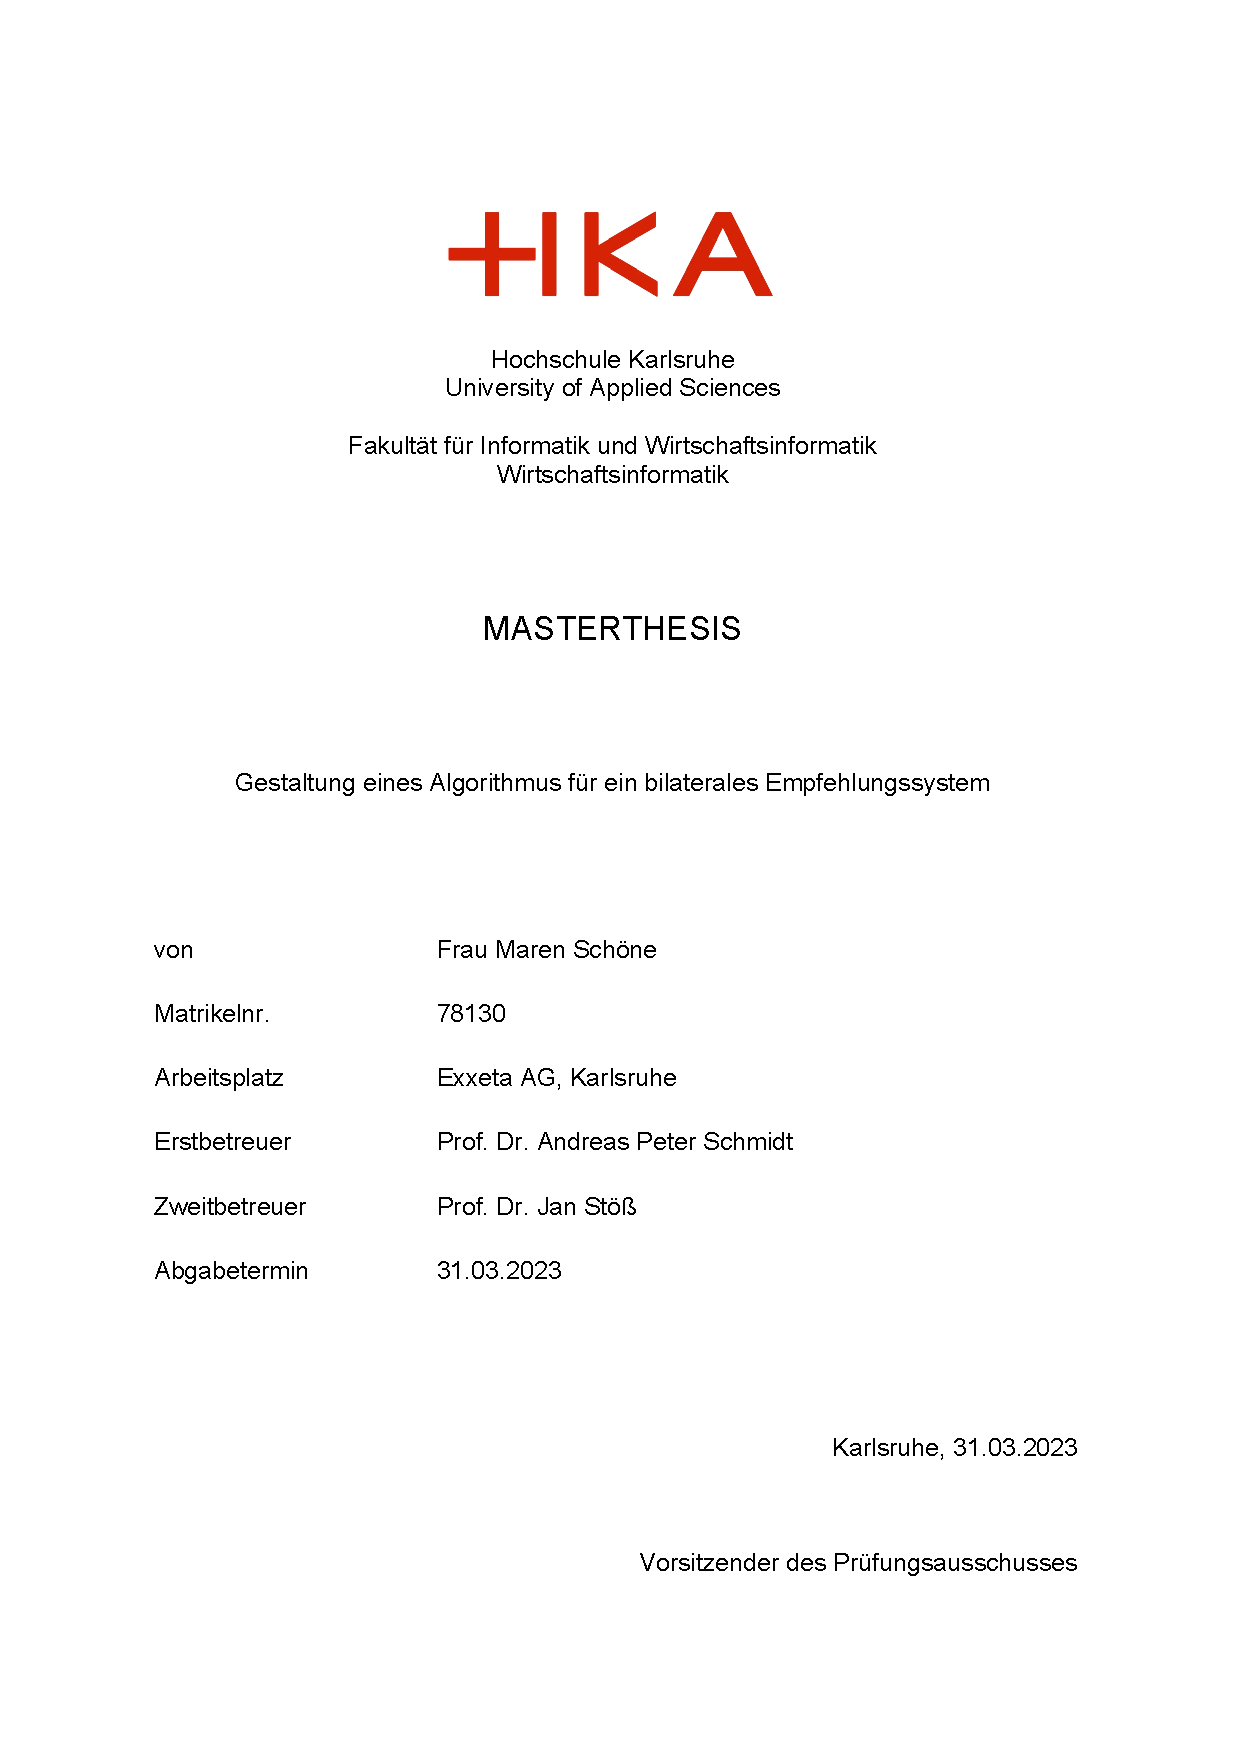
\includepdf[pages=-]{gfx/Deckblatt.pdf}
\end{titlepage}

%%*******************************************************
% Titlepage
%*******************************************************
%%%
%%% title page (german)
%%%
\thispagestyle{empty}
\pdfbookmark[0]{Titelblatt}{title}
\begin{titlepage}

  % If printed on two sides, center the title page
  \condTWOSIDE{\changetext{}{19mm}{}{19mm}{}}

  \vspace{1cm}
  \begin{center}
  	
\includegraphics[width=2.5cm]{gfx/HKA_Logo} \\ 
  \end{center}
  
  \begin{center}
    \huge \textbf{\myUni}\\
    %\huge \textbf{Technik und Wirtschaft}\\
    \vspace{0.4cm}
    \LARGE \myFaculty
  \end{center}

  \vfill
  \vfill

  \begin{center}
    \LARGE \textbf{\myTitle}
  \end{center} 

  \vfill
  \vfill

  \begin{center}
    \Large Abschlussarbeit zur Erlangung des akademischen Grades \textbf{\myDegree}
  \end{center}

  \vfill

  \begin{center}
    \Large vorgelegt von\\
    \vspace{0.3cm}
    \Large \textbf{\myName}\\
    \vspace{0.3cm}
    \normalsize Matrikelnummer: \myId
  \end{center}

  \vfill
  \vfill

  \begin{center}
    \begin{tabular}{lll}
      Referent    & : & \myProf \\
      Korreferent & : & \myOtherProf
    \end{tabular}
  \end{center} 

  % If printed on two sides, center the title page
  \condTWOSIDE{\changetext{}{-19mm}{}{-19mm}{}}

\end{titlepage}

%\thispagestyle{empty}

\hfill

\vfill

\noindent\myName: \textit{\myTitle}, \ifdef{\mySubtitle}{\mySubtitle,}{} %\myDegree,
\textcopyright\ \myTime

%\bigskip
%
%\noindent\spacedlowsmallcaps{Supervisors}: \\
%\myProf \\
%\myOtherProf \\
%\mySupervisor
%
%\medskip
%
%\noindent\spacedlowsmallcaps{Location}: \\
%\myLocation
%
%\medskip
%
%\noindent\spacedlowsmallcaps{Time Frame}: \\
%\myTime

%\cleardoublepage\include{frontbackmatter/Dedication}
%\cleardoublepage\include{frontbackmatter/Foreword}
\cleardoublepage%*******************************************************
% Declaration
%*******************************************************
\refstepcounter{dummy}
\pdfbookmark[0]{Declaration}{declaration}
\chapter*{\condENGLISH{Declaration}{Erklärung}}
\thispagestyle{empty}
Ich versichere hiermit, dass ich die vorliegende Arbeit selbständig verfasst und keine anderen als die im Literaturverzeichnis angegebenen Quellen benutzt habe.
\medskip

\noindent
Alle Stellen, die wörtlich oder sinngemäß aus veröffentlichten oder noch nicht veröffentlichten Quellen entnommen sind, sind als solche kenntlich gemacht.
\medskip

\noindent
Die Zeichnungen oder Abbildungen in dieser Arbeit sind von mir selbst erstellt worden oder mit einem entsprechenden Quellennachweis versehen.
\medskip

\noindent
Diese Arbeit ist in gleicher oder ähnlicher Form noch bei keiner anderen Prüfungsbehörde eingereicht worden. 
\bigskip

\noindent\textit{\myLocation, \myTime}

\smallskip

\begin{flushright}
    \begin{tabular}{m{5cm}}
        \\ \hline
        \centering\myName \\
    \end{tabular}
\end{flushright}

%\cleardoublepage%*******************************************************
% Genderhinweis
%*******************************************************
\refstepcounter{dummy}
\pdfbookmark[0]{Declaration}{declaration}
\chapter*{Gleichstellungsklausel}
\thispagestyle{empty}
Für eine bessere Lesbarkeit wird in dieser Arbeit bei Personenbezeichnungen und personenbezogenen Hauptwörtern die männliche Form verwendet. Entsprechende Begriffe gelten gleichermaßen für alle Geschlechter und beinhalten keine Wertung.

%\cleardoublepage%*******************************************************
% Abstract in English
%*******************************************************
\pdfbookmark[1]{Abstract}{Abstract}


\begin{otherlanguage}{american}
	\chapter*{Abstract}
	Short summary of the contents in English. Approximately one page\dots
	\medskip
	
	\noindent
	BTW: A great guide by Kent Beck how to write good abstracts can be found here:
	\begin{center}
		\url{https://plg.uwaterloo.ca/~migod/research/beckOOPSLA.html}
	\end{center}
\end{otherlanguage}
%\cleardoublepage%*******************************************************
% Abstract in German
%*******************************************************
\begin{otherlanguage}{ngerman}
\pdfbookmark[1]{Zusammenfassung}{Zusammenfassung}
\chapter*{Zusammenfassung}
Der Einsatz von Empfehlungssystemen zur Entscheidungsunterstützung hat in den vergangenen Jahren zunehmend an Bedeutung gewonnen.
Während Empfehlungssysteme ursprünglich für die Empfehlung von Gegenständen oder Dokumenten eingesetzt wurden, hat die Empfehlung von Personen durch den Zuwachs an sozialen Netzwerken vermehrt Aufmerksamkeit erlangt.
In Systemen, in denen Personen die Inhalte von Empfehlungen bilden, kann der Erfolg einer Empfehlung von der Erfüllung der Präferenzen beider beteiligter Parteien, das heißt von sowohl Empfehlungsempfänger als auch empfohlener Person, beeinflusst werden.
Solche Systeme werden als wechselseitige oder auch bilaterale Empfehlungssysteme bezeichnet.

In projektgetriebenen Unternehmen können wechselseitige Empfehlungssysteme Entscheidungsträger darin unterstützen, passende Mitarbeiter offenen Projektpositionen zuzuordnen.
% In der Forschung konnte bereits nachgewiesen werden, dass eine beidseitige Berücksichtigung der Bedürfnisse bei der Empfehlungserstellung im Vergleich zu einer unilateralen Berücksichtigung zu einer Verbesserung der Zufriedenheit von Mitarbeitern sowie der erwarteten Arbeitsleistung dieser führen kann.
Nach aktuellem Stand der Forschung blieb bislang unklar, wie die Präferenzen von Entscheidungsträgern und Mitarbeitern in einem bilateralen Empfehlungssystem einfliessen müssten, um die Zufriedenheit der Mitarbeiter und deren erwartete Arbeitsleistung seitens der Entscheidungsträger bei der Zuordnung der Mitarbeiter zu Projektpositionen robust zu verbessern.
Dieser Fragestellung soll im Rahmen der vorliegenden Arbeit nachgegangen werden.

Hierfür wurde ein multi-kriterieller Ansatz für die Berücksichtigung der Präferenzen von Entscheidungsträgern und Mitarbeitern bei der Zuordnung zu Projekten konzipiert.
Innerhalb des Systems wurde ein bilateraler Algorithmus implementiert, der Empfehlungen anhand der gewichteten Summe der Präferenzerfüllung eines Mitarbeiters und der Präferenzerfüllung eines Entscheidungsträgers ermittelt.
Dessen Tauglichkeit wurde im Rahmen eines Experiments mit einem unilateralen Algorithmus verglichen, welcher lediglich die Bedürfnisse der Entscheidunsträger betrachtet.

Insgesamt zeigten die Ergebnisse des Experiments, dass eine Berücksichtigung der beidseitigen Präferenzen bei der Zuordnung von Mitarbeitern zu Projektpositionen grundsätzlich vorteilhaft ist.
Jedoch konnten einzelne Ausreißer in den Ergebnissen festgestellt werden, bei denen unter diesen Bedingungen eine geringere Zufriedenheit bzw. Arbeitsleistung verzeichnet wurde.
Eine Robustheit des entwickelten Ansatzes kann daher nicht uneingeschränkt bestätigt werden.

Als Ursache für diese Beobachtung wird vermutet, dass sowohl die Zufriedenheit von Mitarbeitern als auch deren erwartete Arbeitsleistung seitens der Entscheidungsträger durch weitere Einflussfaktoren bestimmt werden.
Um den eindeutigen Einfluss der bilateralen Präferenzerfüllung auf Zufriedenheit und Arbeitsleistung zu ermitteln, wird empfohlen, diese Faktoren durch das Durchführen von Experteninterviews unter den Managern und Mitarbeitern zu identifizieren.
Die identifizierten Faktoren sollten in weiterführenden Forschungen als zusätzliche Kriterien des multi-kriteriellen Empfehlungssystems berücksichtigt werden.

Bezüglich der Gewichtung der Präferenzen wurde im Rahmen des Experiments deutlich, dass es eine geringfügigere Rolle spielt, wie die Präferenzen von Entscheidungsträgern bzw. Mitarbeitern gewichtet werden.
Um den Effekt der Gewichtung auf Zufriedenheit und Arbeitsleistung genauer zu untersuchen, wird für weiterführende Forschungen empfohlen, die Fälle genauer zu betrachten, in denen die Bedürfnisse der Entscheidungsträger und die Bedürfnisse der Mitarbeiter miteinander konkurrieren.
Darüber hinaus sollte in zukünftigen Studien die optimalen Gewichtung der Präferenzen anhand einer größeren Datenbasis ermittelt werden, um den Algorithmus gegenüber Ausreißer robuster zu gestalten.

\end{otherlanguage}

%\cleardoublepage%*******************************************************
% Publications
%*******************************************************
\pdfbookmark[1]{Publications}{publications}
\chapter*{Publications}\graffito{This is just an early --~and currently ugly~-- test!}
This might come in handy for PhD theses: some ideas and figures have appeared previously in the following publications:

%\noindent Put your publications from the thesis here. The packages \texttt{multibib} or \texttt{bibtopic} etc. can be used to handle multiple different bibliographies in your document.

\begin{refsection}[ownpubs]
    \small
    \nocite{*} % is local to to the enclosing refsection
    \printbibliography[heading=none]
\end{refsection}

\emph{Attention}: This requires a separate run of \texttt{bibtex} for your \texttt{refsection}, \eg, \texttt{ClassicThesis1-blx} for this file. You might also use \texttt{biber} as the backend for \texttt{biblatex}. See also \url{http://tex.stackexchange.com/questions/128196/problem-with-refsection}.

%\cleardoublepage%*******************************************************
% Acknowledgments
%*******************************************************
\pdfbookmark[1]{Acknowledgments}{acknowledgments}

\begin{flushright}{\slshape
    We have seen that computer programming is an art, \\
    because it applies accumulated knowledge to the world, \\
    because it requires skill and ingenuity, and especially \\
    because it produces objects of beauty.} \\ \medskip
    --- \defcitealias{knuth:1974}{Donald E. Knuth}\citetalias{knuth:1974} \citep{knuth:1974}
\end{flushright}



\bigskip

\begingroup
\let\clearpage\relax
\let\cleardoublepage\relax
\let\cleardoublepage\relax
\chapter*{Acknowledgments}
Put your acknowledgments here.

Many thanks to everybody who already sent me a postcard!

Regarding the typography and other help, many thanks go to Marco 
Kuhlmann, Philipp Lehman, Lothar Schlesier, Jim Young, Lorenzo 
Pantieri and Enrico Gregorio\footnote{Members of GuIT (Gruppo 
Italiano Utilizzatori di \TeX\ e \LaTeX )}, J\"org Sommer, 
Joachim K\"ostler, Daniel Gottschlag, Denis Aydin, Paride 
Legovini, Steffen Prochnow, Nicolas Repp, Hinrich Harms, 
Roland Winkler, Jörg Weber, Henri Menke, Claus Lahiri, 
Clemens Niederberger, Stefano Bragaglia, Jörn Hees, 
Scott Lowe, Dave Howcroft, 
and the whole \LaTeX-community for support, ideas and 
some great software.

\bigskip

\noindent\emph{Regarding \mLyX}: The \mLyX\ port was intially done by
\emph{Nicholas Mariette} in March 2009 and continued by
\emph{Ivo Pletikosi\'c} in 2011. Thank you very much for your
work and for the contributions to the original style.


\endgroup




\cleardoublepage%*******************************************************
% Table of Contents
%*******************************************************
\pagestyle{scrheadings}
\refstepcounter{dummy}
\pdfbookmark[1]{\contentsname}{tableofcontents}
\setcounter{tocdepth}{4} % <-- 2 includes up to subsections in the ToC
\setcounter{secnumdepth}{4} % <-- 3 numbers up to subsubsections
\manualmark
\markboth{\spacedlowsmallcaps{\contentsname}}{\spacedlowsmallcaps{\contentsname}}
\tableofcontents

\cleardoublepage
\cleardoublepage%*******************************************************
% List of Figures
%*******************************************************    
\automark[section]{chapter}
\renewcommand{\chaptermark}[1]{\markboth{\spacedlowsmallcaps{#1}}{\spacedlowsmallcaps{#1}}}
\renewcommand{\sectionmark}[1]{\markright{\thesection\enspace\spacedlowsmallcaps{#1}}}
\refstepcounter{dummy}
\pdfbookmark[1]{\listfigurename}{lof}
\listoffigures

\cleardoublepage

\cleardoublepage%*******************************************************
% List of Tables
%*******************************************************
\automark[section]{chapter}
\renewcommand{\chaptermark}[1]{\markboth{\spacedlowsmallcaps{#1}}{\spacedlowsmallcaps{#1}}}
\renewcommand{\sectionmark}[1]{\markright{\thesection\enspace\spacedlowsmallcaps{#1}}}
\refstepcounter{dummy}
\pdfbookmark[1]{\listtablename}{lot}
\listoftables

\cleardoublepage
\cleardoublepage%*******************************************************
% List of Listings
%*******************************************************      
\automark[section]{chapter}
\renewcommand{\chaptermark}[1]{\markboth{\spacedlowsmallcaps{#1}}{\spacedlowsmallcaps{#1}}}
\renewcommand{\sectionmark}[1]{\markright{\thesection\enspace\spacedlowsmallcaps{#1}}}
\refstepcounter{dummy}
\pdfbookmark[1]{\lstlistlistingname}{lol}
\lstlistoflistings

\cleardoublepage
\cleardoublepage%*******************************************************
% Acronyms
%*******************************************************
\automark[section]{chapter}
\renewcommand{\chaptermark}[1]{\markboth{\spacedlowsmallcaps{#1}}{\spacedlowsmallcaps{#1}}}
\renewcommand{\sectionmark}[1]{\markright{\thesection\enspace\spacedlowsmallcaps{#1}}}
\refstepcounter{dummy}
\pdfbookmark[1]{Abk\"{u}rzungsverzeichnis}{abk\"{u}rzungsverzeichnis}
\markboth{\spacedlowsmallcaps{Abk\"{u}rzungsverzeichnis}}{\spacedlowsmallcaps{Abk\"{u}rzungsverzeichnis}}
\chapter*{Abk\"{u}rzungsverzeichnis}

% Insert your acronyms here
\begin{acronym}[AWGN]%[UML]
  \acro{ESCO}[ESCO]{European Skills/Competences, Qualifications and Occupations}
  %\acro{JES}[JES]{Java Enterprise Solutions}
  \acro{JSON}[JSON]{JavaScript Object Notation}
  \acroplural{JSON}[JSONs]{JSONs}
  \acro{KNN}[KNN]{$k$-nächste Nachbarn}
  \acro{NNA}[NNA]{Nächste Nachbar Analyse (Nearest Neighbor Analysis)}
  \acro{ONet}[O*Net]{Occupational Information Network}
  \acro{PEFit}[P-E Fit]{Person-Environment Fit}
  \acroplural{PEFit}[P-E Fits]{Person-Environment Fits}
  \acro{PJFit}[P-J Fit]{Person-Job Fit}
  \acroplural{PJFit}[P-J Fits]{Person-Job Fits}
  \acro{PCA}[PCA]{Principal Component Analysis}
  \acro{REST}[REST]{Representational State Transfer}
\end{acronym}

\cleardoublepage

%*************************************************************************
% Mainmatter
%*************************************************************************
\cleardoublepage
\pagestyle{scrheadings}
\pagenumbering{arabic}
% Alwas use \cleardoublepage before \part{...}.
\cleardoublepage
\part{Thesis}\label{pt:thesis}
\shorthandoff{"}
\chapter{Einführung}
\label{ch:intro}

\section{Motivation}
\label{sec:intro:motivation}
In Unternehmen aller Branchen ist eine Abkehr von großgewachsenen, zentralen und hierarchischen Organisationsstrukturen zu beobachten. Stattdessen setzen Betriebe zunehmend auf kleine, dezentrale und flexible Teams, welche in Projektarbeiten neue Produkte entwickeln und Dienstleistungen erbringen \cite[S. 3]{elanceEconomy:1999}. Besonders stark nimmt dieser Trend seit Mitte der 1990er Jahre zu \cite[S. 8]{whittington:1999}. Ein Hauptgrund für den Wandel ist die fortschreitende Digitalisierung. Diese ermöglicht kurze Kommunikations- und Entscheidungswege und macht damit zentrale und hierarchische Unternehmensstrukturen zunehmend überflüssig \cite[S. 5]{elanceEconomy:1999}.

Aufgrund dieser Entwicklungen wird die Zusammenstellung von Mitarbeitern für neue Projekte voraussichtlich ein immer häufiger stattfindender Prozess in der Wirtschaft sein. Unterstützung können dabei Empfehlungssysteme im Bereich der Personalauswahl bieten. In der Literatur existieren bereits einige Ansätze zur Implementierung solcher Anwendungen. \textcite[S. 1ff.]{malinowski:2006} zu Folge bieten bestehende Empfehlungssysteme jedoch häufig unzureichende Lösungen, da sich diese zumeist einseitig entweder an Personalverantwortliche oder an Stellensuchende richten. Die Wissenschaftler empfehlen stattdessen die Implementierung bilateraler Empfehlungssysteme. Dieses Konzept basiert auf der Theorie des \acp{PEFit} aus der Berufs- und Organisationspsychologie \cite[S. 2]{guan:2021}\cite[S. 3.f]{malinowski:2006}. Es besagt, dass Mitarbeiter und Personalverantwortliche jeweils eine Angebots- und eine Nachfrageperspektive besitzen. Gleichen sich Angebot und Nachfrage beider Parteien aus, führt dies aus Sicht des Unternehmens zu einer hohen Arbeitsleistung und zugleich aus Perspektive des Mitarbeiters zu einer ausgeprägten Zufriedenheit \cite[S. 6]{su:2015}.

Bisher belegte jedoch noch keine Publikation, dass die Theorie des \acp{PEFit} und die damit verbundenen Ergebnisse auf Seiten von Mitarbeitern und Personalverantwortlichen auch durch Empfehlungssysteme erzielt werden können. Somit ist nicht nachgewiesen, dass der höhere Aufwand zur Implementierung bilateraler Anwendungen gegenüber unilateralen Systemen zur Besetzung offener Projektpositionen gerechtfertigt ist. Diese Forschungslücke soll im Rahmen dieser Master-Thesis geschlossen werden.

\newpage
\section{Zielsetzung}
\label{sec:intro:zielsetzung}
Das Ziel der vorliegenden Master-Thesis besteht darin, die folgende Forschungsfrage zu beantworten:

\forschungsfrage

Um diese Frage zu beantworten, wird ein Experiment mit einer anschließenden Fallstudie durchgeführt. Dabei werden Mitarbeiter eines Beratungsunternehmens im IT-Bereich sowohl von einem uni- als auch von einem bilateralen Empfehlungsverfahren für verschiedene Projektpositionen vorgeschlagen. Anschließend wird evaluiert, ob die verantwortlichen Projektmanager von den empfohlenen Angestellten der bilateralen Anwendung eine höhere Arbeitsleistung erwarten, als von den Vorschlägen des unilateralen Systems. Außerdem wird überprüft, ob die Mitarbeiter zufriedener mit ihrer Positionierung in den Vorschlägen der bilateralen Anwendung sind.

\section{Gang der Arbeit}
\label{sec:intro:gangDerArbeit}
Um die Forschungsfrage der vorliegenden Master-Thesis zu beantworten, werden in den Kapiteln \ref{ch:personEnvironmentFit} und \ref{ch:empfehlungssysteme} zunächst die theoretischen Grundlagen bilateraler Empfehlungssysteme erläutert. Hierzu wird in Kapitel \ref{ch:personEnvironmentFit} das psychologische Konzept des \acp{PEFit} erörtert. Das folgende Kapitel \ref{ch:empfehlungssysteme} enthält einen Überblick über Implementierungsansätzen von Empfehlungssystemen. Dabei werden neben modell- und speicherbasierten Methoden auch hybride Verfahren erläutert. Darüber hinaus werden häufig auftretende Probleme bei der Entwicklung von Empfehlungssystemen geschildert und entsprechende Lösungsmöglichkeiten aufgezeigt. Im folgenden Kapitel \ref{ch:verwandteArbeiten} wird der aktuelle Stand der Forschung behandelt. In diesem Kontext werden verwandte Arbeiten diskutiert und hinsichtlich der Forschungsfrage analysiert. Anschließend wird in Kapitel \ref{ch:methodik} die Methodik der Master-Thesis erläutert. In diesem Zusammenhang werden die implementierte Systemarchitektur und die Gestaltung der Fallstudie dargelegt. Die bei Durchführung der Studie gewonnenen Ergebnisse werden in Kapitel \ref{ch:ergebnisse} vorgestellt. Eine Diskussion der Erkenntnisse findet sich im darauffolgenden Kapitel \ref{ch:diskussion}. Dieses endet mit der Beantwortung der Forschungsfrage und daraus abgeleiteten Empfehlungen für zukünftige Arbeiten. Ein abschließendes Fazit folgt in Kapitel \ref{ch:fazit}.
\shorthandon{"}
\definecolor{exxetagray}{gray}{0.75}
\definecolor{itemcolor}{RGB}{179,217,255}
\definecolor{usercolor}{RGB}{255,204,179}

\shorthandoff{"}
\chapter{Empfehlungssysteme}
\label{ch:empfehlungssysteme}

\section{Einführung}
\label{ch:empfehlungssysteme:einfuehrung}
Der Begriff des Empfehlungssystems ist im englischsprachigen Raum auch unter Bezeichnungen wie Recommender System \cite[S. 1]{lu:2015}, Recommender Engine \cite[S. 1]{panigrahi:2016} und Recommendation System \cite[S. 1]{ebesu:2018} verbreitet. Er wurde erstmals im Jahr 1997 von \textcite[S. 1]{resnick:1997} geprägt. Dass der Begriff gerade zu diesem Zeitpunkt entstand, ist auf die zur damaligen Zeit stark wachsende Internetnutzung und die damit verbundenen einfachen Möglichkeiten zur Sammlung und Auswertung großer Mengen an Nutzerdaten zurückzuführen \cite[S. xvii]{recommenderSystems:2016}.

Heutzutage sind insbesondere große IT-Konzerne wie Amazon, Facebook, Google und Netflix bekannt für den Einsatz von Empfehlungssystemen \cite[S. 1]{zarzour:2018}. Diese Unternehmen nutzen Recommender Engines, um ihren Kunden personalisierte Vorschläge zu den Inhalten ihrer Plattformen anzuzeigen \cite[S. 2]{jeckmans:2013}. Häufig entfällt dabei für den Anwender vollständig die Notwendigkeit einer manuellen Suche \cite[S. 1]{comibingCareer:2013}.

Der Einsatz von Empfehlungssystemen wird in der Literatur kritisch diskutiert. Beispielsweise beobachteten \textcite[S. 17f.]{alfano:2020}, dass das Empfehlungssystem der Videostreaming-Plattform YouTube dazu tendiert, neuen Anwendern zur Verlängerung ihrer Nutzungszeit verschwörungstheoretische Inhalte auszuspielen. Eine Untersuchung von Forschern des sozialen Netzwerks Facebook kam zu dem Ergebnis, dass deren Recommender Engine Nutzern verstärkt Inhalte präsentiert, welche konform mit deren Ideologien sind \cite[S. 2]{bakshy:2015}. \textcite[S. 1ff.]{pariser:2012} prägte für diese Art der Personalisierung den Begriff der Filterblase.

Empfehlungssysteme haben aber auch einen bedeutenden Anteil am wirtschaftlichen Erfolg großer Internetplattformen. So führten beispielsweise \textcite[S. 6f.]{sharma:2015} in einer Studie aus den Jahren 2013 und 2014 etwa 30 Prozent der Seitenaufrufe beim Online-Händler Amazon unmittelbar auf den Einsatz von Empfehlungssystemen zurück. \textcite[S. 5]{gomezuribe:2016} stellten bei einer Analyse der Streaming-Plattform Netflix fest, dass ca. 80 Prozent der Nutzungszeit auf Videos entfiel, welche Nutzern ohne vorherige Suche von einer Recommender Engine angezeigt wurden.

Um solche Vorschläge generieren zu können, suchen Empfehlungssysteme relevante Inhalte basierend auf den Präferenzen der Anwender aus \cite[S. 1]{das:2017}. Zu diesem Zweck müssen benötigte Nutzerdaten zunächst erhoben und in einer maschinell auswertbaren Struktur gespeichert werden.

\section{Zugrundeliegende Datenstruktur}
\label{ch:empfehlungssysteme:arbeitsweise}
Empfehlungssysteme können die Präferenzen ihrer Nutzer sowohl über explizite als auch implizite Rückmeldungen erfassen. Explizites Feedback erhalten Plattformen beispielsweise über abgegebene Produktbewertungen oder "Gefällt mir"-Angaben in sozialen Netzwerken. Um implizite Rückmeldungen auszuwerten, werden häufig Verhaltensweisen der Nutzer aufgezeichnet. Hierbei kann es sich beispielsweise um Suchverläufe oder die Wiedergabedauer von Videos handeln \cite[S. 3]{pu:2012}.

Das gesammelte Feedback überführen Analysten in die Struktur von Matrizen \cite[S. 11f.]{recommenderSystems:2016}. Ein Beispiel für eine Matrix mit explizit erfassten Bewertungen der Fähigkeiten von Mitarbeitern ist in Tabelle \ref{tbl:empfehlungssysteme:arbeitsweise:tbl1} dargestellt.

\begin{table}[h]
	\centering
	\begin{tabular}{c|c|c|c|c|c|c}
	 & \textbf{Java} & \textbf{Python} & \textbf{MySQL} & \textbf{MongoDB} & \textbf{HDFS} & \textbf{Spark}\\ 
	\hline
	\textbf{Doe, Jane}     & ? & 4 & 3 & 3 & ? & ?\\
	\textbf{Doe, John}     & 3 & ? & 2 & ? & 1 & ?\\
	\textbf{Muster, Erika} & ? & ? & ? & ? & 5 & 3\\
	\textbf{Muster, Max}   & 2 & 3 & 1 & ? & ? & ?
	\end{tabular}
	\caption{Beispiel für die Matrixdarstellung von Fähigkeiten}
	\label{tbl:empfehlungssysteme:arbeitsweise:tbl1}
\end{table}

In Tabelle \ref{tbl:empfehlungssysteme:arbeitsweise:tbl1} sind in der ersten Spalte die Mitarbeiter eines Unternehmens gespeichert. Diese werden als Nutzer bezeichnet. In den Kopfzeilen der folgenden Spalten sind verschiedene Fähigkeiten eingetragen. Diese werden Elemente genannt. In der Mitte der Tabelle befinden sich die Bewertungen der Fähigkeiten jedes Nutzers \cite[S. 1f.]{strub:2016}. Im Beispiel aus Tabelle \ref{tbl:empfehlungssysteme:arbeitsweise:tbl1} wurden die expliziten Beurteilungen auf einer Skala von eins bis fünf vergeben. Diese bewerteten Matrix-Einträge werden  als beobachtet oder spezifiziert bezeichnet. Unbewertete Elemente sind mit einem Fragezeichen gekennzeichnet und werden unbeobachtet oder fehlend genannt \cite[S. 8]{recommenderSystems:2016}.

Zahlreiche Wissenschaftler in der Literatur sind sich einig, dass für die Empfehlung geeigneter Kandidaten für eine Stelle bzw. Projektposition ein einfacher Abgleich zwischen gesuchten und vorhandenen Fähigkeiten in der Matrix eine unzureichende Lösung darstellt \cite[S. 1]{enhancingERecruitment:2012}\cite[S. 1]{faerber:2003}\cite[S. 2]{prospect:2010} und der Komplexität der Aufgabe nicht gerecht wird \cite[S. 1]{malinowski:2008}. So kritisierten beispielsweise \textcite[S. 1f.]{mitre:2014}, dass bei einem solchen Ansatz Synonyme und verwandte Fähigkeit nicht in die Suche einbezogen werden. Um diesem Problem zu begegnen, existieren in der Literatur unterschiedliche Ansätze, Recommender Engines zu implementieren. Ein verbreitetes Verfahren ist das kollaborative Filtern.

\section{Kollaboratives Filtern}
\label{ch:empfehlungssysteme:cf}
Ein Ziel von Verfahren im Bereich des kollaborativen Filterns ist das Vorhersagen unbewerteter Einträge in Tabelle \ref{tbl:empfehlungssysteme:arbeitsweise:tbl1}. Unbeobachtete Werte eines Zielnutzers werden dabei über Ähnlichkeitsberechnungen aus vergebenen Beurteilungen anderer Anwender geschlussfolgert \cite[S. 1]{su:2009}.

\textcite[S. 3]{breese:1998} unterschieden zwischen speicher- und modellbasierten Algorithmen. Speicherbasierte Verfahren übertragen sämtliche Nutzer und deren Bewertungen bei der Berechnung von Empfehlungen vollständig in den Hauptspeicher des Rechners. Modellbasierte Verfahren nutzen dagegen Algorithmen aus dem Bereich des Data Minings. Diese werden verwendet, um vor dem Einsatz in der Produktivumgebung statistische Vorhersagemodelle zu entwickeln \cite[S. 3]{breese:1998}\cite[S. 11]{schafer:2007}. Im Folgenden werden unterschiedliche Ansätze vorgestellt, speicher- und modellbasierte Verfahren zu implementieren.

\subsection{Speicherbasierte Verfahren}
\label{ch:empfehlungssysteme:cf:speicherbasiert}
Bei der Entwicklung speicherbasierter Verfahren kommen nachbarschaftsbasierte Algorithmen zum Einsatz \cite[S. 29]{recommenderSystems:2016}. Soll beispielsweise die fehlende Java-Bewertung von Jane Doe in Tabelle \ref{tbl:empfehlungssysteme:arbeitsweise:tbl1} vorhergesagt werden, erfolgt dies über paarweise Ähnlichkeitsberechnungen \cite[S. 2f.]{bharti:2019}. Verwenden Algorithmen dabei die Ähnlichkeiten zwischen Mitarbeitern bzw. Tabellenzeilen zur Vorhersage, werden diese als nutzerorientiert bezeichnet. Greifen Verfahren dagegen auf die Gleichartigkeit zwischen Fähigkeiten bzw. Tabellenspalten zurück, werden sie elementorientiert genannt \cite[S. 1f.]{duong:2018}. Laut \textcite[S. 42]{recommenderSystems:2016} liefern elementorientierte Verfahren häufig präzisere, nutzerorientierte Methoden dafür diversere Ergebnisse. Somit erwartet der Autor, dass die Vorschläge der elementorientierten Ansätze für den Nutzer relevanter erscheinen. Jedoch bemängelte er das hohe Risiko bei diesen Verfahren, dass dem Anwender aufgrund der starken Ähnlichkeit der Elemente entweder alle Vorschläge zusagen oder kein einziger.

Bei der Implementierung nachbarschaftsbasierter Verfahren kommen häufig \ac{KNN}-Algorithmen zum Einsatz \cite[S. 1]{nayak:2018}. Um diese zur Vorhersage der Java-Bewertung von Jane Doe anzuwenden, wird bei elementorientierten Verfahren die Ähnlichkeit zwischen Java und jeder anderen Fähigkeit bestimmt, welche Jane Doe beherrscht. Anschließend wird die durchschnittliche Bewertung der k-ähnlichsten Fähigkeiten berechnet und als Java-Beurteilung für Jane Doe eingesetzt \cite[S. 2]{hao:2013} Welcher Wert für k verwendet werden sollte, kann pauschal nicht beantwortet werden. Beispielsweise ist es möglich, Verfahren aus dem Bereich des maschinellen Lernens zu nutzen, um abhängig von den vorhandenen Daten einen geeigneten Wert für k zu ermitteln \cite[S. 2f.]{jiang:2007}.

Bei nutzerorientierten Algorithmen wird die Gleichartigkeit zwischen Jane Doe und allen anderen Mitarbeitern berechnet. Daraufhin wird die durchschnittliche Java-Beurteilung der k-ähnlichsten Mitarbeiter bestimmt und als Java-Bewertung für Jane Doe vorhergesagt \cite[S. 2f.]{hao:2013}.

Zur Ähnlichkeitsberechnung können unterschiedliche Algorithmen wie die Jaccard-Ähnlichkeit \cite[S. 2]{bharti:2019}, die euklidische Distanz \cite[S. 3]{cheng:2013} oder die Kosinus-Ähnlichkeit \cite[S. 2]{duong:2018} verwendet werden. Beispielhaft ist in der folgenden Gleichung \ref{fig:empfehlungssysteme:cf:speicherbasiert:formel1} die Formel zur Berechnung der Kosinus-Ähnlichkeit zwischen zwei Vektoren A und B dargestellt \cite[S. 111]{bharti:2019}.
\begin{equation}
cos(A,B) = \frac{(\vec{A} * \vec{B})}{|\vec{A}| * |\vec{B}|} = \frac{\sum_{i=1}^n A_i * B_i}{\sqrt{\sum_{i=1}^n (A_i)^2} * \sqrt{\sum_{i=1}^n (B_i)^2}}
\label{fig:empfehlungssysteme:cf:speicherbasiert:formel1}
\end{equation}
Anstelle der Vektoren A und B können in Gleichung \ref{fig:empfehlungssysteme:cf:speicherbasiert:formel1} paarweise die Spalten/Fähigkeiten bzw. Zeilen/Mitarbeiter aus Tabelle \ref{tbl:empfehlungssysteme:arbeitsweise:tbl1} eingesetzt werden.

Gleichung \ref{fig:empfehlungssysteme:cf:speicherbasiert:formel2} zeigt die nutzerbasierte Ähnlichkeitsberechnung zwischen Jane Doe und Max Muster anhand der Daten aus Tabelle \ref{tbl:empfehlungssysteme:arbeitsweise:tbl1}. Dort ist zu erkennen, dass ausschließlich Tabellenspalten in die Berechnung einbezogen werden, welche beide Mitarbeiter bewertet haben \cite[S. 2f.]{hao:2013}.
\begin{equation}
	cos(Jane Doe,Max Muster) = \frac{(4*3 + 3*1)}{\sqrt{4^2 + 3^2} * \sqrt{3^2 + 1^2}} \approx \frac{15}{15,811} \approx 0,95
	\label{fig:empfehlungssysteme:cf:speicherbasiert:formel2}
\end{equation}
Wie in der folgenden Gleichung \ref{fig:empfehlungssysteme:cf:speicherbasiert:formel3} dargestellt, kann analog auch die elementbasierte Ähnlichkeit für Java und MySQL aus Tabelle \ref{tbl:empfehlungssysteme:arbeitsweise:tbl1} mittels Kosinus-Distanz berechnet werden.
\begin{equation}
	cos(Java, MySQL) = \frac{(3*2 + 2*1)}{\sqrt{3^2 + 2^2} * \sqrt{2^2 + 1^2}} \approx \frac{8}{8,063} \approx 0,992
	\label{fig:empfehlungssysteme:cf:speicherbasiert:formel3}
\end{equation}
In den Gleichungen \ref{fig:empfehlungssysteme:cf:speicherbasiert:formel2} und \ref{fig:empfehlungssysteme:cf:speicherbasiert:formel3} ist zu erkennen, dass im vorliegenden Beispiel eine Ähnlichkeit zwischen Jane Doe und Max Muster von 95 Prozent und eine Gleichartigkeit von 99,2 Prozent zwischen Java und MySQL besteht.%Um über nutzerbasiertes kollaboratives Filtern die Java-Bewertung von Jane Doe vorherzusagen, müsste zusätzlich die Ähnlichkeit zwischen Jane Doe und allen anderen Nutzern in der Datenbank bestimmt werden. Anschließend könnte das Empfehlungssystem die k ähnlichsten Nutzer zu Jane Doe auswählen und deren durchschnittliche Java-Bewertung als Fähigkeitseinschätzung bei Jane Doe einsetzen. 

\textcite[S. 35ff.]{recommenderSystems:2016} kritisierte an solchen Ähnlichkeitsberechnungen, dass möglicher Bias die Ergebnisse verzerren kann. So könnten einzelne Mitarbeiter ihre Fähigkeiten grundsätzlich schlechter oder besser einschätzen als andere Angestellte. Aus diesem Grund empfahl der Autor, vor den Ähnlichkeitsberechnungen zunächst eine Mittelwert-Zentrierung auszuführen. Hierbei wird in Tabelle \ref{tbl:empfehlungssysteme:arbeitsweise:tbl1} die durchschnittliche Bewertung jedes Nutzers bestimmt und von dessen vorhandenen Beurteilungen abgezogen. Dabei entstehende negative Bewertungen müssen anschließend aus der Tabelle entfernt werden. Dieses Vorgehen ist in der Literatur auch unter der Bezeichnung Pearson Korrelation bekannt \cite[S. 3]{bharti:2019}.

Es gilt zu beachten, dass die bisher vorgestellten Algorithmen im Bereich des speicherbasierten kollaborativen Filterns anfällig für das Sparsity Problem sind \cite[S. 3f.]{grvcar:2006}. Dieses bezeichnet das Phänomen, dass in der Praxis meist für einen Bruchteil aller Spalten sehr viele Bewertungen und für einen Großteil der Elemente nur sehr wenige Beurteilungen vorliegen \cite[S. 8]{recommenderSystems:2016}. So stellten beispielsweise \textcite[S. 3]{mitre:2014} bei der Implementierung ihres Projekt-Empfehlungssystems fest, dass über die Hälfte der ca. 17.000 vergebenen Fähigkeiten von nur je einem Mitarbeiter angegeben wurden.
Für diese Häufigkeitsverteilung prägte \textcite[S. 12]{anderson:2007} den Begriff des langen (Ratten-)Schwanzes (Long Tail). Erkennbar wird dieser, wenn Bewertungen, wie in Abbildung \ref{fig:empfehlungssysteme:cf:speicherbasiert:abb1} dargestellt, in Form eines Diagramms aggregiert werden.

\begin{figure}[h]
	\centering
	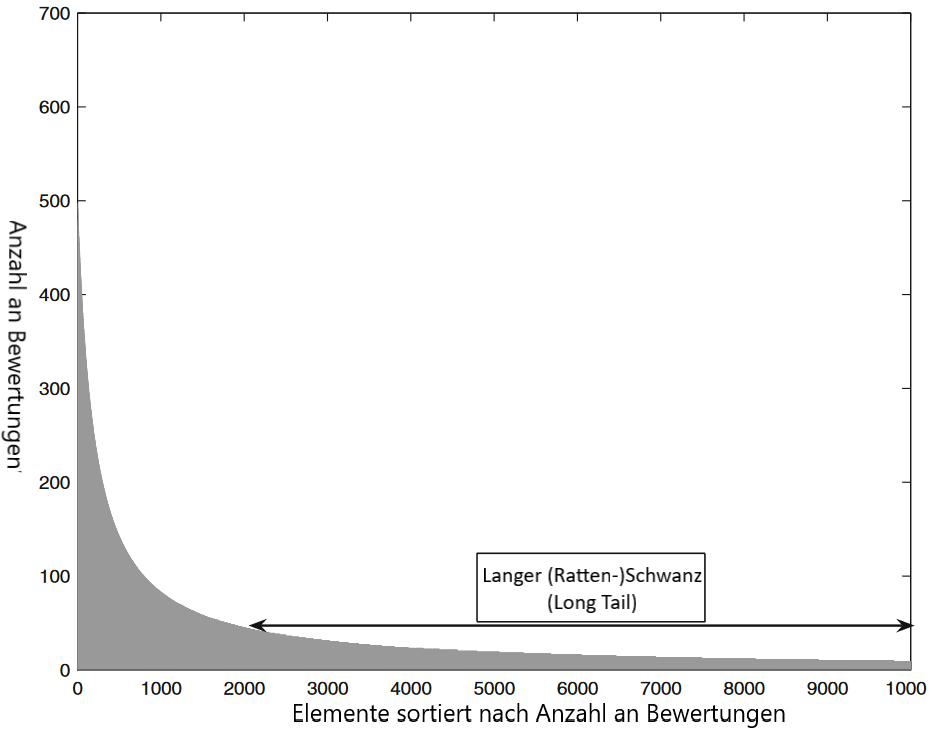
\includegraphics[width=1\textwidth]{gfx/long-tail.png}
	\caption[Darstellung des langen (Ratten-)Schwanzes]{Darstellung des langen (Ratten-)Schwanzes\\
		(Eigene Darstellung in Anlehnung an \cite[S. 33]{recommenderSystems:2016})}
	\label{fig:empfehlungssysteme:cf:speicherbasiert:abb1}
\end{figure}

Die in Abbildung \ref{fig:empfehlungssysteme:cf:speicherbasiert:abb1} dargestellte Häufigkeitsverteilung von abgegebenen Bewertungen spiegelt \textcite[S. 1ff.]{anderson:2007} zu Folge einen allgemeinen Trend wider, welchen er im Zusammenhang mit der Digitalisierung beobachtet. Der Autor stellte fest, dass sich Menschen aufgrund der heute verfügbaren breiten Angebote wesentlich diverser orientieren, als es vor einigen Jahrzehnten der Fall war \cite[S. 1ff.]{anderson:2007}.

Das Sparsity Problem kann auch in Tabelle \ref{tbl:empfehlungssysteme:arbeitsweise:tbl1} beobachtet werden. Dort haben MongoDB und Spark jeweils nur eine Bewertung. Für diese Fähigkeiten ist es über Ähnlichkeitsberechnungen im Bereich des speicherbasierten kollaborativen Filterns somit nicht möglich, für alle Angestellten robuste Vorhersagen zu ermitteln.

Um diesem Problem zu begegnen, kann die bisher verwendete Matrixdarstellung in die Form eines bipartiten Graphen überführt werden \cite[S. 2f.]{huang:2004}. Diese Datenstruktur zeichnet sich durch die Verwendung zwei unterschiedlicher Arten von Knoten zur separaten Speicherung von Nutzern und Elementen aus. Bewertungen werden bei dieser Darstellungsform über gewichtete Kanten im Graphen dargestellt \cite[S. 1f.]{cao:2021}.

Abbildung \ref{fig:empfehlungssysteme:cf:speicherbasiert:abb2} zeigt die Fähigkeitsmatrix aus Tabelle \ref{tbl:empfehlungssysteme:arbeitsweise:tbl1} in der Datenstruktur eines bipartiten Graphen. In der Darstellung sind die Knoten der Mitarbeiter rot und die Knoten der Fähigkeiten blau markiert.

\begin{figure}[h]
	\centering	
	\begin{tikzpicture}[node distance={32mm}, thick, main/.style = {draw, circle}] 
		\node[main, fill=itemcolor] (MongoDB) {$MongoDB$}; 
		\node[main, fill=itemcolor] (Python) [below right of=MongoDB] {$Python$}; 
		\node[main, fill=itemcolor] (MySQL) [above right of=Python] {$MySQL$}; 
		\node[main, fill=itemcolor] (Java) [below right of=MySQL] {$Java$}; 
		\node[main, fill=itemcolor] (HDFS) [above right of=Java] {$HDFS$}; 
		\node[main, fill=itemcolor] (Spark) [below right of=HDFS] {$Spark$};
		
		\node[main, fill=usercolor] (Jane) [above right of=MongoDB] {$Jane D.$}; 
		\node[main, fill=usercolor] (John) [above left of=HDFS] {$John D.$}; 
		\node[main, fill=usercolor] (Max) [below of=MySQL] {$Max M.$};
		\node[main, fill=usercolor] (Erika) [above right of=HDFS] {$Erika M.$}; 
		
		\draw (Jane) -- node[midway, right] {4} (Python);
		\draw (Jane) -- node[midway, above] {3} (MySQL);
		\draw (Jane) -- node[midway, above] {3} (MongoDB);

		\draw (John) -- node[midway, right] {1} (HDFS);		
		\draw (John) -- node[midway, right] {3} (Java);
		\draw (John) -- node[midway, above] {2} (MySQL);
		
		%\path (Erika) edge[bend right=10] node[midway, right] {5} (HDFS); 
		\draw (Erika) -- node[midway, above] {5} (HDFS);
		\draw (Erika) -- node[midway, right] {3} (Spark);
		
		\draw (Max) -- node[midway, above] {2} (Java);
		\draw (Max) -- node[midway, above] {3} (Python);
		\draw (Max) -- node[midway, right] {1} (MySQL);
	\end{tikzpicture}

	\caption{Darstellung der Fähigkeitsmatrix aus Tabelle \ref{tbl:empfehlungssysteme:arbeitsweise:tbl1} in der Datenstruktur eines Graphen}
	\label{fig:empfehlungssysteme:cf:speicherbasiert:abb2}
\end{figure}

\textcite[S. 7ff.]{huang:2004} bemerkten mit Blick auf bipartite Graphen, dass bei klassischen nachbarschaftsbasierten Algorithmen nur Empfehlungen für Knoten bestimmt werden können, welche von einem Zielknoten über drei Kanten zu erreichen sind. Somit könnten in der vorliegenden Abbildung \ref{fig:empfehlungssysteme:cf:speicherbasiert:abb2} über solche Verfahren beispielsweise keine Bewertungsvorhersagen für Jane Doe und Spark oder Erika Muster und MongoDB bestimmt werden.

Um auch in solchen Fällen Empfehlungen zu generieren, ist der Einsatz graphenbasierter Algorithmen empfehlenswert. Diese können über transitive Verbindungen auch weiter entfernte Knoten in die Berechnung mit einbeziehen \cite[S. 60f.]{recommenderSystems:2016}.

Ein in der Literatur häufig angewendeter Graphenalgorithmus ist die Katz-Zentralität \cite[S. 6]{guns:2014}\cite[S. 1f.]{huang:2004}\cite[S. 1ff.]{zhan:2017}. Diese basiert auf einem im Jahr 1953 vorgestellten mathematischen Verfahren von \textcite[S. 1ff.]{katz:1953}, welches dieser zur Bestimmung von Anführern in sozialen Gruppen entwickelte. Heute nutzen graphenbasierte Empfehlungssysteme diesen Algorithmus beispielsweise zur Verbindungsvorhersage. Diese Problemstellung ist unter anderem im Bereich der sozialen Netzwerke verbreitet und verfolgt das Ziel, aus vorhandenen Kanten im Graphen bisher unbekannte Verbindungen vorherzusagen \cite[S. 1ff.]{libenNowell:2007}.

Der Algorithmus von Katz basiert auf folgender Gleichung \ref{frml:empfehlungssysteme:cf:speicherbasiert:formel4} \cite[S. 4]{libenNowell:2007}.
\begin{equation}
	(I - \beta * M)^{-1} - I
	\label{frml:empfehlungssysteme:cf:speicherbasiert:formel4}
\end{equation}
In Gleichung \ref{frml:empfehlungssysteme:cf:speicherbasiert:formel4} steht $\beta$ für eine Zahl im Bereich von \nullWert bis eins \cite[S. 6]{guns:2014}, welche jedoch stets kleiner als $1/\lambda$ sein muss. $\lambda$ entspricht dabei dem größten Eigenwert der Matrix M \cite[S. 6]{zhan:2017}. Je größer der Wert von $\beta$ angesetzt wird, desto stärker werden weit entfernte Beziehungen in der Berechnung gewichtet \cite[S. 6]{guns:2014}.
% TODO: Das nochmal prüfen

Die Variable $I$ steht in Gleichung \ref{frml:empfehlungssysteme:cf:speicherbasiert:formel4} für die Einheitsmatrix. $M$ symbolisiert die Adjazenzmatrix des betrachteten Graphen \cite[S. 4]{libenNowell:2007}. Diese gibt an, wie viele Kanten von einem Startknoten zu jedem anderen Knoten führen \cite[S. 6]{guns:2014}. Der mit Zahlen versehene Bereich von Tabelle \ref{tbl:empfehlungssysteme:arbeitsweise:tbl2} entspricht der Adjazenzmatrix für den Graphen aus Abbildung \ref{fig:empfehlungssysteme:cf:speicherbasiert:abb2}.

\begin{table}[h]
	\centering
	\begin{tabular}{c|c|c|c|c|c|c|c|c|c|c}
		& \begin{sideways}\textbf{Jane D.}\end{sideways} & \begin{sideways}\textbf{John D.}\end{sideways} & \begin{sideways}\textbf{Erika M.}\end{sideways} & \begin{sideways}\textbf{Max M.}\end{sideways} & \begin{sideways}\textbf{Java}\end{sideways} & \begin{sideways}\textbf{Python}\end{sideways} & \begin{sideways}\textbf{MySQL}\end{sideways} & \begin{sideways}\textbf{MongoDB}\end{sideways} & \begin{sideways}\textbf{HDFS}\end{sideways} & \begin{sideways}\textbf{Spark}\end{sideways} \\
		\hline
		\textbf{Jane D.}  & 0 & 0 & 0 & 0 & 0 & 4 & 3 & 3 & 0 & 0\\
		\textbf{John D.}  & 0 & 0 & 0 & 0 & 3 & 0 & 2 & 0 & 1 & 0\\
		\textbf{Erika M.} & 0 & 0 & 0 & 0 & 0 & 0 & 0 & 0 & 5 & 3\\
		\textbf{Max M.}   & 0 & 0 & 0 & 0 & 2 & 3 & 1 & 0 & 0 & 0\\
		\textbf{Java}     & 0 & 3 & 0 & 2 & 0 & 0 & 0 & 0 & 0 & 0\\
		\textbf{Python}   & 4 & 0 & 0 & 3 & 0 & 0 & 0 & 0 & 0 & 0\\
		\textbf{MySQL}    & 3 & 2 & 0 & 1 & 0 & 0 & 0 & 0 & 0 & 0\\
		\textbf{MongoDB}  & 3 & 0 & 0 & 0 & 0 & 0 & 0 & 0 & 0 & 0\\
		\textbf{HDFS}     & 0 & 1 & 5 & 0 & 0 & 0 & 0 & 0 & 0 & 0\\
		\textbf{Spark}    & 0 & 0 & 3 & 0 & 0 & 0 & 0 & 0 & 0 & 0
	\end{tabular}
	\caption{Anzahl an Verbindungen im Graphen aus Abbildung \ref{fig:empfehlungssysteme:cf:speicherbasiert:abb2}}
	\label{tbl:empfehlungssysteme:arbeitsweise:tbl2}
\end{table}

Für Tabelle \ref{tbl:empfehlungssysteme:arbeitsweise:tbl2} ergeben sich mit $\beta = 0.125$ durch Anwendung des Katz-Algorithmus die in Tabelle \ref{tbl:empfehlungssysteme:arbeitsweise:tbl3} dargestellten Werte. Die vollständige Berechnung kann in Appendix \ref{ch:nebenrechnungen:katzZentralitaet} nachvollzogen werden.

\begin{table}[h]
	\centering
	\begin{tabular}{c|c|c|c|c|c|c|c|c|c|c}
		& \begin{sideways}\textbf{Jane D.}\end{sideways} & \begin{sideways}\textbf{John D.}\end{sideways} & \begin{sideways}\textbf{Erika M.}\end{sideways} & \begin{sideways}\textbf{Max M.}\end{sideways} & \begin{sideways}\textbf{Java}\end{sideways} & \begin{sideways}\textbf{Python}\end{sideways} & \begin{sideways}\textbf{MySQL}\end{sideways} & \begin{sideways}\textbf{MongoDB}\end{sideways} & \begin{sideways}\textbf{HDFS}\end{sideways} & \begin{sideways}\textbf{Spark}\end{sideways} \\ 
		\hline
		\textbf{Jane D.}  & 1.66 & 0.47 & 0.08 & 0.87 & 0.39 & 1.66 & 1.22 & 1.00 & 0.11 & 0.03\\
		\textbf{John D.}  & 0.47 & 0.42 & 0.24 & 0.37 & 0.62 & 0.37 & 0.58 & 0.18 & 0.33 & 0.09\\
		\textbf{Erika M.} & 0.08 & 0.24 & 1.17 & 0.06 & 0.10 & 0.06 & 0.10 & 0.03 & 1.39 & 0.81\\
		\textbf{Max M.}   & 0.87 & 0.37 & 0.06 & 0.60 & 0.54 & 1.04 & 0.62 & 0.33 & 0.08 & 0.02\\
		\textbf{Java}     & 0.39 & 0.62 & 0.10 & 0.54 & 0.37 & 0.40 & 0.37 & 0.15 & 0.14 & 0.04\\
		\textbf{Python}   & 1.66 & 0.37 & 0.06 & 1.04 & 0.40 & 1.22 & 0.84 & 0.62 & 0.09 & 0.02\\
		\textbf{MySQL}    & 1.22 & 0.58 & 0.10 & 0.62 & 0.37 & 0.84 & 0.68 & 0.46 & 0.13 & 0.04\\
		\textbf{MongoDB}  & 1.00 & 0.18 & 0.03 & 0.33 & 0.15 & 0.62 & 0.46 & 0.37 & 0.04 & 0.01\\
		\textbf{HDFS}     & 0.11 & 0.33 & 1.39 & 0.08 & 0.14 & 0.09 & 0.13 & 0.04 & 0.91 & 0.52\\
		\textbf{Spark}    & 0.03 & 0.09 & 0.81 & 0.02 & 0.04 & 0.02 & 0.04 & 0.01 & 0.52 & 0.31
	\end{tabular}
	\caption{Berechnete Katz-Zentralität mit $\beta = 0.125$ für Tabelle \ref{tbl:empfehlungssysteme:arbeitsweise:tbl2}}
	\label{tbl:empfehlungssysteme:arbeitsweise:tbl3}
\end{table}

In Tabelle \ref{tbl:empfehlungssysteme:arbeitsweise:tbl3} ist zu erkennen, dass durch Bestimmung der Katz-Zentralität für sämtliche Knoten die Stärke der Verbindung zu allen anderen Knoten vorhergesagt werden konnte. Das Sparsity Problem wurde somit behoben.

An den Werten in Tabelle \ref{tbl:empfehlungssysteme:arbeitsweise:tbl3} ist zu beobachten, dass der Algorithmus von Katz nicht geeignet ist, fehlende Bewertungen von Mitarbeitern vorherzusagen. Die Anwendung des Algorithmus führt jedoch zu einer feingranularen Anpassung und Glättung der Ausgangsbewertung auf einem veränderten Skalenniveau. So beurteilte beispielsweise Jane Doe die Kompetenzen MongoDB und MySQL in Tabelle \ref{tbl:empfehlungssysteme:arbeitsweise:tbl1} ursprünglich mit gleichen Bewertungen. Nach Berechnung des Katz-Algorithmus ist MySQL in Tabelle \ref{tbl:empfehlungssysteme:arbeitsweise:tbl3} feingranular besser bewertet als MongoDB. Dieses Phänomen ist darauf zurückzuführen, dass MySQL von mehreren Kollegen von Jane Doe ebenfalls bewertet wurde. Somit ist es naheliegend, dass sie diese Kompetenz besser beherrscht als MongoDB.

%In Tabelle \ref{tbl:empfehlungssysteme:arbeitsweise:tbl3} ist außerdem festzustellen, dass die Skalierung der Bewertungen verändert wurde. Projekt-Anforderungen, welche auf der in Tabelle \ref{tbl:empfehlungssysteme:arbeitsweise:tbl2} verwendeten Bewertungsskala spezifiziert wurden, könnte ein Algorithmus somit nicht ohne weiteres mit den Ergebnissen aus Tabelle \ref{tbl:empfehlungssysteme:arbeitsweise:tbl3} abgleichen.
%Eine Lösungsmöglichkeit zeigen Algorithmen von Gruppen-Recommender Engines auf. Solche Systeme verfolgen das Ziel, gemeinsame Vorschläge für mehrere Anwender zu generieren \cite[S. 1]{dara:2020}. Ein in diesem Zusammenhang angewendetes Verfahren ist das Erstellen eines Pseudonutzers, welcher die Präferenzen aller Gruppenmitglieder vereint. Der Pseudonutzer wird bei der Empfehlungsberechnung als gewöhnlicher Anwender betrachtet und beispielsweise in Tabelle \ref{tbl:empfehlungssysteme:arbeitsweise:tbl1} in eine neue Zeile eingefügt. Dieses Vorgehen ermöglicht es, die bisher vorgestellten Verfahren im Bereich des kollaborativen Filterns ohne zusätzliche Komplexität auch zur Bestimmung von Vorschlägen für Gruppen anzuwenden \cite[S. 8f.]{oconnor:2001}.
%Ein vergleichbarer Ansatz könnte auch zur Bestimmung der Katz-Zentralität genutzt werden. Hierfür müsste ein Algorithmus zunächst Tabelle \ref{tbl:empfehlungssysteme:arbeitsweise:tbl2} um eine Zeile erweitern, in welcher das zu besetzende Projekt mitsamt den dafür benötigten Fähigkeiten als Pseudomitarbeiter einfügt wird. Nach der anschließenden Bestimmung der Katz-Zentralität würden auch die Fähigkeiten des Pseudomitarbeiters der neuen Skalierung entsprechen. Somit könnten diese neuen Fähigkeitsbewertungen als Ausgangspunkt für die Bestimmung passender Mitarbeiter für das Projekt verwendet werden. Ein vergleichbares Verfahren wendeten auch \textcite[S. 2]{mitre:2014} bei der Implementierung ihres Empfehlungssystems zur Projektbesetzung an. Die Wissenschaftler nutzen jedoch statt Graphenalgorithmen klassische Verfahren zur Ähnlichkeitsberechnung.

Nah verwandt mit dem Verfahren von Katz ist der PageRank-Algorithmus \cite[S. 1]{was:2018}. Dieser nutzt Kanten zur Darstellung von Verlinkungen im Internet. Auf dieser Grundlage bestimmte Google in seiner Anfangszeit die Priorisierung von Webseiten in deren Suchergebnissen \cite[S. 3ff.]{page:1999}.

Unabhängig von der konkreten Art der Implementierung besteht ein großer Nachteil bei speicherbasierten Verfahren darin, dass bei jeder Empfehlungsberechnung sämtliche Nutzer, Elemente und Bewertungen in den Hauptspeicher geladen werden müssen \cite[S. 8]{yang:2016}. Dies kann zu sehr hohen Laufzeiten führen \cite[S. 2]{zhang:2010}. So bemerken beispielsweise \textcite[S. 3]{landherr:2010}, dass alleine die Invertierung der Matrix bei Berechnung des Katz-Algorithmus mit Gleichung \ref{frml:empfehlungssysteme:cf:speicherbasiert:formel4} eine Komplexität von $O(n^3)$ besitzt. Aus diesen Gründen ist die Verwendung speicherbasierter Ansätze bei großen Datensätzen als ungeeignet zu bewertet. Abhilfe bei steigender Datenmenge können modellbasierte Verfahren bieten \cite[S. 8]{yang:2016}.

\subsection{Modellbasierte Verfahren}
\label{ch:empfehlungssysteme:cf:modellbasiert}
Modellbasierte Verfahren verwenden Ansätze aus dem Bereich des Data Minings zur Generierung von Vorschlägen. Hierbei berechnen Wissenschaftler statistische Modelle, bevor sie ihr Empfehlungssystem den Nutzern zur Verfügung stellen \cite[S. 2]{cui:2020}. Dieses Vorgehen hat den Vorteil, dass in der Produktivumgebung keine Berechnungen mehr auf allen Daten ausgeführt werden müssen. Somit ist die Vorschlagsbestimmung insbesondere bei großen Datenmengen effizienter als bei speicherbasierten Verfahren \cite[S. 8]{yang:2016}.

Wie in Tabelle \ref{tbl:empfehlungssysteme:cf:modellbasiert:tbl1} dargestellt, ist es bei modellbasierten Verfahren üblich, den vorhandenen Datensatz in Trainings- (rot) und Testdaten (blau) zu untergliedern \cite[S. 71f.]{recommenderSystems:2016}. Die Einteilung in der Tabelle erfolgte dabei zufällig.

\begin{table}[h]
	\centering
	\begin{tabular}{c|c|c|c|c|c|c}
		& \textbf{Java} & \textbf{Python} & \textbf{MySQL} & \textbf{MongoDB} & \textbf{HDFS} & \textbf{Spark}\\ 
		\hline
		\textbf{Doe, Jane} & ? & \cellcolor{itemcolor}4 & \cellcolor{itemcolor}3 & \cellcolor{usercolor}3 & ? & ?\\
		\textbf{Doe, John} & \cellcolor{itemcolor}3 & ? & \cellcolor{usercolor}2 & ? & \cellcolor{usercolor}1 & ?\\
		\textbf{Muster, Erika} & ? & ? & ? & ? & \cellcolor{itemcolor}5 & \cellcolor{usercolor}3\\
		\textbf{Muster, Max} & \cellcolor{itemcolor}2 & \cellcolor{usercolor}3 & \cellcolor{itemcolor}1 & ? & ? & ?\\
	\end{tabular}
	\caption{Beispielhafte Unterteilung einer Matrix in Trainings- und Testdaten}
	\label{tbl:empfehlungssysteme:cf:modellbasiert:tbl1}
\end{table}

Die Trainingsdaten werden genutzt, um statistische Modelle zur Vorhersage von Bewertungen zu entwickeln \cite[S. 71f.]{recommenderSystems:2016}. Die Testdaten dienen zur anschließenden Evaluierung und Bewertung hinsichtlich der Genauigkeit des erstellten Modells. Hierbei ist es beispielsweise möglich, bekannte Einträge von Testdaten in der Matrix temporär zu entfernen, diese anschließend durch das trainierte Modell vorherzusagen und daraufhin tatsächliche und vorhergesagte Werte zu vergleichen \cite[S. 3ff.]{kang:2016}.
% die Implementierung neuronaler Netze \cite[S. 5ff.]{personJobFit:2018}, die Anwendung des naiven Bayes-Klassifikators \cite[S. 2]{valdividezodiaz:2019}, die Durchführung von Matrix-Faktorisierungsverfahren \cite[S. 2ff.]{ortega:2016} oder die Berechnung von Entscheidungsbäumen \cite[S. 1ff.]{yu:2012} verbreitet.

Wie an den Spalten in Tabelle \ref{tbl:empfehlungssysteme:cf:modellbasiert:tbl1} zu erkennen ist, existieren in der Praxis häufig sehr viele Merkmale bzw. Dimensionen, welche zur Entwicklung von Modellen relevant sein können. Zusätzlich sind Matrizen, wie in Kapitel \ref{ch:empfehlungssysteme:cf:speicherbasiert} beschrieben, in der Praxis aufgrund des Sparsity Problems meist sehr schwach besetzt. \textcite[S. 1]{boratto:2014} stellten fest, dass in solchen Situationen, in welchen viele Dimensionen und gleichzeitig wenige Daten vorliegen, keine statistisch aussagekräftigen Modelle erstellt werden können. \textcite[S. 94, Z. 7]{bellman:1961} prägte für diesen Sachverhalt den Ausdruck "Fluch der Dimensionalität"\footnote{"Curse of Dimensionality" - \textcite[S. 94, Z. 7]{bellman:1961}}. Um in solchen Situationen dennoch Empfehlungen generieren zu können, stellten verschiedene Autoren in der Literatur Verfahren zur Dimensionsreduzierung vor. Verbreitet ist dabei beispielsweise die Hauptkomponentenanalyse, welche im englischsprachigen Raum als \ac{PCA} bezeichnet wird \cite[S. 1ff.]{vaswani:2018}.

\textcite[S. 1f.]{pennock:2000} kritisierten an modellbasierten Verfahren, dass diese stets den Zustand der Daten zum Zeitpunkt des Trainings des Modells abbilden. Werden beispielsweise Fähigkeiten in der Datenbank hinzugefügt bzw. entfernt oder Bewertungen signifikant verändert, muss gegebenenfalls das statistische Modell neu trainiert werden, um diese Anpassungen zu erfassen. Speicherbasierte Verfahren können den Autoren zu Folge solche Änderungen dagegen unmittelbar berücksichtigen \cite[S. 1f.]{pennock:2000}.

Ein Problem, welches weder speicher- noch modellbasierte Verfahren im Bereich des kollaborativen Filterns zuverlässig lösen können, ist der sogenannte Kaltstart. Dieser tritt auf, wenn neue Nutzer oder Fähigkeiten in die Datenbank hinzugefügt werden, welchen noch keine Bewertung zugeordnet ist \cite[S. 5]{huang:2004}. In solchen Fällen ist die gesamte Zeile bzw. Spalte in Tabelle \ref{tbl:empfehlungssysteme:arbeitsweise:tbl1} mit fehlenden Einträgen gekennzeichnet. Im entsprechenden Graphen in Abbildung \ref{fig:empfehlungssysteme:cf:speicherbasiert:abb2} existiert somit keine Kante von der betrachteten Entität zu anderen Knoten. Daher ist es weder über speicherbasierte Ähnlichkeitsberechnungen, noch graphenbasierte Algorithmen oder statistische Modelle möglich, zuverlässige Vorhersagen mittels kollaborativem Filtern zu bestimmen. Eine Lösung für die Problematik des Kaltstarts können Verfahren im Bereich des inhaltsbasierten Filterns bieten. % TODO: Quelle

\section{Inhaltsbasiertes Filtern}
\label{ch:empfehlungssysteme:inhaltsbasiertesFiltern}
Verfahren des inhaltsbasierten Filterns nutzen im Unterschied zum kollaborativen Filtern keine Bewertungen anderer Anwender zur Bestimmung von Vorhersagen. Algorithmen in diesem Bereich fokussieren Beschreibungen von Nutzern und Elementen \cite[S. 139f.]{recommenderSystems:2016}.

Soll analog zum Beispiel aus Kapitel \ref{ch:empfehlungssysteme:cf:speicherbasiert} die Java-Bewertung von Jane Doe vorhergesagt werden, würden beim inhaltsbasierten Filtern somit keine Ähnlichkeitsberechnungen zwischen Java und jeder anderen Fähigkeit bzw. Jane Doe und allen anderen Mitarbeitern durchgeführt werden. Stattdessen könnten beispielsweise Satzbausteine im Lebenslauf von Jane Doe mit Wörtern in entsprechender Fachliteratur zu Java-Technologien verglichen werden. Solche Anwendungen im Bereich des inhaltsbasierten Filterns implementierten beispielsweise \textcite[S. 4ff.]{guo:2016} und \textcite[S. 3ff.]{prospect:2010}.

Auch ist es möglich, graphenbasierte Verfahren im Bereich des inhaltsbasierten Filterns  einzusetzen. Diese bieten die Möglichkeit, vorhandene Daten über Ontologien miteinander zu verbinden. Hierbei kann auf einfache Weise zusätzliches Domänenwissen in den Vorschlagsprozess einbezogen werden. Empfehlungssysteme, welches ein solches Vorgehen verfolgen, werden als wissensbasiert bezeichnet \cite[S. 168f.]{recommenderSystems:2016}.
%Diese entwickelten Empfehlungssysteme zur Stellensuche bzw. -besetzung. In beiden Fällen nutzten die Wissenschaftler Methoden aus der Computerlinguistik, um aus unstrukturierten Stellenausschreibungen und Lebensläufen semantische Merkmale zu extrahieren. Die dabei gewonnenen Daten speicherten sie einer strukturierten Form, welche den Forschern die Anwendung von Ähnlichkeitsberechnungen ermöglichte. Über diese bestimmten \textcite[S. 4ff.]{guo:2016} die Übereinstimmungen im Lebenslauf eines Anwenders mit vorhandenen Stellenbeschreibungen in deren Datenbank. Die als am relevantesten bewerteten Ausschreibungen wurden an den Nutzer zurückgegeben. Ähnlich arbeitete auch das Empfehlungssystem von \textcite[S. 3ff.]{prospect:2010}. Diese bestimmten die Ähnlichkeit zwischen den Lebensläufen von Bewerbern und einer zu besetzenden Stelle, um Personalsachbearbeiter bei der Kandidatenauswahl zu unterstützen.
%Auch \textcite[S. 1ff.]{almalis:2014} entwickelten ein inhaltsbasiertes Empfehlungssystem, welches geeignetes Personal für offene Stellen bestimmte. Hierbei überführten Sie unstrukturierte Stellenanforderungen und Lebensläufe der Kandidaten in die Form einheitlicher Vektoren. Über Ähnlichkeitsberechnungen bestimmten die Wissenschaftler diejenigen Personen, welche die höchste Übereinstimmung mit den gesuchten Anforderungen aufweisen konnten.
% Da auch diese Anwendungen Vorschläge auf Basis der Eigenschaften von Nutzern und Elementen generieren, wird in der Literatur diskutiert, ob es sich bei wissens- und inhaltsbasierten Empfehlungssystemen um separate Gattungen von Recommender Engines handelt.
%So entwickelten beispielsweise \textcite[S. 1ff.]{kumaran:2013} eine Anwendung, welche Bewerbungen und Stellenausschreibungen über Verfahren der Computerlinguistik in einheitliche Ontologien übertrug. Auch hier ermittelten die Wissenschaftler über Ähnlichkeitsberechnungen die geeignetsten Bewerber für offene Stellen. 

\section{Wissensbasierte Empfehlungssysteme}
\label{ch:empfehlungssysteme:wissensbasierteAnsaetze}
Beim Erstellen von wissensbasierten Empfehlungssystemen können Unternehmen auf bereits vorhandene Ontologien zurückgreifen. Beispielsweise stellt die Europäische Kommission mit der \ac{ESCO}-Ontologie explizit zum Zweck der Stellenbesetzung eine mehrsprachige Wissensdatenbank mit vordefinierten Kompetenzen, Fähigkeiten und Qualifikationen bereit \cite[S. 1ff.]{leVrang:2014}. Ein vergleichbares Angebot existiert mit dem \ac{ONet} auch von der Regierung der Vereinigten Staaten von Amerika \cite[S. 2]{aCombinedRepresentation:2018}.

In solchen Wissensdatenbanken können Unternehmen zu Stellen passende Mitarbeiter über semantische Suchen abfragen. Hierbei kann das System über hinterlegte Regeln sowohl Synonyme als auch Beziehungen berücksichtigen \cite[S. 2f.]{singto:2013}. Jedoch werden dabei Mitarbeiter in den Ergebnissen nur ausgegeben, wenn sie die Suchanfrage exakt erfüllen. Aus diesem Grund stellten \textcite[S. 3]{bianchini:2008} bei semantischen Suchen eine hohe Genauigkeit der Resultate fest, bemängelten jedoch die Flexibilität der Verfahren.

Auch ist es möglich, innerhalb der Ontologien über Graphenalgorithmen die Übereinstimmungen zwischen Fähigkeiten zu berechnen \cite[S. 1f.]{balachander:2018}. Bei solchen, auf Ähnlichkeitsberechnungen basierenden Verfahren, beobachteten \textcite[S. 4]{bianchini:2008} eine hohe Flexibilität, kritisierten jedoch die mangelnde Genauigkeit der Verfahren.

Um solche Nachteile einzelner Empfehlungsansätze auszugleichen, ist es auch möglich, mehrere Vorschlagsverfahren innerhalb eines Systems zu kombinieren. Solche Anwendungen werden auch als hybride Empfehlungssysteme \cite[S. 200]{recommenderSystems:2016}.
%Um die Nachteile beider Ansätze auszugleichen, implementierten \textcite[S. 4ff.]{semanticMatchmaking:2009} ein eigenes Empfehlungssystem. Dieses sollte gleichzeitig eine hohe Genauigkeit und Flexibilität gewährleisten. Für dieses Vorhaben entwickelten die Wissenschaftler eine Ontologie, welche die Fähigkeiten der Mitarbeiter sehr feingranular erfasste. Einzelne Kompetenzen mussten dabei über mehrere Einträge spezifiziert werden. Zu Stellen passende Personen wurden anschließend über einen Algorithmus ermittelt, welcher semantische Schlussfolgerungen mit Ähnlichkeitsberechnungen kombinierte. Mit diesem Ansatz erreichten \textcite[S. 11f.]{semanticMatchmaking:2009} ihr Ziel, ein genaues und zugleich flexibles wissensbasiertes Empfehlungssystem zu implementieren. Jedoch muss kritisch angemerkt werden, dass die Pflege der Fähigkeiten in der Ontologie als sehr aufwändig erscheint. Somit muss in Frage gestellt werden, ob Mitarbeiter ein solches System zuverlässig im Unternehmensalltag pflegen würden. Auch \textcite[S. 2]{aCombinedRepresentation:2018} beobachten in anderen Job-Ontologien wie \ac{ONet}, dass Informationen über Fähigkeiten häufig nicht aktuell gehalten werden.
%Die von \textcite[S. 1]{semanticMatchmaking:2009} implementierte Recommener Engine kombinierte semantische Schlussfolgerungen und Ähnlichkeitsberechnungen innerhalb eines Systems. Aus diesem Grund kann deren Anwendung auch als hybrides Empfehlungssystem bezeichnet werden.

\section{Hybride Empfehlungssysteme}
\label{ch:empfehlungssysteme:hybrideEmpfehlungssysteme}
Durch die Verwendung mehrerer unterschiedlicher Empfehlungsansätze ist es durch hybride Systeme möglich, die Vorteile mehrerer Ansätze miteinander verbinden. Auf diese Weise kann die Qualität der Ergebnisse weiter verbessert werden \cite[S. 199f.]{recommenderSystems:2016}\cite[S. 8]{malinowski:2008}.
%Beispielsweise entwickelten \textcite[S. 1ff.]{shalaby:2017} ein hybrides Empfehlungssystem für eine Website zur Stellensuche. Sie bezogen dabei mehrere Datenquellen in den Vorschlagsprozess ein und kombinierten unter anderem graphen- und modellbasierte Methoden. Ihr hybrides System verglichen die Wissenschaftler in einem A/B-Test mit dem auf der Website bisher eingesetzten modellbasierten Verfahren aus dem Bereich des kollaborativen Filterns. Hierbei konnten sie nachweisen, dass die Nutzer höheres Interesse an den Stellen des hybriden Empfehlungssystems aufzeigten.
%Die Art der Evaluation muss jedoch kritisch betrachtet werden. Bei A/B-Tests sollte bei jeder zu testenden Variante nur ein Merkmal verändert werden. Ansonsten ist nicht mit Sicherheit bestimmbar, welche Anpassung des Systems zur Veränderung des Ergebnisses führte \cite[S. 10f.]{stegemann:2020}. \textcite[S. 1ff.]{shalaby:2017} änderten in ihrem System bei der zu testenden Variante jedoch mehrere Merkmale gleichzeitig. So nutzten sie in ihrer neuen Anwendung unter anderem anstelle des bisher eingesetzten kollaborativen Filterns hybride Verfahren. Zusätzlich nutzen sie mehr Datenquellen als die vorherige Variante. Somit kann nicht mit Sicherheit festgestellt werden, dass die verbesserten Ergebnisse auf den Einsatz des hybriden Systems zurückzuführen ist. Auch wäre es denkbar, dass die Einbeziehung der zusätzlichen Datenquellen zum veränderten Nutzerverhalten führte.

Beispielsweise implementierten \textcite[S. 1ff.]{combiningCbAndCFCostSensitiveApproach:2017} ein hybrides Empfehlungssystem zur Stellensuche und kombinierten dabei kollaboratives und inhaltsbasiertes Filtern über modellbasierte Methoden. Hierbei stellten sie fest, dass ihr hybrides Vorgehen zu einer höheren Präzision als der inhaltsbasierte Ansatz führte. \textcite[S. 1ff.]{mohamed:2018} entwickelten ein hybrides Empfehlungssystem zur Personalauswahl und kombinierten dabei wissens- und inhaltsbasierte Verfahren. Bei der Evaluation ihrer Anwendungen kamen sie zum Ergebnis, dass die Ergebnisse ihrer Anwendung vergleichbar mit der manuellen Auswahl von HR-Angestellten waren. Aus diesen Resultaten schlossen sie, dass ihr hybrides Empfehlungssystem ähnlich gute Vorschläge in deutlich geringerer Zeit erzielen konnte wie professionelle Mitarbeiter.
%Auch für die Personalauswahl wurden in der Literatur hybride Empfehlungssysteme entwickelt. Beispielsweise implementierten \textcite[S. 1ff.]{mohamed:2018} eine Anwendung bestehend aus wissens- und inhaltsbasierten Verfahren. Dieses sortierte vorhandene Lebensläufe entsprechend den Anforderungen von Personalsachbearbeiten. Zu diesem Zweck überführten die Wissenschaftler die Lebensläufe der Kandidaten zunächst über Methoden der Computerlinguistik in einheitliche Ontologien. Personalsachbearbeiter konnten über eine Suchmaske Anforderungen spezifizieren. Über Ähnlichkeitsberechnungen zwischen Lebensläufen und Schlüsselworten bestimmten die Wissenschaftler für jeden Kandidaten eine Profilbewertung zur Sortierung. Dabei nutzten die Forscher für gesuchte und vorhandene Fähigkeiten eine einheitliche Ontologie, über welche sie Ähnlichkeiten bestimmten. Zur Evaluation des Systems ließen die Wissenschaftler vorhandene Lebensläufe entsprechend vorgegebener Stellenspezifikationen sowohl von ihrem System als auch von erfahrenen Personalsachbearbeitern sortieren. Hierbei stellten sie fest, dass 

Trotz solcher Ergebnisse kritisierten \textcite[S. 1ff.]{malinowski:2006}, dass auch ein hybrides Empfehlungssystem nicht ausreicht, um geeignete Mitarbeiter für Stellen zu empfehlen. Deren Einschätzung zu Folge ist die Entwicklung bilateraler Empfehlungssysteme notwendig. Solche Systeme beachten die in Kapitel \ref{ch:personEnvironmentFit} vorgestellten Erkenntnisse zum \ac{PEFit} und beziehen daher gleichzeitig die Präferenzen von Stellensuchenden und Personalsachbearbeitern in den Empfehlungsprozess ein.
\shorthandon{"}
\definecolor{exxetagray}{gray}{0.75}
\definecolor{itemcolor}{RGB}{179,217,255}
\definecolor{usercolor}{RGB}{255,204,179}

\shorthandoff{"}
\chapter{Multi-kriterielle Optimierung}
\label{ch:erweiterungen}
% Hier Überleitung finden zu Multi-kriterieller Optimierung in RS (Anknüpfen über Nutzen, der sich aus mehreren Aspekten zusammensetzt (hier: Nutzen setzt sich zusammen aus Präferenzen Manager und Präferenzen Mitarbeiter)).
% Grundsätzlich basiert das Rating eines Elements auf einem Kriterium.
Im vorangegangenen Kapitel wurde erläutert, dass für reziproke Empfehlungen sowohl die Präferenzen der Nutzer als auch die Präferenzen der Elemente berücksichtigt werden müssen.
% Irgendwo noch einbringen, dass Paarung quasi den Nutzen angibt, also gutes paar = guter Nutzen
Nach \textcite[S. 36]{li:inproceedings} ist eine optimale Paarung von Nutzer und Element demnach abhängig von zwei Attributen: der Bedürfniserfüllung des Empfehlungsempfängers und der Bedürfniserfüllung der empfohlenen Person.
Eine alleinige Betrachtung der Relevanz eines Elements für einen Nutzer (d.h. des Ratings) reicht in \ac{RRS} folglich nicht aus.
Für die Ermittlung des Nutzen einer \ac{N-E-K} in wechselseitigen Empfehlungssystemen müssen demnach mehrere Kriterien berücksichtigt werden.
% Die Kernfrage ist also: wie kann das Rating berechnet werden, wenn die Präferenzen von Elementen einbezogen werden sollen?
% Auch: Wie Gesamtrating ermitteln, wenn mehrere Kriterien berücksichtigt werden sollen? Wie sind Präferenzen zu gewichten? % S. 5, file:///C:/Users/masc6/Downloads/79_HDIOUD.pdf

\section{Einführung}
\label{ch:erweiterungen:einführung}
In den meisten Empfehlungssystemen erfolgt die Ermittlung des Nutzen einer \ac{N-E-K} anhand eines Kriteriums (z.B. der Gesamtbewertung eines Elements, Vgl. Kapitel \ref{ch:empfehlungssysteme:empfehlungserstellung:recommendation}) \cite[S. 847]{adomavicius:4:inbook}\cite[S. 745]{adomavicius:inproceedings}\cite[S. 49]{adomavicius:inproceedings:2}\cite[S. 424]{manouselis:article}\cite[S. 65]{lakiotaki:article}.
Nach \textcite[S. 847f.]{adomavicius:4:inbook} ist diese Annahme in der Literaur zuletzt in Teilen als unzureichend bezeichnet worden.
Es wird davon ausgegangen, dass der Nutzen eines Elements für einen Nutzer durchaus von mehreren Kriterien abhängen kann \cite[S. 847f.]{adomavicius:4:inbook}\cite[S. 424]{manouselis:article}.

In der Praxis existiert auch außerhalb des Bereichs der Empfehlungssysteme eine Vielzahl an Problemstellungen, für die unter der Berücksichtigung von oftmals konkurrierenden Kriterien eine optimale Lösung gefunden werden muss.
So zählt nach \textcite[S. ix]{statnikov:book} die Mehrheit aller Probleme der Ingenieurswissenschaft zu multi-kriteriellen Problemen.
Auch in anderen Bereichen wie dem Gesundheitswesen \cite[S. 195]{nemeth:article} oder der Marktforschung \cite[S. 50]{adomavicius:inproceedings:2} treten multi-kriterielle Probleme auf.
Ansätze für die Lösung solcher multi-kriteriellen Probleme werden allgemein unter dem Begriff der multi-kriteriellen Optimierung (engl.: multicriteria optimization) zusammengefasst \cite[S. v]{ehrgott:book}\cite[S. 867]{adomavicius:4:inbook}.
Zu bekannten Methoden zählen das Finden Pareto-Optimaler Lösungen \cite[S. 50]{adomavicius:inproceedings:2} und das Anwenden von Linearkombinationen zur Reduktion multi-kriterieller auf unikriterielle Probleme \cite[S. 745]{adomavicius:inproceedings}.

In der Entscheidungstheorie wird die Entscheidungsfindung in Organisationen ebenfalls als ein multi-kriterielles Problem behandelt, wobei verschiedene Aspekte wie Personal, Finanzen und Umwelt berücksichtigt werden müssen \cite[S. 50]{adomavicius:inproceedings:2}.
Ansätze, um Verantwortliche in dem Treffen von Entscheidungen anhand von (konkurrierenden) Kriterien zu unterstützen, werden gemäß \textcite[S. 50]{adomavicius:inproceedings:2} unter dem Begriff der multi-kriteriellen Entscheidungsunterstützung (engl.: \ac{MCDA}) zusammengefasst.
Outranking-Methoden zählen zu den bekanntesten Ansätzen in \ac{MCDA} \cite[S. 50]{adomavicius:inproceedings:2}.
Diese Ansätze ermöglichen es, Alternativen anhand unterschiedlicher Kriterien durch paarweise Vergleiche in Präferenz-Relation zu setzen \cite[S. 249]{bouyssou:inbook}.

Eine entscheidende Rolle in \ac{MCDA} spielt die Gewichtung der einzelnen Kriterien \cite[S. 206]{hdioud:inproceedings}\cite[S. 195]{nemeth:article}.
% Kriterien-Gewichte können entweder manuell festgelegt, oder unter dem Einsatz einer Gewicht\-ungs-Methode bestimmt werden \cite[S. 1]{vinogradova:article}.
% Das manuelle Festlegen von Gewichten umfasst Methoden, in denen Gewichte über Angaben von Stakeholdern zur Wichtigkeit der jeweiligen Kriterien bestimmt werden \cite[S. 196]{nemeth:article}.

% Wichtig ist hier eigentlich, dass die methoden noch nicht personalisiert sind, also immer nutzerübergreifend (was für uns ja eigentlich gut ist), siehe: file://wsl%24/Ubuntu/home/masc6/Projects/masterarbeit/literatur/New_Recommendation_Techniques_for_Multicriteria_Rating_Systems.pdf S. 50

\section{Bedeutung in Empfehlungssystemen}
Aus Sicht der Entscheidungstheorie \cite[S. 77]{jannach:inproceedings} können Empfehlungssysteme als entscheidungsunterstüztende Systeme verstanden werden \cite[S. 398f.]{huang:article}.
Demnach unterstützen Empfehlungssysteme die Nutzer eines Systems darin, aus einer Menge an Alternativen basierend auf mehreren Kriterien nützliche Elemente zu finden \cite[S. 398f.]{huang:article}.

Im Kontext von Empfehlungssystemen wurde der Einsatz von \ac{MCDA}-Metho\-den bereits in einigen Veröffentlichungen behandelt (siehe \cite{hdioud:inproceedings}\cite{zheng:inproceedings}\cite{adomavicius:4:inbook}\cite{adomavicius:inproceedings:2}).
\textcite[S. 849]{adomavicius:4:inbook} gehen davon aus, dass aufgrund der Generalität des Begriffs "multi-kriteriell", der multi-kriterielle Charakter \cite[S. 10]{adomavicius:5:inbook} der meisten Empfehlungssysteme auf unterschiedliche Grundideen verweisen kann.
Größtenteils können diese einer der folgenden Kategorien zugeordnet werden \cite[S. 10]{adomavicius:5:inbook}\cite[S. 849]{adomavicius:4:inbook}:
\begin{itemize}
    \item Multi-attribut-basierte Inhaltssuche, Filtern und Präferenzmodellierung
    \item Multi-objektive Empfehlungsstrategien
    \item Multi-kriterielle Bewertungen in der Präferenzerhebungen
\end{itemize}

Multi-attribut-basierte Inhaltssuche und multi-attribut-basiertes Filtern bezeichnen Systeme, die einem Nutzer ermöglichen seine Präferenzen unter Anwendung von Such- bzw. Filterprozessen spezifizieren \cite[S. 10]{adomavicius:5:inbook}\cite[S. 851]{adomavicius:4:inbook}.
Diese zusätzlichen Präferenzen können in solchen Systemen verwendet werden, um die Menge an potenziell nützlichen Elementen für einen Nutzer weiter einzugrenzen \cite[S. 11]{adomavicius:5:inbook}.
Unter multi-attribut-basierter Präferenzmodellierung wird die Darstellung von Präferenzen anhand verschiedener Attribute eines Elements verstanden (z.b. in klassischen inhaltsbasierten \ac{RS} \cite[S. 205]{hdioud:inproceedings}) \cite[S. 10]{adomavicius:5:inbook}.
Nach \textcite[S. 850]{adomavicius:4:inbook} werden diese Arten der multi-kriteriellen Empfehlung bereits durch existierende Typen von Empfehlungssystemen unterstützt (z.B. wissenbasierten, inhaltsbasierten und hybriden \ac{RS}).
% In hybriden Empfehlungssystemen können beispielsweise Bewertungen unterschiedlicher Algorithmen über eine Linearkombination zu einem Wert kombiniert werden \cite[S. 339]{burke:article}.
Ein Beispiel stellen Conversational \ac{RS} dar, die Präferenzen eines Nutzers neben Bewertungen über aktuelle Konversationen mit einem Nutzer (z.B. in Form eines Chatbots) erschließen \cite[S. 1]{yueming:article}.
% Hier beispiel einfügen? S. 4, https://iopscience.iop.org/article/10.1088/1742-6596/930/1/012050/pdf

Als multi-objektive Empfehlungsstrategien werden Implementierungen von Empfehlungssystemen verstanden, die für die Empfehlung von Elementen für einen Nutzer mehrere Ziele (engl.: Objectives) berücksichtigen \cite[S. 850]{adomavicius:4:inbook}.
Gemäß \textcite[S. 1097]{mcnee:inproceedings} verfolgen Empfehlungssysteme in der Literatur häufig ein Ziel, nämlich die Genauigkeit (engl.: Accuracy) der empfohlenen Elemente an einen Nutzer zu erhöhen.
Unter der Genauigkeit von Empfehlungen wird die Übereinstimmung einer vorhergesagten Bewertung durch das System mit der tatsächlichen Bewertung eines Nutzers verstanden \cite[S. 1098]{mcnee:inproceedings}.
In der Literatur wird davon ausgegangen, dass die Genauigkeit von Empfehlungen nicht immer ein alleiniger Indikator des tatsächlichen Nutzen von Empfehlungen ist \cite[S. 1097]{mcnee:inproceedings}\cite[S. 850]{adomavicius:4:inbook}\cite[S. 896]{adomavicius:article}.
Neben der Genauigkeit von Empfehlungen versuchen moderne Empfehlungssysteme daher oftmals die eingesetzten Algorithmen hinsichtlich weiterer Ziele (z.B. Diversität von Elementen \cite[S. 896]{adomavicius:article}, Serendipity \cite[S. 1099]{mcnee:inproceedings}) zu optimieren \cite[S. 850]{adomavicius:4:inbook}.
Multi-kriteriell bedeutet in solchen Systemen folglich die Empfehlungen für Nutzer unter Berücksichtigung mehrerer Ziele zu generieren \cite[S. 850]{adomavicius:4:inbook}.
% Beispiel?

Wird in der Literatur von multi-kriteriellen Empfehlungssystemen (engl.: \ac{MCRS}) gesprochen, wird sich zumeist auf multi-kriterielle Bewertungen in der Präferenzerhebung bezogen \cite[S. 207]{hdioud:inproceedings}\cite[S. 1156]{gupta:inproceedings}\cite[S. 327]{hassan:inproceedings}.
Während traditionelle Empfehlungssysteme Elemente anhand eines einzigen Kriteriums (z.b. der Gesamtbewertung) bewerten, werden Elemente in \ac{MCRS} anhand mehrerer Kriterien evaluiert \cite[S. 850]{adomavicius:4:inbook}\cite[S. 2]{adomavicius:5:inbook}.
Diese multi-kriteriellen Bewertungen werden häufig in Empfehlungssystemen des kollaborativen Filterns genutzt, um komplexe Präferenzen von Nutzern abzubilden \cite[S. 850]{adomavicius:4:inbook}.
Es wird davon ausgegangen, dass diese zusätzliche Information \cite[S. 49]{adomavicius:inproceedings:2} über die Präferenzen der Nutzer die Qualität der Empfehlungen verbessern kann \cite[S. 2]{adomavicius:5:inbook}.
Im Vergleich zu multi-attribut-basierten Grundideen werden für multi-kriterielle Bewertungen keine allgemeinen Präferenzen oder Gewichte für bestimmte Attribute durch einen Nutzer angegeben \cite[S. 851]{adomavicius:4:inbook}.

% Multi-kriterielle Probleme können in Empfehlungssystemen folglich in unterschiedlichen Kontexten bestehen.
% Aufgrund eines anhaltenden Trends im Bereich der multi-kriteriellen Bewertungen, beziehen sich die meisten Veröffentlichungen zu multi-kriteriellen Empfehlungssystemen in der Literatur auf multi-kriterielle Ratings.
% Daher werden Ansätze zur Lösung multi-kriterieller Optimierungsprobleme in Empfehlungssystemen Nachfolgend werden multi-kriterielle Empfehlungssysteme im Detail betrachtet und Lösungsansätze vorgestellt.

Multi-kriterielle Bewertungen in \ac{MCRS} werden wie unikriterielle Bewertungen in traditionellen Systemen über eine Rating-Funktion $R$ abgebildet.
Werden Elemente zusätzlich zu einer Gesamtbewertung anhand weiterer Kriterien bewertet, ergibt sich für die Rating-Funktion $R$ aus Gleichung \ref{eq10} \cite[S. 853]{adomavicius:4:inbook}:
\begin{equation}\label{eq11}
    R: Nutzer \times Element \rightarrow R_{0} \times R_{1} \times ... \times R_{k}
\end{equation}
Hierbei stellt $R_{0}$ die Menge aller möglichen Gesamtbewertungen dar.\footnote{Da aus Gründen der Einfachheit in Kapitel \ref{ch:empfehlungssysteme:nutzenfunktion} für den Nutzen einer \ac{N-E-K} die Bewertung eines Nutzers für ein Element angenommen wurde, entspricht $R_{0}$ dem $Rating$ (Vgl. Gleichung \ref{eq2} und \ref{eq10}).}
$R_{i}$ bildet die Menge aller möglichen Bewertungen jedes einzelnen Kriteriums $i$ ($i=1,...,k$) ab \cite[S. 49]{adomavicius:inproceedings:2}.

Bilden \ac{MCRS} lediglich die Bewertungen der einzelnen Kriterien ab, ergibt sich für die Rating-Funktion $R$ folgende Form \cite[S. 853]{adomavicius:4:inbook}:
\begin{equation}\label{eq12}
    R: Nutzer \times Element \rightarrow R_{1} \times ... \times R_{k}
\end{equation}

Tabelle \ref{tab3} bildet beispielhaft multi-kriterielle Bewertungen von Mitarbeitern eines Unternehmens für Fähigkeiten ab.
Hierbei setzt sich eine Gesamtbewertung aus dem Kenntnisstand eines Mitarbeiters und dessen Präferenzen für eine Fähigkeit zusammen.

\begin{table}[htbp]
    \begin{center}
    \begin{tabular}{|c||c|c|c|}
    \hline
    {} & {\textbf{Java}} & {\textbf{Python}} & {\textbf{MySQL}}\\
    \hline
    \hline
    \textbf{Jane D.} & $2_{0,2}$ & $4_{3,1}$ & $2_{0,2}$ \\
    \hline
    \textbf{John D.} & $2_{1,1}$ & $4_{1,3}$ & ? \\
    \hline
    \textbf{Max M.} & $3_{2,1}$ & $3_{1,2}$ & $3_{2,1}$ \\
    \hline
    \end{tabular}
    \end{center}
    \caption[Multi-kriterielle Rating-Matrix ]{Multi-kriterielle Rating-Matrix \\
    (Eigene Darstellung in Anlehnung an \cite[S. 51]{adomavicius:inproceedings:2})}
	\label{tab3}
\end{table}

Eine alleinige Betrachtung der Gesamtbewertungen von Mitarbeitern lässt vermuten, dass der Mitarbeiter John D. am meisten Ähnlichkeit mit der Mitarbeiterin Jane D. aufweist.
Basierend auf den multi-kriteriellen Bewertungen scheint der Mitarbeiter Max M. jedoch mehr Ähnlichkeit mit John D. aufzuweisen als die Mitarbeiterin Jane D.
Es wird deutlich, dass durch die Abbildung des Nutzen eines Mitarbeiters über ein einziges Kriterium, Unterschiede bzw. Gemeinsamkeiten zwischen Nutzern unentdeckt bleiben können \cite[S. 854]{adomavicius:4:inbook}.
Durch die multi-kriteriellen Bewertungen können zusätzliche Information über die Präferenzen der Mitarbeiter des Systems abgebildet werden.
Diese können wiederum für die Vorhersage fehlender Transaktionen genutzt werden (z.B. Vorhersage von $\hat{r}_{John D., MySQL}$ anhand der Ähnlichkeit zu Max M.) \cite[S. 848]{adomavicius:4:inbook}.

Multi-kriterielle Optimierungsprobleme können in Empfehlungssystemen folglich in unterschiedlichen Kontexten bestehen.
Aufgrund eines anhaltenden Trends im Bereich der multi-kriteriellen Bewertungen \cite[S. 851]{adomavicius:4:inbook}, beziehen sich die meisten Veröffentlichungen zu Lösungsansätzen multi-kriteriel\-ler Optimierungsprobleme in der Literatur auf multi-kriterielle Ratings.
Auch wenn der Kontext der multi-kriteriellen Probleme sich unterscheiden kann, können viele Lösungsansätze in allen Bereichen eingesetzt werden.
Daher werden nachfolgend Lösungsansätze multi-kriterieller Optimierungsprobleme am Beispiel multi-kriterieller Bewertungen angeführt.

% \section{Problemstellung}

\section{Lösungsansätze}
Nach \textcite[S. 853]{adomavicius:4:inbook} stellt die Integration multi-kriteriel\-ler Bewertungen in bestehende Techniken eine der wichtigsten Themen zukünftiger Empfehlungssysteme dar.
In der Literatur existieren bereits einige Veröffentlichungen, die grundlegende Techniken zur Integration multi-kriterieller Bewertungen in Empfehlungssysteme betrachten (siehe \cite{recommenderSystems:2016}\cite{adomavicius:4:inbook}\cite{adomavicius:inproceedings:2}).
Abhängig davon, in welcher Phase des Empfehlungserstellungsprozesses die Techniken eingesetzt werden, werden diese in der Literatur einer von zwei Kategorien zugeordnet: Einsatz multi-kriterieller Bewertungen in der Vorhersage oder Einsatz multi-kriterieller Bewertungen im Ranking \cite[S. 854]{adomavicius:4:inbook}.

Während der Vorhersage-Phase können multi-kriterielle Bewertungen eingesetzt werden, um Gesamtbewertungen bzw. Bewertungen individueller Kriterien vorherzusagen \cite[S. 854]{adomavicius:4:inbook}.
Häufig werden multi-kriterielle Bewertungen für die Vorhersage in Systemen des kollaborativen Filterns verwendet \cite[S. 850]{adomavicius:4:inbook}.
Traditionell werden Techniken für die Vorhersage in Systemen des kollaborativen Filterns in modellbasierte und speicherbasierte Techniken unterschieden.
Modellbasierte Techniken verwenden Methoden der Statistik und des Maschinellen Lernens, um basierend auf historischen Daten Modelle zu entwickeln, über die fehlende Transaktionen vorhergesagt werden können.
Im Gegensatz dazu ermitteln speicherbasierte Systeme Vorhersagen "on the fly" \cite[S. 855]{adomavicius:4:inbook} basierend auf aktuell vorliegenden Daten.
Für die Vorhersage werden heuristische Methoden verwendet \cite[S. 855]{adomavicius:4:inbook}.
% Wie komme ich hier darum herum so ins detail der techniken von nachbarschaftsbasierten algorithmen zu gehen?
Abhängig davon, welche Technik für die Vorhersage angewandt wird, unterscheiden sich Lösungsansätze multi-kriterieller Bewertungen in der Vorhersage weiter in speicherbasierte- und modellbasierte Ansätze.

\subsection{Speicherbasierte Ansätze}
In speicherbasierten Systemen des kollaborativen Filterns erfolgt die Vorhersage fehlender Bewertungen grundsätzlich durch Aggregation \cite[S.738]{adomavicius:inproceedings} von Bewertungen ähnlicher Nutzer bzw. ähnlicher Elemente.
Dies basiert auf der Annahme, dass ähnliche Nutzer ähnliches Bewertungsverhalten aufweisen (nutzerbasiertes kollaboratives Filtern) bzw. ähnliche Elemente ähnliche Bewertungen erhalten (elementbasiertes kollaboratives Filtern) \cite[S. 29]{recommenderSystems:2016}.
In der Praxis verwenden die meisten Systeme des kollaborativen Filterns Ähnlichkeiten zwischen Nutzern für die Vorhersage fehlender Bewertungen \cite[S. 427]{recommenderSystems:2016}.
Eine Vorhersage stellt demnach eine Aggregation der Bewertungen eines Zielelements durch Nutzer dar, die (basiernd auf ihren vorherigen Bewertungen) Ähnlichkeit zu einem Zielnutzer aufweisen \cite[S.738]{adomavicius:inproceedings}.

Für die Ermittlung der Ähnlichkeit $sim(c,c')$ zweier Nutzer $c$ und $c'$, können verschiedene Ähnlichkeitsmaße herangezogen werden.
Zu den bekanntesten paarweisen Ähnlichkeitsmaßen zählen der Pearson-Korrelationskoeffizient und die Kosinus-Ähnlichkeit \cite[S. 856]{adomavicius:4:inbook}\cite[S. 738]{adomavicius:inproceedings}.
% Hier Maße mit reinnehmen oder nicht?
Angenommen $S(c,c')$ stellt die Menge aller Elemente aus $S$ dar, die beide Nutzer bewertet haben (d.h. $S(c,c')=\{s \in S | r_{cs} \neq ? \cap r_{c's} \neq ?\}$ \cite[S. 738]{adomavicius:inproceedings}), so werden die Ähnlichkeitsmaße wie folgt ermittelt \cite[S. 856]{adomavicius:4:inbook}:
\begin{itemize}
    \item Pearson-Korrelationskoeffizient:
    \begin{equation}\label{eq13}
        sim(c,c') = \frac{\sum\limits_{s \in S(c,c')}(r_{cs}-\overline{r(c)})(r_{c's}-\overline{r(c')})}{\sqrt{\sum\limits_{s \in S(c,c')}(r_{cs}-\overline{r(c)})^{2}}\sqrt{\sum\limits_{s \in S(c,c')}(r_{c's}-\overline{r(c')})^{2}}}
    \end{equation}
    \item Kosinus-Ähnlichkeit:
    \begin{equation}\label{eq14}
        sim(c,c') = \frac{\sum\limits_{s \in S(c,c')}r_{cs}r_{c's}}{\sqrt{\sum\limits_{s \in S(c,c')}r_{cs}^{2}}\sqrt{\sum\limits_{s \in S(c,c')}r_{c's}^{2}}}
    \end{equation}
\end{itemize}
Der Parameter $\overline{r(c)}$ repräsentiert die durchschnittliche Bewertung eines Nutzers $c$.

Gemäß \textcite[S. 856f.]{adomavicius:4:inbook} können Ähnlichkeitsmaße wie der Pearson-Korrelationskoeffizient oder die Kosinus-Ähnlichkeit lediglich Bewertungen anhand eines einzelnen Kriteriums verarbeiten.
In \ac{MCRS} besteht eine Bewertung $r$ jedoch neben einer Gesamtbewertung $r^{0}$ zusätzlich aus $k$ multi-kriteriellen Bewertungen $r^{1}, ..., r^{k}$, d.h. $r=(r^{0},r^{1}, ..., r^{k})$ \cite[S. 426]{recommenderSystems:2016}\cite[S. 857]{adomavicius:4:inbook}.
Anstelle eines einzigen Ratings besitzt eine \ac{N-E-K} in \ac{MCRS} demnach $k+1$ Bewertungen \cite[S. 857]{adomavicius:4:inbook}.\footnote{Für \ac{MCRS}, die keine Gesamtbewertungen beinhalten, können für die Berechnung der Ähnlichkeit dieselben Maße angewandt werden, wie für Systeme die Gesamtbewertungen verwenden, mit dem einzigen Unterschied, dass der Index $i$ nicht die Gesamtbewertung einschließt (d.h. $i \in \{1,k\}$ anstelle von $i \in \{0,k\}$) \cite[S. 857]{adomavicius:4:inbook}.}
Daher können multi-kriterielle Bewertungen nicht unmittelbar auf die Gleichungen angewandt werden.
In Anlehnung an \textcite[S. 49]{adomavicius:inproceedings:2}, \textcite[S. 860]{adomavicius:4:inbook} und \textcite[S. 427]{recommenderSystems:2016} wird die Vorstellung der Lösungsansätze auf nutzerbasiertes kollaboratives Filtern begrenzt.\footnote{Für ein simples Vorgehen zur Umstellung der Berechnungen auf elementbasiertes kollaboratives Filtern wird auf \textcite[S. 49]{adomavicius:inproceedings:2} verwiesen.}

Ein speicherbasierter Ansatz für die Berücksichtigung multi-kriterieller Bewertungen in der Ähnlichkeitsberechnung stellt die Aggregation von Ähnlichkeiten auf Ebene der einzelnen Kriterien dar.
Gibt $sim^{i}(c,c')$ die Ähnlichkeit zweier Nutzer $c$ und $c'$ für jedes Kriterium $i \in \{0,k\}$ an, so kann deren Ähnlichkeit nach \textcite[S. 427]{recommenderSystems:2016} allgemein wie folgt ermittelt werden:
\begin{enumerate}
    \item Berechnung der Ähnlichkeit $sim^{i}(c,c')$ für jedes Kriterium $i \in \{0,k\}$ anhand eines paarweisen Ähnlichkeitsmaßes (z.B. Pearson-Korrelations\-koeffizient, Kosinus-Ähnlichkeit).
    \item Berechnung der aggregierten Ähnlichkeit $sim^{aggr}(c,c')$ anhand einer Aggregations-Funktion über alle Ähnlichkeiten der einzlenen Kriterien:
    \begin{equation}
        sim^{aggr}(c,c') = F(sim^{0}(c,c'), sim^{1}(c,c'), ..., sim^{k}(c,c'))
    \end{equation}
\end{enumerate}

Nach \textcite[S. 427]{recommenderSystems:2016} und \textcite[S. 857]{adomavicius:4:inbook} zählen zu den bekanntesten Aggregations-Funktionen multi-kriterieller Bewertungen:
\begin{itemize}
    \item die durchschnittliche Ähnlichkeit:
    \begin{equation}\label{eq15}
        sim^{aggr}(c,c') = \frac{\sum\limits_{i=0}^{k}sim^{i}(c,c')}{k+1}
    \end{equation}
    \item die pessimistische Ähnlichkeit:
    \begin{equation}\label{eq16}
        sim^{aggr}(c,c') = \underset{i=0,...,k}{\min}\textnormal{ }sim^{i}(c,c')
    \end{equation}
    \item sowie die gewichtete Ähnlichkeit:
    \begin{equation}\label{eq17}
        sim^{aggr}(c,c') = \sum\limits_{i=0}^{k}w^{i}sim^{i}(c,c')
    \end{equation}
\end{itemize}

Die durchschnittliche Ähnlichkeit wird ermittelt, indem die Summe der Ähnlichkeiten der einzelnen Kriterien durch die Anzahl der Kriterien plus Gesamtbewertung $k+1$ geteilt wird.
Für die pessimistische Ähnlichkeit wird aus allen Ähnlichkeiten der einzelnen Kriterien (inkl. Gesamtbewertung) die kleinstse Ähnlichkeit bestimmt \cite[S. 427]{recommenderSystems:2016}.
Die gewichtete Ähnlichkeit multikriterieller Bewertungen \cite[Kapitel 6.1 The Algorithm, Abs. 1ff.]{tang:article} stellt eine Verallgemeinerung der durchschnittlichen Ähnlichkeit dar \cite[S. 427]{recommenderSystems:2016}.
Hierbei stellt $w^{i}$ das Gewicht des Kriteriums $i$ $(i=0,...,k)$ dar, welches nach \textcite[S. 857]{adomavicius:4:inbook} angibt, wie wichtig ein Kriterium für eine Empfehlung ist.
Die Werte der Gewichte können gemäß \textcite[S. 428]{recommenderSystems:2016} mithilfe herkömmlicher Parameteroptimierungs-Techniken (z.b. Kreuzvalidierung) bestimmt werden.

Neben der Ähnlichkeitsberechnung mit anschließender Aggregation kann die Ähnlichkeit zweier Nutzer unter Berücksichtigung multi-kriterieller Bewertungen auch über multidimensionale Distanzmaße ermittelt werden \cite[S. 857]{adomavicius:4:inbook}.
Für diesen speicherbasierten Ansatz wird im ersten Schritt die Ähnlichkeit zweier Nutzer $c$ und $c'$ basierend auf einem Element $s$ über ein herkömmliches Distanzmaß ermittelt.
% Hier Maße mit reinnehmen oder nicht?
Zu bekannten Distanzmaßen zählen \textcite[S. 857f.]{adomavicius:4:inbook}:
\begin{itemize}
    \item die Manhattan-Distanz:
    \begin{equation}\label{eq18}
        elementDist^{aggr}(c,c',s)= \sum\limits_{i=0}^{k}|r_{cs}^{i}-r_{c's}^{i}|
    \end{equation}
    \item sowie die Euklidische Distanz:
    \begin{equation}\label{eq19}
        elementDist^{aggr}(c,c',s)= \sqrt{\sum\limits_{i=0}^{k}(|r_{cs}^{i}-r_{c's}^{i}|)^{2}}
    \end{equation}
\end{itemize}

Nach \textcite[S. 240]{sahoo:article} berücksichtigen diese Distanzmaße nicht mögliche Abhängigkeiten (Korrelationen) zwischen den einzelnen Kriterien (inkl. Gesamtbewertung).
Abhängigkeit bedeutet, dass nicht jedes Bewertungskriterium gänzlich neue Information über die Präferenzen eines Nutzers liefert, sondern ein Kriterium stärkeren Einfluss auf die Ausprägung der Bewertungen der anderen Kriterien haben kann \cite[S. 235]{sahoo:article}.
Ein multidimensionales Distanzmaß, welches Abhängigkeiten zwischen Kriterien berücksichtigt ist die Mahalanobis-Distanz.
Dieses Maß ermittelt die Distanz zwischen zwei Vektoren $\vec{c}$ und $\vec{c'}$ unter Einbezug der Kovarianz-Matrix $V$:
\begin{equation}\label{eq25}
    elementDist^{aggr}(\vec{c},\vec{c'}) = \sqrt{(\vec{c}-\vec{c'})^{T}V^{-1}(\vec{c}-\vec{c'})}
\end{equation}
Hierbei stellt ein Vektor die muti-kriteriellen Bewertungen eines Elements $s$ durch einen Nutzer dar.
Die Kovarianz-Matrix ermitteln \textcite[S. 240]{sahoo:article} basierend auf historsichen Daten zu Bewertungen der Nutzer.

Die Gesamtdistanz zweier Nutzer $c$ und $c'$ wird, unabhängig von der Wahl des Distanzmaßes, als Durchschnitt über alle Elemente in $S(c,c')$ ermittelt, d.h. für alle Elemente, die beide Nutzer bewertet haben \cite[S. 858]{adomavicius:4:inbook}:
\begin{equation}\label{eq20}
    dist^{aggr}(c,c')= \frac{\sum\limits_{s \in S(c,c')}elementDist^{aggr}(c,c',s)}{|S(c,c')|}
\end{equation}

Aus der Gesamtdistanz lässt sich die Ähnlichkeit zweier Nutzer wie folgt ableiten \cite[S. 858]{adomavicius:4:inbook}:
\begin{equation}\label{eq21}
    sim^{aggr}(c,c') = \frac{1}{1 + dist^{aggr}(c,c')}
\end{equation}

Speicherbasierte Ansätze beeinflussen lediglich die Ähnlichkeitsberechnung in kollaborativen Systemen.\footnote{Die speicherbasierten Ansätze werden daher auch als ähnlichkeitsbasierte Ansätze bezeichnet \cite[S. 52]{adomavicius:inproceedings:2}.}
Das bedeutet, fehlende Bewertungen können nach Ermittlung der Ähnlichkeit wie gewohnt mittels Aggregation (z.B. gewichtete Summe \cite[S. 859]{adomavicius:4:inbook}) bestimmt werden \cite[S. 52]{adomavicius:inproceedings:2}\cite[S. 428]{recommenderSystems:2016}.

\subsection{Modellbasierte Ansätze}
Im Vergleich zu speicherbasierten Algorithmen des kollaborativen Filterns, werden fehlende Bewertungen in traditionellen modellbasierten Systemen über Vorhersage-Modelle bestimmt \cite[S. 861]{recommenderSystems:2016}.
Basierend auf vergangenen Bewertungen der Nutzer eines Systems \cite[S. 358]{jin:article}, werden diese Vorhersage-Modelle im Vorfeld entwickelt (bspw. anhand von statistischen Modellen) \cite[S. 71]{recommenderSystems:2016}.
In der Literatur existieren bereits einige Ansätze für die Integration multi-kriterieller Bewertungen in modellbasierte Systeme \cite[S. 861]{adomavicius:4:inbook}.

Nach \textcite[S. 861]{adomavicius:4:inbook} besteht ein Nachteil speicherbasierter Ansätze darin, dass sich deren Einsatz auf Systeme des kollaborativen Filterns beschränkt.
Ein alternativer Ansatz, der in Kombination mit jeglicher Art an Empfehlungssystem verwendet werden kann, stellt der Aggregation-Function-Ansatz von \textcite[S. 52ff.]{adomavicius:inproceedings:2} dar \cite[S. 861]{adomavicius:4:inbook}.
Dem Ansatz liegt die Idee zugrunde, dass Gesamtbewertungen von Elementen eine Kombination (Aggregation) ihrer zugehörigen multi-kriteriellen Bewertungen darstellen \cite[S. 861]{adomavicius:4:inbook}.
Gemäß \textcite[S. 52]{adomavicius:inproceedings:2} wird eine Gesamtbewertung $r^{0}$ durch eine Aggregationfunktion $f$ ihrer multikriteriellen Bewertungen $r^{1}, ..., r^{k}$ repräsentiert:
\begin{equation}\label{eq22}
    r^{0} = f(r^{1}, ..., r^{k})
\end{equation}
Das bedeutet, der Aggregation-Function-Ansatz unterstellt eine bestimmte Beziehung zwischen der Gesamtbewertung eines Elements durch einen Nutzer und dessen multi-kriterieller Bewertungen \cite[S. 52]{adomavicius:inproceedings:2}.
So kann es sein, dass die Präferenz von Mitarbeitern für Fähigkeiten eine stärkere Priorität besitzt, d.h. das die meisten Mitarbeiter Fähigkeiten tatsächlich hoch bewerten, wenn sie diese gleichzeitig präferieren (Vgl. Tabelle \ref{tab3}).
Nach dieser Annahme müsste eine hoch vorhergesagte Präferenz eines Mitarbeiters für eine Fähigkeit ebenfalls in einer hoch vorhergesagten Gesamtbewertung resultieren \cite[S. 52]{adomavicius:inproceedings:2}.

Die Vorhersage von Gesamtbewertungen nach dem Aggregation-Function-Ansatz erfolgt anhand von drei Schritten, welche nachfolgend in Abbildung \ref{fig:optimierung:loesungen:abb1} grafisch abgebildet sind.

\begin{figure}[H]
    \centering
	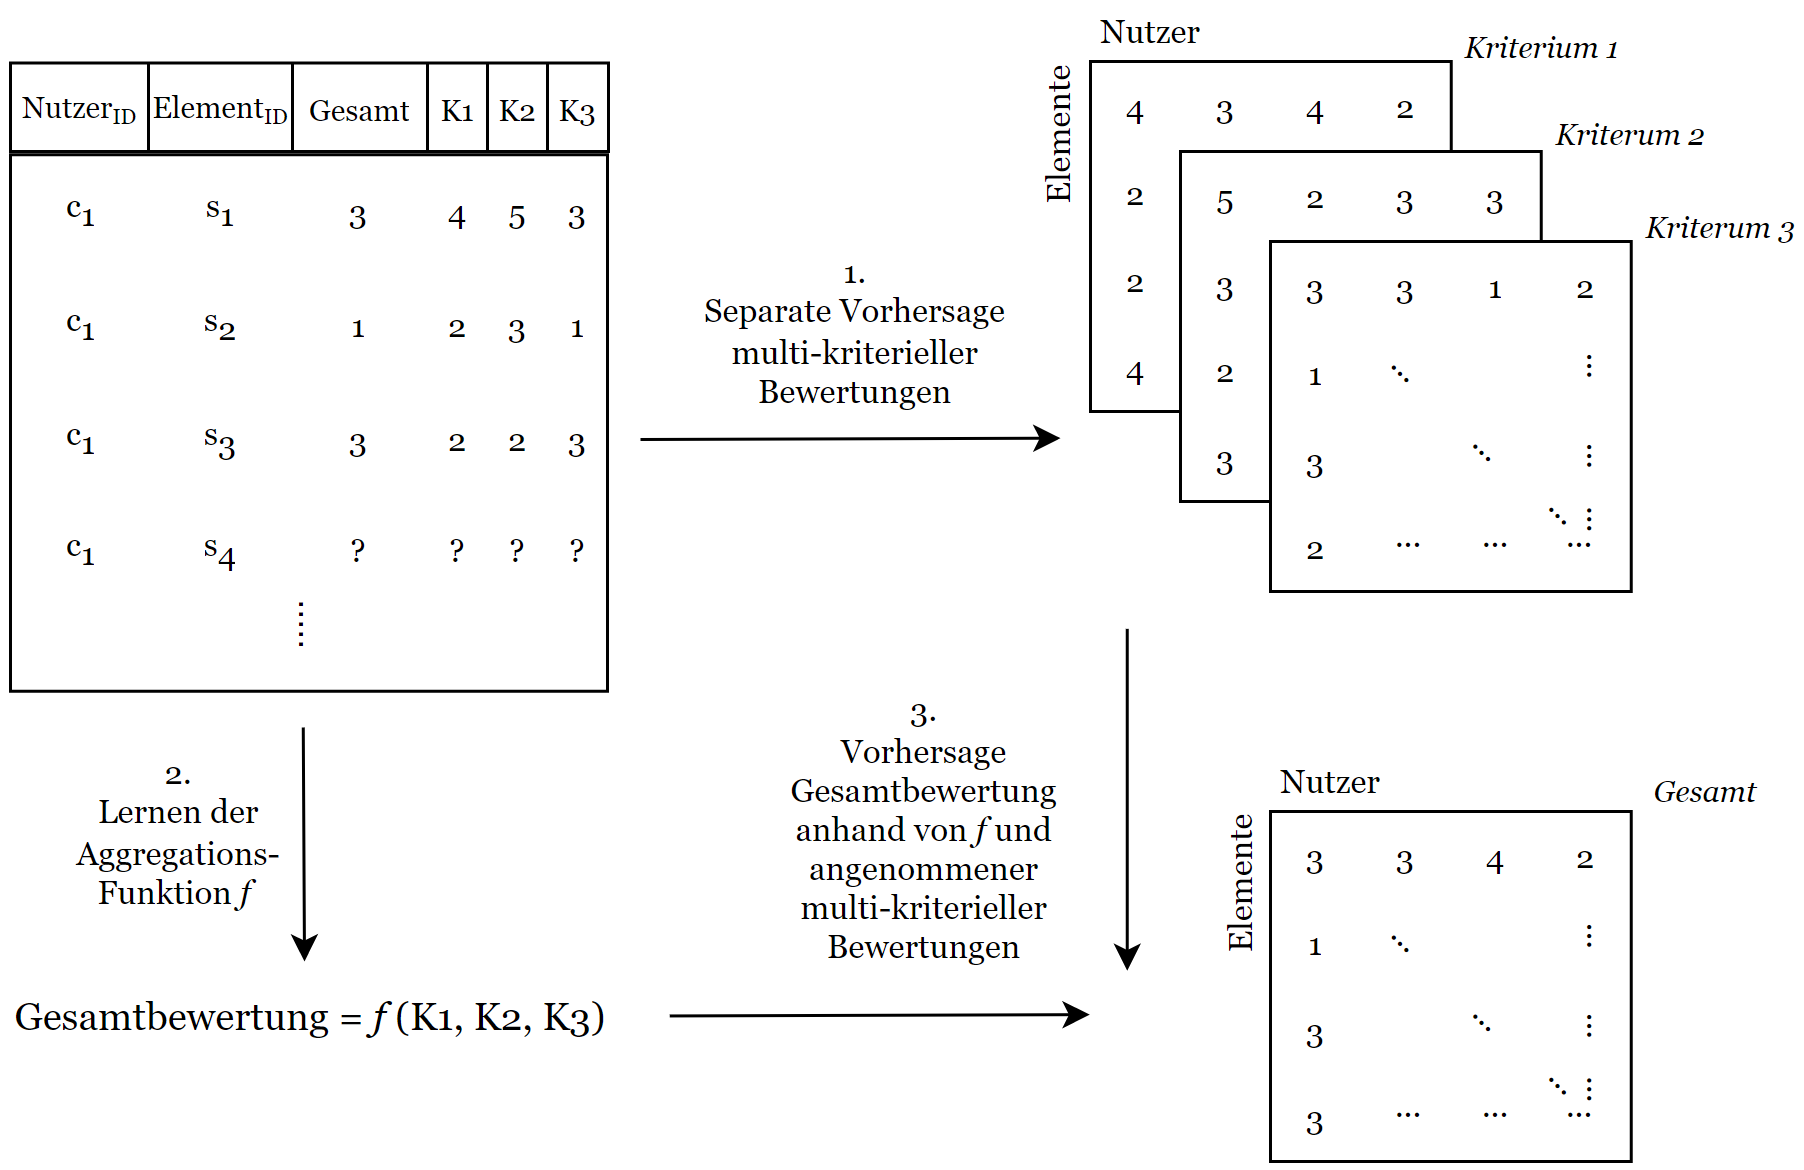
\includegraphics[width=1.0\textwidth]{gfx/a-f-ansatz.png}
	\caption[Aggregation-Function-Ansatz]{Aggregation-Function-Ansatz\\
    (Eigene Darstellung in Anlehnung an \cite[S. 862]{adomavicius:4:inbook})}
	\label{fig:optimierung:loesungen:abb1}
\end{figure}

Im ersten Schritt wird die $k$-dimensionale Rating-Matrix in $k$ unikriterielle Rating-Matrizen der traditionellen Form (Nutzer$\times$Element-Matrix) aufgeteilt \cite[S. 53]{adomavicius:inproceedings:2}.
Für jedes Kriterium $i \in {1,...,k}$ wird daraufhin unter Anwendung eines beliebigen Algorithmus (z.B.: kollaboratives Filtern, inhaltsbasierte Algorithmen) dessen fehlende Bewertungen vorhergesagt \cite[S. 428]{recommenderSystems:2016}.
Dadurch wird das $k$-dimensionale multi-kriterielle Problem in $k$ unikriterielle Probleme zerlegt \cite[S. 861]{adomavicius:4:inbook}.
Schritt 2 umfasst das Aufstellen der Aggregatios-Funktion $f$.
Nach \textcite[S. 53]{adomavicius:inproceedings:2} existieren hierfür maßgeblich drei Verfahren:
\begin{itemize}
    \item \textit{Domänenwissen:} Aufstellen der Funktion basierend auf Erfahrungen und Domänenwissen. Ein simpler Ansatz stellt der Durchschnitt aller angenommenen Bewertungen der einzelnen Kriterien als Aggregations-Funktion dar.
    \item \textit{Statistische Methoden:} Aufstellen der Funktion anhand statistischer Verfahren (z.B. lineare und nicht-lineare Regressionsanalysen) \cite[S. 53]{adomavicius:inproceedings:2}. So kann die Vorhersage einer Gesamtbewertung in der linearen Regression als eine Linearkombination der (angenommenen) multi-kriteriellen Bewertungen repräsentiert werden \cite[S. 429]{recommenderSystems:2016}:
    \begin{equation}\label{eq23}
        \hat{r}^{0} = \sum\limits_{i=1}^{k}w^{i} r^{i}
    \end{equation}
    Die Gewichte $w^{1}, ..., w^{k}$ der Kriterien können anhand verschiedener Techniken der linearen Regression bestimmt werden \cite[S. 429]{recommenderSystems:2016}.
    \item \textit{Techniken des Maschinellen Lernens:} Aufstellen der Funktion über Modelle des Maschinellen Lernens (z.B. neuronale Netze) \cite[S. 53]{adomavicius:inproceedings:2}.
\end{itemize}
Weiter unterscheiden \textcite[S. 53]{adomavicius:inproceedings:2} Aggregations-Funk\-tionen in Abhängigkeit ihres Bezugs.
Wird eine Funktion verwendet um Vorhersagen für alle \ac{N-E-K}-en übergreifend zu treffen, wird diese als total Aggregation-Function bezeichnet (d.h. Gewichte sind nutzer- bzw. elementübergreifend festgesetzt).
Als nutzerbasiert bzw. elementbasiert wird eine Aggregations-Funktion bezeichnet, die basierend auf Bewertungen eines einzelnen Nutzers bzw. Elements bestimmt wird.
Dies kann in Domänen sinnvoll sein, in denen sich die Gewichte einzelner Kriterien zwischen Nutzern bzw. Elementen stark unterscheiden \cite[S. 53]{adomavicius:inproceedings:2}.

Im letzten Schritt erfolgt die Vorhersage der Gesamtbewertungen basierend auf den (angenommenen) multi-kriteriellen Bewertungen und der erstellten Aggregation-Function $f$ \cite[S. 861]{adomavicius:4:inbook}.

Neben dem Aggregation-Function-Ansatz nennen \textcite[S. 861]{adomavicius:4:inbook} probabilistische Modellierungs-Ansätze für die Integration multi-kriterieller Bewertungen in Empfehlungssystemen.
Vereinfacht gesehen handelt es sich dabei um Methoden, die mit Wahrscheinlichkeiten für Bewertungen arbeiten.
\textcite[S. 861]{adomavicius:4:inbook} nennen als Beispiel die Veröffentlichung von \textcite[S. 231]{sahoo:article}.
In der Veröffentlichung wird eine Anpassung des \ac{FMM} von \textcite[S. 704ff.]{si:inproceedings} um multi-krierielle Bewertungen vorgestellt.
\textcite[S. 358]{jin:article} beschreiben das \ac{FMM} als eine grafische Darstellung eines probabilistischen Modells, in dem Nutzer und Elemente (mehreren)\footnote{Das \ac{FMM} unterscheidet sich von herkömmlichen grafischen Modellen unter anderem darin, dass Nutzer bzw. Elemente mehreren Clustern zugeordnet werden können \cite[S. 3]{si:inproceedings}\cite[S. 366]{jin:article}.} Clustern (Klassen) zugeordnet werden können.
Das \ac{FMM} folgt der Annahme, dass eine Bewertung r, welche ein Element s von einem Nutzer c erhält, von einer latenten Variable $Z_{c}$ und einer latenten Variable $Z_{s}$ abhängt \cite[S. 235]{sahoo:article}.
$Z_{c}$ kennzeichnet die Klasse(n), denen ein Nutzer $c$ und ${Z_{s}}$ die Klasse(n), denen ein Element $s$ zugeordnet werden kann \cite[S. 862]{adomavicius:4:inbook}\cite[S. 3]{si:inproceedings}.
Die Wahrscheinlichkeit der Bewertung $r$ eines Nutzers $c$ für ein Element $s$ ergibt sich nach \textcite[S. 862]{adomavicius:4:inbook} aus der Summe aller Wahrscheinlichkeiten der Kombinationen der Variablen $Z_{c}$ und $Z_{s}$:
\begin{equation}\label{eq24}
    P(c,s,r) = \sum\limits_{Z_{c}, Z_{s}}=P(Z_{c})P(Z_{s})P(c|Z_{c})P(s|Z_{s})P(r|Z_{c},Z_{s})
\end{equation}
Das grundlegende Modell ist in Abbildung \ref{fig:optimierung:loesungen:abb2:1} dargestellt, wobei die latenten Variablen grau hinterlegt sind.
% Mixture Models sind grafische Darstellungen probabilistischer Modelle, in denen Nutzer bzw. Elemente in Empfehlungssystemen in Clustern zusammengefasst werden und in Verbindung mit Bewertungen gesetzt werden können.
% Dadurch kann die Ähnlichkeit von Nutzern anhand deren Bewertung eines Element-Clusters erfolgenbasieren und nicht auf Ratings eines einzelnen Elements.
% Mixture Models wurden ursprünglich entwickelt, um das Sparsity-Problem zu umgehen.
% Vereinfacht gesagt ist eine Bewertung r abhängig von einer Nutzerklasse und einer Elementklasse und nicht genau von einem Nutzer und einem Element.

\begin{figure}[H]
    \centering
    \subfloat[Flexible Mixture Model]{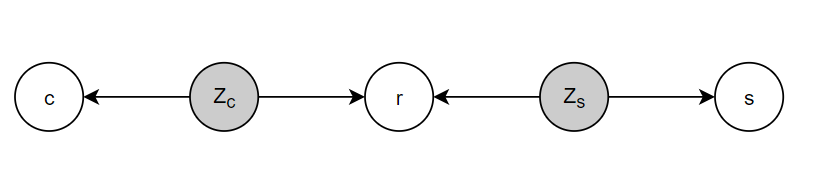
\includegraphics[height=0.9in]{gfx/f-m-m.png}\label{fig:optimierung:loesungen:abb2:1}}\\
    \subfloat[Flexible Mixture Model mit multi-kriteriellen Bewertungen und Dependency-Struktur]{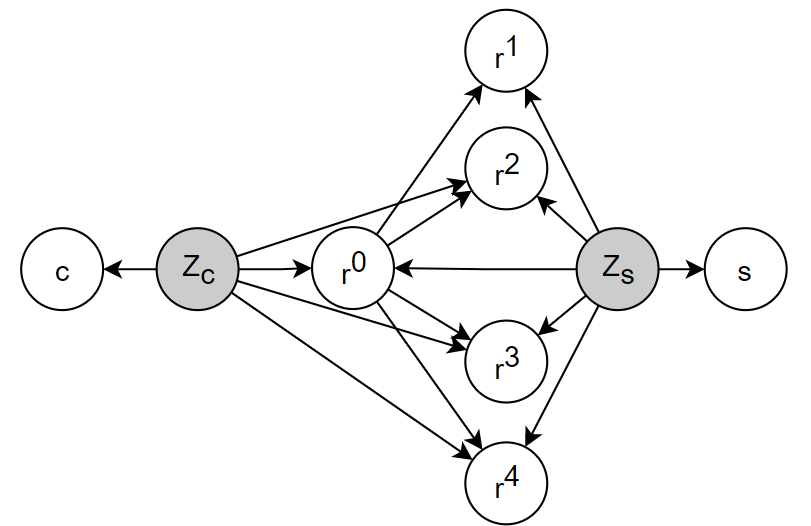
\includegraphics[height=2.20in]{gfx/f-m-m-2.png}\label{fig:optimierung:loesungen:abb2:2}}\\
  \caption[Probabilistischer Modellierungs-Ansatz]{Probabilistischer Modellierungs-Ansatz\\
	(Eigene Darstellung in Anlehnung an \cite[S. 836]{adomavicius:4:inbook})}\label{fig:optimierung:loesungen:abb2}
\end{figure}

\textcite[S. 235]{sahoo:article} erweitern das \ac{FMM} um multi-kriterielle Bewertungen.
Weiter unterstellen \textcite[S. 236f.]{sahoo:article} eine strukturelle Abhängigkeit zwischen den Bewertungen der einzelnen Kriterien (inkl. Gesamtbewertung).
Nach \textcite[S. 236f.]{sahoo:article} besteht die stärkste Abhängigkeit (durchschnittliche Korrelation) zwischen der Gesamtbewertung eines Elements und den Bewertungen der einzelnen Kriterien.
% Das bedeutet, dass nicht jedes Bewertungskriterium gänzlich neue Information über die Präferenzen eines Nutzers liefert, sondern, dass die Gesamtbewertung einen starken Einfluss auf die Ausprägung der Bewertungen der einzelnen Kriterien hat \cite[S. 235]{sahoo:article}.
Die Abhängigkeiten (engl.: Dependency Structure) zwischen den Kriterien bilden \textcite[S. 235]{sahoo:article} in Anlehnung an Dependence Trees von \textcite[S. 463]{chow:article} als Baum ab.
Die Integration multi-kriterieller Bewertungen in das ursprüngliche \ac{FMM} in Form einer der Dependency Structure ist in Abbildung \ref{fig:optimierung:loesungen:abb2:2} grafisch dargestellt.

Die Vorhersage fehlender Bewertungen anhand des Ansatzes erfolgt in zwei Schritten. 
Im ersten Schritt werden die Parameter ($Z_{c}$ und $Z_{s}$ \cite[S. 4]{si:inproceedings}) des \ac{FMM} mithilfe des Expectation Maximization Algorithmus von \textcite[S. 1ff.]{dempster:article} bestimmt \cite[S. 863]{adomavicius:4:inbook}.
Unter Anwendung der Parameter wird darauffolgend der Wert einer fehlenden Bewertung als die Bewertung mit der höchsten Wahrscheinlichkeit vorhergesagt \cite[S. 863]{adomavicius:4:inbook}. 
% HIER WEITERMACHEN mit Erklärung der Vorgehensweise zur Bestimmung fehlender Bewertungen

% Wenn im bereich multi-criteria ratings, dann unterscheiden zwischen vorhandenes overall rating ode rnicht vorhandenes overall rating
% wenn bei overall rating können ansätze aus der allgemeinen multi-kriteriellen optimierung auf RS übertragen werden

\subsection{Pareto-Optimierung}
% Skyline querie siehe Lee and Teng 2007: . Incorporating multi-criteria ratings in recommendation systems.

\subsection{Aggregation}

\subsection{Bedingungen}

\shorthandon{"}
\definecolor{exxetagray}{gray}{0.75}
\definecolor{itemcolor}{RGB}{179,217,255}
\definecolor{usercolor}{RGB}{255,204,179}

\shorthandoff{"}
\chapter{Verwandte Arbeiten}
\label{ch:verwandte_arbeiten}


\section{Reziproke Systeme}

\subsection{Systeme mit identischer Gewichtung der Präferenzen}
% d.h. wie sehr zwei personen übereinstimmen, beides gleich gewichtet
% Dual perspektive graph representation hier: S. 104, file://wsl%24/Ubuntu/home/masc6/Projects/masterarbeit/literatur/recsys%202022%20modeling%20two%20way%20selection%20preference%20for%20person%20job%20fit.pdf

\subsection{Systeme mit unterschiedlicher Gewichtung der Präferenzen}
% präferenz eines nutzers höher gewichtet als präferenz der empfohlenen Elemente
% feature optionen können 3 unterschiedliche stadi annehmen. -> classification (label mit match und kein match) S. 68, file://wsl%24/Ubuntu/home/masc6/Projects/masterarbeit/literatur/DiazMetzlerAmer-Yahia%20-%20Relevance%20and%20Ranking%20in%20Online%20Dating%20Systems%20(2010)%20-%200.pdf
% Johannes Thesis

\section{Multi-kriterielle Systeme}
hier bsp anführen für arbeiten die sich mit mk systemen beschäftigen in den 3 bereichen
% Hier erwähnen, dass nicht alle systeme auch als mk-systeme bezeichnet sind, die solche Ansätze anwenden (bspw. hybride systeme)
% Hier erwähnen, dass Fokus auf aggregation mehrerer Kriterien und deren gewichtung liegt -> hiernach suchen

% Verwendung von MAUT (siehe S. 432, file://wsl%24/Ubuntu/home/masc6/Projects/masterarbeit/literatur/Analysis%20and%20Classification%20of%20Multi-Criteria.pdf)
% MAUT in utility based recommenders: file://wsl%24/Ubuntu/home/masc6/Projects/masterarbeit/literatur/Designing%20utility-based%20recommender%20systems%20for%20e-commerce.pdf

\subsection{Multi-attribut basierte Systeme}
% hybrid recommender: weighted -> S. 339, https://link.springer.com/content/pdf/10.1023/A:1021240730564.pdf?pdf=button

\subsection{Multi-objektive Systeme}
% multi-objective example: S. 237, file://wsl%24/Ubuntu/home/masc6/Projects/masterarbeit/literatur/Adaptive%20multi%20attribute%20diversity%20for%20recommender%20systems.pdf

\subsection{Multi-kriterielle Bewertungen in Empfehlungssystemen}
% Erfinder des aggregation Funktion approaches: file://wsl%24/Ubuntu/home/masc6/Projects/masterarbeit/literatur/New_Recommendation_Techniques_for_Multicriteria_Rating_Systems.pdf
% Arbeit von Jannach wie hier beschrieben mit SVM: S. 102, file://wsl%24/Ubuntu/home/masc6/Projects/masterarbeit/literatur/E-Commerce.pdf
% multi-kriteria: Aggregation function approach: file://wsl%24/Ubuntu/home/masc6/Projects/masterarbeit/literatur/Recommending%20Hotels%20based%20on%20Multidimesional%20Customer%20Ratings.pdf
% ansatz von Tang: zusammenfügen mehrere feature bewertungen, sowie durchschnittsbewertung und kommentare, file:///C:/Users/masc6/Downloads/tdladmin,+TangandMcCalla_JoDI_final.pdf
% Slope one algorithmus und adaptive genetic algorithm von Hassan, S. 327, file://wsl%24/Ubuntu/home/masc6/Projects/masterarbeit/literatur/Imrpoving%20Prediction%20accuracy%20of%20multi-criteria%20recommender.pdf
% Liu et al.: Cluster von Nutzern, welche wichtigkeit einzelner Attribute angeben, zusammenfassung siehe hier S. 4, file:///C:/Users/masc6/Downloads/79_HDIOUD.pdf
% CCSD method, siehe: file:///C:/Users/masc6/Downloads/79_HDIOUD.pdf
% Wenn viele features: liwei et al (zsfsg. siehe hier: file://wsl%24/Ubuntu/home/masc6/Projects/masterarbeit/literatur/A%20Multi-criteria%20Recommender%20System%20Incorporating%20Intensity%20of%20Preferences.pdf )

% was gibt es also nicht? -> Reziprozität als gewichtetes Kriterium (Präferenz der empfohlenen Person zählt nicht genauso viel wie Präferenz des Nutzers, kann daher als gewichtetes Kriterium einer Aggregation Function betrachtet werden, welche über historische daten erlernt werden kann)
% Neue anwendungsbereiche von multi-kriteriellen EMpfehlungen in domänen wie online dating: zitat von 
\shorthandon{"}
\shorthandoff{"}
\chapter{Methodik}
\label{ch:methodik}

\section{Art der Forschung}
\label{ch:methodik:art}
Um die Forschungsfrage dieser Master-Thesis zu untersuchen, wird eine quantitative Forschungsarbeit in Form eines Experiments durchgeführt. In diesem Kontext werden für einen A/B-Test zwei Versionen eines Empfehlungssystems zur Besetzung offener Projektpositionen entwickelt. Eine der beiden Anwendungen soll einen unilateralen, die andere einen bilateralen Ansatz verfolgen. Beide Empfehlungssysteme erhalten als Eingabe dieselben offenen Projektpositionen. Für diese Stellen sortieren die Anwendungen die vorhandenen Mitarbeiter eines Betriebs und geben diese in Form einer Liste zurück.

Die Ausgaben beider Systeme werden Projektmanagern des Unternehmens vorgelegt. Diese bewerten auf einer vordefinierten Skala, welche Arbeitsleistung sie von denen in der vorliegenden Reihenfolge dargestellten Mitarbeitern erwarten.

Die Angestellten erhalten die Beschreibungen der offenen Projektpositionen und bewerten ebenfalls auf einer vordefinierten Skala, wie zufrieden sie voraussichtlich mit der Tätigkeit auf den vorliegenden Projektpositionen sein werden. Hierbei wird für beide Empfehlungssysteme überprüft, ob eine hohe erwartete Zufriedenheit der Angestellten mit einer hohen Positionierung in den Ergebnislisten korreliert.

Abschließend werden die Bewertungen von Projektmanagern und Angestellten hinsichtlich der Ergebnisse der beiden Empfehlungssysteme verglichen. Hierbei wird bestimmt, ob die Resultate der bilateralen Recommender Engine im direkten Vergleich mit dem unilateralen Ansatz sowohl auf Seiten der Projektmanager eine höhere erwartete Leistung als auch aus Perspektive der Mitarbeiter für eine höhere erwartete Zufriedenheit sorgt.

\section{Versuchsaufbau}
\label{ch:methodik:versuchsaufbau}
Durchgeführt wird das Experiment mit Projektmanagern und Mitarbeitern der EXXETA AG mit Hauptsitz in Karlsruhe. Das Unternehmen ist spezialisiert auf IT-Beratungsleistungen und arbeitet vorrangig projektbasiert. Passende Angestellte zu offenen Projektpositionen zuzuordnen ist in diesem Betrieb dementsprechend eine häufig auftretende Aufgabe. Daher liegen Informationen über die Kompetenzen der Mitarbeiter bereits in einer strukturieren Form vor.

Die Mitarbeiter der EXXETA AG pflegen ihre Kompetenzen in einem Intranet. Dort steht eine Liste mit 551 Fähigkeiten wie beispielsweise "Java", "DSGVO" und "Digitale Transformation" zur Verfügung. Diese können die Angestellten über die in Abbildung \ref{fig:methodik:versuchsaufbau:daten:abb1} dargestellte Skala bewerten.

\begin{figure}[h]
	\centering
	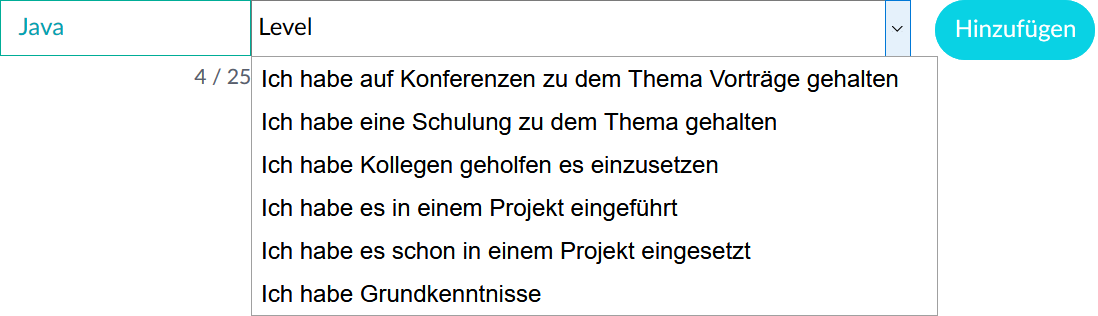
\includegraphics[width=1\textwidth]{gfx/skill-level.png}
	\caption{Hinzufügen einer Fähigkeit mit Angabe des entsprechenden Kenntnisniveaus im EXXETA-Intranet}
	\label{fig:methodik:versuchsaufbau:daten:abb1}
\end{figure}

Die in Abbildung \ref{fig:methodik:versuchsaufbau:daten:abb1} dargestellten Abstufungen werden beim Speichern in ganzzahlige Werte von null ("Ich habe Grundkenntnisse") bis sechs ("Ich habe auf Konferenzen zu dem Thema Vorträge gehalten") übertragen.

Aufgrund dieser klaren Beschreibungen der einzelnen Stufen in Abbildung \ref{fig:methodik:versuchsaufbau:daten:abb1} kann Bias bei der Selbsteinschätzung weitgehend ausgeschlossen werden. Außerdem ist es in der vorliegenden Problemstellung gut möglich, dass einzelne Mitarbeiter ihre Kompetenzen grundsätzlich besser oder schlechter einschätzen als andere Kollegen. Dieser Sachverhalt kann insbesondere auf längere Berufserfahrung zurückgeführt werden. Daher wird bei der Empfehlungsbestimmung auf eine Mittelwert-Zentrierung verzichtet.

Die Kompetenzen der Mitarbeiter und die zugehörigen Bewertungen dienen im Experiment als Eingabe für das unilaterale Empfehlungssystem.

\subsection{Unilaterales Empfehlungssystem}
\label{ch:methodik:versuchsaufbau:unilateral}
Um im unilateralen Empfehlungssystem Mitarbeiter für offene Projektpositionen vorzuschlagen, wird die Katz-Zentralität angewendet. Dieser speicherbasierte Graphenalgorithmus wurde in Kapitel \ref{ch:empfehlungssysteme:cf:speicherbasiert} vorgestellt. Ein Nutzen dieses Ansatzes ist die zuverlässige Lösung des Sparsity Problems. Vorteilhaft gegenüber modellbasierten Methoden ist außerdem die Langlebigkeit des Verfahrens. Sollten sich nach Durchführung des Experiments Daten im Unternehmen signifikant verändern oder neue Kompetenzen im Intranet hinzugefügt werden, ist der speicherbasierte Ansatz weiterhin unverändert anwendbar. Die dabei zu erwartende hohe Komplexität ist in der vorliegenden Problemstellung tolerierbar, da sich zum Zeitpunkt des Experiments unter 1.000 Mitarbeiter im Unternehmen befinden.

Um neben dem Sparsity Problem auch den Kaltstart zu beheben, werden zusätzlich zu den Fähigkeiten der Mitarbeiter auch deren Teamzuordnungen in Form eines hybriden Ansatzes beachtet. Bei der EXXETA AG arbeiten stets Mitarbeiter in einem Team, welche ähnliche Kompetenzen beherrschen. Der Leiter des Teams ist eine fachliche Führungskraft, dessen Fähigkeiten in der Regel repräsentativ für sein Team sind. Seine Kompetenzen sind jedoch stärker ausgeprägt. Um Rechenleistung einzusparen, werden die Teams nicht als zusätzliche Knoten in den Graphen eingefügt. Die Beziehungen werden stattdessen über direkte Kanten zwischen Kollegen dargestellt. Das Kantengewicht von Teammitglieder zu Teammitglied beträgt eins und das Gewicht von Teammitglied zu seinem Manager zwei. Über diesen Ansatz sind alle Teammitglieder schwach miteinander verbunden, sodass auch für Mitarbeiter ohne vergebene Bewertungen aussagekräftige Beurteilungen bestimmt werden können. Außerdem erhalten die Teammanager durch das höhere Kantengewicht eine stärkere Zentralität im Graphen.  Daher profitieren sämtliche Teammitglieder transitiv von den hinterlegten Fähigkeiten ihres Managers.

Die Fähigkeitsbewertungen und Teamzuordnungen können für alle Mitarbeiter der EXXETA AG über eine \acsu{REST}-Schnittstelle in Form von \acsu{JSON} aus dem Intranet abgefragt werden. Quellcode \ref{qc:methodik:versuchsaufbau:daten:qc1} zeigt beispielhaft einen Auszug aus den zurückgegebenen Daten von John Doe aus Tabelle \ref{tbl:empfehlungssysteme:arbeitsweise:tbl1}.

%\begin{minipage}{\linewidth}
	\lstinputlisting[
	language=json,
	caption=Beispiel für ein Mitarbeiter-\acsu{JSON} der \acsu{REST}-Schnittstelle des Intranets der EXXETA AG (Auszug),
	captionpos=b,
	label=qc:methodik:versuchsaufbau:daten:qc1
	]{gfx/john.json}
%\end{minipage}

In Quellcode \ref{qc:methodik:versuchsaufbau:daten:qc1} ist zu erkennen, dass eine Bewertung von eins in Tabelle \ref{tbl:empfehlungssysteme:arbeitsweise:tbl1} einer Beurteilung von null im zurückgegebenen \ac{JSON} entspricht. Damit ein Kantengewicht von null ausschließlich nicht vergebene Kompetenz-Einschätzungen symbolisiert, werden die Bewertungen vor Berechnung der Katz-Zentralität um eins erhöht.

Abbildung \ref{fig:methodik:versuchsaufbau:unilateral:abb1} zeigt die Darstellung der Kompetenzen und Teamzuordnungen der Mitarbeiter aus Tabelle \ref{tbl:empfehlungssysteme:arbeitsweise:tbl1} in der Form eines bipartiten Graphen. In der Grafik wird Jane Doe als Teammanager betrachtet.

\begin{figure}[h]
	\centering	
	\begin{tikzpicture}[node distance={32mm}, thick, main/.style = {draw, circle}] 
		\node[main, fill=itemcolor] (MongoDB) {$MongoDB$}; 
		\node[main, fill=itemcolor] (Python) [below right of=MongoDB] {$Python$}; 
		\node[main, fill=itemcolor] (MySQL) [above right of=Python] {$MySQL$}; 
		\node[main, fill=itemcolor] (Java) [below right of=MySQL] {$Java$}; 
		\node[main, fill=itemcolor] (HDFS) [above right of=Java] {$HDFS$}; 
		\node[main, fill=itemcolor] (Spark) [below right of=HDFS] {$Spark$};
		
		\node[main, fill=usercolor] (Jane) [above right of=MongoDB] {$Jane D.$}; 
		\node[main, fill=usercolor] (John) [above left of=HDFS] {$John D.$}; 
		\node[main, fill=usercolor] (Max) [below of=MySQL] {$Max M.$};
		\node[main, fill=usercolor] (Erika) [above right of=HDFS] {$Erika M.$}; 
		
		\draw (Jane) -- node[midway, right] {4} (Python);
		\draw (Jane) -- node[midway, above] {3} (MySQL);
		\draw (Jane) -- node[midway, above] {3} (MongoDB);
		
		\draw (John) -- node[midway, right] {1} (HDFS);		
		\draw (John) -- node[midway, right] {3} (Java);
		\draw (John) -- node[midway, above] {2} (MySQL);
		
		\draw (Erika) -- node[midway, above] {5} (HDFS);
		\draw (Erika) -- node[midway, left] {3} (Spark);
		
		\draw (Max) -- node[midway, above] {2} (Java);
		\draw (Max) -- node[midway, above] {3} (Python);
		\draw (Max) -- node[midway, right] {1} (MySQL);
		
		\draw (Jane) -- node[midway, above] {2} (John);
		\draw (Jane) -- node[midway, left] {2} (Max);
		\path (Jane) edge[bend left=25] node[midway, above] {2} (Erika);
		
		\draw (John) -- node[midway, right] {1} (Max);
		\draw (John) -- node[midway, above] {1} (Erika);
		
		\path (Max) edge[bend right=40] node[midway, below] {1} (Erika);
	\end{tikzpicture}
	
	\caption{Graph aus Abbildung \ref{fig:empfehlungssysteme:cf:speicherbasiert:abb2} mit zusätzlicher Teamzuordnung}
	\label{fig:methodik:versuchsaufbau:unilateral:abb1}
\end{figure}

Zur Anwendung des unilateralen Empfehlungssystems gibt ein Projektmanager die für eine offene Projektposition relevanten Fähigkeiten mitsamt des benötigten Kompetenzniveaus in das System ein. Diese Daten werden wie in Kapitel \ref{ch:empfehlungssysteme:cf:speicherbasiert} im Kontext der Gruppen-Recommender Engines beschrieben, in Form eines Pseudo-Mitarbeiters ebenfalls in den bipartiten Graphen aus Abbildung \ref{fig:methodik:versuchsaufbau:unilateral:abb1} eingefügt. Anhand dieser Daten folgt die Bestimmung der Katz-Zentralität. Anschließend wird für jede vom Projektmanager geforderte Kompetenz die absolute Differenz zwischen Pseudomitarbeiter und allen anderen Angestellten bestimmt. Im letzten Schritt werden die Mitarbeiter nach geringster Abweichung sortiert und an den Projektmanager zurückgegeben.

\subsection{Bilaterales Empfehlungssystem}
\label{ch:methodik:versuchsaufbau:bilateral}

\newpage
Zu erhebende Daten:\\
- Für jeden Mitarbeiter erheben: Wichtigkeit (true/false) --> Auch für Dinge, die man noch nicht kann\\
- Für jeden Mitarbeiter erheben: Welche Auswirkung hat es, wenn im Projekt nicht ausgelastet (Kurve A bis C) --> Alle drei Antwortmöglichkeiten positiv formulieren --> z.B. Freiräume nutzen

Erstellen des Graphen:\\
- Aus Skills (kollaboratives Filtern) und Teamzuordnung (Inhaltsbasiertes Filtern) einen tripartiten Graphen erstellen\\

Eingabe der offenen Projektposition:\\
- Benötigt: Fähigkeiten und Wichtigkeit (Boolean)

Algorithmus:\\
- Berechnung der Katz-Zentralität\\
- Für jeden relevanten Mitarbeiter auf Basis von Abbildung \ref{fig:methodik:abb2} den finalen Wert bestimmen --> Hierbei je nach Wichtigkeit die Kurve stauchen --> Wenn für Projektmanger wichtig, die durchgezogene Linie doppelt so steil; Wenn für Mitarbeiter wichtig, rechte Seite doppelt so steil; Auswahl der Kurve anhand der Information des Mitarbeiters\\
- Summe für alle Fähigkeiten eines Projektes für jeden Mitarbeiter berechnen

\begin{figure}[h]
	\centering
	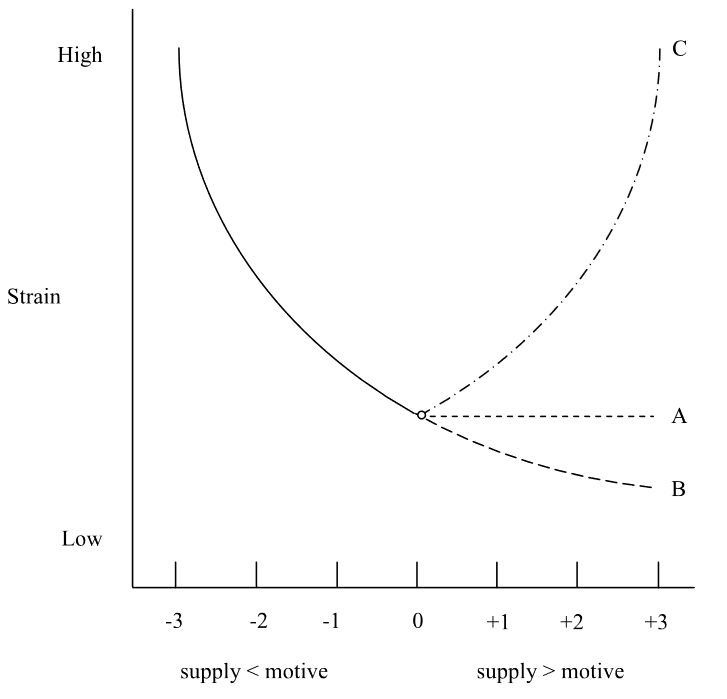
\includegraphics[width=0.75\textwidth]{gfx/ueberschuss_supply_motive.png}
	\caption{Auswirkungen eines Bedürfnisse-Angebote Misfits \cite[S. 23]{edwards:2008}\\(Bearbeitet von \myName)}
	\label{fig:methodik:abb2}
\end{figure}

- Algorithmus einmal durchführen mit Wichtigkeiten und einmal ohne (bilateral vs. unilateral)\\
- Ausgabe der sortierten Liste (mit allen Mitarbeitern (zB 25))\\
- Eingabe der Projektposition und Algorithmus für jede Projektposition wiederholen

\section{Geplante Evaluation}
\label{ch:methodik:evaluation}
Evaluation für Projektmanager:\\
- Erhält für jedes Projekt beide Listen und gibt auf einer Skala von 1 bis 5 an, wie hoch der die Leistung der empfohlenen Mitarbeiter in diesem Projekt einschätzen würde

Evaluation für Mitarbeiter:\\
- Jeder Mitarbeiter muss für jedes Projekt auf einer Skala von 1 bis 5 bewerten, wie zufrieden er wäre, wenn er darin arbeiten würde\\
- Ergebnisliste wird in Intervalle geteilt --> z.B. Zufriedenheit 5 bedeutet bei 25 Teilnehmern, dass der Nutzer im ersten Intervall sein muss --> Abweichung bestimmen --> Je weniger Abweichung, desto besser --> Durchschnittliche Abweichung von unilateral und bilateral vergleichen

Frage:\\
- Sollte Manager überhaupt Wichtigkeiten angeben?\\
	- Fähigkeiten sind Angebote und Wichtigkeiten Nachfrage\\
- Ist das Vergleichs-Vorgehen unilateral?\\
- Welche Daten müssen in den Anhang der Thesis?
\shorthandon{"}

\shorthandoff{"}
\chapter{Forschungsergebnisse}
\label{ch:ergebnisse}

\section{Analyse von Fähigkeiten und Präferenzen}
\label{ch:ergebnisse:analyse}

\subsection{Fähigkeiten der Mitarbeiter aus dem Intranet}
\label{ch:ergebnisse:analyse:faehigkeiten}
An der Umfrage unter den Projektmitarbeitern haben N=23 Personen aus dem Fachbereich \acl{JES} der EXXETA AG teilgenommen. Diese Angestellten haben insgesamt 643 Kompetenzbewertungen im Intranet des Unternehmens abgegeben. Dies entspricht ca. 28 vergebenen Beurteilungen pro Person. Die Bewertungen verteilen sich auf 212 der \anzFaehigkeiten unterschiedlichen, im Intranet gespeicherten Fähigkeiten. Java ist mit 16 Beurteilungen die meist beherrschte Kompetenz.

Abbildung \ref{fig:ergebnisse:analyse:abb1} zeigt die im Intranet bewerteten Fähigkeiten sortiert nach Anzahl an Beurteilungen. Dabei ist der in Kapitel \ref{ch:empfehlungssysteme:cf:speicherbasiert} vorgestellte lange (Ratten-)Schwanz gut erkennbar. Dieser ist jedoch weniger stark ausgeprägt, als in der Referenzdarstellung aus Abbildung \ref{fig:empfehlungssysteme:cf:speicherbasiert:abb1}.

\begin{figure}[h]
	\centering
	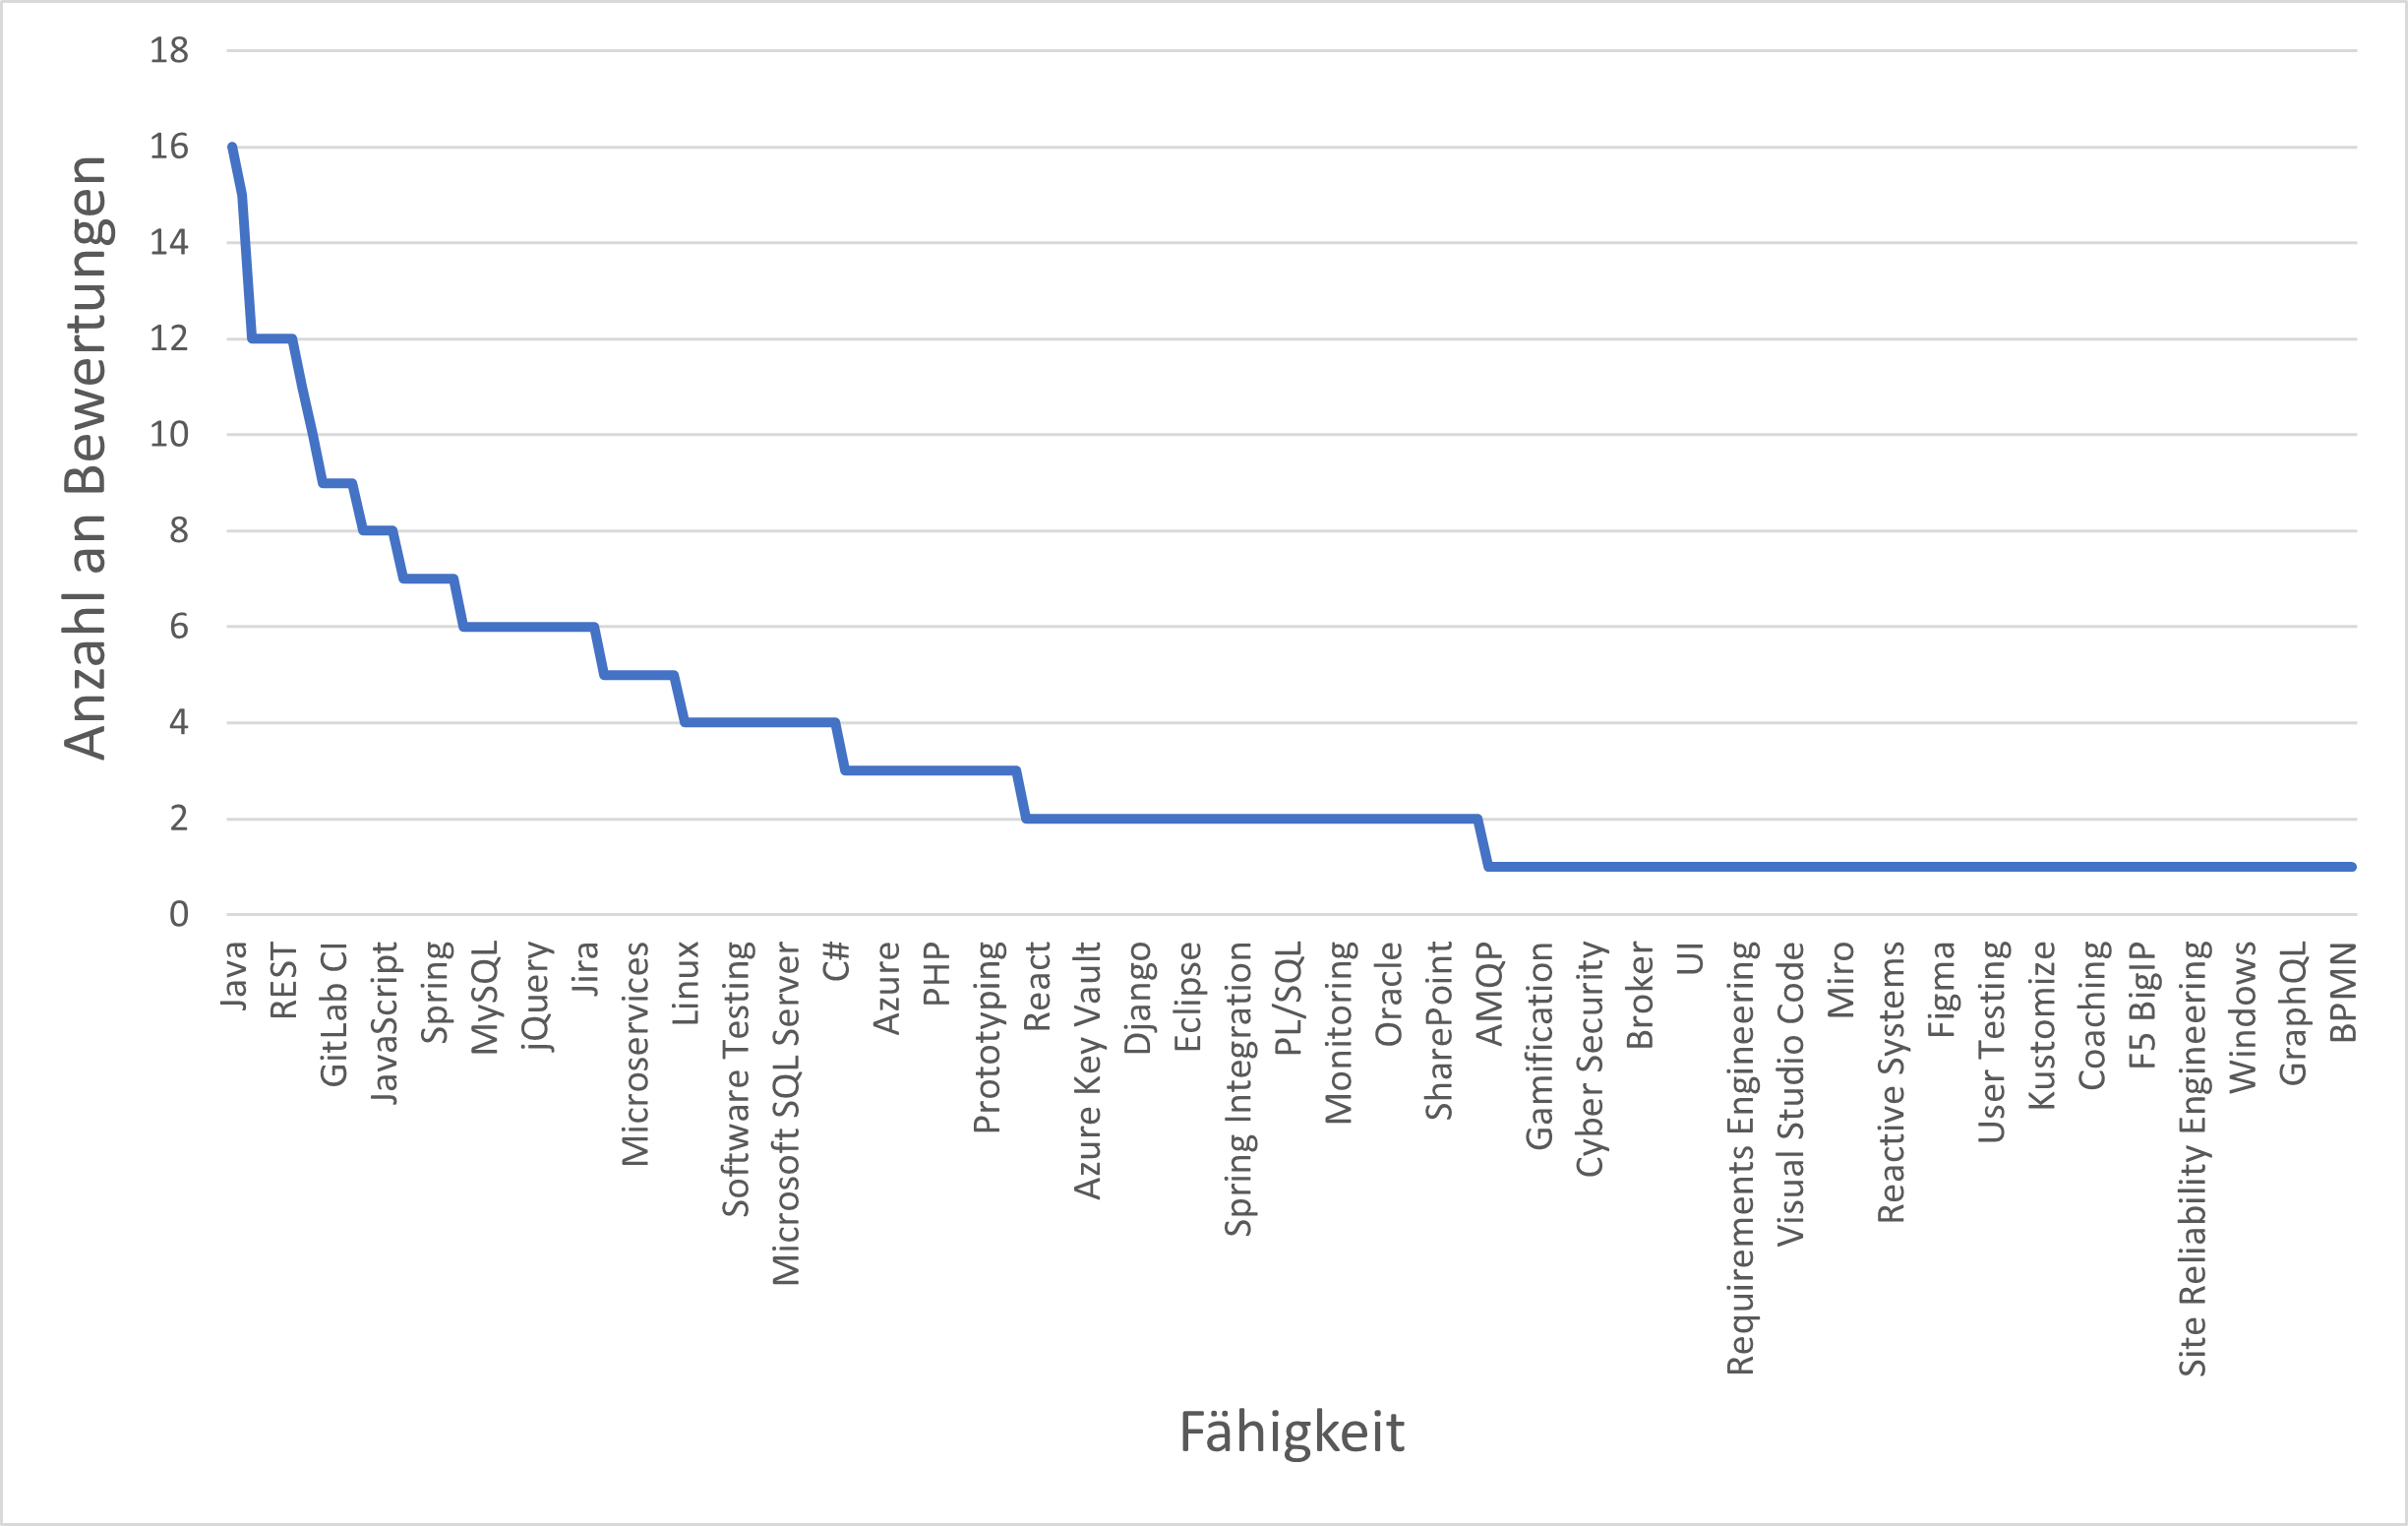
\includegraphics[width=1\textwidth]{gfx/long-tail-intranet.png}
	\caption{Langer (Ratten-)Schwanz bei den Fähigkeitsbewertungen im EXXETA-Intranet}
	\label{fig:ergebnisse:analyse:abb1}
\end{figure}

In Abbildung \ref{fig:ergebnisse:analyse:abb1} ist bezüglich des langen (Ratten-)Schwanzes festzustellen, dass neun bzw. etwa 4.3 Prozent aller Fähigkeiten über zehn oder mehr Bewertungen verfügen. Dagegen haben 151 bzw. etwa 71.2 Prozent aller Kompetenzen drei oder weniger Beurteilungen.

In den vorliegenden Daten des Intranets ist darüber hinaus zu beobachten, dass vier bzw. etwa 17.4 Prozent der Mitarbeiter keine einzige Fähigkeit bewertet haben. Diese Angestellten sind seit Einführung des Kompetenz-Bewertungssystems durchgehend in einem Projekt tätig und daher von ihrer Führungskraft noch nicht zur Pflege ihrer Fähigkeiten aufgefordert worden.

\subsection{Präferenzen der Mitarbeiter aus der Umfrage}
\label{ch:ergebnisse:analyse:praeferenzen}
Bei der Umfrage zu den Präferenzen haben die Mitarbeiter insgesamt 1408 Bewertungen abgegeben, welche sich auf 370 einzelne Kompetenzen verteilen. Dies entspricht knapp über 61 abgegebenen Wünschen pro Mitarbeiter. Git ist mit 18 Beurteilungen die meist präferierte Fähigkeit. Wie in Abbildung \ref{fig:ergebnisse:analyse:abb2} zu erkennen, deutet sich auch hinsichtlich der Wünsche ein langer (Ratten-)Schwanz an, wenn die Fähigkeiten nach Anzahl an Beurteilungen sortiert dargestellt werden.
 
\begin{figure}[h]
	\centering
	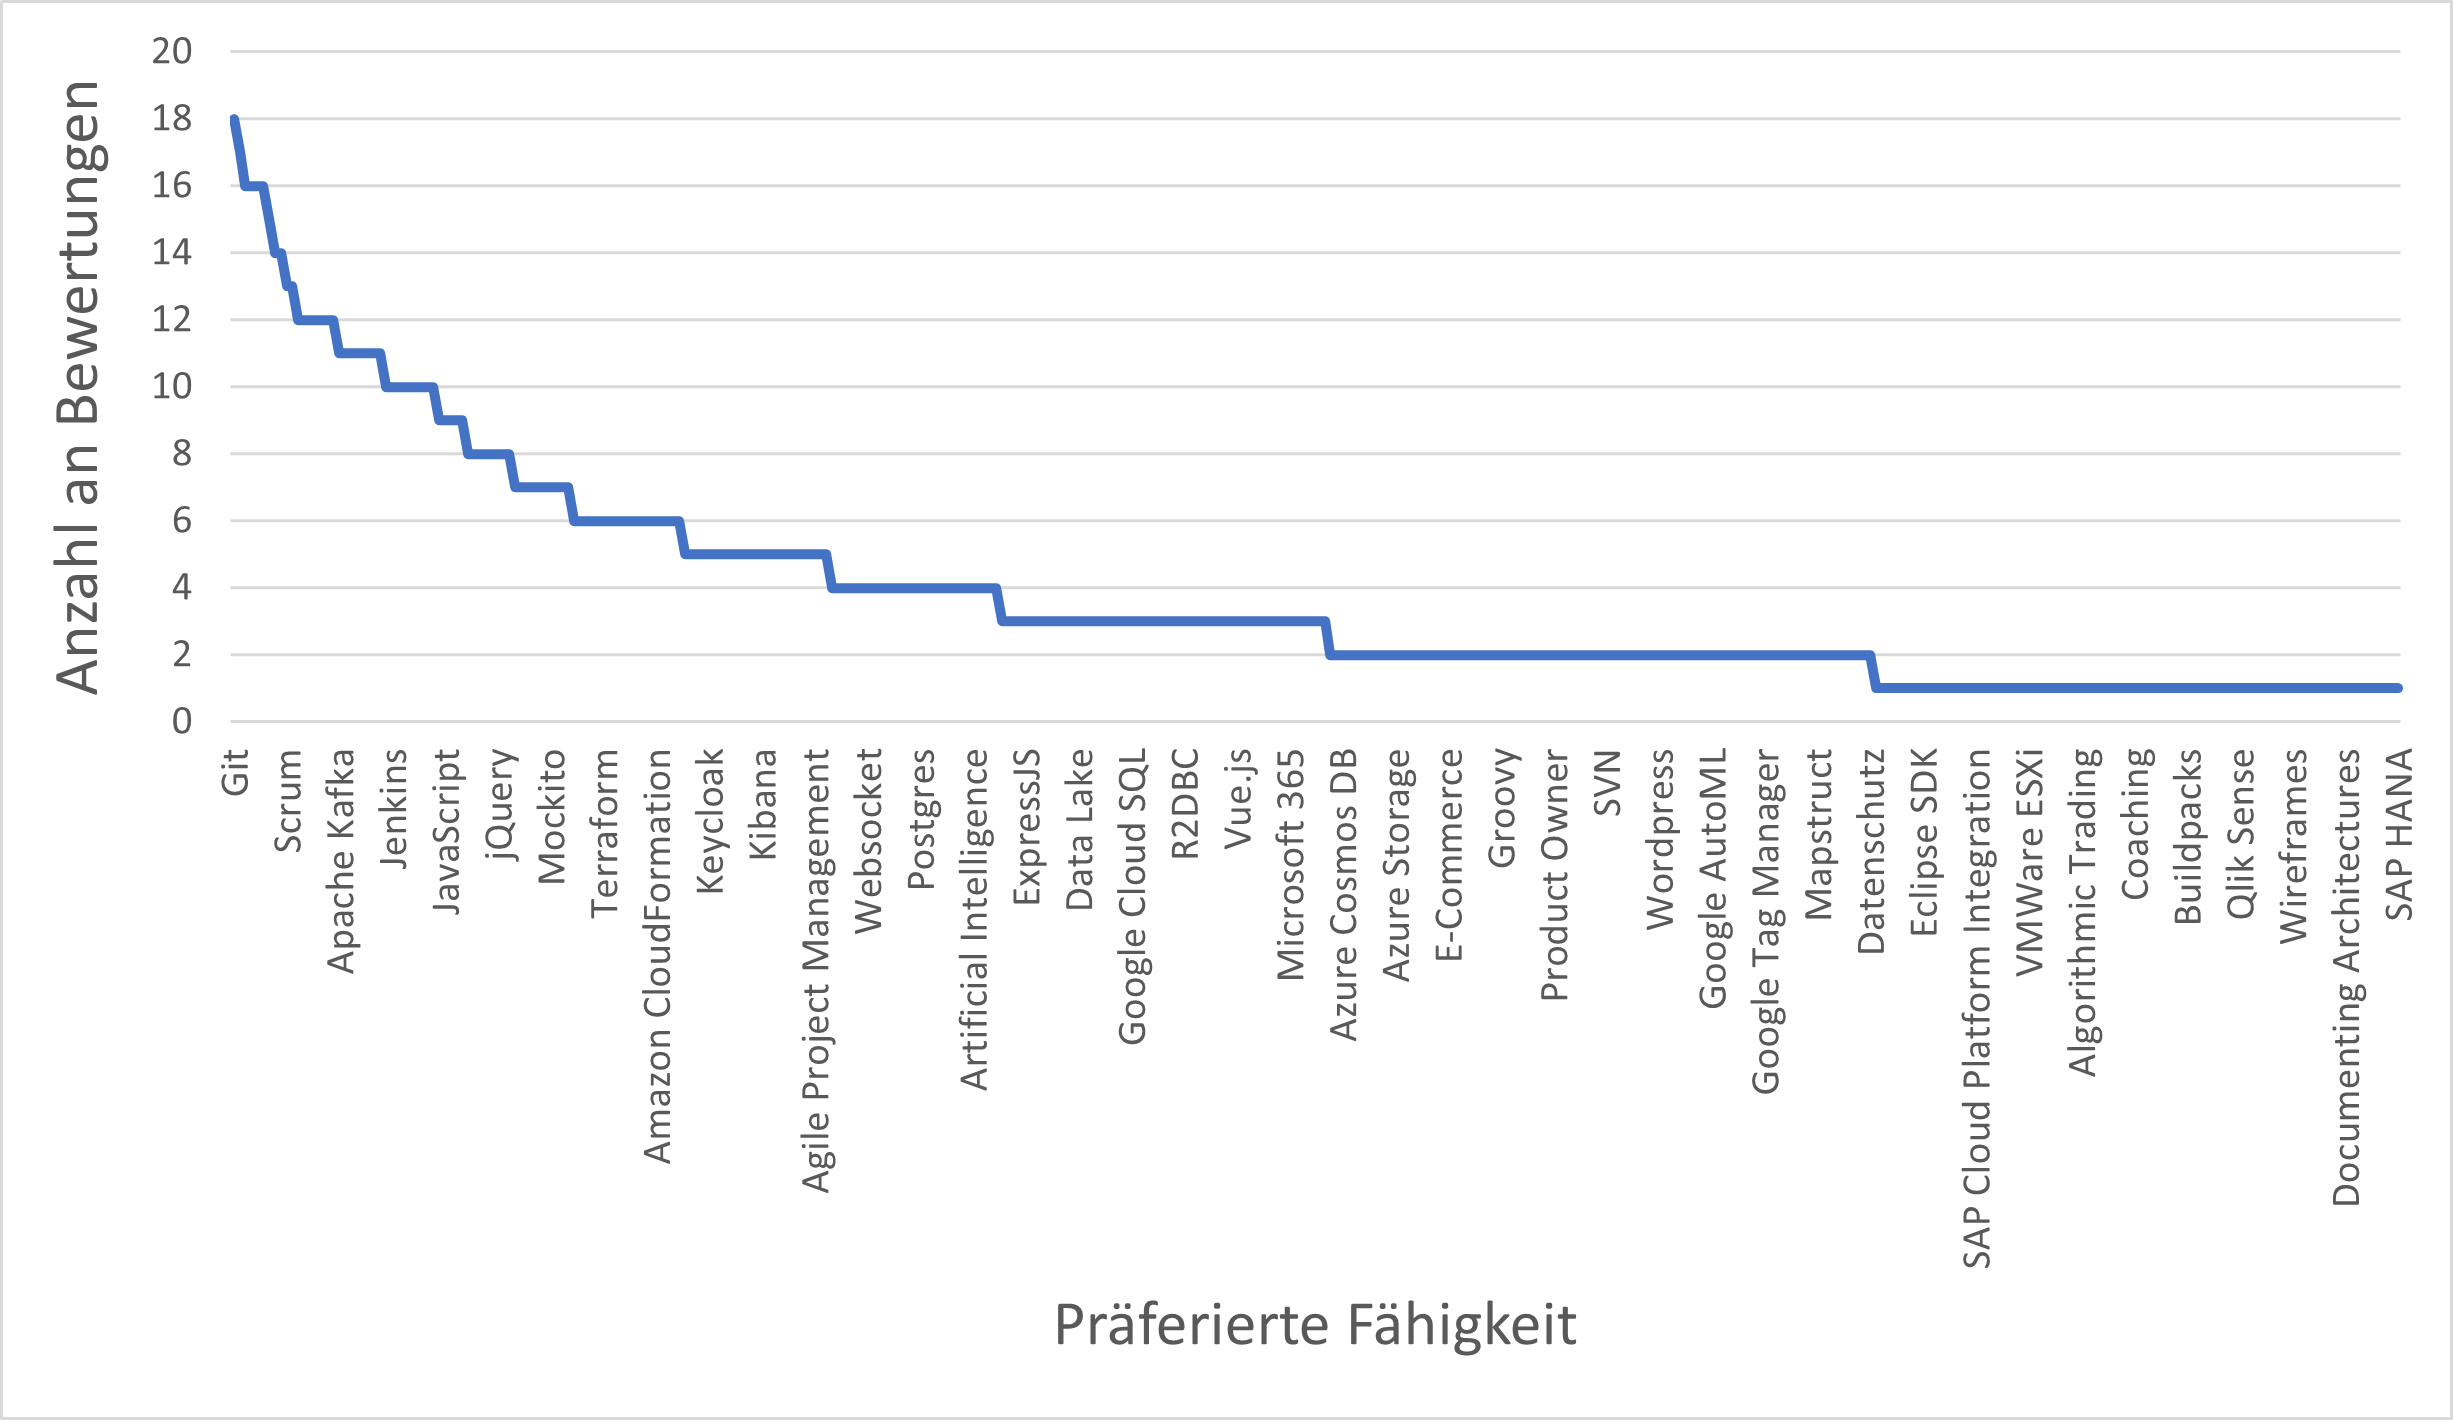
\includegraphics[width=1\textwidth]{gfx/long-tail-praeferenzen.png}
	\caption{Langer (Ratten-)Schwanz bei den präferierten Fähigkeiten der Mitarbeiter}
	\label{fig:ergebnisse:analyse:abb2}
\end{figure}

Zu Abbildung \ref{fig:ergebnisse:analyse:abb2} ist festzustellen, dass 18 bzw. etwa 4.9 Prozent aller Fähigkeiten von zwölf oder mehr Mitarbeitern präferiert werden. Dem gegenüber stehen 268 bzw. etwa 72.4 Prozent aller Kompetenzen, welche vier oder weniger Angestellte als Wunsch angegeben haben. Bei der Umfrage gab es keinen Mitarbeiter, welcher keine einzige Fähigkeit als Präferenz ausgewählte.

\subsection{Gemeinsame Betrachtung beherrschter und präferierter Fähigkeiten}
\label{ch:ergebnisse:analyse:gemeinsam}
Bei der gemeinsamen Betrachtung von Kompetenzen und Wünschen ist auf Mitarbeiterebene festzustellen, dass ein durchschnittlicher Angestellter etwa 74.7 Fähigkeiten beherrscht und/oder präferiert. Abbildung \ref{fig:ergebnisse:analyse:abb3} zeigt, wie viele dieser Kompetenzen der durchschnittliche Mitarbeiter beherrscht und wie viele er davon präferiert.

\begin{figure}[h]
	\centering
	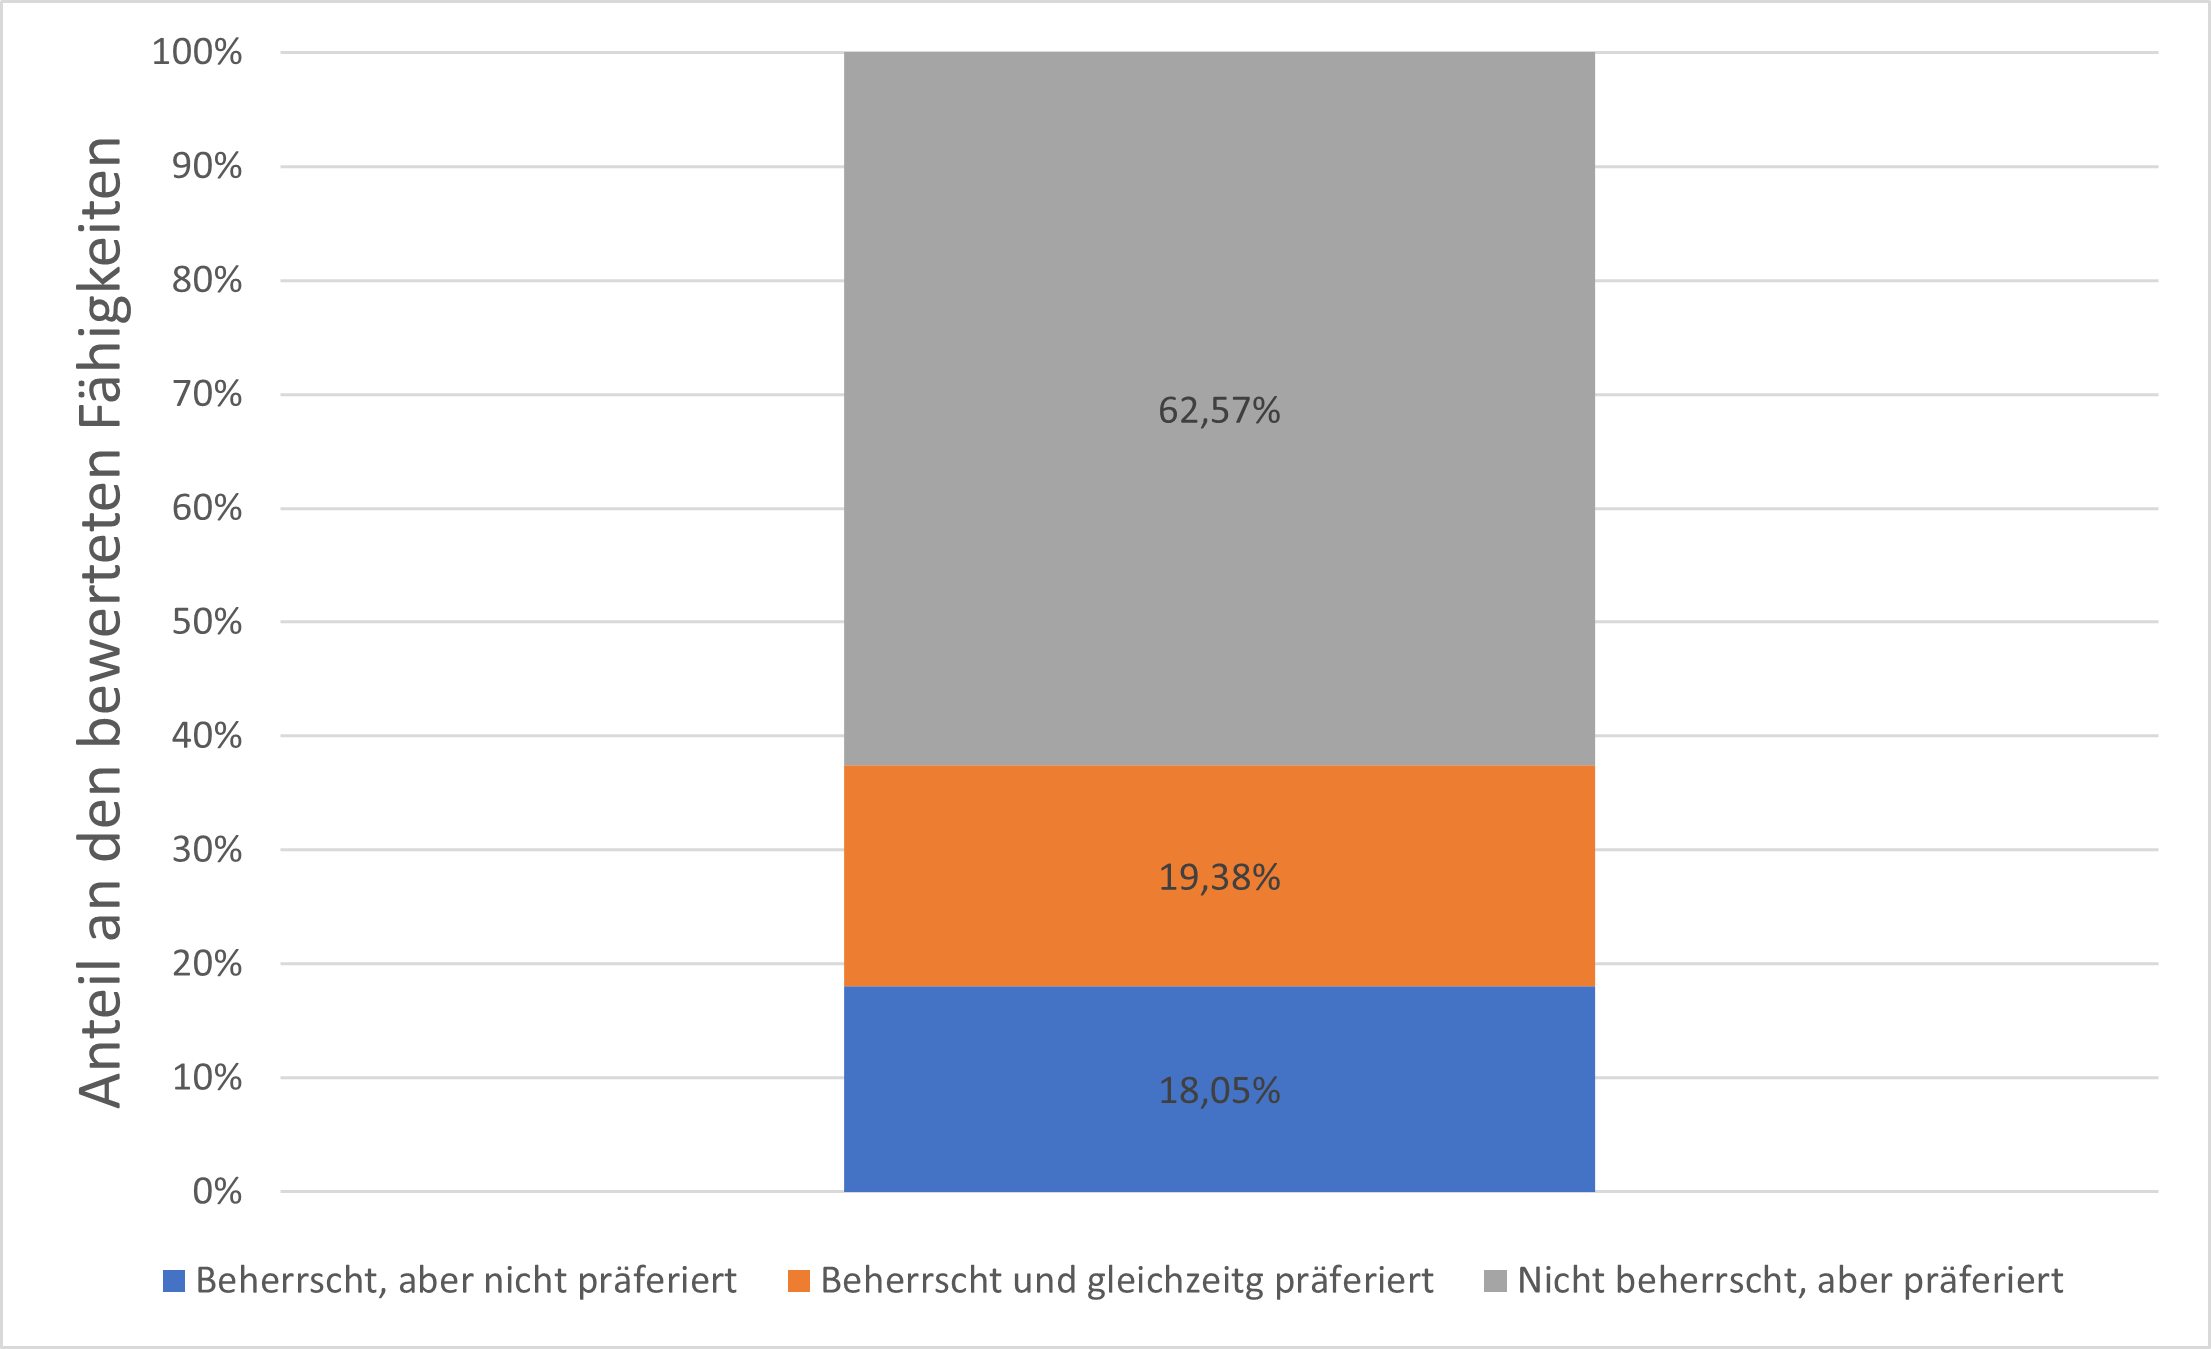
\includegraphics[width=1\textwidth]{gfx/auswertung-anteil-an-faehigkeiten.png}
	\caption{Anteil beherrschter und präferierter Fähigkeiten bei einem durchschnittlichen Mitarbeiter}
	\label{fig:ergebnisse:analyse:abb3}
\end{figure}

In Abbildung \ref{fig:ergebnisse:analyse:abb3} ist zu erkennen, dass ein durchschnittlicher Angestellter etwa 28 bzw. ca. 37.4 Prozent seiner insgesamt beurteilten Kompetenzen gleichzeitig beherrscht (orangene und blaue Farbe). Von diesen Fähigkeiten präferiert er jedoch nur ca. 14.5, also knapp über die Hälfte (orangene Farbe). Demgegenüber stehen ca. 46.7 bzw. etwa 62.6 Prozent an Fähigkeiten, welche der Angestellte zwar präferiert, aber noch nicht beherrscht (graue Farbe).

%Bei Betrachtung der beherrschten Fähigkeiten ist festzustellen, dass kaum Unterschiede zwischen präferierten und nicht gewünschten Kompetenzen ausgemacht werden können. So verfügt die durchschnittliche beherrschte, aber nicht gewünschte Fähigkeit (blaue Farbe in Abbildung \ref{fig:ergebnisse:analyse:abb3}) über eine Bewertung von 2.9 im Intranet. Die durchschnittliche vorhandene und gleichzeitig präferierte Kompetenz (orangene Farbe in Abbildung \ref{fig:ergebnisse:analyse:abb3}) verfügt über eine Bewertung von 3.1. Wie in Abbildung \ref{fig:ergebnisse:analyse:abb4} zu erkennen, sind auch bei Betrachtung der Fähigkeiten auf ihren jeweiligen Kompetenzniveaus kaum Differenzen auszumachen.
%\begin{figure}[h]
%	\centering
%	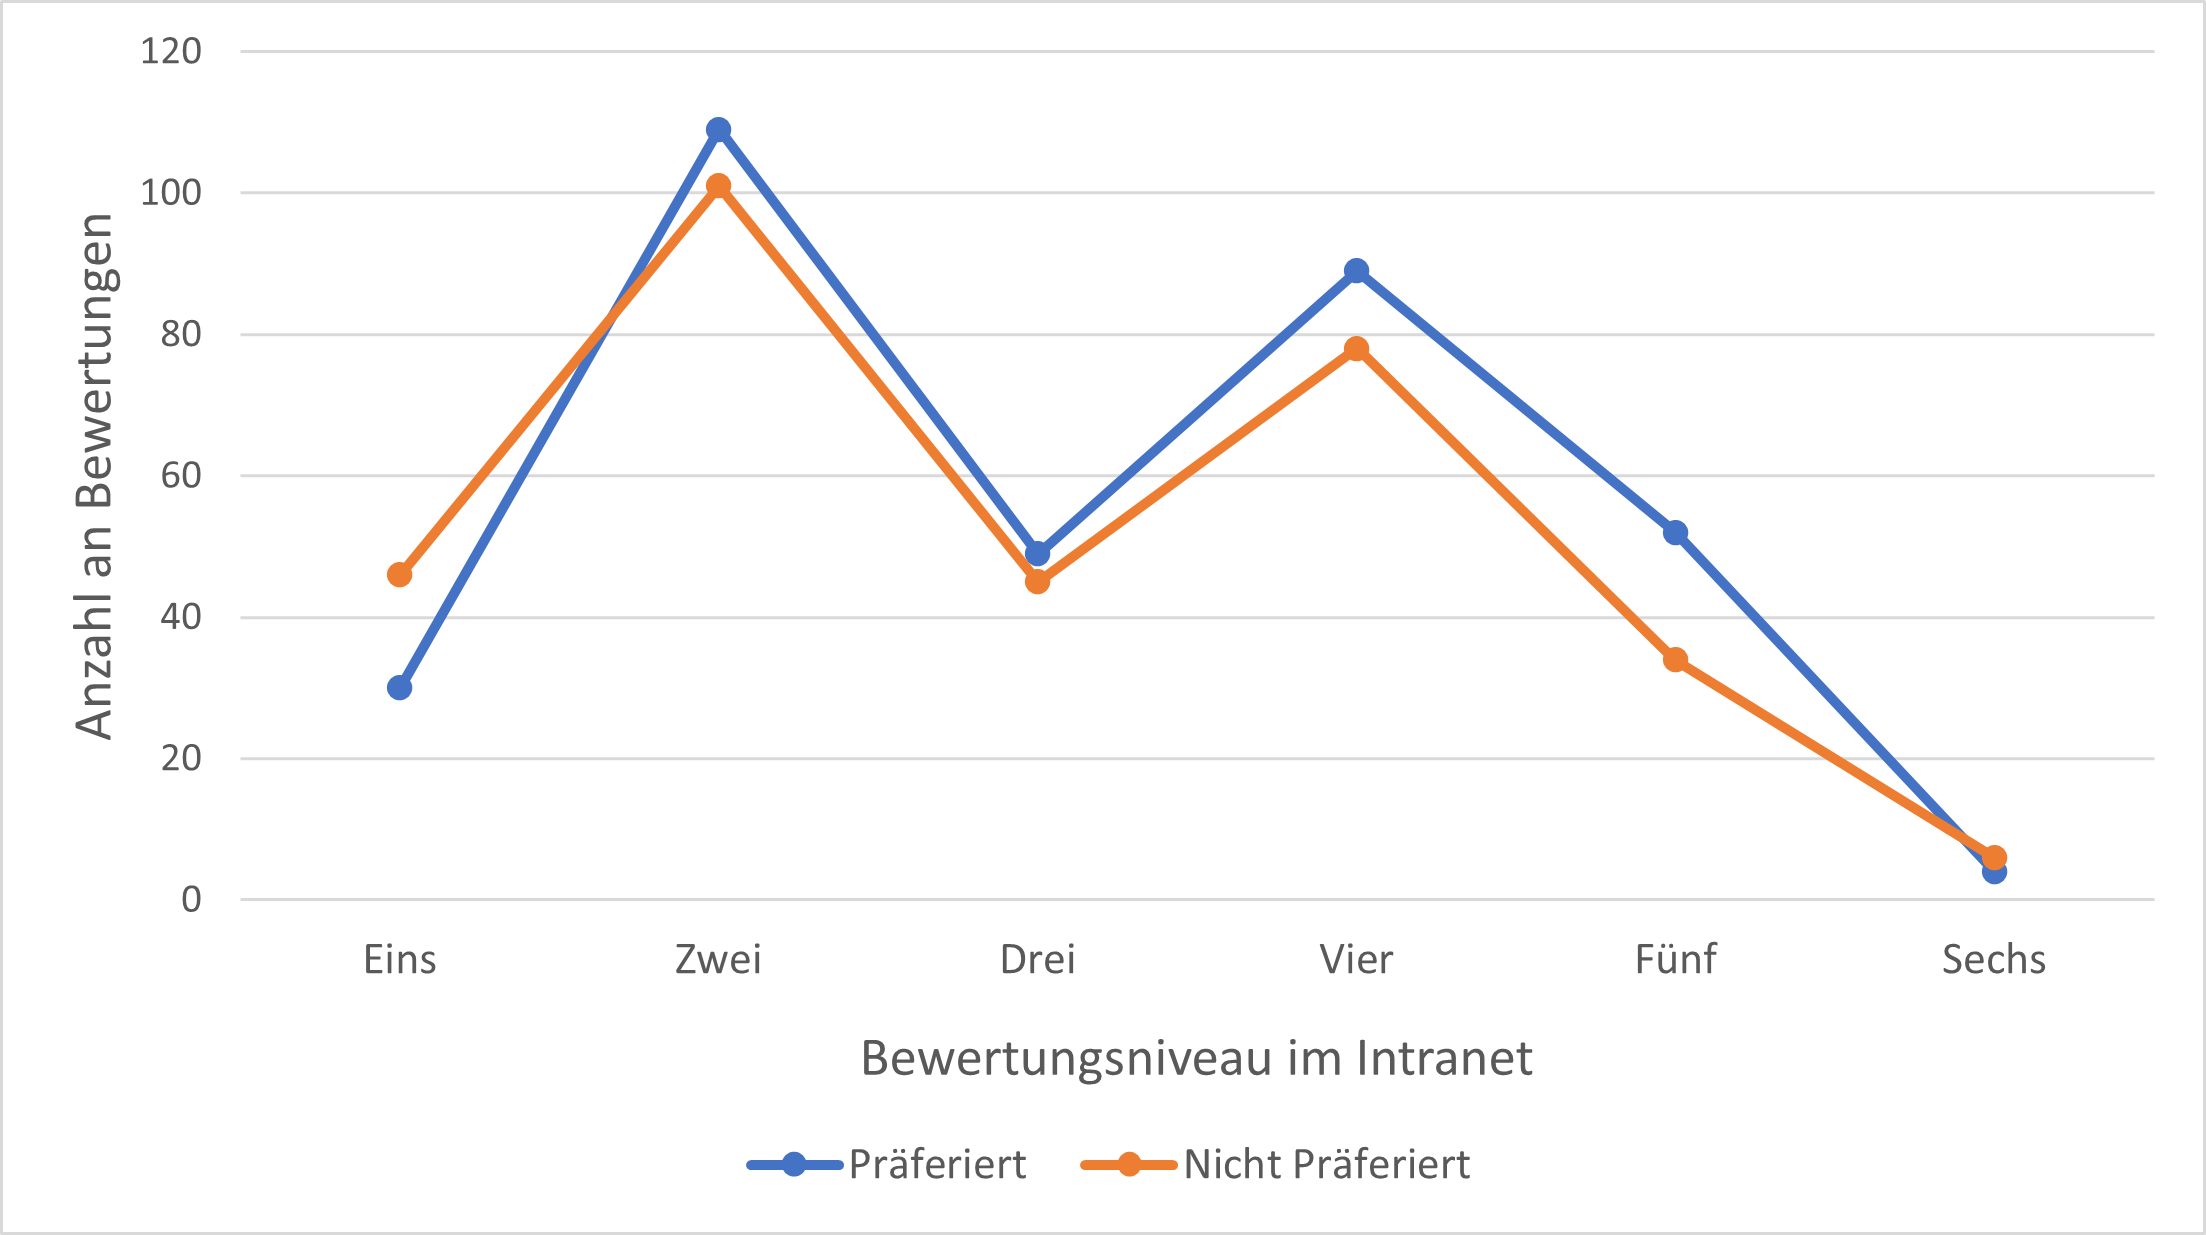
\includegraphics[width=0.8\textwidth]{gfx/bewertungen-je-bewertungsniveau.png}
%	\caption{Anzahl beherrschter und präferierter Fähigkeiten je Bewertungsniveau}
%	\label{fig:ergebnisse:analyse:abb4}
%\end{figure}
%Bei Analyse der präferierten Fähigkeiten (graue Farbe in Abbildung \ref{fig:ergebnisse:analyse:abb3}) ist zu beobachten, dass es sich bei den meist gewünschten Kompetenzen hauptsächlich um moderne Produkte aus dem Web- und Cloud-Umfeld handelt. So zählen neben Git und Java beispielsweise Kotlin, Kubernetes, Docker, Spring Boot und AWS zu den meist präferierten Fähigkeiten.

\subsection{Gesuchte und vorhandene Fähigkeiten und Präferenzen}
\label{ch:ergebnisse:umfrageMitarbeiter:projekte}
Zur Beantwortung der Forschungsfrage wurden im Rahmen der vorliegenden Master-Thesis fünf beispielhafte Projektpositionen definiert und in Kapitel \ref{ch:methodik:evaluation} vorgestellt. Abbildung \ref{fig:ergebnisse:analyse:abb5} zeigt für jede dieser Projektpositionen, wie viele der befragten Mitarbeiter im Durchschnitt die gesuchten Fähigkeiten beherrschen bzw. präferieren.

\begin{figure}[h]
	\centering
	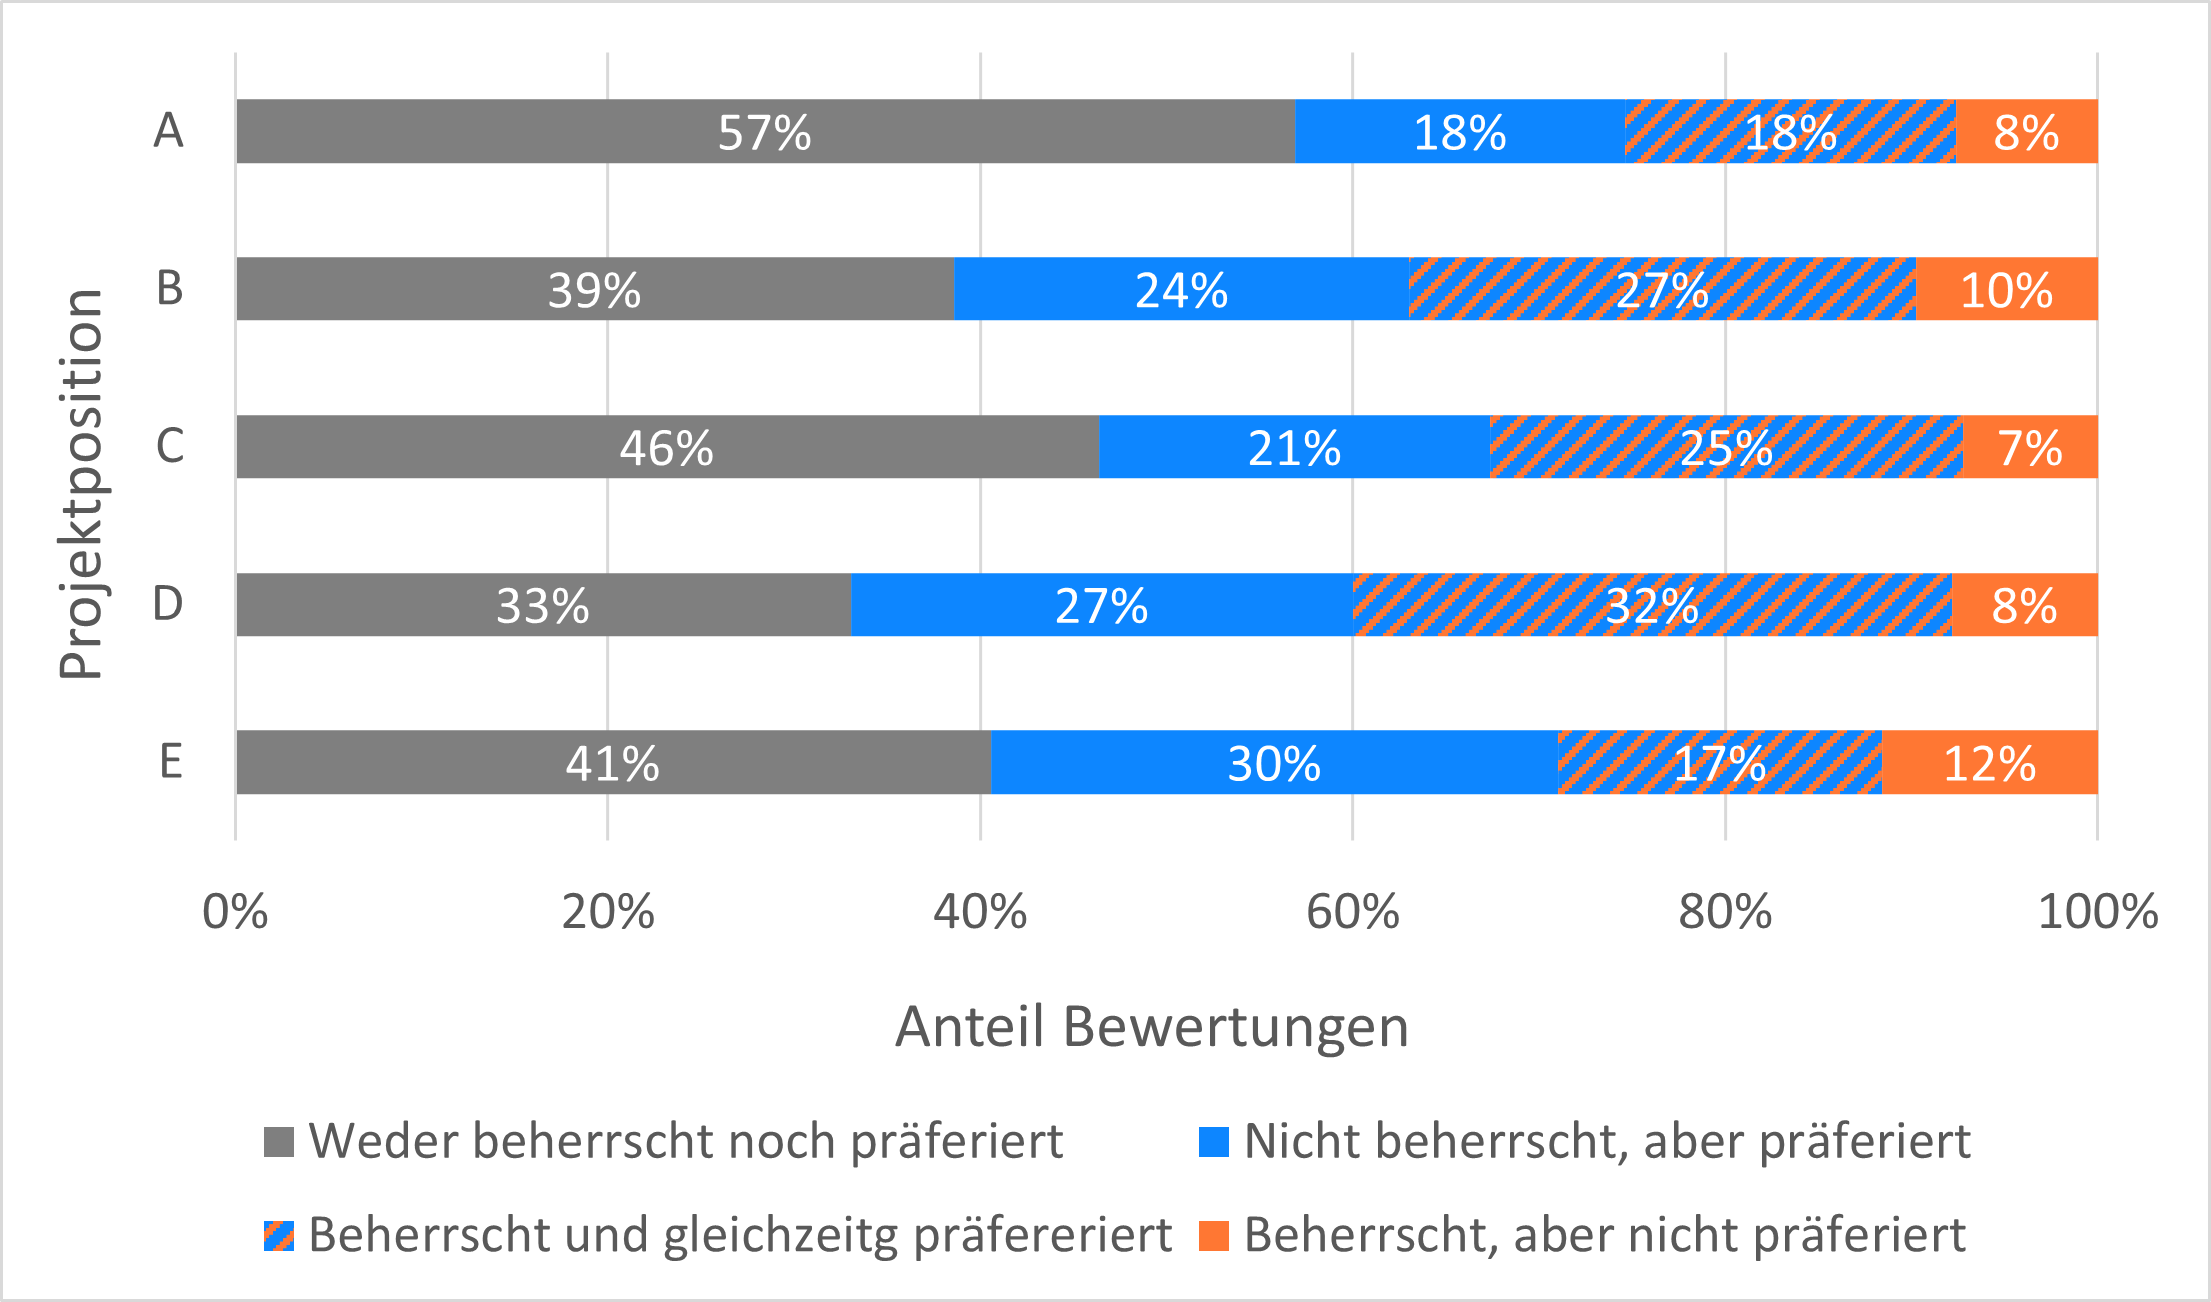
\includegraphics[width=1\textwidth]{gfx/anteil-bewertungen-je-projektposition.png}
	\caption{Anteil an Mitarbeitern, welche die in den Beispielprojektpositionen gesuchten Fähigkeiten im Durchschnitt beherrschen bzw. präferieren}
	\label{fig:ergebnisse:analyse:abb5}
\end{figure}

In Abbildung \ref{fig:ergebnisse:analyse:abb5} ist zu erkennen, dass durchschnittlich 33 Prozent aller Mitarbeiter bereits über die für die Projektpositionen benötigten Fähigkeiten verfügen. Dementsprechend beherrschen 67 Prozent aller Mitarbeiter die durchschnittlich gesuchte Kompetenz noch nicht. Es ist ebenfalls du beobachten, dass 60 Prozent aller Angestellten, welche die durchschnittlich gesuchte Kompetenz beherrschen, diese gleichzeitig präferieren. Auch ist zu erkennen, dass die Anteile an Mitarbeitern, welche die durchschnittlich gesuchte Fähigkeit beherrschen und gleichzeitig präferieren und Angestellten, welche die im Durchschnitt benötigte Kompetenz noch nicht beherrschen und dennoch präferieren mit je 24 Prozent gleich groß sind.

Bei Betrachtung jeder einzelnen in den Beispielprojektpositionen gesuchten Fähigkeit ergibt sich die Darstellung aus Abbildung \ref{fig:ergebnisse:analyse:abb6}.

\begin{figure}[h]
	\centering
	
	\subfloat[Projektposition A]{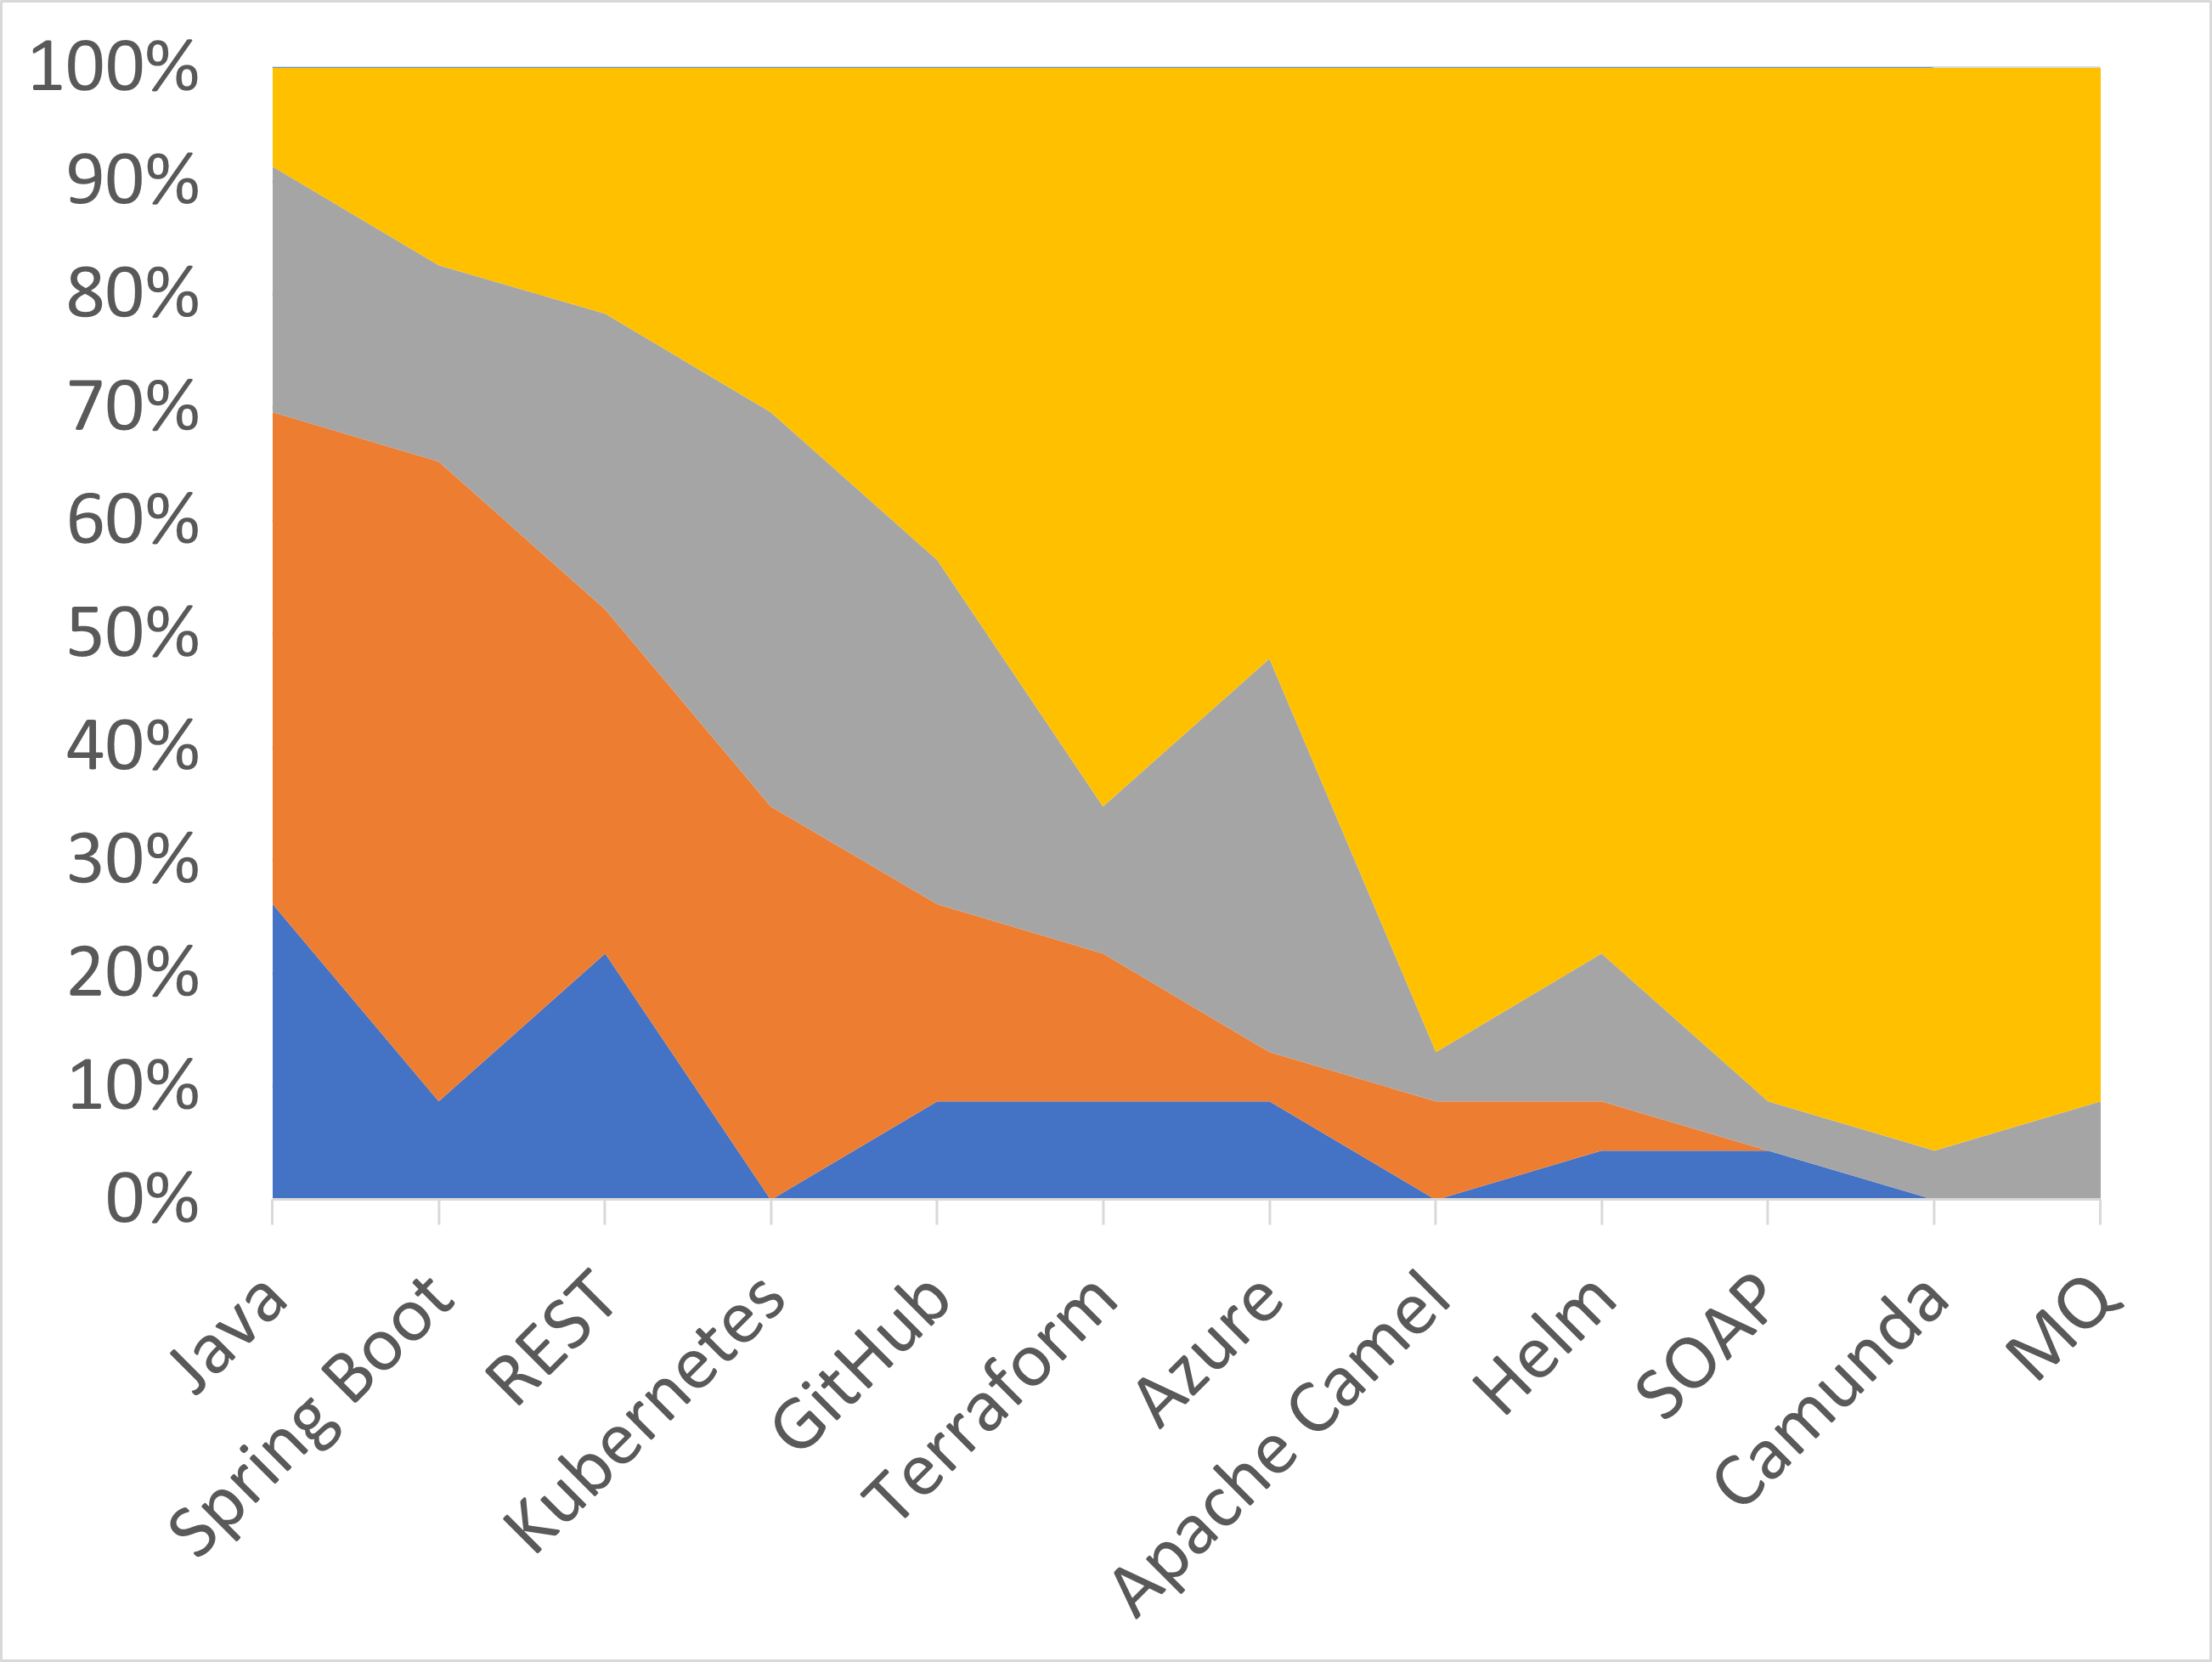
\includegraphics[width = 0.4\textwidth]{gfx/projekt-detail-a.png}}
	\subfloat[Projektposition B]{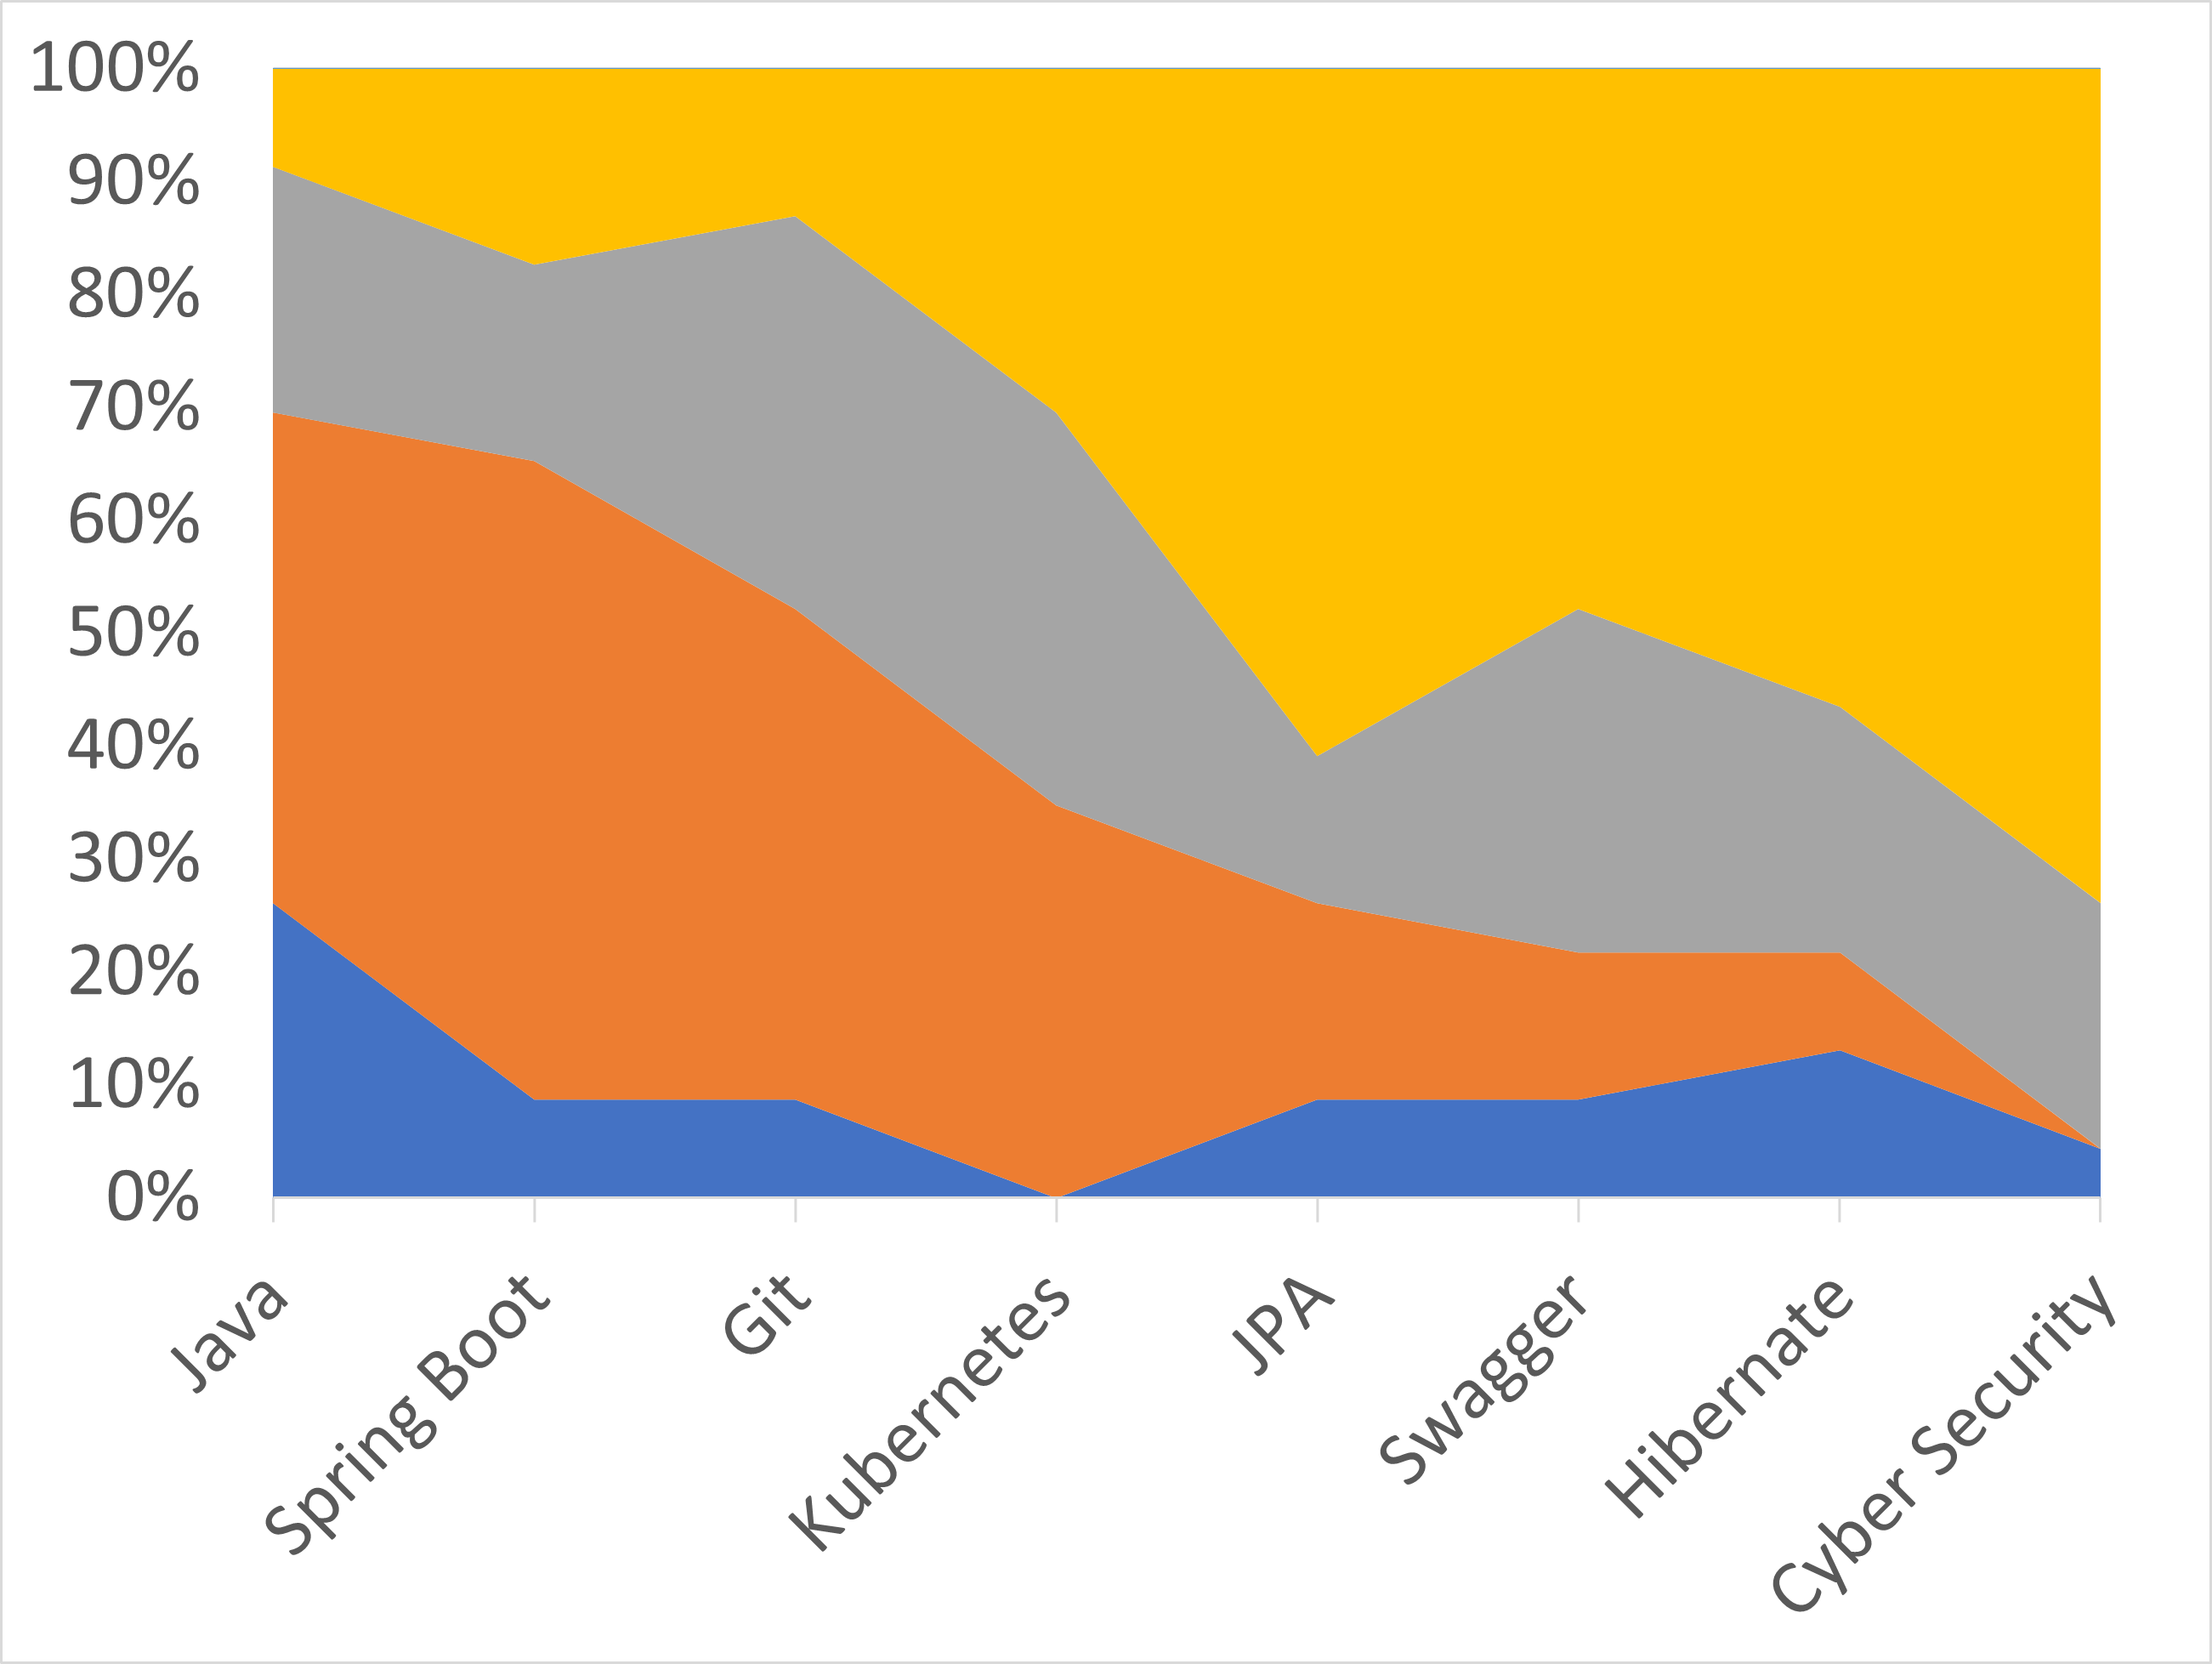
\includegraphics[width = 0.4\textwidth]{gfx/projekt-detail-b.png}}
	
\end{figure}
\begin{figure}[h]
	\centering
	\ContinuedFloat
	
	\subfloat[Projektposition C]{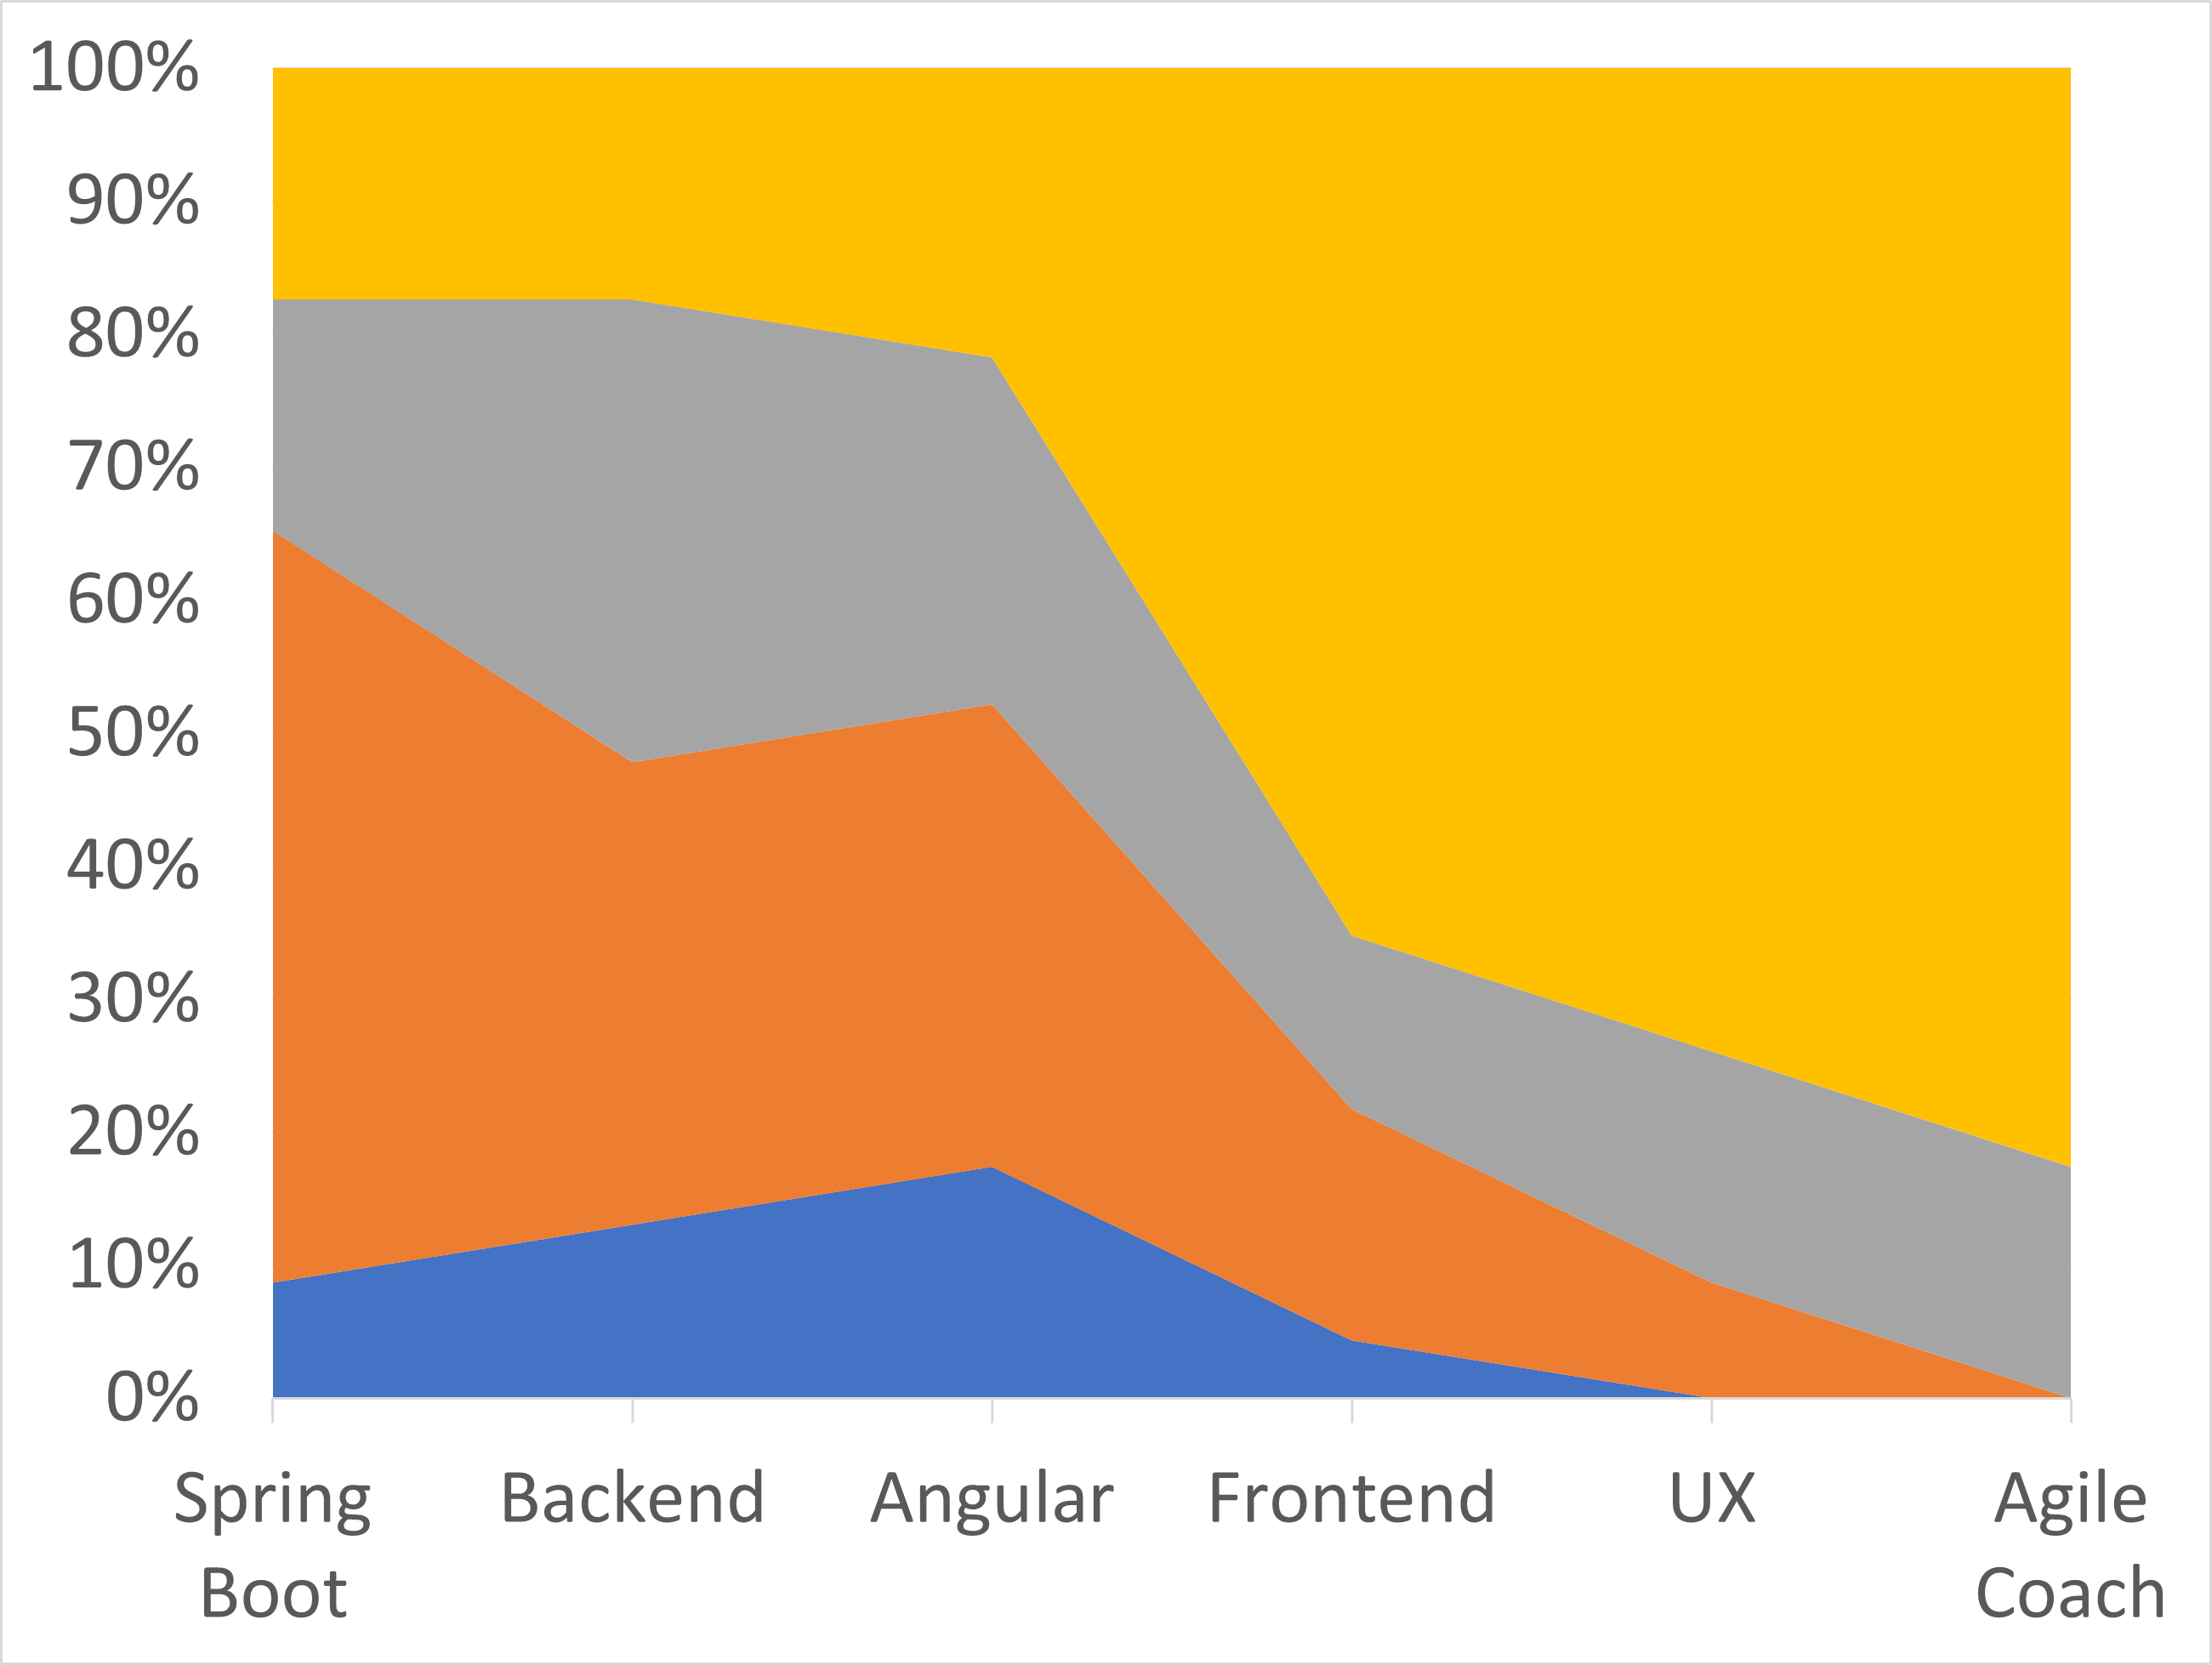
\includegraphics[width = 0.4\textwidth]{gfx/projekt-detail-c.png}}
	\subfloat[Projektposition D]{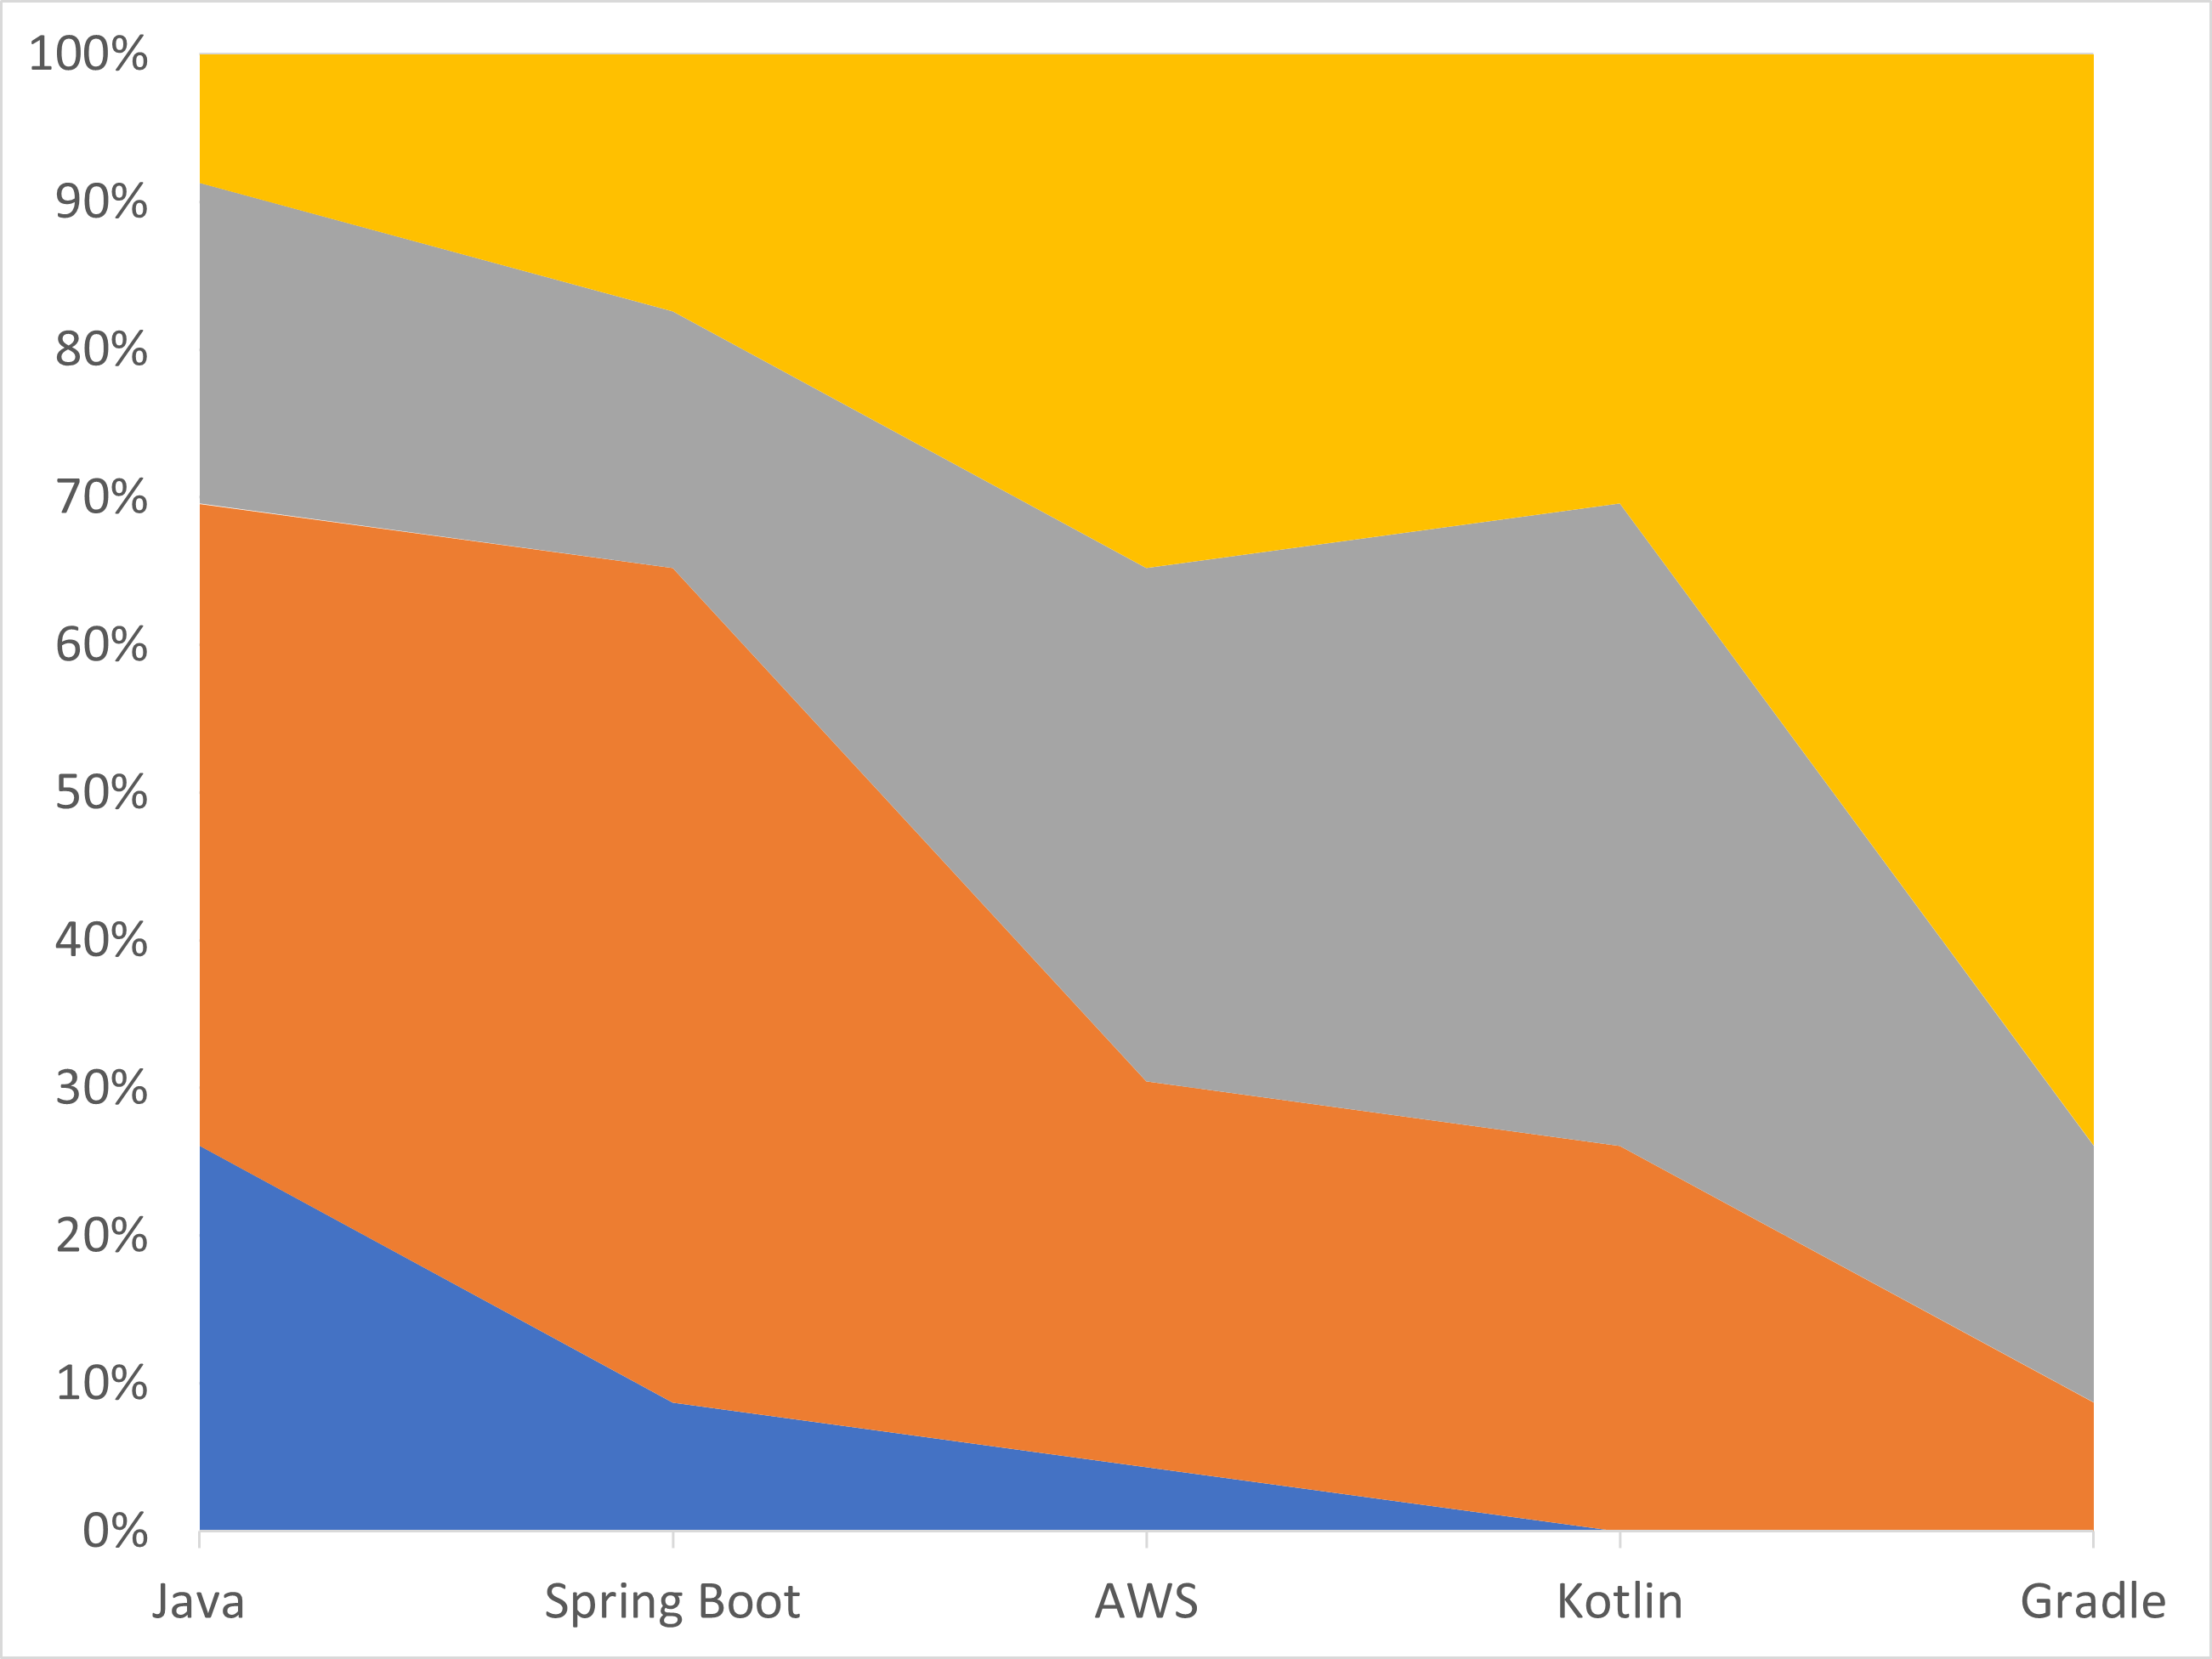
\includegraphics[width = 0.4\textwidth]{gfx/projekt-detail-d.png}}
	
\end{figure}
\begin{figure}[h]
	\centering
	\ContinuedFloat
	
	\subfloat[Projektposition E]{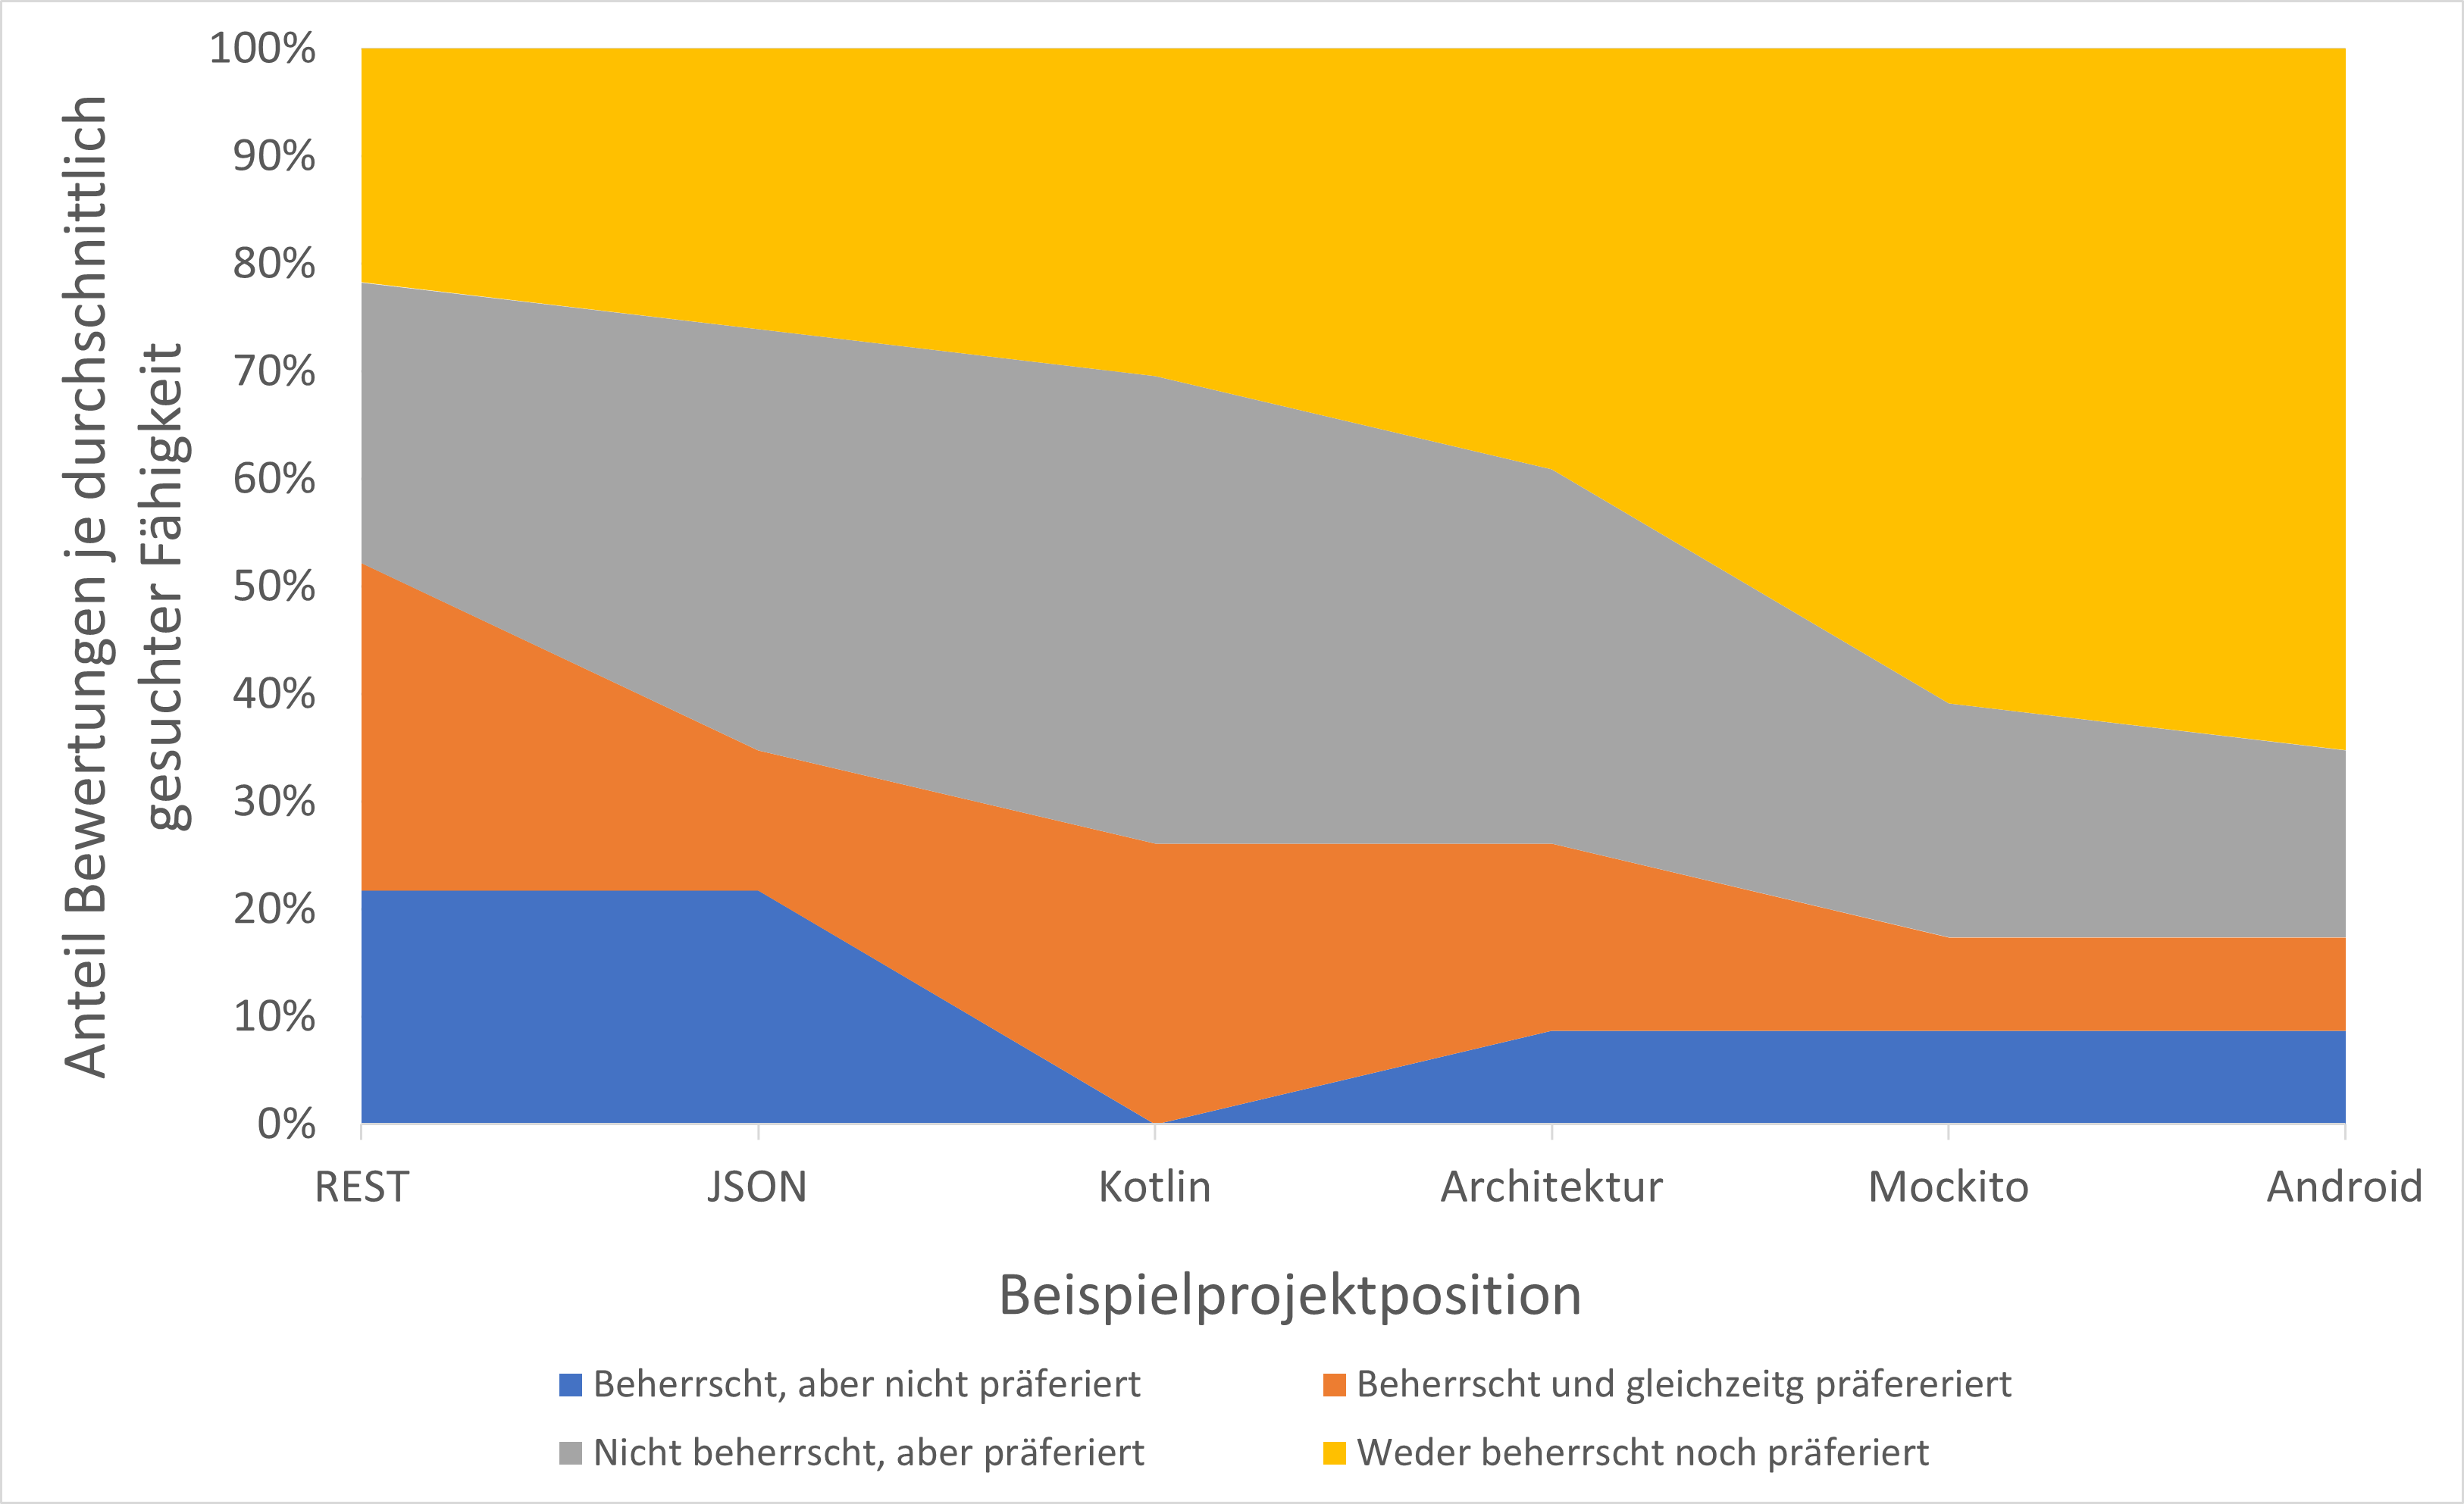
\includegraphics[width = 0.4\textwidth]{gfx/projekt-detail-e.png}}
	\subfloat[Legende]{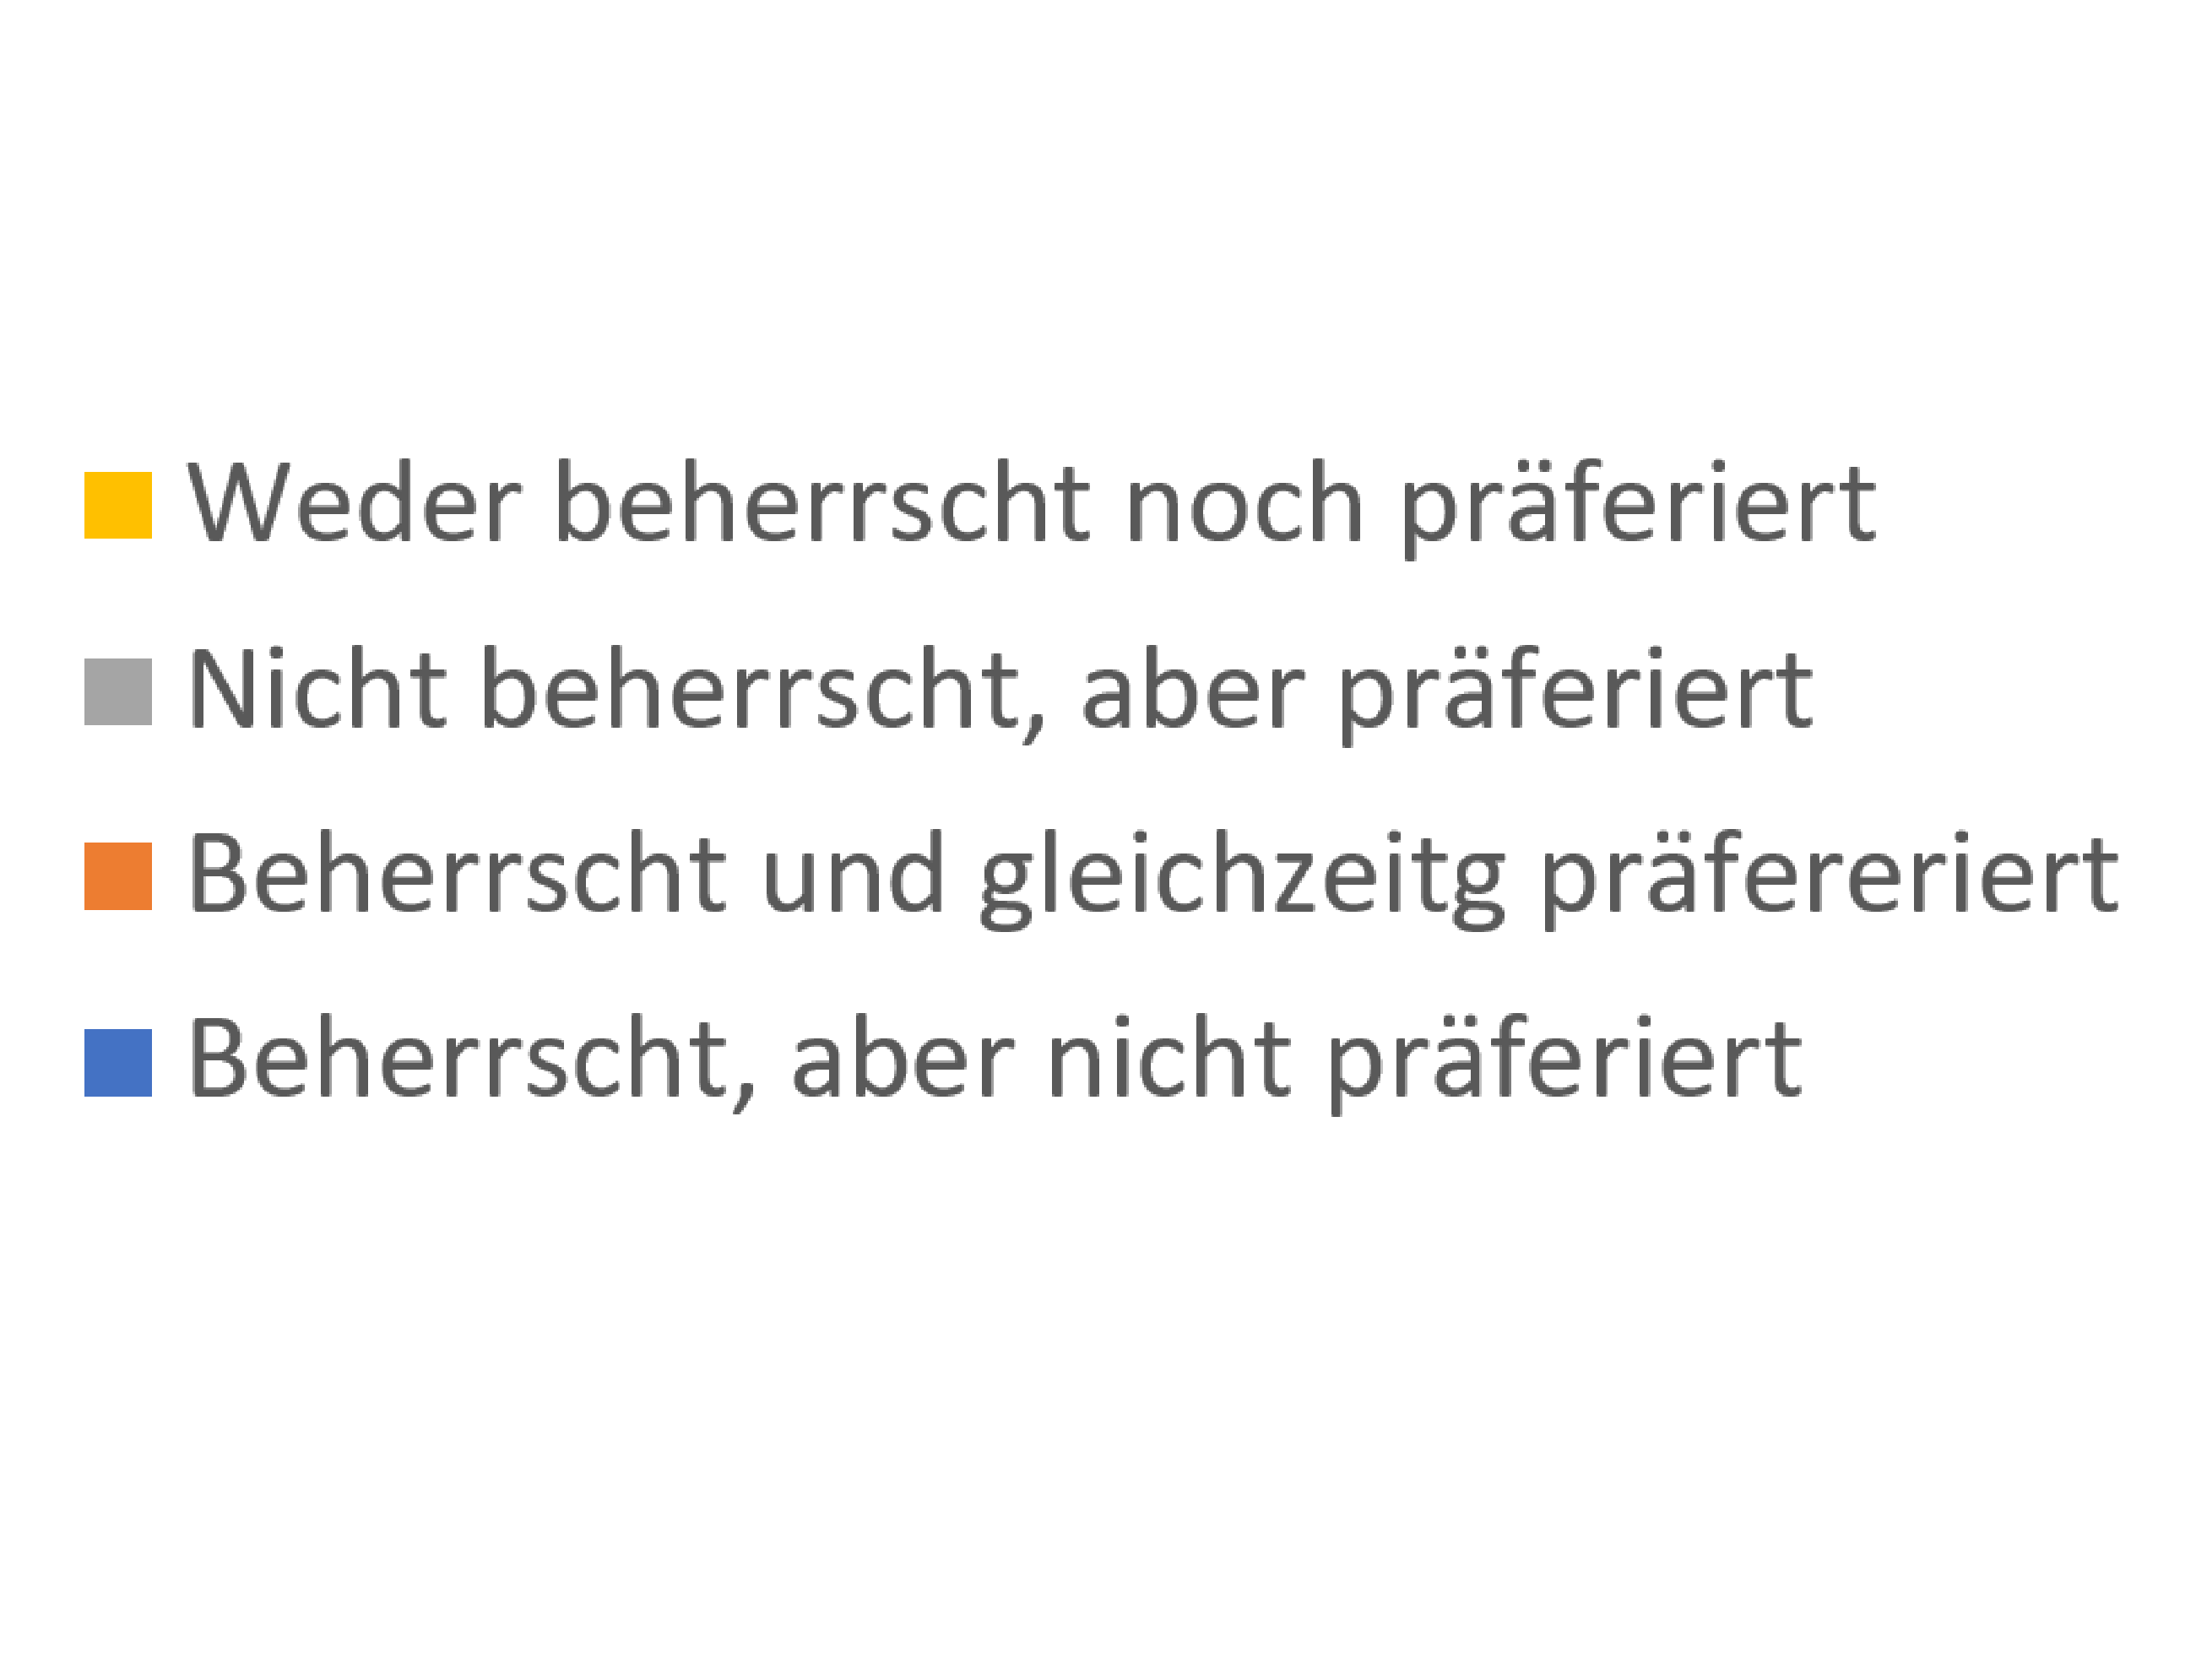
\includegraphics[width = 0.4\textwidth]{gfx/projekt-detail-legende.png}}
	
	\caption{Anteil an Mitarbeitern, welche die in den jeweiligen Beispielprojektpositionen gesuchten Fähigkeiten beherrschen bzw. präferieren}
\label{fig:ergebnisse:analyse:abb6}
\end{figure}

In Abbildung \ref{fig:ergebnisse:analyse:abb6} ist zu erkennen, dass im Durchschnitt 31 Prozent der gesuchten Fähigkeiten jedes Projekts von mindestens der Hälfte aller Mitarbeiter beherrscht werden. Für die übrigen 69 Prozent der Kompetenzen ist anschließend ein zumeist lineares Absinken der Angestellten zu beobachten, welche über diese Fähigkeiten verfügen. Wie stark die Abnahme ist, unterscheidet sich zwischen den einzelnen Projektpositionen stark. So beherrschen bei Projektposition E 17 Prozent aller Mitarbeiter mindestens eine Fähigkeit. Bei den Projektpositionen A und C werden dagegen 17 Prozent der gesuchten Fähigkeiten von keinem einzigen Angestellten beherrscht. In den Grafiken aus Abbildung \ref{fig:ergebnisse:analyse:abb6} ist außerdem zu beobachten, dass keine Kompetenz gesucht wird, welche kein einziger Angestellter in der Umfrage als Präferenz angegebene hat.

\section{Ergebnisse der Fallstudie}
\label{ch:ergebnisse:fallstudie}

\subsection{Erwartete Zufriedenheit der Projektmitarbeiter}
\label{ch:ergebnisse:fallstudie:umfrageMitarbeiter}
In der in Kapitel \ref{ch:methodik:evaluation} vorgestellten Umfrage wurde erhoben, welche Zufriedenheit die Mitarbeiter der EXXETA AG mit Tätigkeiten auf den Projektpositionen aus Abbildung \ref{fig:methodik:evaluation:abb2} prognostizieren. Die Ergebnisse sind in Tabelle \ref{tbl:ergebnisse:umfrageMitarbeiter:zufriedenheit:tbl1} dargestellt.%Dort sind unter "zufrieden" die Antwortmöglichkeiten "voll und ganz zufrieden" und "eher zufrieden" und unter "unzufrieden" die Optionen "weniger zufrieden" und "gar nicht zufrieden" zusammengefasst.

\begin{table}[h]
	\centering
	\begin{tabularx}{\textwidth}{X|X|X|X|X}
		\textbf{Projekt-position} & \textbf{Gar nicht zufrieden} & \textbf{Weniger zufrieden} & \textbf{Eher zufrieden} & \textbf{Voll und ganz zufrieden}\\ 
		\hline
		A & 4  & 4  & 10 & 5\\
		B & 3  & 6  & 7  & 7\\
		C & 10 & 7  & 4  & 2\\
		D & 5  & 7  & 7  & 4\\
		E & 5  & 10 & 4  & 4
	\end{tabularx}
	\caption{Anzahl an Mitarbeitern, welche zufrieden bzw. unzufrieden mit der Tätigkeit auf den jeweiligen Beispielprojektpositionen wären}
	\label{tbl:ergebnisse:umfrageMitarbeiter:zufriedenheit:tbl1}
\end{table}

In Tabelle \ref{tbl:ergebnisse:umfrageMitarbeiter:zufriedenheit:tbl1} ist zu erkennen, dass die Mitarbeiter überwiegend eine hohe Zufriedenheit mit den Projektpositionen A und B prognostizieren. Mit einer Tätigkeit auf den Projektpositionen C und E zeigen sich die Angestellten eher unzufrieden. Projektposition D stehen die Mitarbeiter gespalten gegenüber, sodass etwa die Hälfte der Befragten zufrieden und die andere Hälfte unzufrieden mit dieser Tätigkeit wäre.

Abbildung \ref{fig:ergebnisse:analyse:abb7} zeigt, für wie viele der 23 befragten Mitarbeiter der bilaterale Empfehlungsansatz gegenüber dem unilateralen Vorgehen für eine höhere Zufriedenheit seitens der Mitarbeiter sorgte. Wie in Kapitel \ref{ch:methodik:evaluation} beschrieben, entsteht eine höhere Zufriedenheit mit den Projekttätigkeiten, wenn das bilaterale System die Angestellten bei einer prognostizierten Zufriedenheit höher und bei einer erwarteten Unzufriedenheit niedriger positioniert als die unilaterale Anwendung.

\begin{figure}[h]
	\centering
	
	\subfloat[Projektposition A]{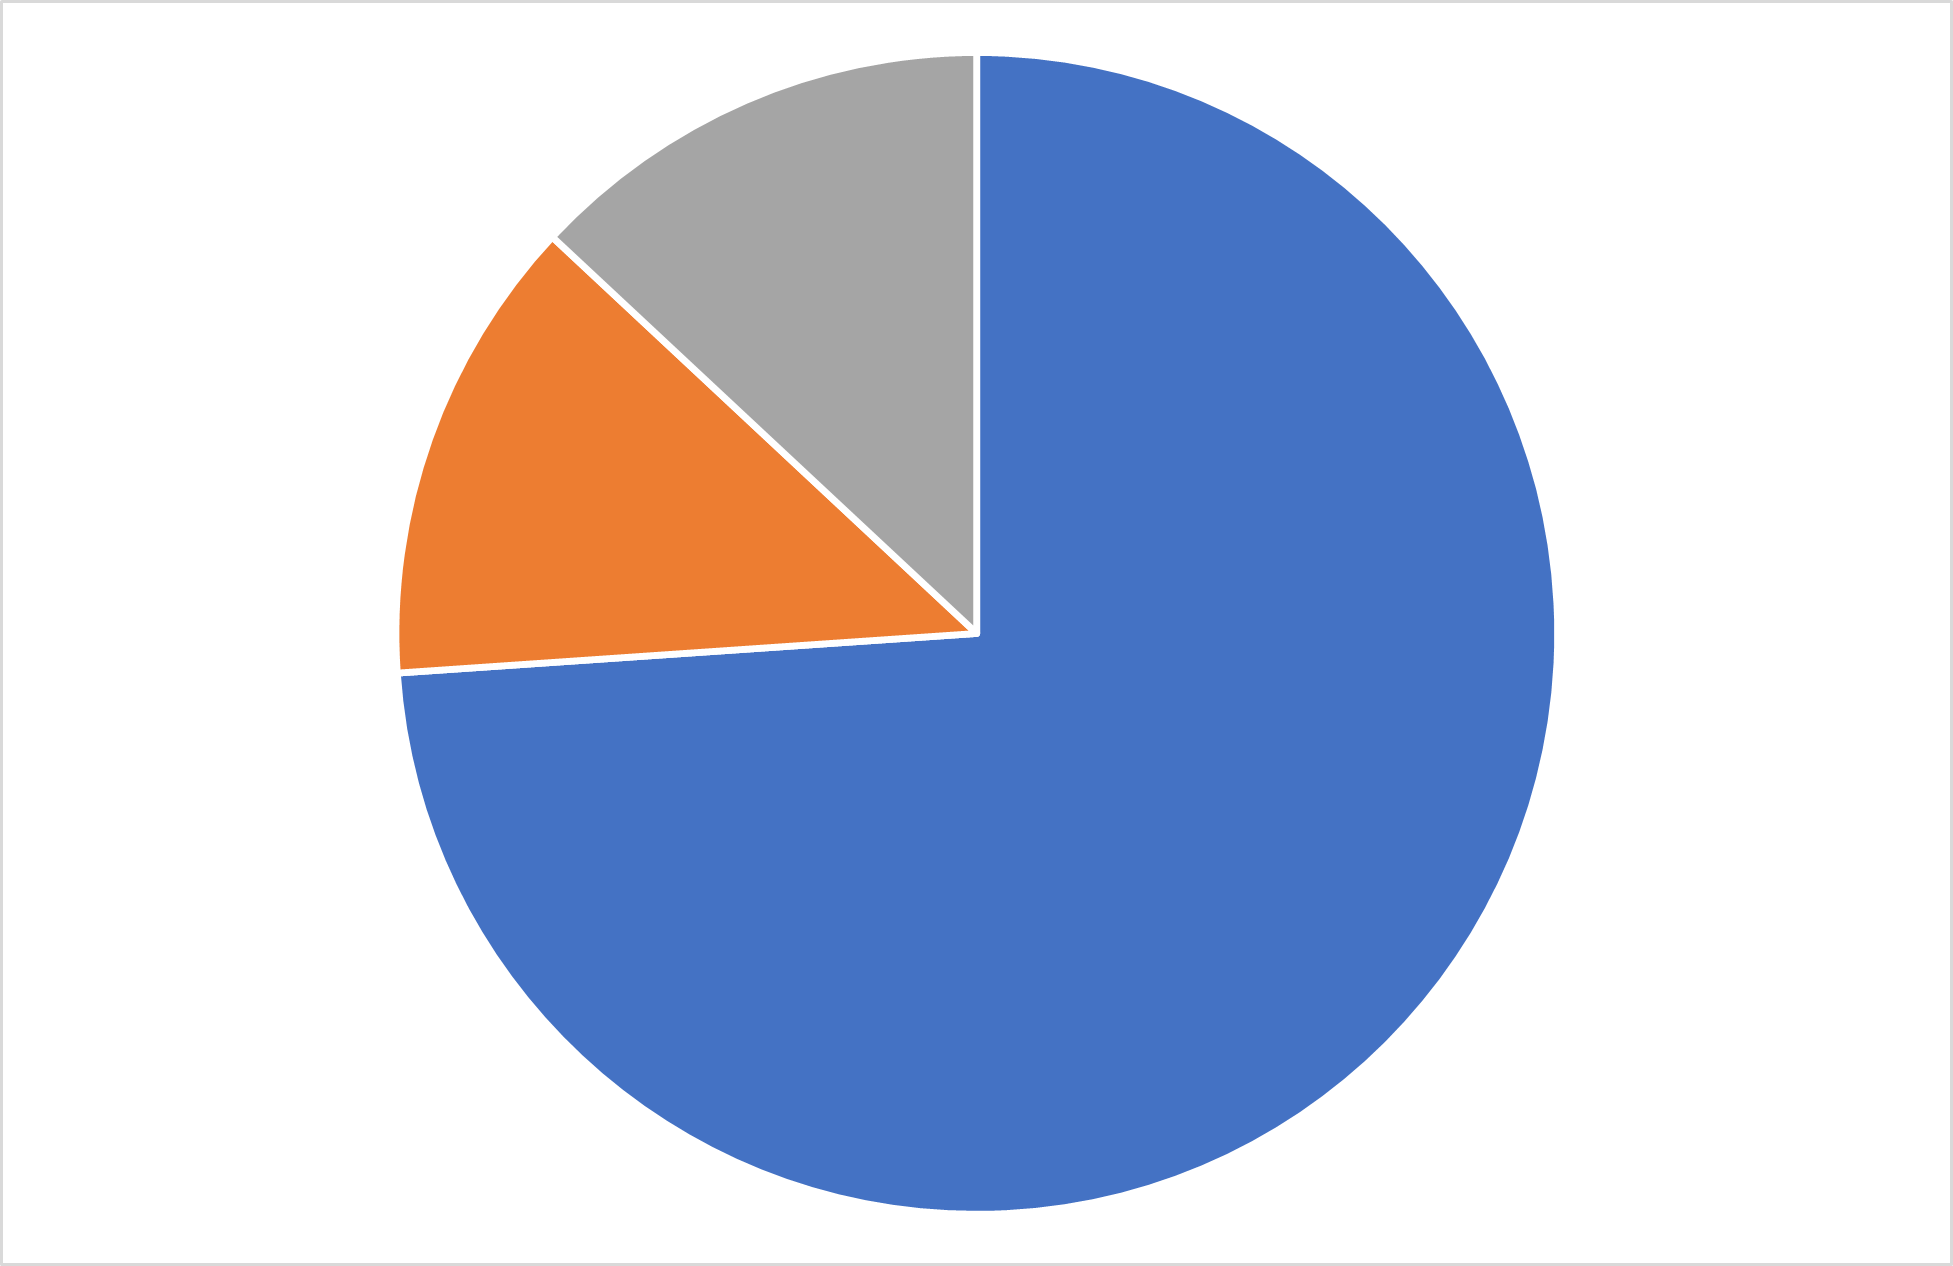
\includegraphics[width = 0.4\textwidth]{gfx/zufriedenheit-projekt-a.png}}
	\subfloat[Projektposition B]{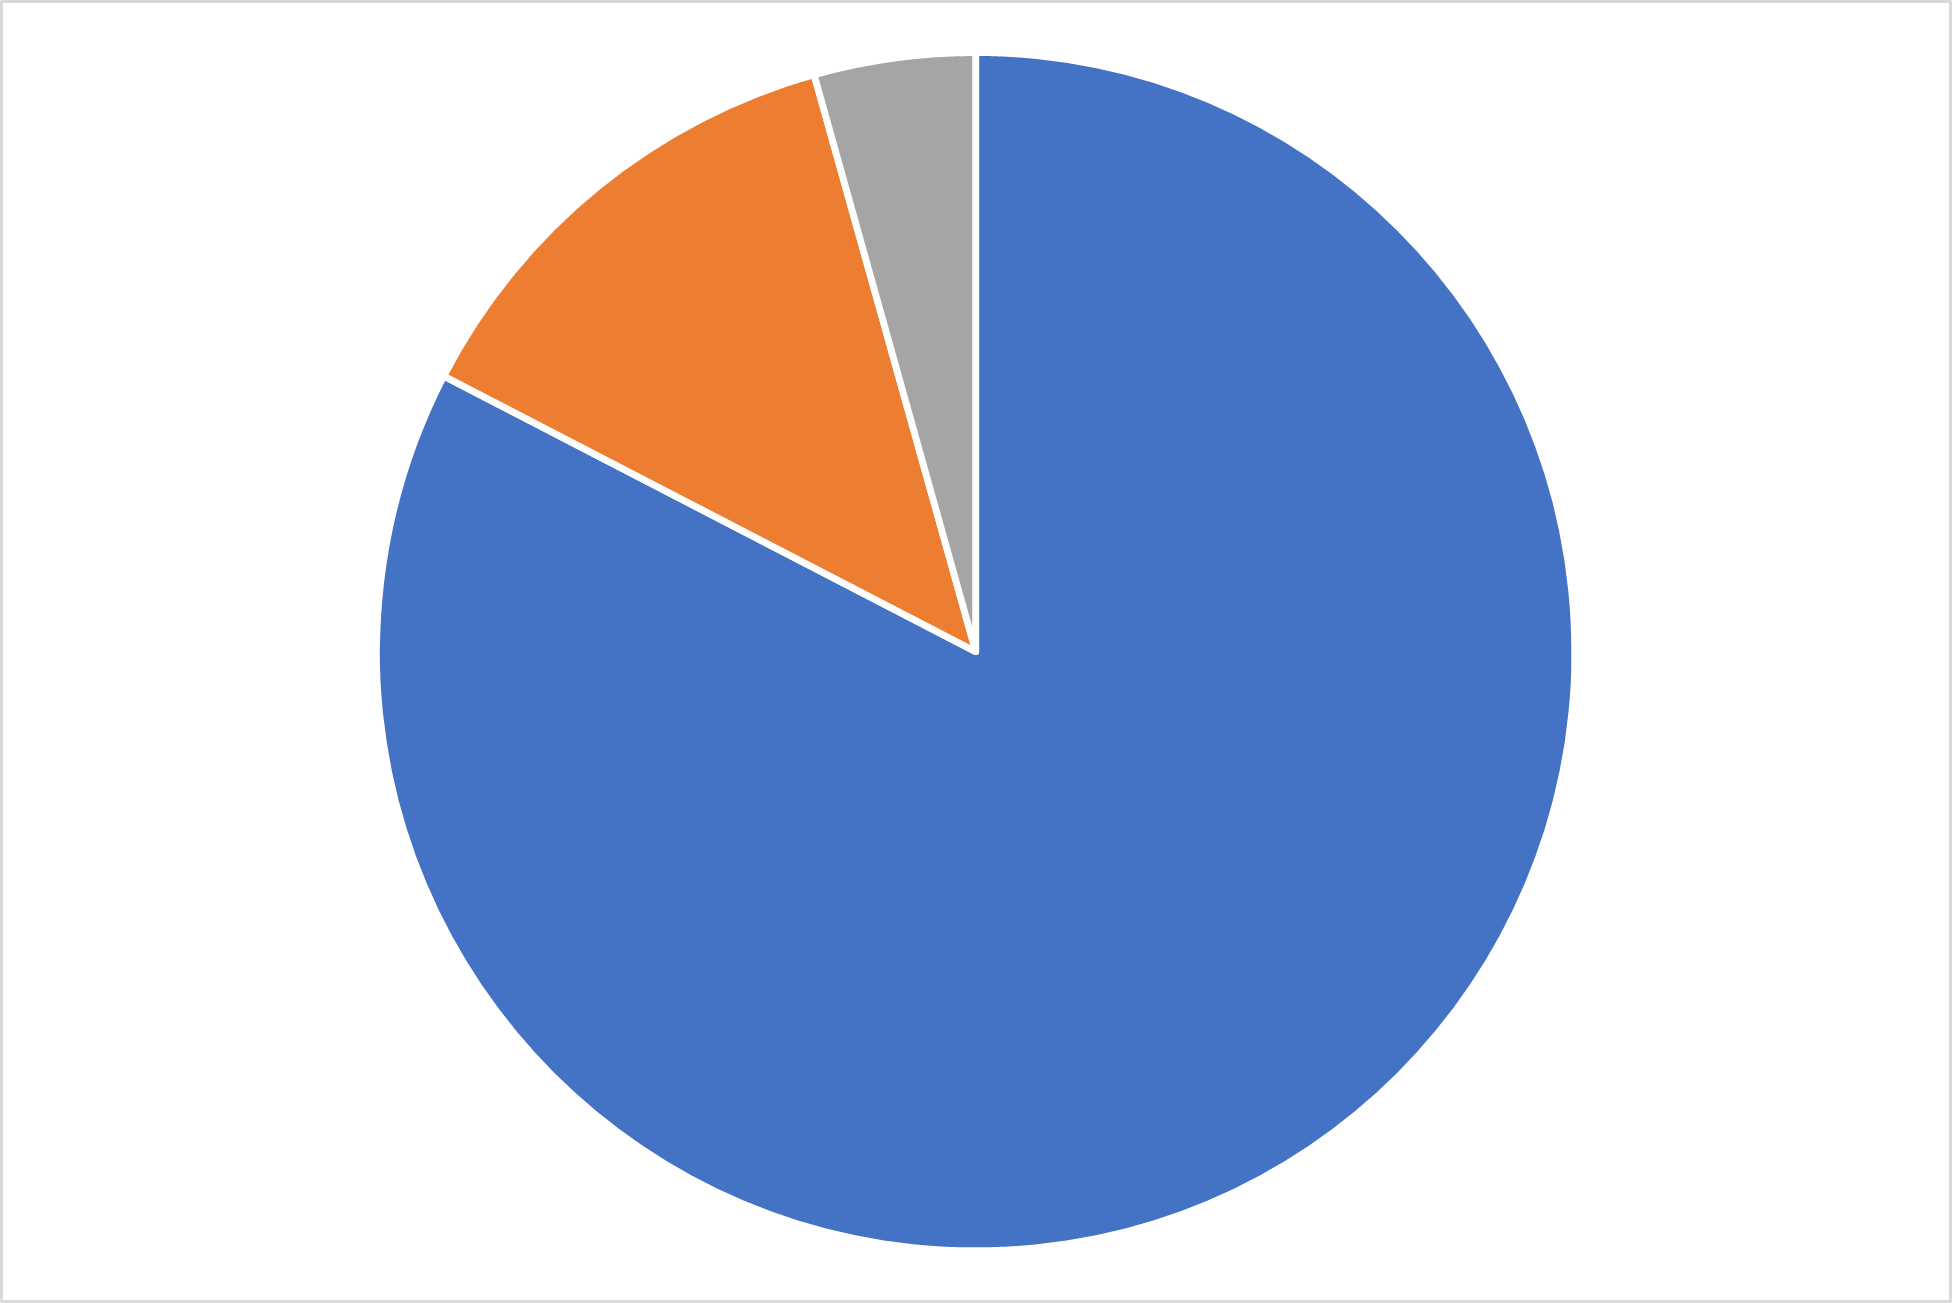
\includegraphics[width = 0.4\textwidth]{gfx/zufriedenheit-projekt-b.png}}
	\newline
	\subfloat[Projektposition C]{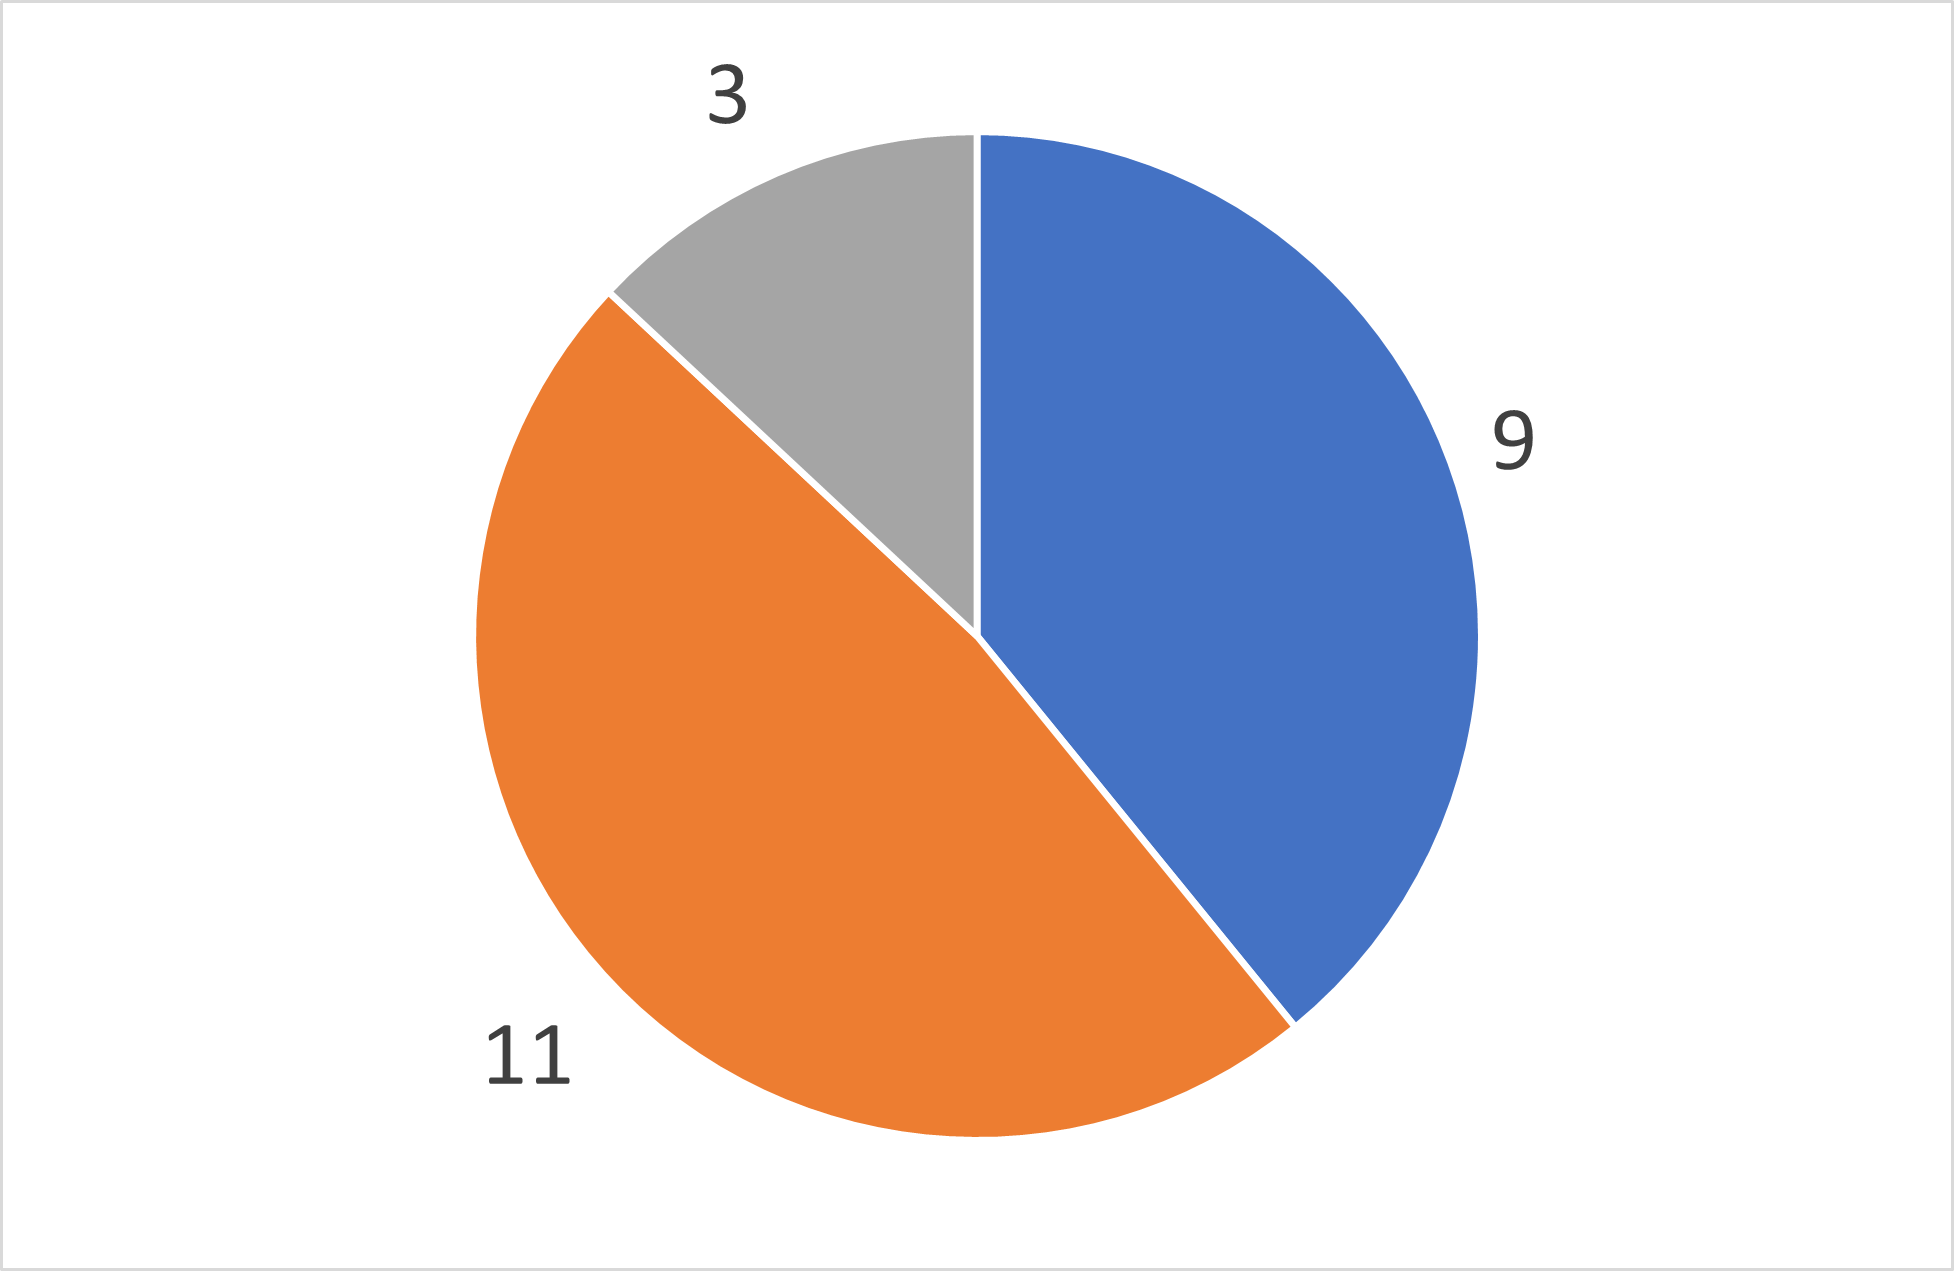
\includegraphics[width = 0.4\textwidth]{gfx/zufriedenheit-projekt-c.png}}
	\subfloat[Projektposition D]{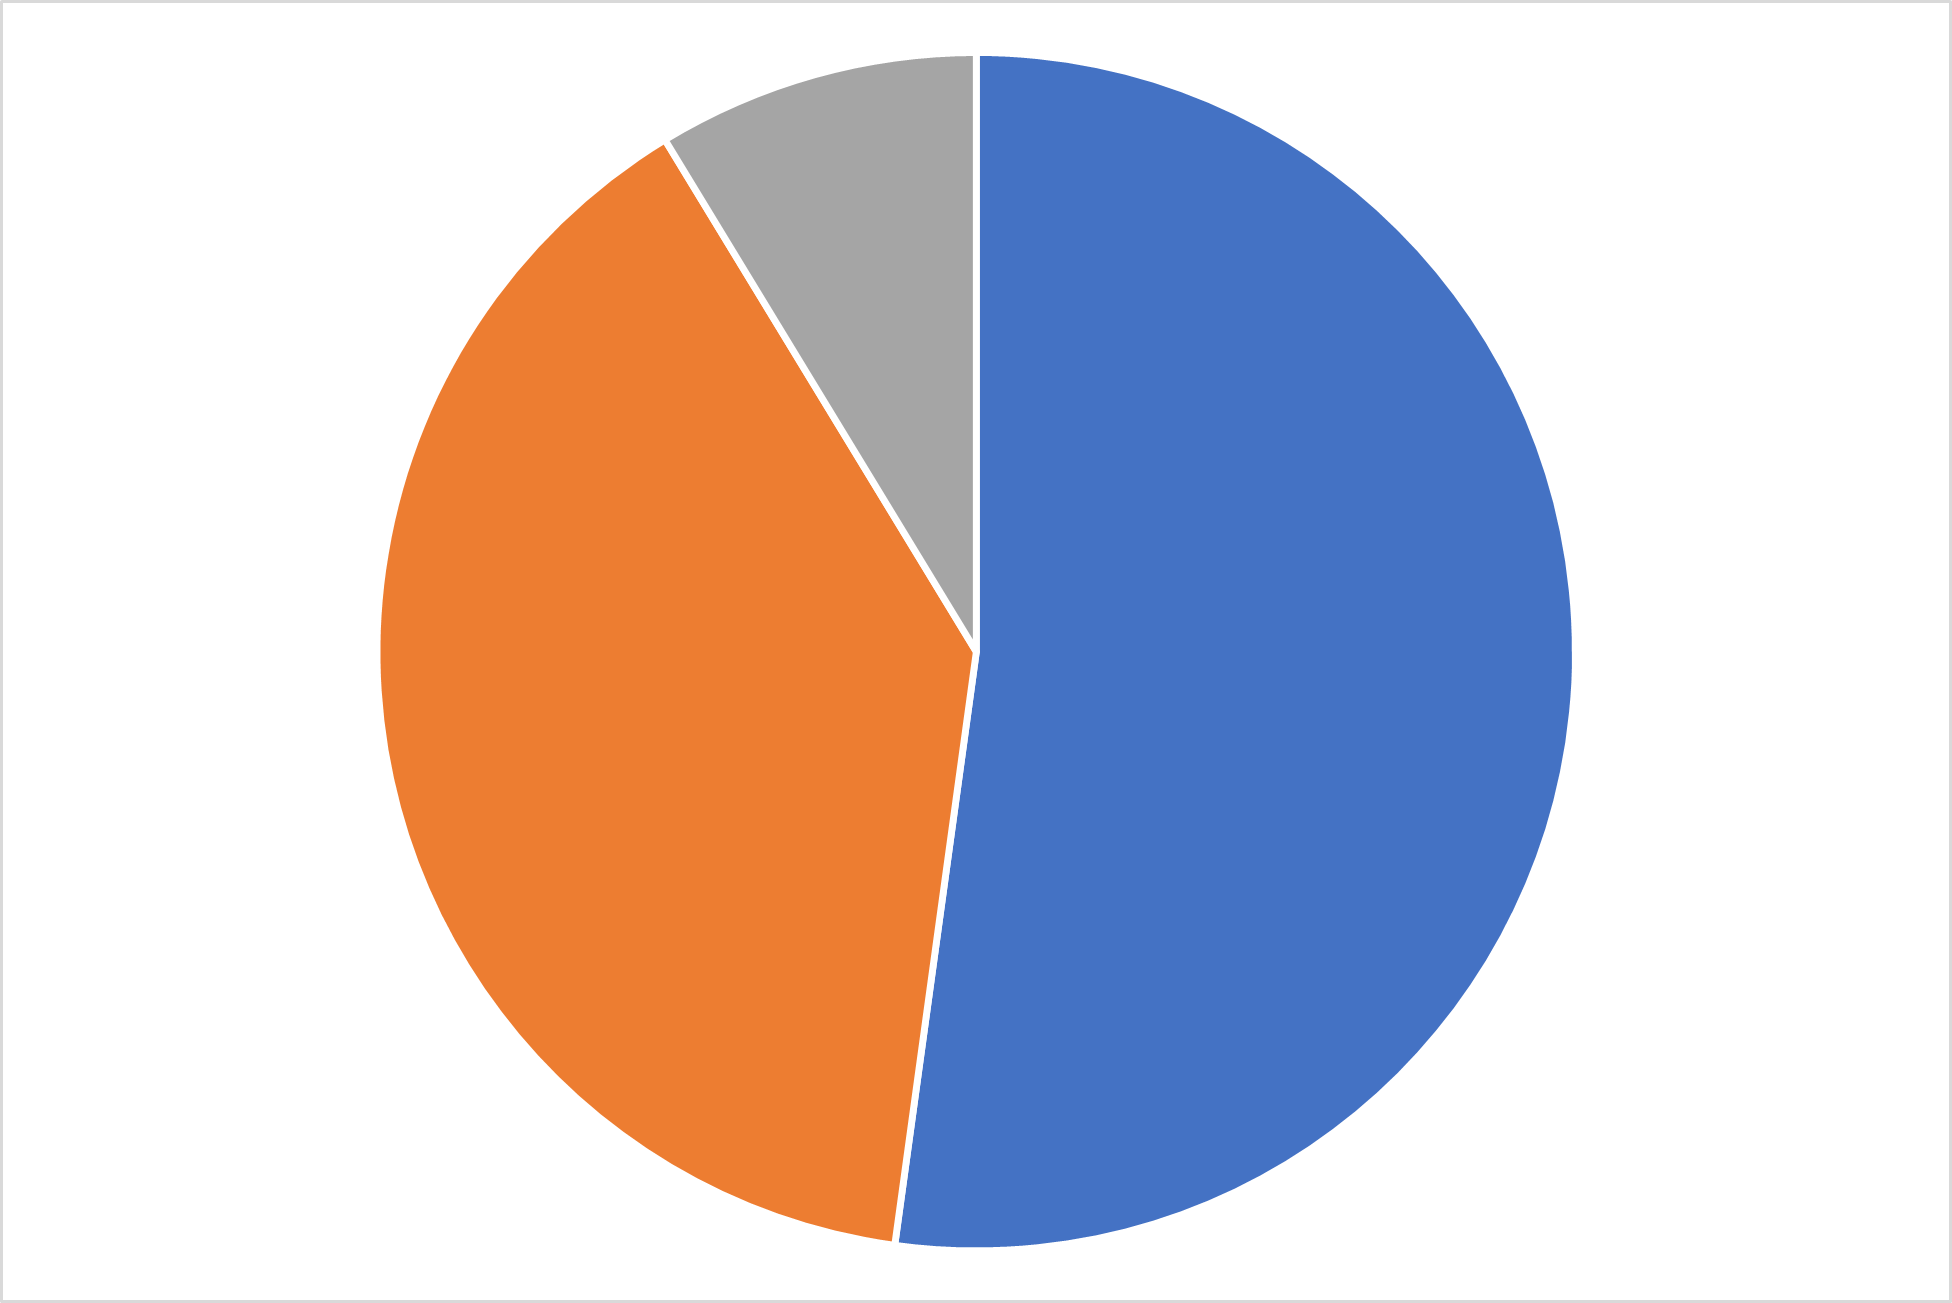
\includegraphics[width = 0.4\textwidth]{gfx/zufriedenheit-projekt-d.png}}
	\newline
	\subfloat[Projektposition E]{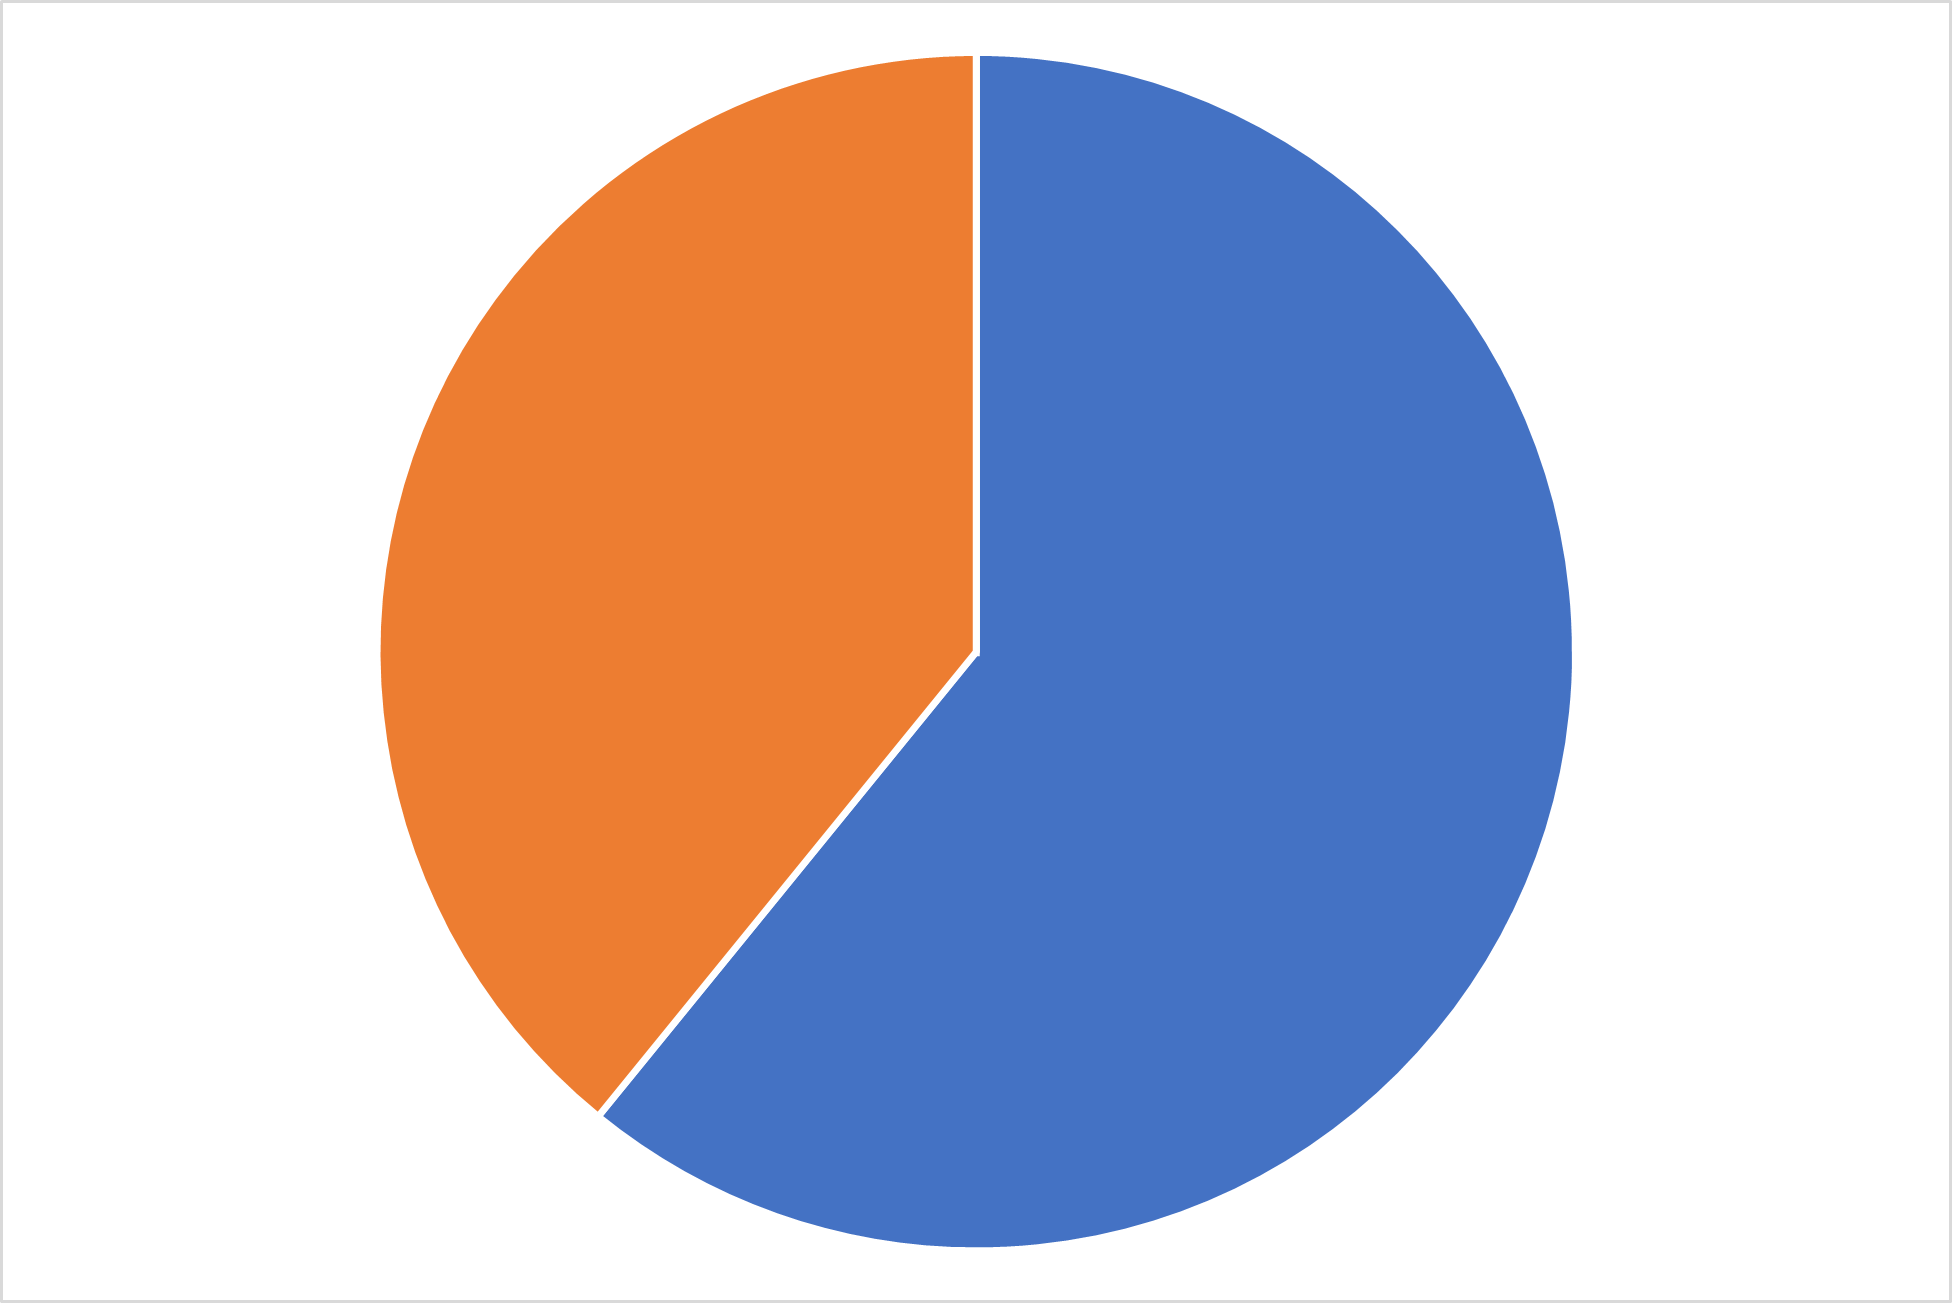
\includegraphics[width = 0.4\textwidth]{gfx/zufriedenheit-projekt-e.png}}
	\subfloat[Legende]{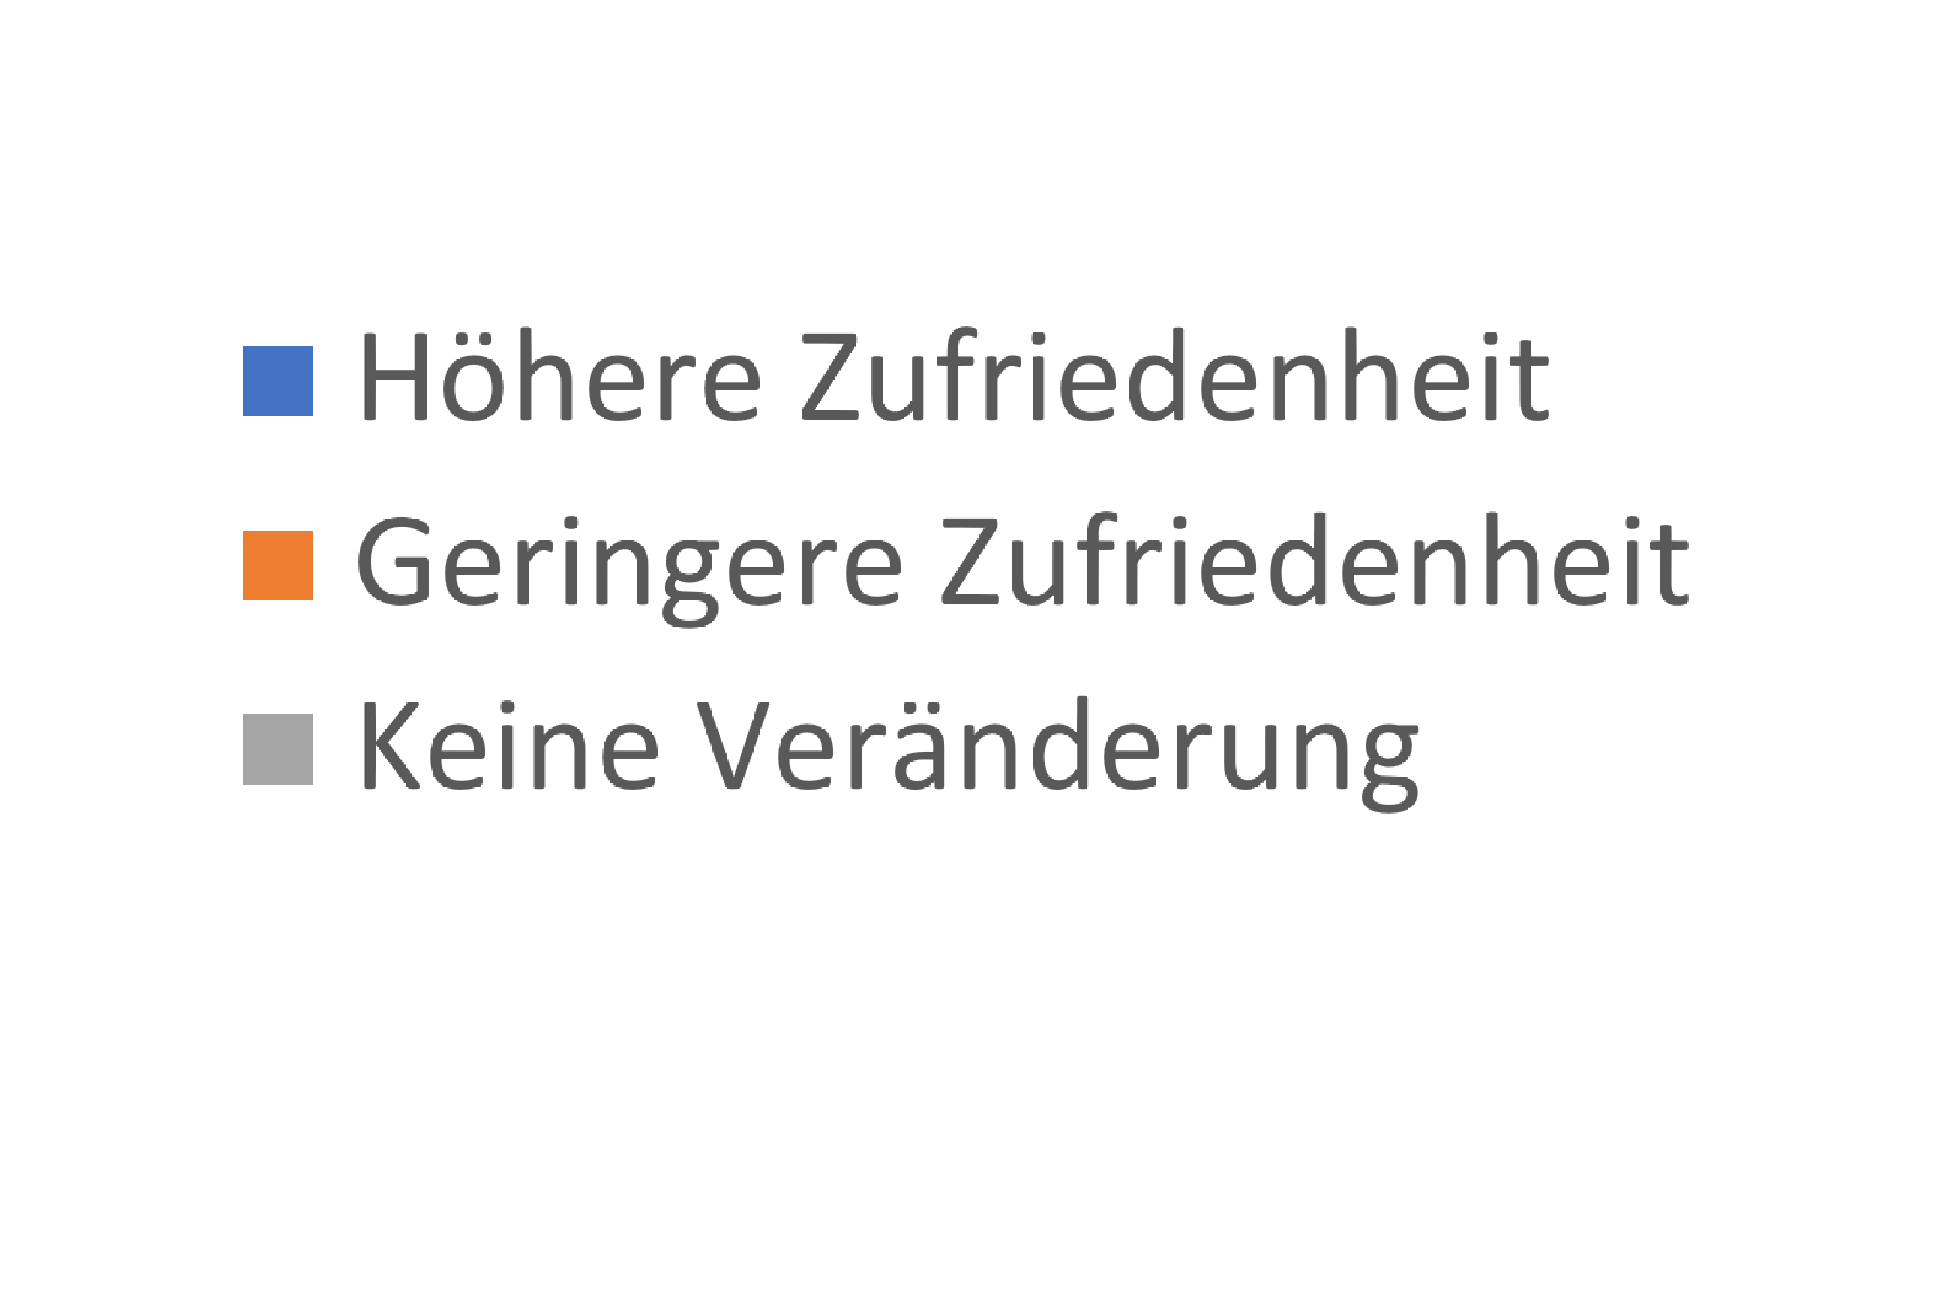
\includegraphics[width = 0.4\textwidth]{gfx/zufriedenheit-projekt-legende.png}}
	
	\caption{Ergebnisse des bilateralen Empfehlungsansatzes im Vergleich zum unilateralen Vorgehen hinsichtlich der Mitarbeiterzufriedenheit}
	\label{fig:ergebnisse:analyse:abb7}
\end{figure}

In Abbildung \ref{fig:ergebnisse:analyse:abb7} ist zu erkennen, dass der bilaterale Empfehlungsansatz einen Großteil der Angestellten für die Projektpositionen A und B zugunsten einer höheren Zufriedenheit positionierte. Bei den Projektpositionen D und E sind erreiche das bilaterale Vorschlagsverfahren für knapp über die Hälfte der Mitarbeiter eine höhere Zufriedenheit. Bei Projektposition C konnte dagegen der unilaterale Empfehlungsansatz für den Großteil der Angestellten eine höhere Zufriedenheit erzielen.

\subsection{Prognostizierte Arbeitsleistung der Projektmanager}
\label{ch:ergebnisse:fallstudie:arbeitsleistung}
\shorthandon{"}

\shorthandoff{"}
\chapter{Diskussion}
\label{ch:diskussion}

\section{Zusammenfassung der Forschungsergebnisse}
\label{ch:diskussion:zusammenfassung}
Im Rahmen der vorliegenden Master-Thesis wurde eine Fallstudie unter Projektmanagern und Mitarbeitern des IT-Beratungsunternehmens \mbox{EXXETA AG} durchgeführt. Dabei wurden die Vorschläge zur Besetzung offener Projektpositionen eines uni- und eines bilateralen Empfehlungsansatzes miteinander verglichen. Das bilaterale Vorschlagsverfahren konnte bei vier der fünf evaluierten Stellen eine höhere Zufriedenheit bei den Angestellten erzielen. Bei einer Projektposition sorgte dagegen der unilaterale Empfehlungsansatz für eine höhere Zufriedenheit. Vergleichbar fielen auch die Ergebnisse auf Seiten der Projektmanager aus. Hier prognostizierten die Verantwortlichen für drei der fünf Projektpositionen eine höhere Arbeitsleistung von den vorgeschlagenen Mitarbeitern des bilateralen Verfahrens. Bei zwei Stellen bewerten die Projektmanager dagegen die Arbeitsleistungen der vorgeschlagenen Angestellten der unilateralen Variante als höher.

Bei grafischer Darstellung von Präferenzen und beherrschten Fähigkeiten der befragten Mitarbeiter zeigte sich der sogenannte lange (Ratten-)Schwanz. Zudem hatten 17 Prozent der befragten Angestellten keine einzige Kompetenzbewertung im Intranet der EXXETA AG vorgenommen. Darüber hinaus konnte festgestellt werden, dass die Mitarbeiter einen Großteil ihrer präferierten Fähigkeiten nicht beherrschen. Weitere Analysen ergaben, dass etwa 28 Prozent der befragten Angestellten die durchschnittlich für eine offene Projektposition gesuchte Fähigkeit nicht als Präferenz angaben, obwohl sie diese beherrschen. 

Abschließend wurde evaluiert, wie Mitarbeiter und Projektmanager mit möglicher Unterforderung bei der Projektarbeit umgehen. Diesbezüglich konnte im Rahmen der Befragung festgestellt werden, dass sowohl Angestellte als auch Projektverantwortliche mehrheitlich eine Unterforderung vermeiden möchten.
\newpage
\section{Interpretation der Forschungsergebnisse}
\label{ch:diskussion:interpretation}
In Kapitel \ref{ch:personEnvironmentFit:auswirkungenErhoehterAngebote} wurde beschrieben, dass ein P-E Misfit in drei möglichen Konsequenzen mit entsprechenden Gleichungen zur Berechnung resultieren kann. Im Rahmen der vorliegenden Master-Thesis wurde angenommen, dass sowohl Projektmitarbeiter als auch -manager eine Unterforderung bei der Besetzung offener Projektpositionen vermeiden möchten. Dementsprechend wurde Kurve B aus Abbildung \ref{fig:personEnvironmentFit:auswirkungenErhoehterAngebote:abb1} in Form der quadrierten Differenzberechnung implementiert. Die im Rahmen der Fallstudie erhobenen Daten bestätigen diese Annahme sowohl aus Perspektive der Mitarbeiter als auch aus dem Blickwinkel der Projektverantwortlichen. 

Bei Implementierung der beiden Empfehlungsansätze wurde aufgrund der Erkenntnisse aus Kapitel \ref{ch:empfehlungssysteme} erwartet, dass sowohl der Kaltstart als auch der lange (Ratten-)Schwanz und das damit verbundene Sparsity Problem die Vorschlagserstellung beeinträchtigen würden. Daher lag den Empfehlungsmethoden ein hybrider und graphenbasierter Ansatz zugrunde, welcher über die Einbeziehung von Fähigkeitsbewertungen und Teamzuordnungen beide Probleme löste. Dieses Vorgehen ist mit Blick auf die Auswertung von beherrschten und präferierten Kompetenzen der Mitarbeiter als sinnvoll zu bewerten. Einerseits konnte in Abbildung \ref{fig:ergebnisse:analyse:abb1} der lange (Ratten-)Schwanz identifiziert werden und andererseits hatten 17 Prozent der befragten Mitarbeiter im Intranet keine einzige Fähigkeit bewertet.%Folglich wären diese Angestellten ohne Einbeziehung der Teamzuordnungen von einem Kaltstart betroffen.

Hinsichtlich der Kompetenzen konnte außerdem beobachtet werden, dass die Mitarbeiter einen Großteil ihrer präferierten Fähigkeiten nicht beherrschen. Aus diesem Sachverhalt lässt sich schließen, dass die Angestellten bereit sind, in Zukunft weitere Fähigkeiten zu erlernen und diese bei der Projektarbeit anzuwenden. Auf Unternehmensseite könnte dementsprechend der Einsatz zusätzlicher Weiterbildungsangebote evaluiert werden, bei welchen die Mitarbeiter nicht nur bestehende Kompetenzen vertiefen, sondern auch neue Fähigkeiten erlernen können.

Des weiteren zeigte die Auswertung der Mitarbeiterkompetenzen, dass das Beherrschen einer Fähigkeit keinen Rückschluss auf eine entsprechende Präferenz zulässt. Ein unilateraler Empfehlungsansatz würde dennoch sämtliche beherrschten Kompetenzen gleich behandeln. Somit ist davon auszugehen, dass die Angestellten bei Einsatz eines unilateralen Empfehlungssystems für Projektpositionen vorgeschlagen werden, deren gesuchte Fähigkeiten diese zumindest teilweise nicht anwenden möchten. Ein bilaterales System unterscheidet dagegen zwischen präferierten und nicht gewünschten Kompetenzen. Da dieser Ansatz präferierte Fähigkeiten stärker gewichtet, wird sich ein vorgeschlagener Mitarbeiter mit höherer Wahrscheinlichkeit die Anwendung der geforderten Kompetenzen wünschen. Dementsprechend ist eine höhere Zufriedenheit und Motivation bei der Stellenbesetzung zu erwarten. Diese Annahme spiegelt sich auch in den Ergebnissen der Umfragen unter den Mitarbeitern und Projektmanagern der EXXETA AG wider. Zur Verdeutlichung dieses Sachverhalts zeigt Abbildung \ref{fig:diskussion:interpretation:abb1} erneut die prognostizierte Zufriedenheit der Mitarbeiter mit den fünf vordefinierten Projektpositionen aus Kapitel \ref{ch:ergebnisse:fallstudie:umfrageMitarbeiter}.

\begin{figure}[h]
	\centering
	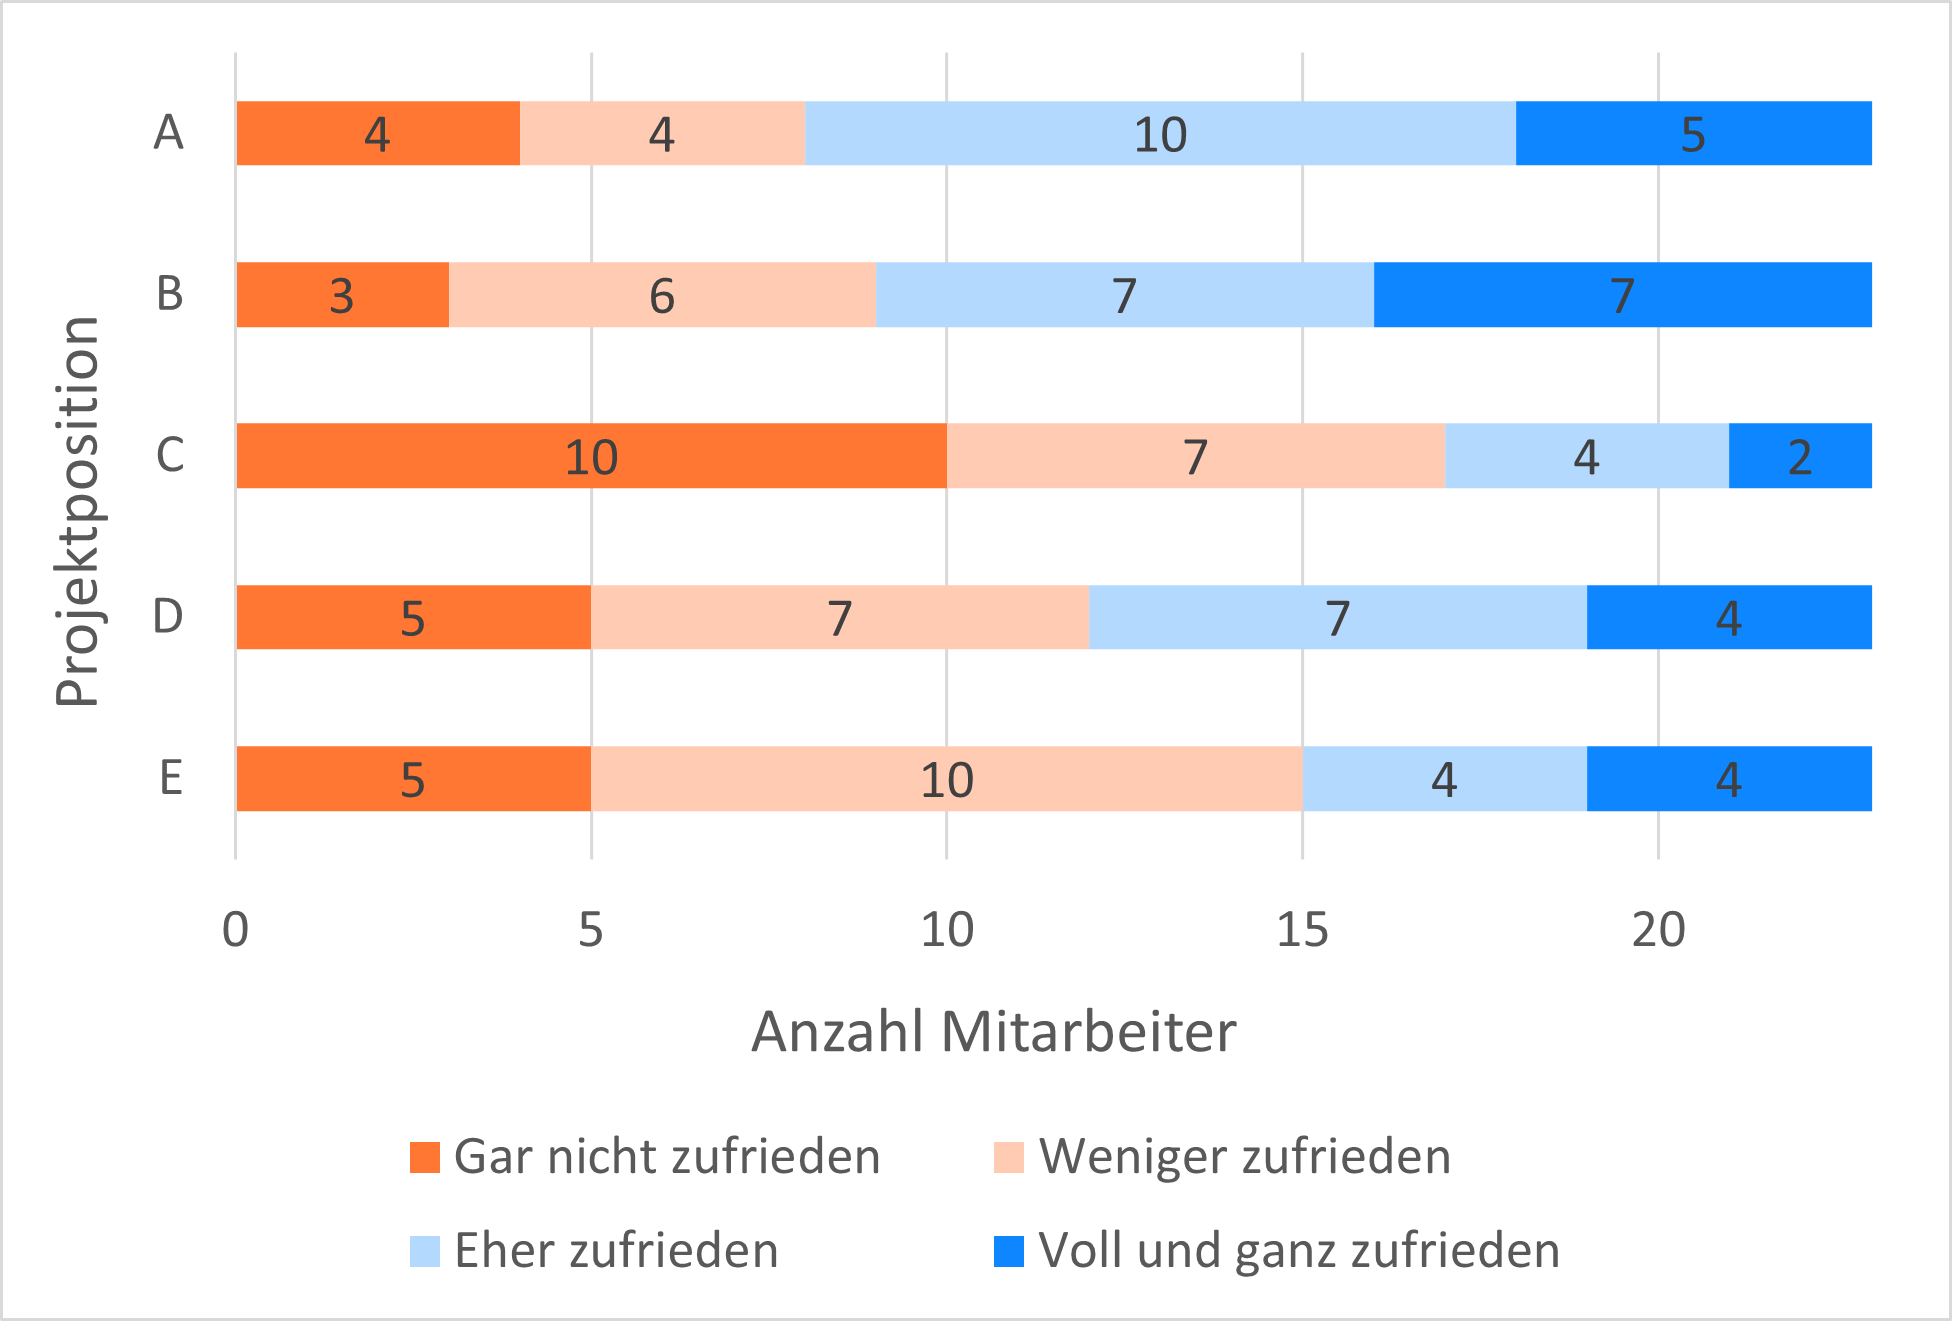
\includegraphics[width=0.925\textwidth]{gfx/mitarbeiter-zufriedenheit-umfrage.png}
	\caption{Anzahl an Mitarbeitern, welche zufrieden bzw. unzufrieden mit der Tätigkeit auf den jeweiligen vordefinierten Projektpositionen wären}
	\label{fig:diskussion:interpretation:abb1}
\end{figure}

Abbildung \ref{fig:diskussion:interpretation:abb3} veranschaulicht zusätzlich die Ergebnisse der uni- und bilateralen Empfehlungsansätze hinsichtlich der Mitarbeiterzufriedenheit. 

\begin{figure}[h]
	\centering
	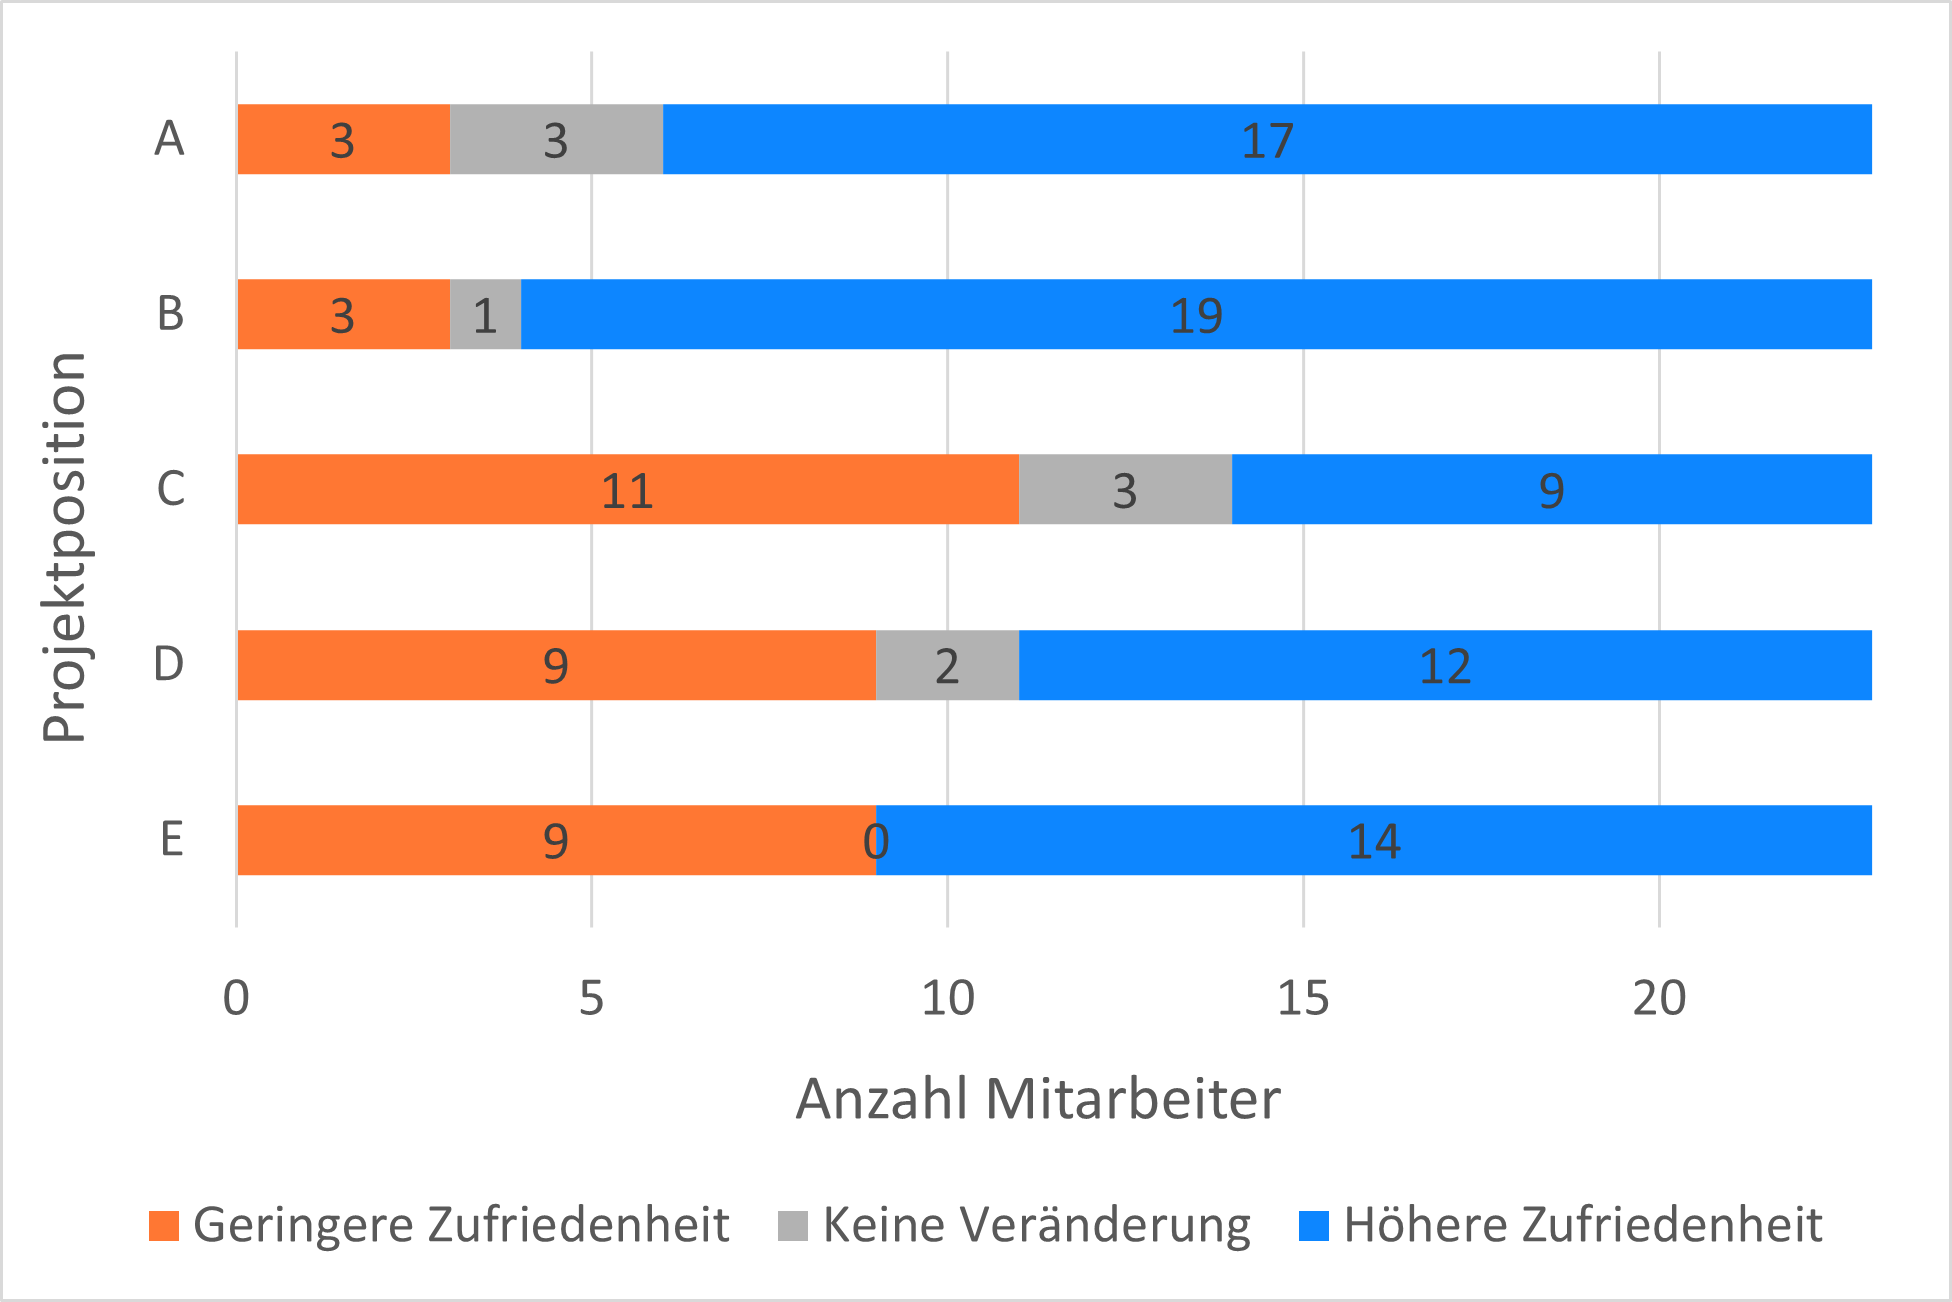
\includegraphics[width=0.925\textwidth]{gfx/zufriedenheit-projekte.png}	
	\caption{Ergebnisse des bilateralen Empfehlungsansatzes im Vergleich zum unilateralen Vorgehen hinsichtlich der Mitarbeiterzufriedenheit}
	\label{fig:diskussion:interpretation:abb3}
\end{figure}

In den Abbildungen \ref{fig:diskussion:interpretation:abb1} und \ref{fig:diskussion:interpretation:abb3} ist zu erkennen, dass die Mitarbeiter durch den bilateralen Empfehlungsansatz stärker zu deren Zufriedenheit positioniert werden, wenn sie eine hohe Akzeptanz mit der Stelle prognostizieren. Dieser Sachverhalt ist insbesondere bei den Projektpositionen A und B zu beobachten, für welche über die Hälfte der Mitarbeiter in Abbildung \ref{fig:diskussion:interpretation:abb1} eine hohe Präferenz angaben. Hier ordnete der bilaterale Empfehlungsansatz in Darstellung \ref{fig:diskussion:interpretation:abb3} etwa dreiviertel aller Angestellten gegenüber der unilateralen Variante stärker zu deren Zufriedenheit an. Zeigen dagegen weniger Mitarbeiter Gefallen an einer betrachteten Stelle, nimmt auch die Qualität des bilateralen Empfehlungsansatzes hinsichtlich der Mitarbeiterzufriedenheit ab. Besonders gut ist diese Begebenheit bei Projektposition C zu erkennen, mit welcher sich die Mitarbeiter in Abbildung \ref{fig:diskussion:interpretation:abb1} mehrheitlich unzufrieden zeigen. Hier erzielte der bilaterale Empfehlungsansatz in Grafik \ref{fig:diskussion:interpretation:abb3} im Vergleich zur unilateralen Variante sogar Ergebnisse, welche zu einer geringeren Akzeptanz bei den Mitarbeitern führen.

Ähnliche Ergebnisse können auch für die Perspektive der Projektmanager abgeleitet werden. Abbildung \ref{fig:diskussion:interpretation:abb4} zeigt die Resultate der Umfrage unter den Projektverantwortlichen hinsichtlich der erwarteten Arbeitsleistung der Angestellten.

\begin{figure}[h]
	\centering
	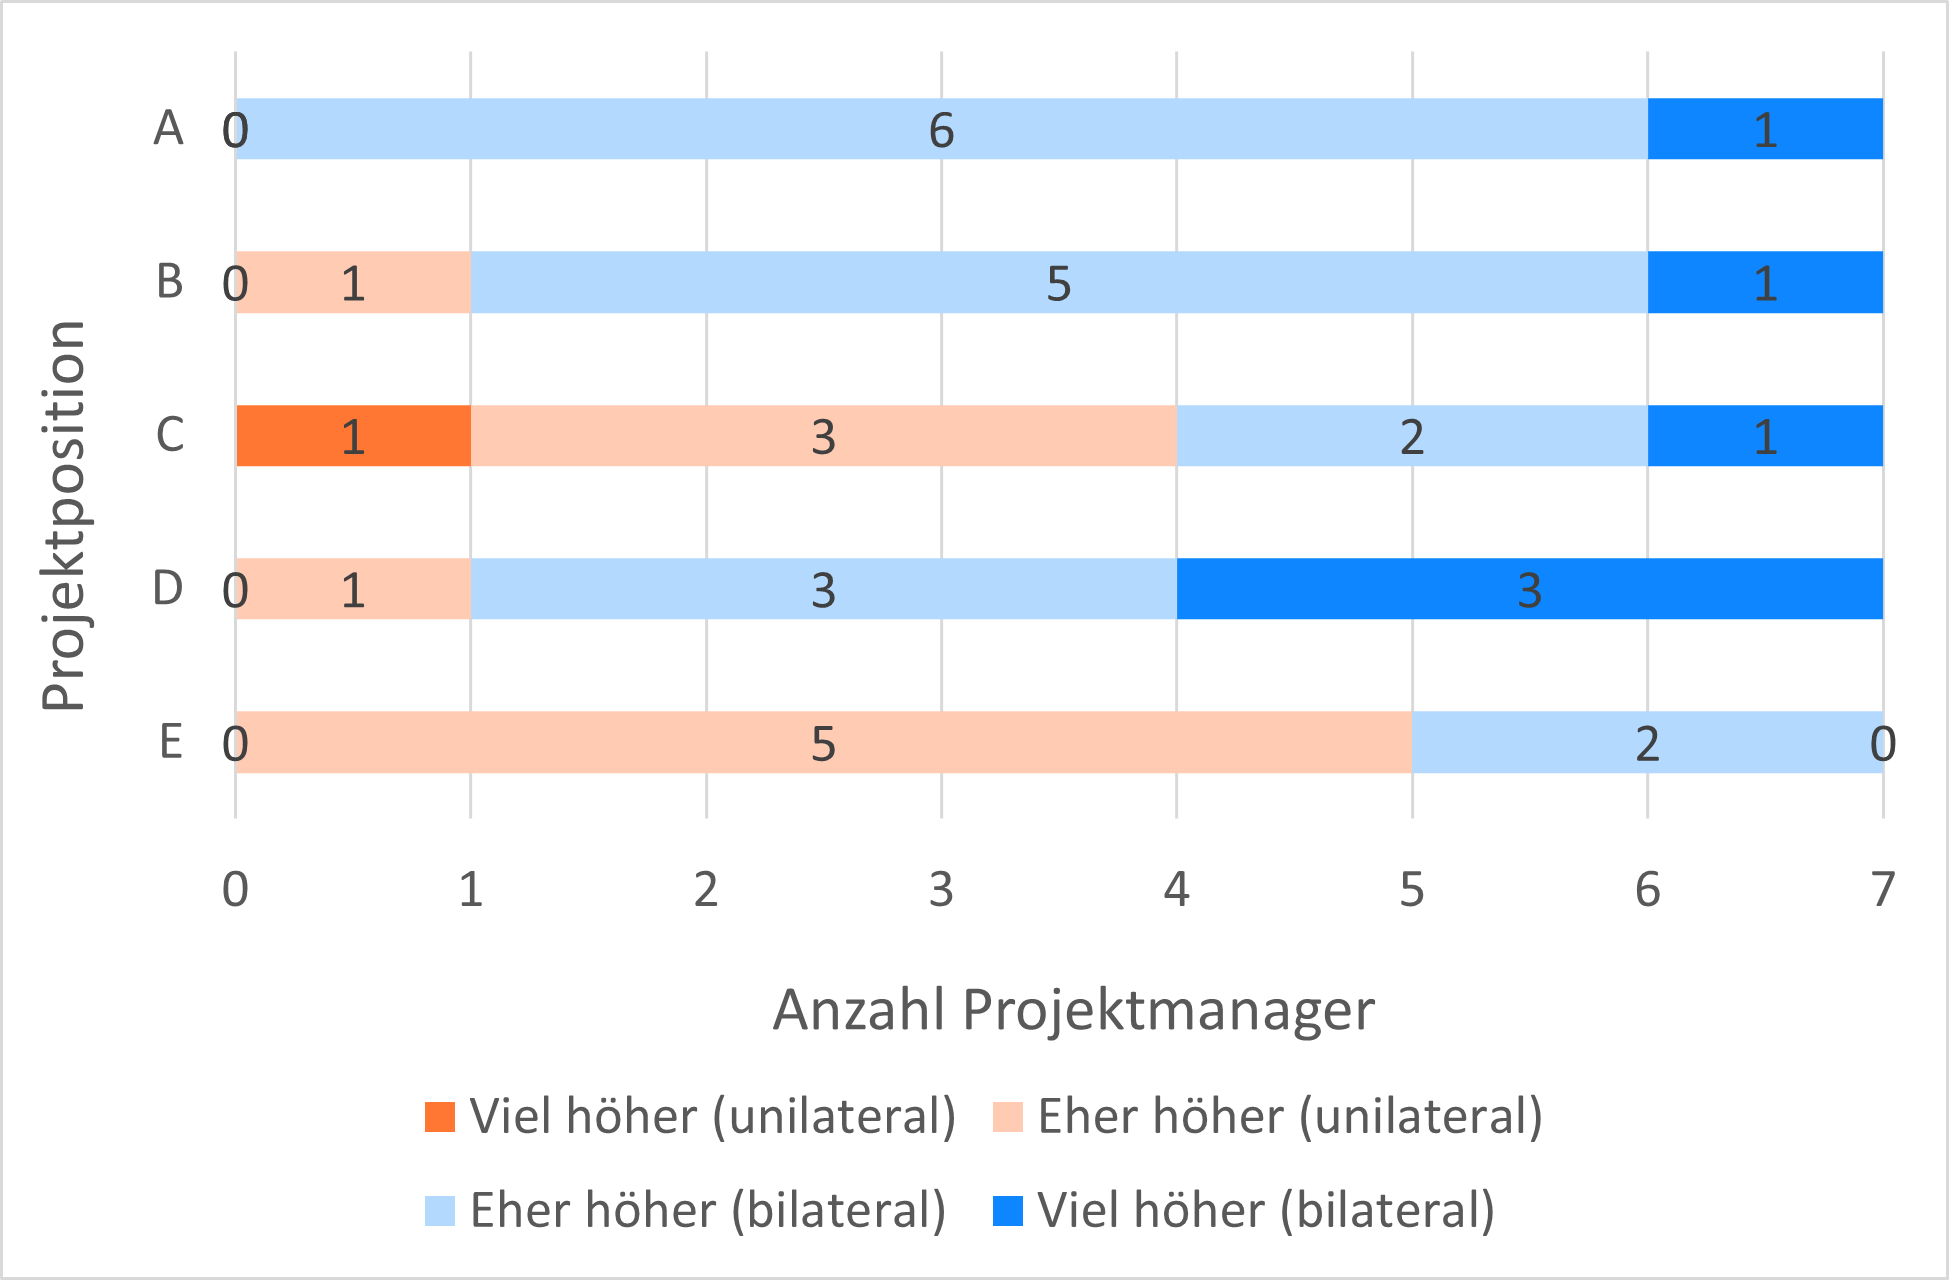
\includegraphics[width=0.925\textwidth]{gfx/ergebnisse-projektmanager-arbeitsleistung.png}	
	\caption{Ergebnisse der Umfrage unter den Projektmanager hinsichtlich der erwarteten Arbeitsleistung der Mitarbeiter}
	\label{fig:diskussion:interpretation:abb4}
\end{figure}

In Abbildung \ref{fig:diskussion:interpretation:abb4} ist für die Projektpositionen A und B zu beobachten, dass die Projektmanager eine höhere Arbeitsleistung von den Vorschlägen des bilateralen Empfehlungsansatzes erwarten. Hierbei handelt es sich um die Stellen, mit welchen sich auch ein Großteil der Mitarbeiter in Abbildung \ref{fig:diskussion:interpretation:abb1} zufrieden zeigen. Für die Projektpositionen C und E, mit welchen die Angestellten in Darstellung \ref{fig:diskussion:interpretation:abb1} mehrheitlich unzufrieden sind, erwarten die Projektmanager eine geringere Leistung von den Vorschlägen des bilateralen Empfehlungsansatzes.

Dementsprechend wird aus den Ergebnissen der Fallstudie geschlossen, dass der bilaterale Empfehlungsansatz im Vergleich zur unilateralen Variante immer dann für eine höhere Zufriedenheit bei den Angestellten und für eine gesteigerte erwartete Arbeitsleistung unter den Projektmanagern sorgt, wenn die Mitarbeiter mehrheitlich eine hohe Akzeptanz mit der betrachteten Stelle zeigen. Eine Ausnahme von dieser Regel bildet lediglich Projektposition D in Abbildung \ref{fig:diskussion:interpretation:abb4}. Hier sorgten die Vorschläge des bilateralen Empfehlungsansatzes aus Perspektive der Projektmanager für eine wesentlich höhere prognostizierte Arbeitsleistung, obwohl sich die Mitarbeiter in Darstellung \ref{fig:diskussion:interpretation:abb1} mehrheitlich unzufrieden mit der Stelle zeigten. Wie in Abbildung \ref{fig:diskussion:interpretation:abb2} zu erkennen, unterschieden sich die Vorschläge zu Projektposition D in der Umfrage unter den Projektmanagern jedoch in nur einer Person.

\begin{figure}[h]
	\centering
	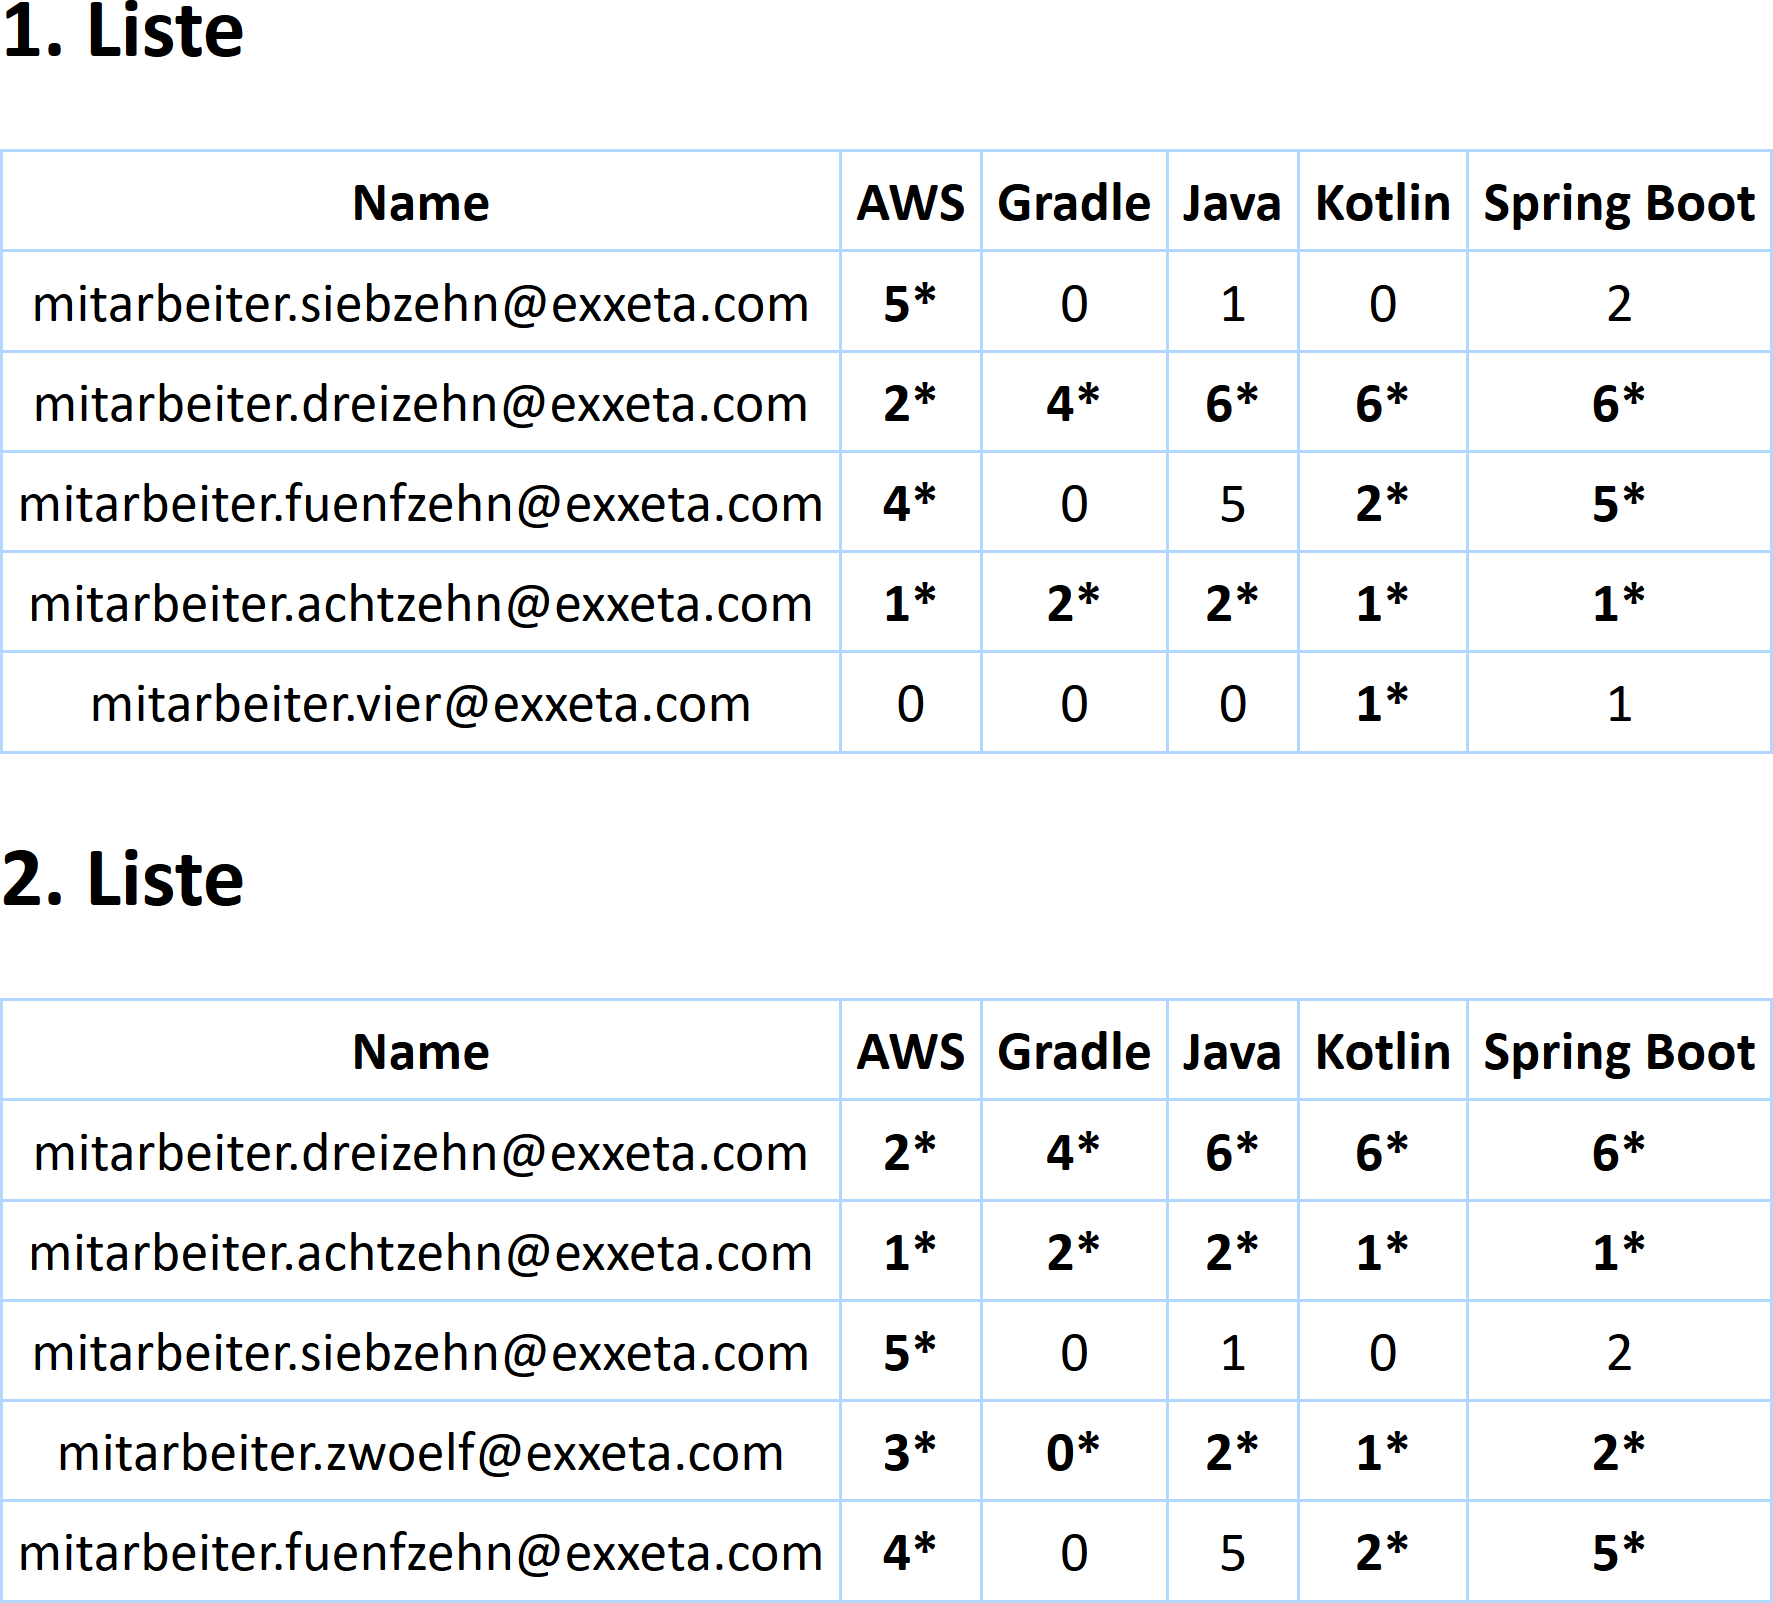
\includegraphics[width=0.75\textwidth]{gfx/projektposition-d.png}
	\caption[Mitarbeiter-Vorschläge für Projektposition D in der Umfrage unter den Projektmanagern]{Mitarbeiter-Vorschläge für Projektposition D in der Umfrage unter den Projektmanagern\\
	(Klarnamen wurden aus Datenschutzgründen nachträglich pseudonymisiert)}
	\label{fig:diskussion:interpretation:abb2}
\end{figure}

Aufgrund des geringen Unterschieds in den Vorschlägen aus Abbildung \ref{fig:diskussion:interpretation:abb2} werden die Ergebnisse der Projektverantwortlichen für Projektposition D als nicht repräsentativ betrachtet, sodass sie die erlangten Erkenntnisse der vorliegenden Master-Thesis nicht widerlegen.

Somit ist zusammenfassend festzustellen, dass der bilaterale Empfehlungsansatz für eine höhere Zufriedenheit der Angestellten und eine gesteigerte erwartete Arbeitsleistung seitens der Projektmanager sorgt, wenn die Mitarbeiter mehrheitlich eine hohe Präferenz für eine betrachtete Projektposition aufweisen.

Als Ursache für diese Einschränkung wird die Art der Erhebung der Präferenzen betrachtet. Die Mitarbeiter gaben im Rahmen dieser Master-Thesis ihre Wünsche über boolesche Werte an. Hierbei gewichtete der bilaterale Empfehlungsansatz die präferierten Fähigkeiten der Angestellten höher. Es wurde jedoch nicht unterschieden, ob ein Angestellter einer nicht gewünschten Kompetenz neutral gegenübersteht oder ob er diese nicht bei der Projektarbeit anwenden möchte.

Aufgrund dieser Einschränkung wird für folgende Arbeiten empfohlen, den im Rahmen dieser Arbeit implementierten Empfehlungsansatz zu erweitern. Hierbei sollten die Präferenzen nicht über boolesche Werte, sondern über Abstufungen der Form "möchte ich anwenden", "neutral", "möchte ich nicht anwenden" erhoben werden. Bei der Implementierung sollten die Mitarbeiter bei vorhandenem Wunsch weiterhin höher positioniert und bei einem negativen Wert zusätzlich niedriger einsortiert werden. Unter Betrachtung dieser Veränderungen sollte die Evaluation unter Angestellten und Projektmanagern nochmals durchgeführt und die Forschungsfrage erneut untersucht werden.

\section{Einordnung in die Literatur und Ausblick}
\label{ch:diskussion:einordnung}
Bislang betrachten Empfehlungssysteme im Bereich der Personalauswahl Problemstellungen laut \textcite[S. 1ff.]{malinowski:2006} zumeist entweder aus Perspektive der Personalverantwortlichen oder aus dem Blickwinkel der Mitarbeiter. Dieses Vorgehen verfolgte im Rahmen der vorliegenden Arbeit auch die unilaterale Empfehlungskomponente, welche ausschließlich die Präferenzen der Projektmanager betrachtete. Obwohl die bilaterale Variante zusätzlich die Wünsche der Mitarbeiter einbezog und somit die Vorschläge des unilateralen Systems verzerrte, verbesserten sich die gemessenen Ergebnisse für die Mehrheit der Projektpositionen sowohl auf Seiten der Mitarbeiter als auch aus Perspektive der Projektmanager. Somit zeigt die vorliegende Master-Thesis, dass die Erkenntnisse von \textcite[S. 5ff.]{parsons:1909} aus dem Jahr 1909 bzw. \textcite[S. 11f.]{lewin:1936} und \textcite[S. 38ff.]{murray:1938} aus den 1930er-Jahren zum Zusammenwirken von Person und Umgebung noch heute aktuell sind und sich auch auf die Implementierung von Empfehlungssystemen übertragen lassen. Diese Erkenntnis sollten zukünftige Arbeiten bei der Entwicklung von Vorschlagsverfahren in den Bereichen der Personalauswahl und der Stellensuche berücksichtigen. Für diese Problemstellungen entwickelte Systeme sollten ihren Fokus dementsprechend von der getrennten Betrachtung von Person und Umgebung verstärkt auf das Zusammenspiel beider Komponenten richten. 
\shorthandon{"}
\shorthandoff{"}
\chapter{Fazit (WIP)}
\label{ch:fazit}
\section{Fazit}
\label{ch:fazit:fazit}
- Ob man die Anforderungen der Stelle erfüllt, ist dem Mitarbeiter eigentlich egal. Ihn interessiert es nur, ob dadurch seine Werte verstärkt/erfüllt werden. Es wäre also interessant, herauszufinden, wieso ein Mitarbeiter z.B. mehr Python anwenden würde. Mehr Gehalt wegen Data Science? Neugier für neue Sprache? Kumpel arbeitet in dieser Abteilung? ... \\
- Eigentlich müsste der Prozess des Motivations-Herausfindens dem kompletten Einstellungsprozess vorgelagert sein \note{Kann sich die Motivationslage nicht ändern?}. Bzw. sogar dem Studium \\
- Grenze: \textcite{cable:1997} stellten fest, dass das Bauchgefühl des Interviewers besser vorhersagen kann, ob eine P zur O passt. Wenn also ein Unternehmen so klein ist, dass der "Staffer" alle Berater persönlich kennt, kann er wahrscheinlich besser zuordnen als die KI \\
- Anmerkung von mir: Während \textcite{parsons:1909} 1909 also noch davon ausging, dass alles möglichst objektiv und wissenschaftlich korrekt gemessen werden muss, gehen Psychologen heute davon aus, dass primär die subjektive Wahrnehmung eine Hauptrolle spielt \\
- Subjektive Wichtigkeiten bewerten wie bei Story-Points in Scrum

\section{Fragen}
\label{ch:fazit:fragen}
- Die historischen Bücher sprechen immer nur von "Männern" --> kann man daraus einfach "Menschen" machen?\\ \note{Zitattechnisch: Nein. Auch inhaltlich ist das eine spannende Frage. Für Motivationslagen spielen soziale, kulturelle und gesellschaftliche Aspekte ja eine Rolle.}
- Gründungsvater ist ein englisches Zitat --> Wie zitieren?\\ \note{Üblich ist das Orginalzitat mit zusätzlicher Übersetzung}
- Wie umgehen mit den englischen Begriffen? z.B. fit, Need, Desire, etc. \note{Ggf. als Eigenbegriffe nutzen}

\section{Anmerkungen}
\label{ch:fazit:anmerkungen}
- "Referent" klingt komisch (Christian)\\
- Zweite Seite und "I. Thesis" ist unnötig (Christian)\\
- JSON und REST im Abkürzungsverzeichnis muss nicht sein (Christian)\\
- Wort: "Fallstudie" (Christian)\\
- Forschungsfrage: Symmetrische sollte klarer formuliert werden --> Kommt etwas hinterher --> Eher an den Anfang (Andreas)\\
- Forschungsfrage ist sehr lang (Christian)\\
- Einleitung: Warum erhöht die dezentrale Kommunikation die Kreativität? (Christian)\\
- Zu Empfehlungssystemen: Könnten wir uns nicht auf einen Teilgraphen beschränken? (Jan)\\
- Verlinkungen z.B. PE-Fit unterstreichen? (Nina)\\
- Formel \ref{frml:verwandteArbeiten:formel1} raus? (Nina)\\
- Bilddiskussion in Kapitel \ref{ch:verwandteArbeiten:aufDemPEFitBasierendeBilateraleSysteme:pjUndPtFit} in Präsens? (Nina)\\
- \ref{ch:verwandteArbeiten:aufDemPEFitBasierendeBilateraleSysteme:bilateraleVertrauensbestimmung}: Was ist an der Formel noch nicht optimal? (Nina)\\
- Zeile (Z) bei wörtlichen Zitaten aufnehmen? (Christian)\\
- Historischer Teil bei \ac{PEFit} ist unnötig, um Thesis zu verstehen - nur nice-to-know (Christian)\\
- Viel "die Wissenschaftler" (Christian)\\
- Bilder im \ac{PEFit}-Kapitel auf deutsch und dann englische Begriffe im Fließtext weglassen / Auch Long Tail-Bild auf deutsch (Christian)\\
- Ist \ref{fig:personEnvironmentFit:auswirkungenErhoehterAngebote:formel4} notwendig? (Christian)\\
- Qualität von \ref{fig:personEnvironmentFit:wichtigkeiten:abb2} könnte besser sein (Christian)\\
- "e-lancer", P-E Misfit, Pearson Korrelation, Sparsity Problem und Recommender Engine kursiv? (Christian)\\
- Aufkommen der Recommender Engines, YouTube, Filterblase --> an der Grenze, ob es relevant ist (Christian)\\
- Ist es häufig so, dass man direkte Treffer hat oder dass man indirekte Treffer hat? --> Sucht man nach verbreiteten Skills oder nach exotischem? --> Einfach nur als Beobachtung (Andreas)\\
- S. 22: Nicht nur die Skalierung ist verändert --> Verhältnisse --> Relative Werte verändern sich / Statt Skalierung: Glättung - dazu sollten noch 1-2 Sätze rein und das erklären und noch ein Argument dazu rein, warum das kein Problem ist, sondern wieso das vielleicht sogar gut ist (Andreas)\\
- Ontologien für Skills (Johannes)\\
- Rechtschreibfehler in Skills (Johannes)\\
- Abkürzungen nicht eindeutig (Imanuel)
\shorthandon{"}
%\shorthandoff{"}
\chapter{Notizen}
\label{ch:notizen}

\section{Gliederung}
\label{ch:notizen:gliederung}

\begin{enumerate}
    \item Einführung
%    \item Empfehlung von Personen (Zuordnung Person-Umgebung): Verweisen auf Thesis Johannes und nur Unterteilung PE-Fit in Skill-Match, Job-Match und Organizational-Match erklären ?
    \item Empfehlungssysteme
    \begin{itemize}
        \item Allgemeine Problemstellung
        \item Vorgehen (Prediction und Ranking)
        \item Präferenzen in Empfehlungssystemen (nicht personalisiert vs. personalisierte Systeme) -> Präferenzen in unserem Anwendungsfall: Attribute der Mitarbeiter
        \item Erweiterungen von Empfehlungssystemen: Fokus auf Multicriteria-Rating in Empfehlungssystemen -> Einbeziehen mehrerer Kriterien für die Empfehlungsbestimmung % Überleitung zu RRS: Wie funktioniert die Berücksichtigung wechselseitiger Präferenzen? d.h. dass nicht nur Präferenzen der Nutzer, sondern in unserem Fall der Elemente mit aufgenommen werden können?
    \end{itemize}
    \item Reciprocal Recommenders: Sowohl Präferenzen der Nutzer, als auch Präferenzen der Elemente, die empfohlen werden, werden in Empfehlung miteinbezogen % S.9: file://wsl%24/Ubuntu/home/masc6/Projects/masterarbeit/literatur/Recommender%20Systems%20for%20Online%20Dating.pdf
    \item Verwandte Arbeiten (Arbeiten über die Verwendung von Präferenzen auf Element-Seite für Ermittlung von Empfehlungen)
    \item Methodik (Ansatz und Umsetzung)
    \item Evaluation
    \item Diskussion
    \item Fazit
\end{enumerate}

\newpage

\section{Einführung: Relevanz und Motivation}
\label{ch:notizen:relevanzMotivation}
Warum ist das Thema relevant?
\begin{itemize}
    \item Einstieg: People are social creatures—fundamentally so. We look for other people for a multitude of purposes: dating and eventually marriage, pursuing shared interests, addressing community issues, solving technical problems, or maybe just having a good conversation.% S. 401, 
    \item Einstieg: Unternehmen arbeiten zunehmend projektbasiert. Zuordnung von Personen zu Jobpositionen ist folglich Aufgabe in vielen Unternehmen.
    \item Personen und Jobs die nicht zusammenpassen bedeuten für Unternehmen Aufwand (Kosten, Zeit, Qualitätseinbuße, Unzufriedenheit).
    \item Nicht nur im Recruiting relevant, sondern auch innerhalb von Organisationen % (http://www.timothy-judge.com/Cable%20&%20Judge%20OBHDP%201996.pdf). Dort steckt viel Potenzial.)
    \item Daher: Berücksichtigen diverser Attribute von Personen und Umgebung bei der Auswahl von Personen für Berufe/Jobpositionen (d.h. weg vom alleinigen skill matching zum job matching).
    \item Dadurch soll die Performance der Mitarbeiter im Job, sowie deren Mitarbeiterzufriedenheit gesteigert werden.
    \item Empfehlungssysteme, um bei der Entscheidung der Wahl von Personen zu Jobpositionen zu unterstützen (Decision Support) % S.77, file://wsl%24/Ubuntu/home/masc6/Projects/masterarbeit/literatur/E-Commerce.pdf
\end{itemize}

\section{Empfehlungssysteme}
\textbf{Einführung: Begrifferklärungen, Warum Empfehlungssysteme?}\\
Warum Empfehlungssysteme? Zur Verfügung stellen einer sortierten teilmenge an elementen, in Abhängigkeit der angenommenen Relevanz für Nutzer. % S. 76, file://wsl%24/Ubuntu/home/masc6/Projects/masterarbeit/literatur/E-Commerce.pdf
Relevanz ist gegeben durch explizites bzw. implizites Feedback eines Nutzers bzw. einer Gruppe an Nutzern. % S. 76, file://wsl%24/Ubuntu/home/masc6/Projects/masterarbeit/literatur/E-Commerce.pdf
Bestandteile eines Recommender Systems erklären: user model, community, item model, recommender algorithm und interaction style, Erklärung Nutzer, Element, Nutzer-Element-Kombination.\\ % S. 8:1 (file://wsl%24/Ubuntu/home/masc6/Projects/masterarbeit/literatur/Modeling%20User%20Preferences%20in%20Recommender%20Systems.pdf)

Auswahl der Elemente, sodass der Nutzen für den Nutzer maximal ist.
Formal ausgedrückt soll in einem Empfehlungssystem einem Nutzer $c$ eine Menge an Elementen $s'$ $\in$ $S$ empfohlen werden, für die gilt:
\begin{equation} % S. 49, file://wsl%24/Ubuntu/home/masc6/Projects/masterarbeit/literatur/New_Recommendation_Techniques_for_Multicriteria_Rating_Systems.pdf
    \forall c\in C,  s'_c = arg\max_{s \in S} R(c,s)
\end{equation}
wobei $C$ die Menge aller Nutzer und $S$ die Menge aller möglichen Elemente angibt.

Der Nutzen kann über die Nutzenfunktion $R(c,s)$ bestimmt werden und gibt als Ergebnis den (angenommenen) Wert einer Nutzer-Element-Kombination zurück.
% Hier noch hinzufügen, dass in RS das Ergebnis der funktion u sowohl unmittelbar aus expliziten oder implizitem feedback bestehen kann, als auch einer vorhersage
Die Nutzenfunktion $R$ ist definiert als % file://wsl%24/Ubuntu/home/masc6/Projects/masterarbeit/literatur/New_Recommendation_Techniques_for_Multicriteria_Rating_Systems.pdf , S. 847, file:///C:/Users/masc6/OneDrive/Persoenliche_Unterlagen/Uni/Masterthesis/2015_Book_RecommenderSystemsHandbook.pdf
\begin{equation}
    R: Nutzer \times Element \rightarrow R_{0}
\end{equation}
wobei $R_{0}$ die Menge aller Werte darstellt, die ein Rating annehmen kann (z.B. ganze Zahlen von  1 bis 5). % S. 847, file:///C:/Users/masc6/OneDrive/Persoenliche_Unterlagen/Uni/Masterthesis/2015_Book_RecommenderSystemsHandbook.pdf , file://wsl%24/Ubuntu/home/masc6/Projects/masterarbeit/literatur/New_Recommendation_Techniques_for_Multicriteria_Rating_Systems.pdf

\textbf{Vorgehen: Wie funktionieren Empfehlungen allgemein?}
\begin{itemize}
    \item Erklärung, wie Empfehlungen allgemein bestimmt werden (2 Teilschritte).
    \item Allgemein erfolgt die Empfehlung von Nutzern bzw. Elementen in Empfehlungssystemen in zwei Teilschritten: % Erklärung S. 405 unten: https://link.springer.com/content/pdf/10.1007/s11577-021-00753-z.pdf
    \begin{enumerate}
        \item Vorhersage unbekannter Nutzer-Element-Kombinationen (Rating - Prediction - Phase) % Phasen siehe S. 854, file:///C:/Users/masc6/OneDrive/Persoenliche_Unterlagen/Uni/Masterthesis/2015_Book_RecommenderSystemsHandbook.pdf
        \item Ranking und Ausgabe der Top-K-Nutzer (Recommendation - Generation - Phase) % Ranking als Key-Functionality von match-making systems -> S. 66: file://wsl%24/Ubuntu/home/masc6/Projects/masterarbeit/literatur/DiazMetzlerAmer-Yahia%20-%20Relevance%20and%20Ranking%20in%20Online%20Dating%20Systems%20(2010)%20-%200.pdf
    \end{enumerate}
\end{itemize}
% 1. schritt geht davon aus, dass Daten zu Attributen unvollständig sind und daher vorhergesagt werden müssen
% 2. Schritt ist dann die Bestimmung der passenden Mitarbeiter und der Ausgabe der Empfehlung (damit wird sich in der Arbeit befasst)

\textbf{Präferenzen in Empfehlungssystemen: Wie werden Präferenzen von Nutzern in Empfehlungen miteinbezogen?}\\
Erklären, was mit Präferenzen in Empfehlungssystemen im allgemeinen Sinn gemeint ist -> Präferenzen des Nutzers (Purchase history, ...) % S. 852, user preferences als purchase history: file:///C:/Users/masc6/OneDrive/Persoenliche_Unterlagen/Uni/Masterthesis/2015_Book_RecommenderSystemsHandbook.pdf
key indicator für preferences stellt explizites und implizites rating dar. % S.1, file://wsl%24/Ubuntu/home/masc6/Projects/masterarbeit/literatur/Modeling%20User%20Preferences%20in%20Recommender%20Systems.pdf
Unterscheidung von RS in personalisierte und nicht-personalisierte Empfehlungssysteme % file://wsl%24/Ubuntu/home/masc6/Projects/masterarbeit/literatur/Die%20Ordnung%20von%20Empfehlungen.pdf
\begin{itemize}
    \item nicht-personalisierte / schwach-personalisierte Empfehlungssysteme (Popularitätsmetriken, z.B. "Top 10 Songs in Deutschland", "Am häufigsten gekauft")
    \item personalisierte Empfehlungssysteme ("Songs für dich", "Das könnte dich auch interessieren")-> hier werden Präferenzen im eigentlichen Sinn miteinbezogen
\end{itemize}

Im Regelfall werden Präferenzen von Nutzern in personalisierten Empfehlungssystemen dafür verwendet, Beziehungen zwischen Nutzern und Elementen vorherzusagen.
Im vorliegenden Anwendungsfall stellen Projekte die Nutzer dar und Mitarbeiter die Elemente, die auf Projekte zugeordnet werden können.
Bei den angegebenen Präferenzen handelt es sich um ein Attribut des Mitarbeiters, und zwar in Form einer Bewertung der Fähigkeiten im System durch die Mitarbeiter.

Der Unterschied liegt also darin, dass im vorliegenden Anwendungsfall die Elemente Präferenzen besitzen, nicht, wie in klassischen Empfehlungssystemen die Nutzer. % S. 852, user preferences als purchase history: file:///C:/Users/masc6/OneDrive/Persoenliche_Unterlagen/Uni/Masterthesis/2015_Book_RecommenderSystemsHandbook.pdf
Noch ein Unterschied: Nutzer, d.h. in unserem Fall Projekte, haben keine vergangenen Nutzer-Element-Kombinationen, sondern nur einmalig, daher wird nicht basierend auf vergangenem auf zukünftiges geschlossen, sondern lediglich auf Basis des aktuellen Stands eine Empfehlung ermittelt.

Das bedeutet, damit die Präferenzen berücksichtigt werden können, muss ermittelt werden, wie Präferenzen von Elementen in die Bestimmung von Empfehlungen miteinbezogen werden können.

Frage: Sollen die Präferenzen der Mitarbeiter (Like, Dislike) als separate Attribute betrachtet werden? -> das würde dann in die Richtung der verschiedenen Ausprägungen des PE-Fit gehen (in diesem Fall Anforderungen-Fähigkeiten-Fit und Angebot-Bedürfnisse-Fit). Das Ergebnis der Fits würde dann kombiniert werden und gemeinsam den PE-Fit ergeben. Der PE-Fit würde sich dann also aus einer Kombination der einzelnen Fits ergeben. Würde man den PE-Fit zukünftig noch genauer ermitteln wollen, liesen sich in dieser Darstellung recht verständlich neue Attribute hinzufügen (z.B. Kapazität).
Oder sollen die Präferenzen unmittelbar den Wert einer Fähigkeit beeinflussen (d.h. wie in Johannes Thesis bedeutet 1 Like zb addition eines wertes und ein dislike Abzug o.Ä.)?

\textbf{Erweiterterungen von Empfehlungssystemen}\\
mehrere Erweiterungen, u.A.: Multicriteria Rating. % file://wsl%24/Ubuntu/home/masc6/Projects/masterarbeit/literatur/Toward_the_next_generation_of_recommender_systems_a_survey_of_the_state-of-the-art_and_possible_extensions.pdf

Für uns interessant: Multicriteria-Rating.
% MCRS als eine der Herausforderungen von Empfehlungssystemen der nächsten Ära. S. 1157, file://wsl%24/Ubuntu/home/masc6/Projects/masterarbeit/literatur/A_Review_and_Classification_of_Multi-Criteria_Recommender_Systems.pdf

% Erklärung, dass für die Lösung der Forschungsfrage der zweite Schritt relevant ist
\textbf{Gesucht:} Wert des Matches (= Rating) zwischen Nutzer und Element (Projekt und Mitarbeiter)\\
Die Frage ist also: wie kann das Rating berechnet werden, wenn die Präferenzen von Elementen einbezogen werden sollen?\\

\textbf{Multicriteria-Rating:}\\
% Aggarwal S. 426!
In den meisten RS bestimmt die Nutzenfunktion den Wert eines Elements für einen Nutzer über das Rating eines einzelnen Kriterums (bspw. über explizites Feedback in Form von Nutzerbewertungen, Filmbewertung).\\ % file:///C:/Users/masc6/OneDrive/Persoenliche_Unterlagen/Uni/Masterthesis/2015_Book_RecommenderSystemsHandbook.pdf , S. 852: file:///C:/Users/masc6/OneDrive/Persoenliche_Unterlagen/Uni/Masterthesis/2015_Book_RecommenderSystemsHandbook.pdf
----- Hier Bezug nehmen auf Nutzer-Element-Kombinationen bei Johannes Thesis als Vergleich -----
Frage: Wie Gesamtrating ermitteln, wenn mehrere Kriterien berücksichtigt werden sollen? Wie sind Präferenzen zu gewichten?\\ % S. 5, file:///C:/Users/masc6/Downloads/79_HDIOUD.pdf
Besonders bei komplexen Sachverhalten kann es vorkommen, dass der tatsächliche Wert eines Elements für einen Nutzer von mehreren Aspekten beeinflusst wird.\\ % file:///C:/Users/masc6/OneDrive/Persoenliche_Unterlagen/Uni/Masterthesis/2015_Book_RecommenderSystemsHandbook.pdf
In solchen Fällen kann durch die Verwendung multikriterieller Ratings die Genauigkeit der ermittelten Empfehlung im Vergleich zu unikriteriellen Ratings verbessert werden.\\ % S. 49, file://wsl%24/Ubuntu/home/masc6/Projects/masterarbeit/literatur/New_Recommendation_Techniques_for_Multicriteria_Rating_Systems.pdf , S.848, file:///C:/Users/masc6/OneDrive/Persoenliche_Unterlagen/Uni/Masterthesis/2015_Book_RecommenderSystemsHandbook.pdf
% Eigentliches Purpose von Multicriteria-RS sind es, Ratings differenzierter zu betrachten, d.h. in Abhängigkeit verschiedener Aspekte und nicht als Gesamtbewertung, um so gezielter Vorhersagen für fehlende nutzer-Element-Kombinationen zu treffen. % S. 852, Beisüiel Alice und Wanted: file:///C:/Users/masc6/OneDrive/Persoenliche_Unterlagen/Uni/Masterthesis/2015_Book_RecommenderSystemsHandbook.pdf
% In unserem Anwendungsfall "missbrauchen" wir quasi die Idee des Multicriteria-Ratings für die Vorhersage, um den tatsächlichen Wert des Ratings basierend auf sowohl fähigkeiten als auch Präferenzen (und zukünftig ggf. zusätzlichen Kriterien) neu zu ermitteln.

Was bedeutet multikriteriell?
\begin{itemize}
    \item multikriteriell ist sehr allgemein, in der Literatur zu RS werden darunter verschiedene Ideen verstanden: % file:///C:/Users/masc6/OneDrive/Persoenliche_Unterlagen/Uni/Masterthesis/2015_Book_RecommenderSystemsHandbook.pdf
    \begin{itemize}
        \item multi-attribute content search, filtering and preference modeling,
        \item multi-objective recommendation strategies, (bspw. möglichst geringe fehlerrate)
        \item multi-criteria rating-based preference elictation
    \end{itemize}
\end{itemize}

Multi-Criteria Ratings: Elemente können anhand verschiedener Aspekte und Dimensionen bewertet werden. % S. 100, file://wsl%24/Ubuntu/home/masc6/Projects/masterarbeit/literatur/E-Commerce.pdf
Hier bewegen wir uns im Bereich der multikriteriellen Ratings, d.h. Bewertungen von Lösungen, die von mehreren Kriterien beeinflusst werden. bzw mehrere Ziele erfüllen sollen.
Wie bei unikriteriellem Rating: Ermitteln eines Ratings, auf deren Basis Lösungen vergleichbar gemacht werden, mit dem Unterschied, dass für die Ermittlung des Ratings mehr Informationen über Nutzer und Elemente herangezogen werden. % S. 49, file://wsl%24/Ubuntu/home/masc6/Projects/masterarbeit/literatur/New_Recommendation_Techniques_for_Multicriteria_Rating_Systems.pdf
Formal ausgedrückt: % file://wsl%24/Ubuntu/home/masc6/Projects/masterarbeit/literatur/New_Recommendation_Techniques_for_Multicriteria_Rating_Systems.pdf
\begin{equation}
    R: Nutzer \times Element \rightarrow R_{0} \times R_{1} \times ... \times R_{k}
\end{equation}
wobei $R_{0}$ die Menge aller Werte darstellt, die das übergreifende Rating annehmen kann.
$R_{i}$ stellt für jedes Kriterium $i$ ($i = 1, .., k$) die Menge aller Werte dar, die eine Nutzer-Element-Kombination erreichen kann. % file://wsl%24/Ubuntu/home/masc6/Projects/masterarbeit/literatur/New_Recommendation_Techniques_for_Multicriteria_Rating_Systems.pdf
\footnote{RS können auch auf das Ermitteln eines allgemeinen Ratings $R_{0}$ verzichten und lediglich die Ratings der individuellen Kriterien verwenden.}

Multicriteria-Rating kommt in den unterschiedlichen Arbeitsschritten in Empfehlungssystemen unterschiedliche Bedeutung zu. % S. 854, file:///C:/Users/masc6/OneDrive/Persoenliche_Unterlagen/Uni/Masterthesis/2015_Book_RecommenderSystemsHandbook.pdf
\begin{itemize}
    \item Während der Rating-Prediciton-Phase: Vorhersage fehlender Nutzer-Element-Kombinationen basierend auf multikriterieller Information.
    \item Während der Recommendation-Generation-Phase: Bestimmen des Rankings in Abhängigkeit multikriterieller Information.
\end{itemize}
Wir befinden uns in der Recommendation-Generation-Phase, da wir davon ausgehen, dass fehlende Nutzer - Element - Kombinationen bereits vorhergesagt wurden.
% Problem: Was genau ist der Output, den ich maximieren will? Pe-Fit

HIER ÜBERLEITUNG FINDEN --------
Im Kontext von Empfehlungssystemen wurde das multikriterielle Rating im Bezug auf die Recommendation-Generation-Phase bereits in einigen Veröffentlichungen behandelt. % Bsp: S. 2455, file:///C:/Users/masc6/Downloads/3297280.3297522.pdf , S. 4, file:///C:/Users/masc6/Downloads/79_HDIOUD.pdf , S. 847, file:///C:/Users/masc6/OneDrive/Persoenliche_Unterlagen/Uni/Masterthesis/2015_Book_RecommenderSystemsHandbook.pdf , S.49, file://wsl%24/Ubuntu/home/masc6/Projects/masterarbeit/literatur/New_Recommendation_Techniques_for_Multicriteria_Rating_Systems.pdf
In der Praxis existiert auch außerhalb des Bereichs der Recommender Systems eine Vielzahl an Problemstellungen, für die unter der Berücksichtigung von oftmals konkurrierenden Kriterien eine optimale Lösuung gefunden werden muss. % S. v, file://wsl%24/Ubuntu/home/masc6/Projects/masterarbeit/literatur/M.Ehrgott%20-%20Multicriteria%20Optimization.%202nd%20edition[7258104].PDF
Ansätze für die Lösung solcher multikriteriellen Probleme werden allgemein unter dem Begriff der multikriteriellen Optimierung (engl.: multi-criteria optimization) zusammengefasst. % S. v, file://wsl%24/Ubuntu/home/masc6/Projects/masterarbeit/literatur/M.Ehrgott%20-%20Multicriteria%20Optimization.%202nd%20edition[7258104].PDF

\textbf{Multi-criteria Optimization:}\\
Die multikriterielle Optimierung beinhaltet Methoden, die Entscheidungsträger dabei unterstützen sollen, aus mehreren Alternativen, unter Berücksichtigung konkurrierender Kriterien, eine optimale Lösung zu wählen. % S. 867, file:///C:/Users/masc6/OneDrive/Persoenliche_Unterlagen/Uni/Masterthesis/2015_Book_RecommenderSystemsHandbook.pdf
Bekannte Ansätze zur Lösung multikriterieller Optimierungsprobleme umfassen:
% Ansätze sind Zitat: "state-of-the-art", S. 3, file://wsl%24/Ubuntu/home/masc6/Projects/masterarbeit/literatur/Latent%20Multi-Criteria%20Ratings%20for%20Recommendations.pdf
\begin{enumerate} % S. 745: file://wsl%24/Ubuntu/home/masc6/Projects/masterarbeit/literatur/Toward_the_next_generation_of_recommender_systems_a_survey_of_the_state-of-the-art_and_possible_extensions.pdf
    \item Finden Pareto-optimaler Lösungen
    \item Reduktion multikriterieller Probleme auf unikriterielle Probleme mittels Aggregations-Funktion
    \item Verwenden von Kriterien als Bedingungen
\end{enumerate}
Nachfolgend sollen die Ansätze grob erläutert werden.
% "Finding the aggregation function is crucial for recommender systems." , S. 53, file://wsl%24/Ubuntu/home/masc6/Projects/masterarbeit/literatur/New_Recommendation_Techniques_for_Multicriteria_Rating_Systems.pdf

\textbf{Reduktion multikriterieller Probleme auf unikriterielle Probleme mittels Aggregations-Funktion:}\\
Darstellung des allgemeinen Ratings als Linearkombination der einzelnen Ratings zu den verschiedenen Kriterien.\\
Formal ausgedrückt:
\begin{equation}
    R_{0} = w_{1} \times R_{1} + w_{2} \times R_{2} + ... + w_{k} \times R_{k} + t
\end{equation}
wobei $w_{i}$ das erlernte Gewicht eines Kriteriums $i$ angibt und $t$ eine Konstante darstellt.
Ziel ist es, eine Aggregationsfunktion zu ermitteln. Geht bspw. über lineare Regression. -> Aggregationsfunktion gibt Auskunft über die Gewichte der einzelnen Kriterien, wodurch dann das "Overall Rating" bestimmt werden kann.

Frage: wollen wir die Gewichte erlernen oder ein Modell zur Klassifikation? -> Gewichte erlernen, um zukünftig das Overall Rating Berechnen zu können.

Alternative zu herkömmlicher linearer Regression:
Support Vector Regression (SVR):\\ % https://papers.nips.cc/paper/1996/file/d38901788c533e8286cb6400b40b386d-Paper.pdf
Vergleich zu herkömmlicher linearer Regression: SVR bietet mehr Flexibilität, indem Anwender eine Grenze festgelgen können, in der Fehler akzeptabel sind.
-> soll akkurater sein, als simple Lineare Regression. % S. 2456, file:///C:/Users/masc6/Downloads/3297280.3297522.pdf

Problem lineare Regression bzw. SVR: Trainingsdaten mit Information über "Overall Rating" -> PE-Fit für MA und Projekten muss zur Verfügung stehen, um Gewichte für das aufstellen der LK bzw. SVR ermitteln zu können. (oder?)
Bestimmen der Gewichte spielt entscheidende Rolle in der Entscheidungsfindung. % S. 1, file:///C:/Users/masc6/Downloads/1-s2.0-S0895717709003008-main.pdf

Weitere Idee zu Linearkomination: weighted combination of user and item models -> Gewichte nicht user-übergreifend lernen, sondern per user -> lernen, wie wichtig ein Kriterium für einen einzelnen user ist. % S. 323, file://wsl%24/Ubuntu/home/masc6/Projects/masterarbeit/literatur/Recommending%20Hotels%20based%20on%20Multidimesional%20Customer%20Ratings.pdf

\textbf{Finden Pareto-optimaler Lösungen:}
\begin{itemize}
    \item Idee, mehrere "gute" Elemente aus einer großen Menge an Alternativen zu ermitteln, anstelle eines globalen Optimums % S. 870, file:///C:/Users/masc6/OneDrive/Persoenliche_Unterlagen/Uni/Masterthesis/2015_Book_RecommenderSystemsHandbook.pdf
    \item skyline approach: skaliert leider nicht gut, wenn viele Items, da dann Nutzer von RS möglicherweise eine große Menge an Elementen vorgeschlagen bekommen % S. 870, file:///C:/Users/masc6/OneDrive/Persoenliche_Unterlagen/Uni/Masterthesis/2015_Book_RecommenderSystemsHandbook.pdf
\end{itemize}

\textbf{Verwenden von Kriterien als Bedingungen:}\\
2 Möglichkeiten:
1. Optimieren des wichtigsten Kriteriums und verwenden der üblichen Kriterien als Bedingungen.
Die Dimensionalität in multikriteriellen Empfehlungssytemen kann reduziert werden, indem ein oder mehrere Kriterien in Bedingungen umgewandelt werden.% S.871, file:///C:/Users/masc6/OneDrive/Persoenliche_Unterlagen/Uni/Masterthesis/2015_Book_RecommenderSystemsHandbook.pdf
Hierfür wird aus den vorliegenden Kriterien das wichtigste Kriterium ausgewählt.
Die Üblichen Kriterien werden in Bedingungen überführt.
Aus der Menge an möglichen Lösungen können daraufhin die Alternativen ausgeschlossen werden, die diese Bedingung(en) nicht erfüllen.
Aus den übrigen Alternativen kann die optimale Lösung in Abhängigkeit des zuvor gewählten Kriteriums ermittelt werden.

2. Schrittweise Optimierung der Kriterien (engl.: sucessive concession) % S. 6, https://books.google.de/books?id=QdPgBwAAQBAJ&printsec=frontcover&hl=de&source=gbs_atb#v=onepage&q&f=false , S. 745, file://wsl%24/Ubuntu/home/masc6/Projects/masterarbeit/literatur/Toward_the_next_generation_of_recommender_systems_a_survey_of_the_state-of-the-art_and_possible_extensions.pdf
% Ablauf siehe S. 6, https://books.google.de/books?id=QdPgBwAAQBAJ&printsec=frontcover&hl=de&source=gbs_atb#v=onepage&q&f=false

Interesse an der Thematik besteht. % S.745, file://wsl%24/Ubuntu/home/masc6/Projects/masterarbeit/literatur/Toward_the_next_generation_of_recommender_systems_a_survey_of_the_state-of-the-art_and_possible_extensions.pdf
Thema hochinteressant, da es auch über den Scope der vorliegenden Arbeit hinausgeht (bsp. Einbeziehen von Auslastungsdaten, Teaminformationen, ...).\\

Grundlegendes Problem: Optimieren mehrerer (gegensätzlicher) Ziele unter Berücksichtigung zwei oder mehrerer Kriterien.\\ % S. v, file://wsl%24/Ubuntu/home/masc6/Projects/masterarbeit/literatur/M.Ehrgott%20-%20Multicriteria%20Optimization.%202nd%20edition[7258104].PDF
In unserem Fall: Ziel: Optimieren des PE-Fit unter Berücksichtigung von sowohl Fähigkeiten als auch Präferenzen
Dieser Bereich wird Multicriteria decision making / multicriteria decision aiding (Multikriterielle Entscheidungsfindung /- unterstützung) genannt, deren Ziel es ist, Verantwortliche darin zu unterstützen unter einer Menge an Möglichkeiten eine Lösung zu wählen. Unterschied zwischen MCDM und MCDA diskutiert, unklar ob in Thesis der Unterschied relevant ist. % siehe: Footnote https://link.springer.com/chapter/10.1007/978-1-4757-5184-0_8, gesamtes Paper von Roy https://reader.elsevier.com/reader/sd/pii/037722179090196I?token=EA3B2A9E7F6AB46DA0A02458960B935EAAB11B8F52B7A754267A2AE33BC9C5B9FC7F22F604A1826A881B9CF4175CA85B&originRegion=eu-west-1&originCreation=20221020130318, S. v file://wsl%24/Ubuntu/home/masc6/Projects/masterarbeit/literatur/M.Ehrgott%20-%20Multicriteria%20Optimization.%202nd%20edition[7258104].PDF
MADM: % https://repository.upenn.edu/cgi/viewcontent.cgi?article=1121&context=cis_reports#:~:text=Multiple%20Attribute%20Decision%20Making%20(MADM,found%20in%20virtually%20any%20topic.

Wichtige Frage, die es zu klären gilt: Haben die projekte / Anfragenden des Systems auch Präferenzen oder lediglich das Attribut Fähigkeiten? Wenn ja, wie kann es dann umgesetzt werden, dass die Präferenzen der Anfragenden, nämlich, die Fähigkeiten möglichst zu erfüllen, stärker gewichtet werden als die Präferenzen der Nutzer, bzw. wie identifiziert man anwendungsfallübergreifend ein optimales Gewicht?
Oder kann das Gewicht auch individuell gestaltet werden? bspw. ein dislike deutlich stärker gewichten als ein Like?

% Re-Rating: siehe file://wsl%24/Ubuntu/home/masc6/Projects/masterarbeit/literatur/Modeling%20User%20Preferences%20in%20Recommender%20Systems.pdf
% Wichtig: Rating nicht zu aufwändig gestalten, da dieses jedes Mal neu berechnet werden muss, wenn eine Projektanfrage ankommt. Es können zwar die Beziehungen zwischen Mitarbeitern und Fähigkeiten als gegeben angenommen werden, aber die Berechnung des Matches zwischen jedem Mitarbeiter und der Projektanfrage muss dennoch jedes mal erneut erfolgen.
% Integration von Dislike-Option -> aktuell nur unary rating (nur positives Rating)
% Main Goal RS in DS: incerase the quality of decisions made, S.77, file://wsl%24/Ubuntu/home/masc6/Projects/masterarbeit/literatur/E-Commerce.pdf
% satisfaction and utility as measure for evaluation of RS: S. 84, file://wsl%24/Ubuntu/home/masc6/Projects/masterarbeit/literatur/E-Commerce.pdf

\section{Reciprocal RS (RRS)}
Kernthema der Thesis, da RSS die Grundstruktur unseres Systems bilden
-> people-to-people-recommendation als Ausgangslage für die Modellbildung des Anwendungsfalls (people = Manager / Exxeta (Attribut 1: Projektanforderungen, Attribut 2: Angebot in Form von Fähigkeiten), people = Mitarbeiter (Attribut 1: Fähigkeiten, Attribut 2: Bedürfnisse))
Bildet Basis für den Vergleich zu ähnlichen Themen, bei denen die Präferenzen von Elementen in RS einbezogen wurden.

\textbf{Allgemeine Problemstellung: Was für ein problem versuchen RS zu lösen?}\\
Klasse der Problematik (Mathematik): \textbf{Stable-Marriage-Problem} -> Problem, eine stabile Paarung zwischen zwei gleich großen Mengen von Elementen zu finden -> stabil: es existiert kein Match, bei dem sowohl A als auch B individuell bessergestellt wäre als mit dem Element mit dem sie gerade gematcht sind.% (Quelle: Wikipedia)
In unserem Anwendungsfall muss nicht ein hartes match gefunden werden, sondern stattdessen mögliche Matches für einen Nutzer (hier: Projekt) zu ermitteln. Ursache: interaktivität von online match-making-systeme % file://wsl%24/Ubuntu/home/masc6/Projects/masterarbeit/literatur/DiazMetzlerAmer-Yahia%20-%20Relevance%20and%20Ranking%20in%20Online%20Dating%20Systems%20(2010)%20-%200.pdf


\section{Mögliche Ansätze}
\begin{itemize}
    \item Multicriteria-Rating % file://wsl%24/Ubuntu/home/masc6/Projects/masterarbeit/literatur/Toward_the_next_generation_of_recommender_systems_a_survey_of_the_state-of-the-art_and_possible_extensions.pdf
    \item CCSD in Recommender Systems um Gewicht zu ermitteln % S. 6, file:///C:/Users/masc6/Downloads/79_HDIOUD.pdf
    \item Multicriteria RS: Aggarwal % S. 426,447 file:///C:/Users/masc6/OneDrive/Persoenliche_Unterlagen/Uni/Masterthesis/Aggarwal2016_Book_RecommenderSystems.pdf
    \item Multicriteria-Rating: Aggregating traditional similarities from individual criteria und calculating similarity using multidimensional distance metrics % S. 52, file://wsl%24/Ubuntu/home/masc6/Projects/masterarbeit/literatur/New_Recommendation_Techniques_for_Multicriteria_Rating_Systems.pdf
    \item Multicriteria-Rating: Aggregation-function-based-approach % S. 52, file://wsl%24/Ubuntu/home/masc6/Projects/masterarbeit/literatur/New_Recommendation_Techniques_for_Multicriteria_Rating_Systems.pdf
    \item Weighted average nicht sinnvoll, da Nutzer individuelles Gewicht für untersch. Kriterien haben können (bspw. ist manchen Nutzern das Berücksichtigen der persönlichen Präferenzen wichtiger als anderen) % S. 278, file://wsl%24/Ubuntu/home/masc6/Projects/masterarbeit/literatur/Incorporating%20Multi-Criteria%20Ratings%20in%20Recommendation%20Systems.pdf
    \item Nutzer- und Elementprofile vergleichen % file://wsl%24/Ubuntu/home/masc6/Projects/masterarbeit/literatur/Incorporating%20Profit%20Margins%20into%20Recommender%20Systems.pdf
    \item Weitere Domäne, die vielleicht andere Ansätze verwendet: Game Development (Matchen von Spieler A und Spieler B, sodass Spielerfahrung möglichst optimal) % https://www.youtube.com/watch?v=-pglxege-gU
    \item Ggf. Kapitel 3.4.5 der Quelle hier ansehen für Modell im Graph und Berechnung unter Berücksichtigung der wechselseitigen Präferenzen % file://wsl%24/Ubuntu/home/masc6/Projects/masterarbeit/literatur/A%20people-to-people%20matching%20system%20using%20graph.pdf
    \item MAUT !!! % file:///C:/Users/masc6/Downloads/19830%20(1).pdf
    \item weighted hybridization % S. 269, https://reader.elsevier.com/reader/sd/pii/S1110866515000341?token=BEBEA5E9CD660FBDBD829279786AE57CC27E6A98118801A30D2500CC3C71F798DF8C847E807B5A9F51EC9125D9F55A39&originRegion=eu-west-1&originCreation=20221028105656
\end{itemize}

Wichtig bei Berechnung: Wenn kein Match der Fähigkeiten mit den Anforderungen zu Finden ist, dann nimm den MA, der am besten passt, bevor keiner genommen wird?
Wenn mehrere Mitarbeiter mit ihren Fähigkeiten auf die Anforderungen passen, dann wähle den MA, dessen Präferenzen am meistne übereinstimmen

\newpage

\section{Güte von Empfehlungen}
\begin{itemize}
    \item \textcite[]{klahold:book}
    \item Learning to Rank in \textcite[S. 413ff]{recommenderSystems:2016}: Güte nicht mehr über Aggregated Squared Error berechnen, sondern über andere Maße der Güte, die auf top-k-elemente abzielen
\end{itemize}

\section{Wie funktioniert die Empfehlung von Personen für Jobs? (Vorerst ausgeklammert)}
\label{ch:notizen:maEmpfehlung}

Übergang: Wie funktioniert die Empfehlung von Mitarbeitern allgemein? (d.h. Zuweisung von Personen für Jobs/Jobpositionen)
\begin{itemize}
    \item Es sollen Personen empfohlen werden, die am besten auf einen Job / eine Stelle passen.
    \item Am besten passen = Kompatibilität zwischen Person und Job. % (file:///C:/Users/masc6/Downloads/1887_3147276-A%20Comprehensive%20Assessment%20of%20the%20Person-Environment%20Fit%20Dimensions%20and%20Their%20Relationships%20With%20Work-Related%20Outcomes.pdf, S. 568)
    \item Die Kompatibilität zwischen Individuum und Job ist in der Literatur als Person-Environment-Fit bekannt. % (file:///C:/Users/masc6/Downloads/1887_3147276-A%20Comprehensive%20Assessment%20of%20the%20Person-Environment%20Fit%20Dimensions%20and%20Their%20Relationships%20With%20Work-Related%20Outcomes.pdf)
    \item Erklärung Person-Environment-Fit als Maß dafür, wie gut Person und Umgebung zueinander passen bzw. sich gegenseitig ergänzen (Stichwort komplementär und ergänzender Fit). Erklärung, was unter Person, Umgebung und P-E-Fit verstanden wird.
    \item Person-Environment-Fit besagt, dass ein Übereinstimmen zwischen Person und Umgebung positive effekte erzielt (Zufriedenheit, Leistung), während ein Misfit negative Effekte verursachen kann. % (file:///C:/Users/masc6/Downloads/1887_3147276-A%20Comprehensive%20Assessment%20of%20the%20Person-Environment%20Fit%20Dimensions%20and%20Their%20Relationships%20With%20Work-Related%20Outcomes.pdf)
    \item Vier Komponenten des PE-Fit: PJ-Fit, PO-Fit, PG-Fit, PS-Fit. % (file:///C:/Users/masc6/Downloads/1887_3147276-A%20Comprehensive%20Assessment%20of%20the%20Person-Environment%20Fit%20Dimensions%20and%20Their%20Relationships%20With%20Work-Related%20Outcomes.pdf)
    \item Berufen auf PE-Fit als Funktion von Person-Organization-Fit, Need-Supply-Fit und Demand-Ability-Fit % (S. 3, https://link.springer.com/content/pdf/10.1007/s12144-022-03461-9.pdf)
    \item -> hier noch entscheiden, ob an den 4 dimensionen oder den 3 orientiert wird
    \item MAUT for item ranking % S. 641, file://wsl%24/Ubuntu/home/masc6/Projects/masterarbeit/literatur/Adaptive%20Utility-Based%20Recommendation.pdf
\end{itemize}

Ablauf Berechnung PE-Fit: % Schritte auch in Anlehung an (hier etwas anders): S. 735 file://wsl%24/Ubuntu/home/masc6/Projects/masterarbeit/literatur/Toward_the_next_generation_of_recommender_systems_a_survey_of_the_state-of-the-art_and_possible_extensions.pdf
\begin{enumerate}
    \item Bestimmen, welche Kriterien für die Empfehlung von Mitarbeitern herangezogen werden sollen (skills, job-attribute, ogranizational-attribute).
Nach Russell ist die Performance von Personen in Jobpositionen grundsätzlich von drei Komponenten abhängig:
\begin{itemize}
    \item dem Skillmatch (Anforderungs-Fähigkeiten-Fits)
    \item dem Jobmatch (Person-Job-Fit) und
    \item dem Organizational-Match (Person-Organization-Fit) \cite{russell:book}.
\end{itemize}
Demnach orientieren sich die Attribute von Personen und Jobs für die Empfehlung in der Praxis meist an einer der Komponenten beziehungsweise einer Kombination dieser.
 \item Bestimmen des Fits (Match) -> wie wird diese Übereinstimmung berechnet?
Wie bestimme ich den Fit? Direkt oder Indirekte Berechnung des Fits. % (https://onlinelibrary.wiley.com/doi/epdf/10.1111/j.1744-6570.1996.tb01790.x?saml_referrer)
\begin{itemize}
    \item direkt: PE-Fit ergibt sich aus dem direkten Bestimmen der Kompatibilität zwischen Person und Umgebung
    \item indirekt: PE-Fit ergibt sich indirekt aus dem Vergleich zwischen den zwei unabhängige voneinander bewerteten Variablen Person und Umgebung
\end{itemize}
Weiter: Subjective and objective indirect PE-Fit.
\begin{itemize}
    \item subjecktiv: Person und Umgebung werden unabhängig voneinander durch die Zielperson bestimmt
    \item objektiv: Person und Umgebung werden unabhängig voneinander bestimmt, unabhängig von der Wahrnehmung einer Person
\end{itemize} % (S. 291, French JRP Jr, Rogers W, Cobb S. (1974). Adjustment as person–environment fit. In CoelhoDAHGV, Adams JE (Ed.),Coping and adaptation)
Problem der Commensurability (Dimensionen bei Erhebung von Person und Environment -> person und umgebung getrennt voneinander oder auf einer Skala?) % http://psychology.iresearchnet.com/industrial-organizational-psychology/recruitment/person-environment-fit/

\item Ausgabe der Person(en) mit der größten Übereinstimmung
\end{enumerate}

Annahme: indirekte Berechnung für diesen Anwendungsfall am sinnvollsten, da Umgebung (angeforderte Fähigkeiten, angebotene Fähigkeiten) separat von der Person (zur Verfügung stehende Fähigkeiten, präferierte Fähigkeiten) erhoben werden.

Welche Möglichkeiten der indirekten Berechnung gibt es?
\begin{itemize}
    \item Ähnlichkeitsmaß % beispiel S. 68: file://wsl%24/Ubuntu/home/masc6/Projects/masterarbeit/literatur/DiazMetzlerAmer-Yahia%20-%20Relevance%20and%20Ranking%20in%20Online%20Dating%20Systems%20(2010)%20-%200.pdf
    \item Differenzmaß % beispiel S. 68: file://wsl%24/Ubuntu/home/masc6/Projects/masterarbeit/literatur/DiazMetzlerAmer-Yahia%20-%20Relevance%20and%20Ranking%20in%20Online%20Dating%20Systems%20(2010)%20-%200.pdf
    \item Keyword matching? % https://link.springer.com/content/pdf/10.1023/A:1022850703159.pdf
\end{itemize}

Frage: wie können die verschiendenen Ausprägungen des Fits in der Berechnung vereint werden? Wie können diese gewichtet werden? simple linear combination, non-linear combination % (file:///C:/Users/masc6/Downloads/SekiguchiHuberOBHDP.pdf)

------------------

% Wo stehe ich jetzt? Überlegen, wie die Bewertung in die Erstellung der Empfehlung integriert werden kann. Woran kann man sich dafür orientieren? Was sind ähnliche fälle? Wie gewichten? Welche Daten brauche ich?

\textbf{Vorher Thesis Johannes:}\\
Problem des System: Vorhersage fehlender Nutzer-Element-Kombinationen, wobei Nutzer die Mitarbeiter mitsamt ihrer Fähigkeiten und Präferenzen darstellten und Elemente die möglichen Fähigkeiten. Integration der Präferenzen in die Ermittlung der Empfehlungen.\\
\textbf{Jetzt:}\\
Problem des Systems: Vorhersage fehlender Nutzer-Element-Kombinationen, wobei Nutzer die Projekte mitsamt ihrer Anforderungen und Angebote darstellen und Elemente die Mitarbeiter mitsamt ihrer Fähigkeiten und Bedürfnissen. Integration der Präferenzen in die Ermittlung der Empfehlungen.\\
\textbf{Unterschied Jetzt zu regulären Recommender Systems:}\\
Vorhersage basiert weder auf vergleichbaren Projekten, noch auf vergleichbaren Elementen, sondern auf dem Abgleich zwischen dem Nutzerprofil (Angebot und Anforderung des Projekts) und dem Elementprofil (Fähigkeiten und Bedürfnisse des Mitarbeiters). % Vgl. S. 11: file://wsl%24/Ubuntu/home/masc6/Projects/masterarbeit/literatur/Incorporating%20Profit%20Margins%20into%20Recommender%20Systems.pdf 

\textbf{traditionelle systeme:} item-to-people-recommendation (bezieht nur Präferenzen der people mit ein).Betrachten lediglich die Präferenzen der Empfänger von Empfehlungen \\ % Siehe S.1 file://wsl%24/Ubuntu/home/masc6/Projects/masterarbeit/literatur/Providing%20Explanations%20for%20Recommendations%20in%20Reciprocal.pdf, Siehe S. 2199: file://wsl%24/Ubuntu/home/masc6/Projects/masterarbeit/literatur/CCR%20-%20A%20Content-Collaborative%20Reciprocal%20Recommender%20for%20Online%20Dating.pdf
\textbf{people-to-people-recommendation:} bezieht Präferenzen von usern sowohl auf der einen, als auch auf der anderen Seite ein. Gibt es z.B. bei recruitment services, bei denen jobsuchende arbeitgeber vorgeschlagen bekommen und arbeitgeber jobsuchende vorgeschlagen bekommen, basierend auf job ads und resumes.\\ % S.9, file://wsl%24/Ubuntu/home/masc6/Projects/masterarbeit/literatur/Recommender%20Systems%20for%20Online%20Dating.pdf
\textbf{was es noch nicht gibt:} people-to-item-recommedation (hier: mitarbeiter für projekte); auch: noch unklar, in welchem Maß die Interessen beider seiten optimal eingebracht werden, da diese häufig gleich stark gewichtet werden\\ % siehe S. 131: file://wsl%24/Ubuntu/home/masc6/Projects/masterarbeit/literatur/Optimally%20Balancing%20Receiver%20and%20Recommended%20Users%20Importance%20in%20RRS.pdf 
people-to-item ist ähnlich wie people-to-people. Eine Jobposition sucht einen Mitarbeiter, der seine Anforderungen erfüllt ("Präferenzen" des Projekts) und Mitarbeiter wollen bedürfnisse möglichst erfüllt (Präferenzen der Mitarbeiter), was sich darstellen lässt als zufriedenheit der Mitarbeiter mit der Jobposition

------------------

\textbf{Verwandte Arbeiten:}
Unterteilen in Arbeiten zu Präferenzen der Elemente und Arbeiten zu multikriteriellen RS in der Recommendation Phase
\begin{itemize}
    \item MEET: reciprocal recommender system im Bereich Online- Dating- Plattformen % file://wsl%24/Ubuntu/home/masc6/Projects/masterarbeit/literatur/MEET%20-%20A%20Generalized%20Framework.pdf
    \begin{itemize}
        \item Fokus auf ähnlichen Sachverhalt mit Berücksichtigung der Präferenzen von sowohl der anfragenden als auch der angefragten Seite
        \item Maßgebliche Unterschiede: beidseitige Präferenzen vs. unser Anwendungsfall nur "Präferenzen" auf Elementseite; people-to-people-recommendation
    \end{itemize}
    \item Relevance and Ranking in Online Dating Systems % file://wsl%24/Ubuntu/home/masc6/Projects/masterarbeit/literatur/DiazMetzlerAmer-Yahia%20-%20Relevance%20and%20Ranking%20in%20Online%20Dating%20Systems%20(2010)%20-%200.pdf
    \begin{itemize}
        \item Fokus des papers auf Ranking der möglichen Matches
        \item Detaillierte Beschreibung der Berechnung des matches
        \item Wichtigkeit der einzelnen Attribute kann angegeben werden (ordinales Maß: "must match", "nice to match", "any match") -> ähnlich wie in unserem Anwendungsfall der weight eines Matches
        \item Bestimmen des Rankings durch Machine-Learning-Modell basierend auf hist. Daten
    \end{itemize}
    \item Two-way-vertex compatibility % S. 333, file://wsl%24/Ubuntu/home/masc6/Projects/masterarbeit/literatur/A%20people-to-people%20matching%20system%20using%20graph.pdf
    \begin{itemize}
        \item match-making system using bipartite Graph
        \item 
    \end{itemize}
    \begin{itemize}
        \item Malinowski: Job matching problem as pareto-optimization problem % S: 39, file://wsl%24/Ubuntu/home/masc6/Projects/masterarbeit/literatur/Reciprocal%20Recommendation%20for%20Job%20Matching%20with%20Bidirectional%20Feedback.pdf
    \end{itemize}
    \begin{itemize}
        \item people-to-people with multiple attributes % S. 65: file://wsl%24/Ubuntu/home/masc6/Projects/masterarbeit/literatur/People-to-People%20Recommendation%20using%20Multiple%20Compatible%20Subgroups.pdfS
    \end{itemize}
\end{itemize}

------------------

Mögliche Beschreibung Anwendungsfall: % (in Anlehnung an: file://wsl%24/Ubuntu/home/masc6/Projects/masterarbeit/literatur/Incorporating%20Profit%20Margins%20into%20Recommender%20Systems.pdf)
Contentbasierte Empfehlung basierend auf Match zwischen Nutzerprofil (Projekt) und Elementprofil (Person).\\
Definition Content-based Systeme: Empfehlungen basierend auf dem direkten Vergleich zwischen User-profile und neuen Elementen -> User profile-item matching technique ist notwendig dafür (siehe user profile-item matching techniques) % https://link.springer.com/content/pdf/10.1023/A:1022850703159.pdf

Also ähnlich wie Contentbasiertes Empfehlungssystem, mit dem Unterschied, dass die Elementattribute potenzieller Personen (Elemente) nicht mit den Attributen vergangener empfohlener Personen verglichen werden, sondern mit den Attributen des Projektes (Nutzers).\\
Nutzerprofil: Gewichteter "bag of words", in diesem Fall alle angeforderten Fähigkeiten, die für ein Projekt notwendig sind.\\
Elementprofil: Fähigkeiten, die eine Person besitzt.\\
Match = Gegenüberstellen von  Nutzer- und Elementprofil (in Anlehnung an) % file://wsl%24/Ubuntu/home/masc6/Projects/masterarbeit/literatur/Incorporating%20Profit%20Margins%20into%20Recommender%20Systems.pdf)

------------------

\newpage

\section{Fragen}
\label{ch:notizen:fragen}

Was genau ist das für ein System? People-to-People RS (Manager bekommt Mitarbeiter vorgeschlagen)

------------------

Wie erhebe ich Präferenzen? % siehe: atomistic, molecular, molar (https://psycnet.apa.org/fulltext/2006-08435-006.pdf?auth_token=7270682a9555be377243d8180634ce7719154c9e), file:///C:/Users/masc6/Downloads/1887_3147276-A%20Comprehensive%20Assessment%20of%20the%20Person-Environment%20Fit%20Dimensions%20and%20Their%20Relationships%20With%20Work-Related%20Outcomes.pdf

------------------

Überprüfen des Outcomes:
Wie erhebe ich Zufriedenheit? % Bsp: S. 289 outcome, S. 300 (http://www.timothy-judge.com/Cable%20&%20Judge%20OBHDP%201996.pdf), file:///C:/Users/masc6/Downloads/1887_3147276-A%20Comprehensive%20Assessment%20of%20the%20Person-Environment%20Fit%20Dimensions%20and%20Their%20Relationships%20With%20Work-Related%20Outcomes.pdf, S. 572 file:///C:/Users/masc6/Downloads/1887_3147276-A%20Comprehensive%20Assessment%20of%20the%20Person-Environment%20Fit%20Dimensions%20and%20Their%20Relationships%20With%20Work-Related%20Outcomes.pdf, S. 6 https://www.ncbi.nlm.nih.gov/pmc/articles/PMC7437360/pdf/fpsyg-11-01740.pdf , (J. Garcia-Gathright, C. Hosey, B. Thomas, B. Carterette, F.Diaz. Mixed Methods for Evaluating Satisfaction. ACM Rec-sys’18 Tutorial)

------------------

Warum sind RRS und MCRS interessant?\\
-> RRS: beschreiben die grundlegende Struktur unseres Anwendungsfalls -> people-to-people-recommendation\\
-> MCRS: Umsetzung der Kombination von Informationen (mehrere Aspekte, die eine Empfehlung ausmachen können)

------------------

Zukünftig:
Um Empfehlung weiter zu optimieren genügt es nicht die Anforderungs-Fähigkeiten-Fit um die Präferenzen der Personen zu ergänzen, sondern auch Dinge wie Persönlichkeit, Organizational-Fit, Person-Group-Fit, etc.
Hier: MA wurden bereits von Exxeta rekrutiert. Es kann davon ausgegangen werden, dass der Organizational-Fit in dem Rahmen bereits abgeklärt wurde.
Aufnehmen von Kapazität, da limitierender Faktor von Mitarbeitern (Kontext entspricht der Idee von Online-Dating-Plattformen, bei denen Nutzer auch nur mit einer Teilmenge an anderen Nutzern gleichzeitig interagieren können). % Siehe: S. 36f file://wsl%24/Ubuntu/home/masc6/Projects/masterarbeit/literatur/MEET%20-%20A%20Generalized%20Framework.pdf
Vermeiden von "popular users", d.h. es werden häufig diesselben Mitarbeiter empfohlen, die dann aber mit hoher Wahrscheinlichkeit keien Kapazität aufweisen. Berechnung der Popularität am beispiel siehe hier. % file://wsl%24/Ubuntu/home/masc6/Projects/masterarbeit/literatur/Reciprocal%20Recommendation%20for%20Job%20Matching%20with%20Bidirectional%20Feedback.pdf
Hinzufügen von Dislikes siehe S. 18 % file://wsl%24/Ubuntu/home/masc6/Projects/masterarbeit/literatur/Recommender%20Systems%20for%20Online%20Dating.pdf
Alternative zu Ratings: Comparisons -> siehe An exploratory work in using comparisons intead of ratings -> Annahme, dass Nutzer Produkte kaufen, da sie ihnen besser gefallen als andere Produkte, daher Präferenzen bestimmen über Vergleiche -> erhöht Accuracy % S. 185, https://books.google.de/books?id=muL7CAAAQBAJ&pg=PA208&lpg=PA208&dq=Connecting+items+through+tags+sen&source=bl&ots=oBAr343qMw&sig=ACfU3U3bHg3zjfLsj2eINdqE4Oys3obifA&hl=de&sa=X&ved=2ahUKEwin6Jb36_r6AhXGm6QKHVo7D2sQ6AF6BAgSEAM#v=onepage&q=Connecting%20items%20through%20tags%20sen&f=false

% Alternativer Einstieg: "Entscheidungen, unabhängig davon, ob sie von einem Individuum oder einer Gruppe getroffen werden, sind üblicherweise auf verrschiedene, konkurrierende Ziele ausgerichtet. Heutzutage umfassen viele Entscheidungsunterstützende Systeme Methoden, um mit konkurrierenden Zielen umzugehen." S. v, file://wsl%24/Ubuntu/home/masc6/Projects/masterarbeit/literatur/M.Ehrgott%20-%20Multicriteria%20Optimization.%202nd%20edition[7258104].PDF

$$
R=\begin{bmatrix}
    ? & ? \\
    3 & 1 \\
\end{bmatrix}
$$\\

$$
R=\begin{bmatrix}
    \hat{r}_{c_{1}s_{1}} & \hat{r}_{c_{1}s_{2}} \\
    3 & 1 \\
\end{bmatrix}
$$\\

% \begin{table}[htbp]
%     \begin{center}
%     \begin{tabular}{c|c|c|c|c|c|c}
%     {} & {\textbf{Java}} & {\textbf{Python}} & {\textbf{MySQL}} & {\textbf{MongoDB}} & {\textbf{HDFS}} & {\textbf{Spark}}\\
%     \hline
%     \textbf{Jane D.} & ? & 4 & 3 & 3 & ? & ?\\
%     \hline
%     \textbf{John D.} & 3 & ? & 2 & ? & 1 & ?\\
%     \hline
%     \textbf{Erika M.} & ? & ? & ? & 3 & 5 & 3\\
%     \hline
%     \textbf{Max M.} & 2 & 3 & 1 & ? & ? & ?\\
%     \end{tabular}
%     \end{center}
%     \caption[Beispielhafte Darstellung einer Rating-Matrix ]{Beispielhafte Darstellung einer Rating-Matrix \\
% 	(Eigene Darstellung in Anlehnung an \cite[S. 16]{link:booklet})}
% 	\label{tab1}
% \end{table}

\shorthandon{"}
%*************************************************************************
% Backmatter
%*************************************************************************
\appendix
%\renewcommand{\thechapter}{\alph{chapter}}
\cleardoublepage
\part{Appendix}\label{pt:appendix}
%%************************************************
\chapter{Nebenrechnungen}
\label{ch:nebenrechnungen}
%************************************************
\section{Bestimmung der Katz-Zentralität}
\label{ch:nebenrechnungen:katzZentralitaet}
Bestimmung der Katz-Zentralität für Tabelle \ref{tbl:empfehlungssysteme:arbeitsweise:tbl2} anhand der Formel \ref{frml:empfehlungssysteme:cf:speicherbasiert:formel4} mit $\beta = 0.125$:
\begin{equation}
	M = \begin{bmatrix}
		0 & 0 & 0 & 0 & 0 & 4 & 3 & 3 & 0 & 0\\
		0 & 0 & 0 & 0 & 3 & 0 & 2 & 0 & 1 & 0\\
		0 & 0 & 0 & 0 & 0 & 0 & 0 & 0 & 5 & 3\\
		0 & 0 & 0 & 0 & 2 & 3 & 1 & 0 & 0 & 0\\
		0 & 3 & 0 & 2 & 0 & 0 & 0 & 0 & 0 & 0\\
		4 & 0 & 0 & 3 & 0 & 0 & 0 & 0 & 0 & 0\\
		3 & 2 & 0 & 1 & 0 & 0 & 0 & 0 & 0 & 0\\
		3 & 0 & 0 & 0 & 0 & 0 & 0 & 0 & 0 & 0\\
		0 & 1 & 5 & 0 & 0 & 0 & 0 & 0 & 0 & 5\\
		0 & 0 & 3 & 0 & 0 & 0 & 0 & 0 & 0 & 0
	\end{bmatrix}
	\label{frml:berechnungDerKatzZentralitaet:formel1}
\end{equation}
\begin{equation}
	\beta * M = \begin{bmatrix}
		0.0 & 0.0 & 0.0 & 0.0 & 0.0 & 0.5 & 0.375 & 0.375 & 0.0 & 0.0\\
		0.0 & 0.0 & 0.0 & 0.0 & 0.375 & 0.0 & 0.25 & 0.0 & 0.125 & 0.0\\
		0.0 & 0.0 & 0.0 & 0.0 & 0.0 & 0.0 & 0.0 & 0.0 & 0.625 & 0.375\\
		0.0 & 0.0 & 0.0 & 0.0 & 0.25 & 0.375 & 0.125 & 0.0 & 0.0 & 0.0\\
		0.0 & 0.375 & 0.0 & 0.25 & 0.0 & 0.0 & 0.0 & 0.0 & 0.0 & 0.0\\
		0.5 & 0.0 & 0.0 & 0.375 & 0.0 & 0.0 & 0.0 & 0.0 & 0.0 & 0.0\\
		0.375 & 0.25 & 0.0 & 0.125 & 0.0 & 0.0 & 0.0 & 0.0 & 0.0 & 0.0\\
		0.375 & 0.0 & 0.0 & 0.0 & 0.0 & 0.0 & 0.0 & 0.0 & 0.0 & 0.0\\
		0.0 & 0.125 & 0.625 & 0.0 & 0.0 & 0.0 & 0.0 & 0.0 & 0.0 & 0.625\\
		0.0 & 0.0 & 0.375 & 0.0 & 0.0 & 0.0 & 0.0 & 0.0 & 0.0 & 0.0
	\end{bmatrix}
	\label{frml:berechnungDerKatzZentralitaet:formel2}
\end{equation}
\begin{gather}
	\nonumber I - \beta * M = \\
	\begin{bmatrix}
		1.0 & 0.0 & 0.0 & 0.0 & 0.0 & -0.5 & -0.375 & -0.375 & 0.0 & 0.0\\
		0.0 & 1.0 & 0.0 & 0.0 & -0.375 & 0.0 & -0.25 & 0.0 & -0.125 & 0.0\\
		0.0 & 0.0 & 1.0 & 0.0 & 0.0 & 0.0 & 0.0 & 0.0 & -0.625 & -0.375\\
		0.0 & 0.0 & 0.0 & 1.0 & -0.25 & -0.375 & -0.125 & 0.0 & 0.0 & 0.0\\
		0.0 & -0.375 & 0.0 & -0.25 & 1.0 & 0.0 & 0.0 & 0.0 & 0.0 & 0.0\\
		-0.5 & 0.0 & 0.0 & -0.375 & 0.0 & 1.0 & 0.0 & 0.0 & 0.0 & 0.0\\
		-0.375 & -0.25 & 0.0 & -0.125 & 0.0 & 0.0 & 1.0 & 0.0 & 0.0 & 0.0\\
		-0.375 & 0.0 & 0.0 & 0.0 & 0.0 & 0.0 & 0.0 & 1.0 & 0.0 & 0.0\\
		0.0 & -0.125 & -0.625 & 0.0 & 0.0 & 0.0 & 0.0 & 0.0 & 1.0 & -0.625\\
		0.0 & 0.0 & -0.375 & 0.0 & 0.0 & 0.0 & 0.0 & 0.0 & 0.0 & 1.0
	\end{bmatrix}
	\label{frml:berechnungDerKatzZentralitaet:formel3}
\end{gather}
\begin{equation}
	(I - \beta * M)^{-1} \approx \begin{bmatrix}
		2.67 & 0.48 & 0.19 & 0.88 & 0.40 & 1.66 & 1.23 & 1.00 & 0.16 & 0.16\\
		0.48 & 1.45 & 0.48 & 0.37 & 0.64 & 0.38 & 0.59 & 0.18 & 0.48 & 0.48\\
		0.12 & 0.35 & 3.22 & 0.09 & 0.15 & 0.09 & 0.14 & 0.04 & 2.06 & 2.50\\
		0.88 & 0.37 & 0.13 & 1.60 & 0.54 & 1.04 & 0.62 & 0.33 & 0.12 & 0.12\\
		0.40 & 0.64 & 0.21 & 0.54 & 1.37 & 0.40 & 0.38 & 0.15 & 0.21 & 0.21\\
		1.66 & 0.38 & 0.13 & 1.04 & 0.40 & 2.22 & 0.85 & 0.62 & 0.13 & 0.13\\
		1.23 & 0.59 & 0.20 & 0.62 & 0.38 & 0.85 & 1.69 & 0.46 & 0.20 & 0.20\\
		1.00 & 0.18 & 0.06 & 0.33 & 0.15 & 0.62 & 0.46 & 1.37 & 0.06 & 0.06\\
		0.16 & 0.48 & 2.83 & 0.12 & 0.21 & 0.13 & 0.20 & 0.06 & 2.83 & 2.83\\
		0.04 & 0.13 & 1.21 & 0.03 & 0.06 & 0.03 & 0.05 & 0.02 & 0.77 & 1.93
	\end{bmatrix}
	\label{frml:berechnungDerKatzZentralitaet:formel4}
\end{equation}
\begin{equation}
	(I - \beta * M)^{-1} - I \approx \begin{bmatrix}
		1.67 & 0.48 & 0.19 & 0.88 & 0.40 & 1.66 & 1.23 & 1.00 & 0.16 & 0.16\\
		0.48 & 0.45 & 0.48 & 0.37 & 0.64 & 0.38 & 0.59 & 0.18 & 0.48 & 0.48\\
		0.12 & 0.35 & 2.22 & 0.09 & 0.15 & 0.09 & 0.14 & 0.04 & 2.06 & 2.50\\
		0.88 & 0.37 & 0.13 & 0.60 & 0.54 & 1.04 & 0.62 & 0.33 & 0.12 & 0.12\\
		0.40 & 0.64 & 0.21 & 0.54 & 0.37 & 0.40 & 0.38 & 0.15 & 0.21 & 0.21\\
		1.66 & 0.38 & 0.13 & 1.04 & 0.40 & 1.22 & 0.85 & 0.62 & 0.13 & 0.13\\
		1.23 & 0.59 & 0.20 & 0.62 & 0.38 & 0.85 & 0.69 & 0.46 & 0.20 & 0.20\\
		1.00 & 0.18 & 0.06 & 0.33 & 0.15 & 0.62 & 0.46 & 0.37 & 0.06 & 0.06\\
		0.16 & 0.48 & 2.83 & 0.12 & 0.21 & 0.13 & 0.20 & 0.06 & 1.83 & 2.83\\
		0.04 & 0.13 & 1.21 & 0.03 & 0.06 & 0.03 & 0.05 & 0.02 & 0.77 & 0.93
	\end{bmatrix}
	\label{frml:berechnungDerKatzZentralitaet:formel5}
\end{equation}
%\section{Bestimmung der Katz-Zentralität mit Pseudo-Mitarbeiter}
\label{ch:nebenrechnungen:katzZentralitaetPseudoMitarbeiter}
Darstellung von Graph \ref{fig:methodik:versuchsaufbau:unilateral:abb1} in Form einer Tabelle:
\begin{table}[h]
	\centering
	\begin{tabular}{c|c|c|c|c|c|c|c|c|c|c|c}
		& \begin{sideways}Jane D.\end{sideways} & \begin{sideways}John D.\end{sideways} & \begin{sideways}Erika M.\end{sideways} & \begin{sideways}Max M.\end{sideways} & \begin{sideways}Projekt\end{sideways} & \begin{sideways}Java\end{sideways} & \begin{sideways}Python\end{sideways} & \begin{sideways}MySQL\end{sideways} & \begin{sideways}MongoDB\end{sideways} & \begin{sideways}HDFS\end{sideways} & \begin{sideways}Spark\end{sideways} \\
		\hline
		Jane D.  & 0 & \kantengewicht & \kantengewicht & \kantengewicht & 0 & 0 & 4 & 3 & 3 & 0 & 0\\
		John D.  & \kantengewicht & 0 & \kantengewicht & \kantengewicht & 0 & 3 & 0 & 2 & 0 & 1 & 0\\
		Erika M. & \kantengewicht & \kantengewicht & 0 & \kantengewicht & 0 & 0 & 0 & 0 & 0 & 5 & 3\\
		Max M.   & \kantengewicht & \kantengewicht & \kantengewicht & 0 & 0 & 2 & 3 & 1 & 0 & 0 & 0\\
		Projekt  & 0 & 0 & 0 & 0 & 0 & 0 & 4 & 0 & 3 & 0 & 3\\
		Java     & 0 & 3 & 0 & 2 & 0 & 0 & 0 & 0 & 0 & 0 & 0\\
		Python   & 4 & 0 & 0 & 3 & 4 & 0 & 0 & 0 & 0 & 0 & 0\\
		MySQL    & 3 & 2 & 0 & 1 & 0 & 0 & 0 & 0 & 0 & 0 & 0\\
		MongoDB  & 3 & 0 & 0 & 0 & 3 & 0 & 0 & 0 & 0 & 0 & 0\\
		HDFS     & 0 & 1 & 5 & 0 & 0 & 0 & 0 & 0 & 0 & 0 & 0\\
		Spark    & 0 & 0 & 3 & 0 & 3 & 0 & 0 & 0 & 0 & 0 & 0
	\end{tabular}
	\caption{Anzahl an Verbindungen im Graphen aus Abbildung \ref{fig:methodik:versuchsaufbau:unilateral:abb1}}
	\label{tbl:berechnungDerKatzZentralitaetPseudoMitarbeiter:tbl1}
\end{table}

Bestimmung der Katz-Zentralität für Graph \ref{fig:methodik:versuchsaufbau:unilateral:abb1} anhand der Formel \ref{frml:empfehlungssysteme:cf:speicherbasiert:formel4} mit $\beta = 0.1$:

\begin{equation}
	M = \begin{bmatrix}
		0 & \kantengewicht & \kantengewicht & \kantengewicht & 0 & 0 & 4 & 3 & 3 & 0 & 0\\
		\kantengewicht & 0 & \kantengewicht & \kantengewicht & 0 & 3 & 0 & 2 & 0 & 1 & 0\\
		\kantengewicht & \kantengewicht & 0 & \kantengewicht & 0 & 0 & 0 & 0 & 0 & 5 & 3\\
		\kantengewicht & \kantengewicht & \kantengewicht & 0 & 0 & 2 & 3 & 1 & 0 & 0 & 0\\
		0 & 0 & 0 & 0 & 0 & 0 & 4 & 0 & 3 & 0 & 3\\
		0 & 3 & 0 & 2 & 0 & 0 & 0 & 0 & 0 & 0 & 0\\
		4 & 0 & 0 & 3 & 4 & 0 & 0 & 0 & 0 & 0 & 0\\
		3 & 2 & 0 & 1 & 0 & 0 & 0 & 0 & 0 & 0 & 0\\
		3 & 0 & 0 & 0 & 3 & 0 & 0 & 0 & 0 & 0 & 0\\
		0 & 1 & 5 & 0 & 0 & 0 & 0 & 0 & 0 & 0 & 0\\
		0 & 0 & 3 & 0 & 3 & 0 & 0 & 0 & 0 & 0 & 0
	\end{bmatrix}
	\label{frml:berechnungDerKatzZentralitaetPseudoMitarbeiter:formel1}
\end{equation}
\begin{equation}
	\beta * M = \begin{bmatrix}
		0.0 & 0.05 & 0.05 & 0.05 & 0.0 & 0.0 & 0.4 & 0.3 & 0.3 & 0.0 & 0.0\\
		0.05 & 0.0 & 0.05 & 0.05 & 0.0 & 0.3 & 0.0 & 0.2 & 0.0 & 0.1 & 0.0\\
		0.05 & 0.05 & 0.0 & 0.05 & 0.0 & 0.0 & 0.0 & 0.0 & 0.0 & 0.5 & 0.3\\
		0.05 & 0.05 & 0.05 & 0.0 & 0.0 & 0.2 & 0.3 & 0.1 & 0.0 & 0.0 & 0.0\\
		0.0 & 0.0 & 0.0 & 0.0 & 0.0 & 0.0 & 0.4 & 0.0 & 0.3 & 0.0 & 0.3\\
		0.0 & 0.3 & 0.0 & 0.2 & 0.0 & 0.0 & 0.0 & 0.0 & 0.0 & 0.0 & 0.0\\
		0.4 & 0.0 & 0.0 & 0.3 & 0.4 & 0.0 & 0.0 & 0.0 & 0.0 & 0.0 & 0.0\\
		0.3 & 0.2 & 0.0 & 0.1 & 0.0 & 0.0 & 0.0 & 0.0 & 0.0 & 0.0 & 0.0\\
		0.3 & 0.0 & 0.0 & 0.0 & 0.3 & 0.0 & 0.0 & 0.0 & 0.0 & 0.0 & 0.0\\
		0.0 & 0.1 & 0.5 & 0.0 & 0.0 & 0.0 & 0.0 & 0.0 & 0.0 & 0.0 & 0.0\\
		0.0 & 0.0 & 0.3 & 0.0 & 0.3 & 0.0 & 0.0 & 0.0 & 0.0 & 0.0 & 0.0
	\end{bmatrix}
	\label{frml:katzZentralitaetPseudoMitarbeiter:formel2}
\end{equation}
\begin{gather}
	\nonumber I - \beta * M = \\
	\begin{bmatrix}
		1.0 & -0.05 & -0.05 & -0.05 & 0.0 & 0.0 & -0.4 & -0.3 & -0.3 & 0.0 & 0.0\\
		-0.05 & 1.0 & -0.05 & -0.05 & 0.0 & -0.3 & 0.0 & -0.2 & 0.0 & -0.1 & 0.0\\
		-0.05 & -0.05 & 1.0 & -0.05 & 0.0 & 0.0 & 0.0 & 0.0 & 0.0 & -0.5 & -0.3\\
		-0.05 & -0.05 & -0.05 & 1.0 & 0.0 & -0.2 & -0.3 & -0.1 & 0.0 & 0.0 & 0.0\\
		0.0 & 0.0 & 0.0 & 0.0 & 1.0 & 0.0 & -0.4 & 0.0 & -0.3 & 0.0 & -0.3\\
		0.0 & -0.3 & 0.0 & -0.2 & 0.0 & 1.0 & 0.0 & 0.0 & 0.0 & 0.0 & 0.0\\
		-0.4 & 0.0 & 0.0 & -0.3 & -0.4 & 0.0 & 1.0 & 0.0 & 0.0 & 0.0 & 0.0\\
		-0.3 & -0.2 & 0.0 & -0.1 & 0.0 & 0.0 & 0.0 & 1.0 & 0.0 & 0.0 & 0.0\\
		-0.3 & 0.0 & 0.0 & 0.0 & -0.3 & 0.0 & 0.0 & 0.0 & 1.0 & 0.0 & 0.0\\
		0.0 & -0.1 & -0.5 & 0.0 & 0.0 & 0.0 & 0.0 & 0.0 & 0.0 & 1.0 & 0.0\\
		0.0 & 0.0 & -0.3 & 0.0 & -0.3 & 0.0 & 0.0 & 0.0 & 0.0 & 0.0 & 1.0
	\end{bmatrix}
	\label{frml:katzZentralitaetPseudoMitarbeiter:formel3}
\end{gather}
\begin{gather}
	\nonumber (I - \beta * M)^{-1} \approx\\
	\begin{bmatrix}
		2.26 & 0.46 & 0.44 & 0.77 & 1.05 & 0.29 & 1.55 & 0.84 & 0.99 & 0.27 & 0.45\\
		0.46 & 1.31 & 0.30 & 0.36 & 0.28 & 0.47 & 0.40 & 0.43 & 0.22 & 0.28 & 0.17\\
		0.44 & 0.30 & 1.68 & 0.31 & 0.45 & 0.15 & 0.45 & 0.22 & 0.27 & 0.87 & 0.64\\
		0.77 & 0.36 & 0.31 & 1.50 & 0.60 & 0.41 & 1.00 & 0.45 & 0.41 & 0.19 & 0.27\\
		1.05 & 0.28 & 0.45 & 0.60 & 2.09 & 0.20 & 1.44 & 0.43 & 0.94 & 0.25 & 0.76\\
		0.29 & 0.47 & 0.15 & 0.41 & 0.20 & 1.22 & 0.32 & 0.22 & 0.15 & 0.12 & 0.11\\
		1.55 & 0.40 & 0.45 & 1.00 & 1.44 & 0.32 & 2.50 & 0.65 & 0.90 & 0.27 & 0.57\\
		0.84 & 0.43 & 0.22 & 0.45 & 0.43 & 0.22 & 0.65 & 1.39 & 0.38 & 0.16 & 0.20\\
		0.99 & 0.22 & 0.27 & 0.41 & 0.94 & 0.15 & 0.90 & 0.38 & 1.58 & 0.16 & 0.36\\
		0.27 & 0.28 & 0.87 & 0.19 & 0.25 & 0.12 & 0.27 & 0.16 & 0.16 & 1.46 & 0.34\\
		0.45 & 0.17 & 0.64 & 0.27 & 0.76 & 0.11 & 0.57 & 0.20 & 0.36 & 0.34 & 1.42 
	\end{bmatrix}
	\label{frml:katzZentralitaetPseudoMitarbeiter:formel4}
\end{gather}
\begin{gather}
	\nonumber (I - \beta * M)^{-1} - I \approx\\
	 \begin{bmatrix}
		1.26 & 0.46 & 0.44 & 0.77 & 1.05 & 0.29 & 1.55 & 0.84 & 0.99 & 0.27 & 0.45\\
		0.46 & 0.31 & 0.30 & 0.36 & 0.28 & 0.47 & 0.40 & 0.43 & 0.22 & 0.28 & 0.17\\
		0.44 & 0.30 & 0.68 & 0.31 & 0.45 & 0.15 & 0.45 & 0.22 & 0.27 & 0.87 & 0.64\\
		0.77 & 0.36 & 0.31 & 0.50 & 0.60 & 0.41 & 1.00 & 0.45 & 0.41 & 0.19 & 0.27\\
		1.05 & 0.28 & 0.45 & 0.60 & 1.09 & 0.20 & 1.44 & 0.43 & 0.94 & 0.25 & 0.76\\
		0.29 & 0.47 & 0.15 & 0.41 & 0.20 & 0.22 & 0.32 & 0.22 & 0.15 & 0.12 & 0.11\\
		1.55 & 0.40 & 0.45 & 1.00 & 1.44 & 0.32 & 1.50 & 0.65 & 0.90 & 0.27 & 0.57\\
		0.84 & 0.43 & 0.22 & 0.45 & 0.43 & 0.22 & 0.65 & 0.39 & 0.38 & 0.16 & 0.20\\
		0.99 & 0.22 & 0.27 & 0.41 & 0.94 & 0.15 & 0.90 & 0.38 & 0.58 & 0.16 & 0.36\\
		0.27 & 0.28 & 0.87 & 0.19 & 0.25 & 0.12 & 0.27 & 0.16 & 0.16 & 0.46 & 0.34\\
		0.45 & 0.17 & 0.64 & 0.27 & 0.76 & 0.11 & 0.57 & 0.20 & 0.36 & 0.34 & 0.42
	\end{bmatrix}
	\label{frml:katzZentralitaetPseudoMitarbeiter:formel5}
\end{gather}
%\section{Beispielrechnung der unilateralen Komponente}
\label{ch:nebenrechnungen:unilateral}
Tabelle \ref{tbl:berechnungDerKatzZentralitaetPseudoMitarbeiter:tbl1} zeigt das zu besetzende Beispiel-Projekt. In den Tabellen dieses Kapitels sind keine Kenntnisse grau, Grundkenntnisse blau und fortgeschrittene Kompetenzen rot markiert.
\begin{table}[h]
	\centering
	\begin{tabular}{c|c}
		Fähigkeit & Kompetenzniveau \\
		\hline
		Python  & \cellcolor{usercolor}Fortgeschritten\\
		MySQL   & \cellcolor{usercolor}Fortgeschritten\\
		HDFS    & \cellcolor{itemcolor}Grundkenntnisse
	\end{tabular}
	\caption{Zu besetzendes Beispiel-Projekt}
	\label{tbl:berechnungDerKatzZentralitaetPseudoMitarbeiter:tbl1}
\end{table}

Tabelle \ref{tbl:berechnungDerKatzZentralitaetPseudoMitarbeiter:tbl2} zeigt die relevanten unilateralen Ergebniswerte des Matrixservices. Für die weitere Berechnung verwendete Referenz-Werte sind hervorgehoben.

\begin{table}[h]
	\centering
	\begin{tabular}{c|c|c|c}
		& Python & MySQL & HDFS\\ 
		\hline
		Doe, Jane     & \cellcolor{usercolor}\textbf{2.92} & \cellcolor{itemcolor}\textbf{2.10} & \cellcolor{exxetagray}0.41\\
		Doe, John     & \cellcolor{exxetagray}0.79 & \cellcolor{itemcolor}0.92 & \cellcolor{itemcolor}\textbf{0.73}\\
		Muster, Erika & \cellcolor{exxetagray}0.36 & \cellcolor{exxetagray}0.42 & \cellcolor{usercolor}1.73\\
		Muster, Max   & \cellcolor{itemcolor}2.01 & \cellcolor{itemcolor}1.32 & \cellcolor{exxetagray}0.32
	\end{tabular}
	\caption{Relevante Ergebnisse des Katz-Algorithmus für den Graphen aus Abbildung \ref{fig:methodik:versuchsaufbau:unilateral:abb1}}
	\label{tbl:berechnungDerKatzZentralitaetPseudoMitarbeiter:tbl2}
\end{table}

Berechnung der Abweichung für Jane Doe mit den Werten aus Tabelle \ref{tbl:berechnungDerKatzZentralitaetPseudoMitarbeiter:tbl2}:
\begin{gather}
	\nonumber (2.92-2.92)^2 + (2.10-2.10)^2 + (0.41-0.73)^2\\
	\nonumber = 0 + 0 + 0.1024\\
	\nonumber = 0.1024\\
	\approx 0.1
	\label{frml:nebenrechnungen:unilateral:jane}
\end{gather}

Berechnung der Abweichung für John Doe mit den Werten aus Tabelle \ref{tbl:berechnungDerKatzZentralitaetPseudoMitarbeiter:tbl2}:
\begin{gather}
	\nonumber (0.79-2.92)^2 + (0.92-2.10)^2 + (0.73-0.73)^2\\
	\nonumber = 4.5369 + 1.3924 + 0\\
	\nonumber = 5,9293\\
	\approx 5.9
	\label{frml:nebenrechnungen:unilateral:john}
\end{gather}

Berechnung der Abweichung für Erika Muster mit den Werten aus Tabelle \ref{tbl:berechnungDerKatzZentralitaetPseudoMitarbeiter:tbl2}:
\begin{gather}
	\nonumber (0.36-2.92)^2 + (0.42-2.10)^2 + (1.73-0.73)^2\\
	\nonumber = 6.5536 + 2.8224 + 1\\
	\nonumber = 10.376\\
	\approx 10.4
	\label{frml:nebenrechnungen:unilateral:erika}
\end{gather}

Berechnung der Abweichung für Max Muster mit den Werten aus Tabelle \ref{tbl:berechnungDerKatzZentralitaetPseudoMitarbeiter:tbl2}:
\begin{gather}
	\nonumber (2.01-2.92)^2 + (1.32-2.10)^2 + (0.32-0.73)^2\\
	\nonumber = 0.8281 + 0.6084 + 0.1681\\
	\nonumber = 1.6046\\
	\approx 1.6
	\label{frml:nebenrechnungen:unilateral:max}
\end{gather}

Ausgabe:
\begin{table}[h]
	\centering
	\begin{tabular}{c|c|c}
		Positionierung & Mitarbeiter & Abweichung\\
		\hline
		1 & Jane D.  & 0.1\\
		2 & Max M.   & 1.6\\
		3 & John D.  & 5.9\\
		4 & Erika M. & 10.4
	\end{tabular}
	\caption{Ergebnisliste der unilateralen Empfehlungskomponente für die Daten aus Tabelle \ref{tbl:berechnungDerKatzZentralitaetPseudoMitarbeiter:tbl2}}
	\label{tbl:nebenrechnungen:unilateral:ausgabe}
\end{table}
%\section{Beispielrechnung für die bilaterale Komponente}
\label{ch:nebenrechnungen:bilateral}
Tabelle \ref{tbl:nebenrechnungen:bilateral:tbl1} zeigt das zu besetzende Beispiel-Projekt. In den Tabellen dieses Kapitels sind fehlende Kenntnisse grau, Grundkenntnisse blau und fortgeschrittene Kompetenzen rot markiert.
\begin{table}[h]
	\centering
	\begin{tabular}{c|c}
		Fähigkeit & Kompetenzniveau \\
		\hline
		Python  & \cellcolor{usercolor}Fortgeschritten\\
		MySQL   & \cellcolor{usercolor}Fortgeschritten\\
		HDFS    & \cellcolor{itemcolor}Grundkenntnisse
	\end{tabular}
	\caption{Zu besetzendes Beispiel-Projekt}
	\label{tbl:nebenrechnungen:bilateral:tbl1}
\end{table}

Tabelle \ref{tbl:nebenrechnungen:bilateral:tbl3} zeigt, welche der gesuchten Fähigkeiten die Mitarbeiter präferieren.
\begin{table}[h]
	\centering
	\begin{tabular}{c|c|c|c}
		Name & Python & MySQL & HDFS \\
		\hline
		Doe, Jane     & \cellcolor{usercolor}falsch & \cellcolor{usercolor}falsch & \cellcolor{itemcolor}wahr\\
		Doe, John     & \cellcolor{itemcolor}wahr   & \cellcolor{itemcolor}falsch   & \cellcolor{itemcolor}wahr\\
		Muster, Erika & \cellcolor{itemcolor}wahr   & \cellcolor{usercolor}wahr & \cellcolor{usercolor}falsch\\
		Muster, Max   & \cellcolor{usercolor}falsch & \cellcolor{itemcolor}wahr   & \cellcolor{itemcolor}wahr
	\end{tabular}
	\caption{Präferierte Kompetenzen der Mitarbeiter}
	\label{tbl:nebenrechnungen:bilateral:tbl3}
\end{table}

Tabelle \ref{tbl:nebenrechnungen:bilateral:tbl2} zeigt die relevanten bilateralen Ergebniswerte des Matrixservices. Für die weitere Berechnung verwendete Referenz-Werte sind hervorgehoben.

\begin{table}[h]
	\centering
	\begin{tabular}{c|c|c|c}
		& Python & MySQL & HDFS\\ 
		\hline
		Doe, Jane     & \cellcolor{usercolor}\textbf{2.92} & \cellcolor{itemcolor}2.10 & \cellcolor{exxetagray}0.83\\
		Doe, John     & \cellcolor{exxetagray}1.59 & \cellcolor{itemcolor}0.92 & \cellcolor{itemcolor}\textbf{1.46}\\
		Muster, Erika & \cellcolor{exxetagray}1.16 & \cellcolor{exxetagray}0.84 & \cellcolor{usercolor}1.73\\
		Muster, Max   & \cellcolor{itemcolor}2.01 & \cellcolor{itemcolor}\textbf{3.42} & \cellcolor{exxetagray}0.73
	\end{tabular}
	\caption{Relevante Ergebnisse des Katz-Algorithmus für den Graphen aus Abbildung \ref{fig:methodik:versuchsaufbau:unilateral:abb1}}
	\label{tbl:nebenrechnungen:bilateral:tbl2}
\end{table}

Berechnung der Abweichung für Jane Doe mit den Werten aus Tabelle \ref{tbl:nebenrechnungen:bilateral:tbl2}:
\begin{gather}
	\nonumber (2.92-2.92)^2 + (2.10-3.42)^2 + (0.83-1.46)^2\\
	\nonumber = 0 + 1.7424 + 0.3969\\
	\nonumber = 2.1393\\
	\approx 2.1
	\label{frml:nebenrechnungen:bilateral:jane}
\end{gather}

Berechnung der Abweichung für John Doe mit den Werten aus Tabelle \ref{tbl:nebenrechnungen:bilateral:tbl2}:
\begin{gather}
	\nonumber (1.59-2.92)^2 + (0.92-3.42)^2 + (1.46-1.46)^2\\
	\nonumber = 1.7689 + 6.25 + 0\\
	\nonumber = 8.0189\\
	\approx 8.0
	\label{frml:nebenrechnungen:bilateral:john}
\end{gather}

Berechnung der Abweichung für Erika Muster mit den Werten aus Tabelle \ref{tbl:nebenrechnungen:bilateral:tbl2}:
\begin{gather}
	\nonumber (1.16-2.92)^2 + (0.84-3.42)^2 + (1.73-1.46)^2\\
	\nonumber = 3.0976 + 6.6564 + 0.0729\\
	\nonumber = 9.8269\\
	\approx 9.8
	\label{frml:nebenrechnungen:bilateral:erika}
\end{gather}

Berechnung der Abweichung für Max Muster mit den Werten aus Tabelle \ref{tbl:nebenrechnungen:bilateral:tbl2}:
\begin{gather}
	\nonumber (2.01-2.92)^2 + (3.42-3.42)^2 + (0.73-1.46)^2\\
	\nonumber = 0.8281 + 0 + 0.5329\\
	\nonumber = 1.361\\
	\approx 1.4
	\label{frml:nebenrechnungen:bilateral:max}
\end{gather}

Ausgabe:
\begin{table}[h]
	\centering
	\begin{tabular}{c|c|c}
		Positionierung & Mitarbeiter & Abweichung\\
		\hline
		1 & Max M.   & 1.4\\
		2 & Jane D.  & 2.1\\
		3 & John D.  & 8.0\\
		4 & Erika M. & 9.8
	\end{tabular}
	\caption{Ergebnisliste der bilateralen Empfehlungskomponente für die Daten aus Tabelle \ref{tbl:nebenrechnungen:bilateral:tbl2}}
	\label{tbl:nebenrechnungen:bilateral:ausgabe}
\end{table}
%%************************************************
\chapter{IT-Dokumentation}
\label{ch:xmls}
%************************************************
\begin{figure}[h]
	\centering
	\includegraphics[width=0.9\textwidth]{gfx/sysdoku/01_sysdoku.png}
	\caption*{}
	\label{fig:xmls:abb1}
\end{figure}
\begin{figure}[h]
	\centering
	\includegraphics[width=1\textwidth]{gfx/sysdoku/02_sysdoku.png}
	\caption*{}
	\label{fig:xmls:abb2}
\end{figure}
\begin{figure}[h]
	\centering
	\includegraphics[width=1\textwidth]{gfx/sysdoku/03_sysdoku.png}
	\caption*{}
	\label{fig:xmls:abb3}
\end{figure}
\begin{figure}[h]
	\centering
	\includegraphics[width=1\textwidth]{gfx/sysdoku/04_sysdoku.png}
	\caption*{}
	\label{fig:xmls:abb4}
\end{figure}
\begin{figure}[h]
	\centering
	\includegraphics[width=1\textwidth]{gfx/sysdoku/05_sysdoku.png}
	\caption*{}
	\label{fig:xmls:abb5}
\end{figure}
\begin{figure}[h]
	\centering
	\includegraphics[width=1\textwidth]{gfx/sysdoku/06_sysdoku.png}
	\caption*{}
	\label{fig:xmls:abb6}
\end{figure}
\begin{figure}[h]
	\centering
	\includegraphics[width=1\textwidth]{gfx/sysdoku/07_sysdoku.png}
	\caption*{}
	\label{fig:xmls:abb7}
\end{figure}

%\shorthandoff{"}
%************************************************
\chapter{Vollständige Liste an Testfragen}
\label{ch:testfragen}
%************************************************
\begin{table}[h]
	\myfloatalign
	\begin{tabularx}{\textwidth}{XX} \toprule
		\tableheadline{Fragen} & \tableheadline{Erwartete Antwort} \\ \midrule
		- Welche Definition hat Use Case Textdifferenzen auswerten? \newline - Welche Definition hat der Use Case "Textdifferenzen auswerten"? \newline - Wie ist der Use Case Textdifferenzen auswerten definiert? \newline - Welche Definition hat Anwendungsfall Textdifferenzen auswerten? \newline - Welche Definition hat Textdifferenzen auswerten? \newline - Wie ist Textdifferenzen auswerten definiert? & Die Definition des Use Cases "Textdifferenzen auswerten" lautet: Der Use Case startet die Textdifferenz-Ermittlung. Diese ermittelt die folgenden Abweichungen: \newline - fehlende Texte \newline - Textänderungen an den deutschen und englischen Texten, die seit dem Datum "Geändert ab" durchgeführt wurden \\
		\bottomrule
	\end{tabularx}
	\caption[Testfragen nach der Überschrift "Definition" des Use Cases "Textdifferenzen auswerten"]{Testfragen nach der Überschrift "Definition" des Use Cases "Textdifferenzen auswerten"}
	\label{tab:testfragen:tbl1}
\end{table}
\begin{table}[h]
	\myfloatalign
	\begin{tabularx}{\textwidth}{XX}
		\toprule
		\tableheadline{Fragen} & \tableheadline{Erwartete Antwort} \\ \midrule
		- Welchen Anstoß hat Use Case Textdifferenzen auswerten? \newline - Welchen Anstoß hat der Use Case "Textdifferenzen auswerten"? \newline - Wie wird der Use Case Textdifferenzen auswerten angestoßen? \newline - Wie wird der Use Case Textdifferenzen auswerten gestartet? \newline - Welchen Anstoß hat Anwendungsfall Textdifferenzen auswerten? \newline - Welchen Anstoß hat Textdifferenzen auswerten? & Der Use Case "Textdifferenzen auswerten" wird durch den Batch Texte angestoßen. \\
		\bottomrule
	\end{tabularx}
	\caption[Testfragen nach der {\"U}berschrift "Anstoß" des Use Cases "Textdifferenzen auswerten"]{Testfragen nach der {\"U}berschrift "Anstoß" des Use Cases "Textdifferenzen auswerten"}
	\label{tab:testfragen:tbl2}
\end{table}
\begin{table}[h]
	\myfloatalign
	\begin{tabularx}{\textwidth}{XX}
		\toprule
		\tableheadline{Fragen} & \tableheadline{Erwartete Antwort} \\
		\midrule
		- Welche Berechtigung hat Use Case Textdifferenzen auswerten? \newline - Welche Berechtigung hat der Use Case "Textdifferenzen auswerten"? \newline - Welche Berechtigung ist für den Use Case Textdifferenzen auswerten nötig? \newline - Welche Berechtigungsstufe hat Use Case Textdifferenzen auswerten? \newline - Wer hat Zugriff auf den Use Case Textdifferenzen auswerten? \newline - Wofür muss der Benutzer bei Textdifferenzen auswerten berechtigt sein? & Der Benutzer muss beim Use Case "Textdifferenzen ermitteln" für die Textpflege und für das gewählte Segment und die gewählte Produktgruppe berechtigt sein. \\
		\bottomrule
	\end{tabularx}
\caption[Testfragen nach der {\"U}berschrift "Berechtigung" des Use Cases "Textdifferenzen auswerten"]{Testfragen nach der {\"U}berschrift "Berechtigung" des Use Cases "Textdifferenzen auswerten"}
\label{tab:testfragen:tbl3}
\end{table}
\begin{table}[h]
	\myfloatalign
	\begin{tabularx}{\textwidth}{XX}
		\toprule
		\tableheadline{Fragen} & \tableheadline{Erwartete Antwort} \\
		\midrule
		- Welche Vorbedingung hat Use Case Textdifferenzen auswerten? \newline - Welche Vorbedingungen hat der Use Case "Textdifferenzen auswerten"? \newline - Welche Vorbedingung gelten für Textdifferenzen auswerten? \newline - Welche Vorbedingung gelten für den Anwendungsfall Textdifferenzen auswerten? & Für den Use Case "Textdifferenzen ermitteln" muss keine Vorbedingung erfüllt sein. \\
		\bottomrule
	\end{tabularx}
	\caption[Testfragen nach der {\"U}berschrift "Vorbedingung" des Use Cases "Textdifferenzen auswerten"]{Testfragen nach der {\"U}berschrift "Vorbedingung" des Use Cases "Textdifferenzen auswerten"}
	\label{tab:testfragen:tbl4}
\end{table}
\begin{table}[h]
	\myfloatalign
	\begin{tabularx}{\textwidth}{XX}
		\toprule
		\tableheadline{Fragen} & \tableheadline{Erwartete Antwort} \\
		\midrule
		- Welche Plausibilität hat Use Case Textdifferenzen auswerten? \newline - Welche Plausibilität hat der Use Case "Textdifferenzen auswerten"? \newline - Welche Plausibilität gilt für Textdifferenzen auswerten? \newline - Wie plausibel ist der Anwendungsfall Textdifferenzen auswerten? & Für den Use Case "Textdifferenzen auswerten" muss keine Plausibilität erfüllt sein. \\
		\bottomrule
	\end{tabularx}
	\caption[Testfragen nach der {\"U}berschrift "Plausibilität" des Use Cases "Textdifferenzen auswerten"]{Testfragen nach der {\"U}berschrift "Plausibilität" des Use Cases "Textdifferenzen auswerten"}
	\label{tab:testfragen:tbl5}
\end{table}
\begin{table}[h]
	\myfloatalign
	\begin{tabularx}{\textwidth}{XX}
		\toprule
		\tableheadline{Fragen} & \tableheadline{Erwartete Antwort} \\
		\midrule
		- Welchen Effekt hat Use Case Textdifferenzen auswerten? \newline - Zu welchem Effekt führt Textdifferenzen auswerten? \newline - Zu welchem Effekt kommt der Use Case Textdifferenzen auswerten? & Die Abweichungen werden im Use Case "Textdiffernzen auswerten" in einer CSV-Datei protokolliert und per Email an konfigurierte Email-Adressen konfiguriert. \\
		\bottomrule
	\end{tabularx}
	\caption[Testfragen nach der {\"U}berschrift "Effekt" des Use Cases "Textdifferenzen auswerten"]{Testfragen nach der {\"U}berschrift "Effekt" des Use Cases "Textdifferenzen auswerten"}
	\label{tab:testfragen:tbl6}
\end{table}
\begin{table}[h]
	\myfloatalign
	\begin{tabularx}{\textwidth}{XX}
		\toprule
		\tableheadline{Fragen} & \tableheadline{Erwartete Antwort} \\
		\midrule
		- Welche fachlichen Meldungen hat Use Case Textdifferenzen auswerten? \newline - Welche fachliche Meldung gehört zum Use Case "Textdifferenzen auswerten"? \newline - Zeige die fachliche Meldung des Use Cases Textdifferenzen auswerten! \newline - Welche Meldung wird bei Textdifferenzen auswerten ausgegeben? & Beim Use Case "Textdifferenzen auswerten" werden keine fachlichen Meldungen ausgegeben. \\
		\bottomrule
	\end{tabularx}
	\caption[Testfragen nach der {\"U}berschrift "Fachliche Meldung" des Use Cases "Textdifferenzen auswerten"]{Testfragen nach der {\"U}berschrift "Fachliche Meldung" des Use Cases "Textdifferenzen auswerten"}
	\label{tab:testfragen:tbl7}
\end{table}
\begin{table}[h]
	\myfloatalign
	\begin{tabularx}{\textwidth}{XX}
		\toprule
		\tableheadline{Fragen} & \tableheadline{Erwartete Antwort} \\
		\midrule
		- Wie ist die fachliche Schnittstelle des Use Cases Textdifferenzen auswerten aufgebaut? \newline - Zeige mir die fachliche Schnittstelle von Textdifferenzen bewerten! \newline - Zeige die API von Textdifferenzen bewerten! \newline - Welche Parameter hat die fachliche Schnittstelle von Textdifferenzen auswerten? & Für die fachliche Schnittstelle des Use Cases "Textdifferenzen auswerten" existieren die folgenden Parameter: \newline Parameter: Segment, Beschreibung: Nummer (Segment), IN/OUT: IN \newline Parameter: Geändert ab Datum, Beschreibung: Gültiges Datum, IN/OUT: IN \newline Parameter: Produktgruppe, Beschreibung: Produktgruppe, IN/OUT: IN \newline Parameter: Fahrzeug, Beschreibung: Fahrzeug, IN/OUT: IN \newline Parameter: Email, Beschreibung: Email-Adressen, IN/OUT: IN \\
		\bottomrule
	\end{tabularx}
	\caption[Testfragen nach der {\"U}berschrift "Fachliche Schnittstelle" bzw. den Parametern des Use Cases "Textdifferenzen auswerten"]{Testfragen nach der {\"U}berschrift "Fachliche Schnittstelle" bzw. den Parametern des Use Cases "Textdifferenzen auswerten"}
	\label{tab:testfragen:tbl8}
\end{table}
\begin{table}[h]
	\myfloatalign
	\begin{tabularx}{\textwidth}{XX}
		\toprule
		\tableheadline{Fragen} & \tableheadline{Erwartete Antwort} \\
		\midrule
		- Zeige mir die Eingangsparameter an der fachlichen Schnittstelle von Textdifferenzen bewerten! \newline - Welche Eingangsparameter hat die fachliche Schnittstelle von Textdifferenzen auswerten? \newline - Welche Eingangsparameter hat die API von Textdifferenzen auswerten? & Für die fachliche Schnittstelle des Use Cases "Textdifferenzen auswerten" existieren die folgenden Eingangsparameter: \newline Parameter: Segment, Beschreibung: Nummer (Segment), IN/OUT: IN \newline Parameter: "'Geändert ab' Datum", Beschreibung: Gültiges Datum, IN/OUT: IN \newline Parameter: Produktgruppe, Beschreibung: Produktgruppe, IN/OUT: IN \newline Parameter: Fahrzeug, Beschreibung: Fahrzeug, IN/OUT: IN \newline Parameter: Email, Beschreibung: Email-Adressen, IN/OUT: IN \\
		\bottomrule
	\end{tabularx}
	\caption[Testfragen nach den Eingangsparametern des Use Cases "Textdifferenzen auswerten"]{Testfragen nach den Eingangsparametern des Use Cases "Textdifferenzen auswerten"}
	\label{tab:testfragen:tbl9}
\end{table}
\begin{table}[h]
	\myfloatalign
	\begin{tabularx}{\textwidth}{XX}
		\toprule
		\tableheadline{Fragen} & \tableheadline{Erwartete Antwort} \\
		\midrule
		- Zeige mir die Ausgangsparameter an der fachlichen Schnittstelle von Textdifferenzen bewerten! \newline - Welche Ausgangsparameter hat die fachliche Schnittstelle von Textdifferenzen auswerten? \newline - Welche Ausgangsparameter hat die API von Textdifferenzen auswerten? & Für die fachliche Schnittstelle des Use Cases "Textdifferenzen auswerten" existieren keine Ausgangsparameter. \\
		\bottomrule
	\end{tabularx}
	\caption[Testfragen nach den Ausgangsparametern des Use Cases "Textdifferenzen auswerten"]{Testfragen nach den Ausgangsparametern des Use Cases "Textdifferenzen auswerten"}
	\label{tab:testfragen:tbl10}
\end{table}
\begin{table}[h]
	\myfloatalign
	\begin{tabularx}{\textwidth}{XX} \toprule
		\tableheadline{Fragen} & \tableheadline{Erwartete Antwort} \\
		\midrule
		- Welche Use Cases haben den Parameter "'Geändert ab' Datum"? & Der Use Case "Textdifferenzen auswerten" hat den Parameter "'Geändert ab' Datum". \\
		\midrule
		- Welche Use Cases haben den Eingangsparameter "'Geändert ab' Datum"? \newline - Bei welchen Anwendungsfällen ist "'Geändert ab' Datum" ein Eingangsparameter? & Der Use Case "Textdifferenzen auswerten" hat den Eingangsparameter "'Geändert ab' Datum". \\
		\midrule
		- Welche Use Cases haben den Ausgangsparameter "'Geändert ab' Datum"? \newline - Bei welchen Anwendungsfällen ist Geändert ab Datum ein Ausgangsparameter? & Es liegt kein Use Case vor, bei welchem "'Geändert ab' Datum" ein Ausgangsparameter ist. \\
		\bottomrule
	\end{tabularx}
	\caption[Testfragen, bei welchen Use Cases "'Geändert ab' Datum" als Parameter, Eingangsparameter oder  Ausgangsparametern vorkommt]{Testfragen, bei welchen Use Cases "'Geändert ab' Datum" als Parameter, Eingangsparameter oder  Ausgangsparametern vorkommt}
	\label{tab:testfragen:tbl12}
\end{table}
\begin{table}[h]
	\myfloatalign
	\begin{tabularx}{\textwidth}{XX}
	\toprule
	\tableheadline{Fragen} & \tableheadline{Erwartete Antwort} \\
	\midrule
	- Welche Use Cases haben den Parameter Produktgruppe? & Der Use Case "Textdifferenzen auswerten" hat den Parameter "Produktgruppe". \\
	\midrule
	- Welche Use Cases haben den Eingangsparameter Produktgruppe? \newline - Bei welchen Anwendungsfällen ist Produktgruppe ein Eingangsparameter? & Der Use Case "Textdifferenzen auswerten" hat den Eingangsparameter "Produktgruppe". \\
	\midrule
	- Welche Use Cases haben den Ausgangsparameter Produktgruppe? \newline - Bei welchen Anwendungsfällen ist Produktgruppe ein Ausgangsparameter? & Es liegt kein Use Case vor, bei welchem "Produktgruppe" ein Ausgangsparameter ist. \\
	\bottomrule
	\end{tabularx}
	\caption[Testfragen, bei welchen Use Cases "Produktgruppe" als Parameter, Eingangsparameter oder  Ausgangsparametern vorkommt]{Testfragen, bei welchen Use Cases "Produktgruppe" als Parameter, Eingangsparameter oder  Ausgangsparametern vorkommt}
	\label{tab:testfragen:tbl13}
\end{table}
\begin{table}[h]
	\myfloatalign
	\begin{tabularx}{\textwidth}{XX}
		\toprule
		\tableheadline{Fragen} & \tableheadline{Erwartete Antwort} \\
		\midrule
		- Welche Use Cases haben den Parameter Fahrzeug? & Der Use Case "Textdifferenzen auswerten" hat den Parameter "Fahrzeug". \\
		\midrule
		- Welche Use Cases haben den Eingangsparameter Fahrzeug? \newline - Bei welchen Anwendungsfällen ist Fahrzeug ein Eingangsparameter? & Der Use Case "Textdifferenzen auswerten" hat den Eingangsparameter "Fahrzeug". \\
		\midrule
		- Welche Use Cases haben den Ausgangsparameter Fahrzeug? \newline - Bei welchen Anwendungsfällen ist Fahrzeug ein Ausgangsparameter? & Es liegt kein Use Case vor, bei welchem "Fahrzeug" ein Ausgangsparameter ist. \\
		\bottomrule
	\end{tabularx}
	\caption[Testfragen, bei welchen Use Cases "Fahrzeug" als Parameter, Eingangsparameter oder  Ausgangsparametern vorkommt]{Testfragen, bei welchen Use Cases "Fahrzeug" als Parameter, Eingangsparameter oder  Ausgangsparametern vorkommt}
	\label{tab:testfragen:tbl14}
\end{table}
\begin{table}[h]
	\myfloatalign
	\begin{tabularx}{\textwidth}{XX}
		\toprule
		\tableheadline{Fragen} & \tableheadline{Erwartete Antwort} \\
		\midrule
		- Welche Use Cases haben den Parameter Email? & Der Use Case "Textdifferenzen auswerten" hat den Parameter "Email". \\
		\midrule
		- Welche Use Cases haben den Eingangsparameter E-Mail? \newline - Bei welchen Anwendungsfällen ist Email ein Eingangsparameter? & Der Use Case "Textdifferenzen auswerten" hat den Eingangsparameter "Email". \\
		\midrule
		- Welche Use Cases haben den Ausgangsparameter Email? \newline - Bei welchen Anwendungsfällen ist E-Mail ein Ausgangsparameter? & Es liegt kein Use Case vor, bei welchem "Email" ein Ausgangsparameter ist. \\
		\bottomrule
	\end{tabularx}
	\caption[Testfragen, bei welchen Use Cases "Email" als Parameter, Eingangsparameter oder  Ausgangsparametern vorkommt]{Testfragen, bei welchen Use Cases "Email" als Parameter, Eingangsparameter oder  Ausgangsparametern vorkommt}
	\label{tab:testfragen:tbl15}
\end{table}
\begin{table}[h]
	\myfloatalign
	\begin{tabularx}{\textwidth}{XX} \toprule
		\tableheadline{Fragen} & \tableheadline{Erwartete Antwort} \\
		\midrule
		- Welche Use Cases haben den Parameter Segment? & Der Use Case "Textdifferenzen auswerten" hat den Parameter "Segment". \\
		\midrule
		- Welche Use Cases haben den Eingangsparameter Segment? \newline - Bei welchen Anwendungsfällen ist Segment ein Eingangsparameter? & Der Use Case "Textdifferenzen auswerten" hat den Eingangsparameter "Segment". \\
		\midrule
		- Welche Use Cases haben den Ausgangsparameter Segment? \newline - Bei welchen Anwendungsfällen ist Segment ein Ausgangsparameter? & Es liegt kein Use Case vor, bei welchem "Segment" ein Ausgangsparameter ist. \\
		\bottomrule
	\end{tabularx}
	\caption[Testfragen, bei welchen Use Cases "Segment" als Parameter, Eingangsparameter oder  Ausgangsparametern vorkommt]{Testfragen, bei welchen Use Cases "Segment" als Parameter, Eingangsparameter oder  Ausgangsparametern vorkommt}
	\label{tab:testfragen:tbl16}
\end{table}
\begin{table}[h]
	\myfloatalign
	\begin{tabularx}{\textwidth}{XX} \toprule
		\tableheadline{Fragen} & \tableheadline{Erwartete Antwort} \\
		\midrule
		- Welche Use Cases haben den Parameter "'Geändert ab' Datum"? \newline - Welche Use Cases haben den Parameter Geändert ab Datum? \newline - Welche Use Cases haben den Parameter Geändert ab? & Der Use Case "Textdifferenzen auswerten" hat den Parameter "'Geändert ab' Datum". \\
		\midrule
		- Welche Use Cases haben den Eingangsparameter "'Geändert ab' Datum"? \newline - Bei welchen Anwendungsfällen ist Geändert ab Datum ein Eingangsparameter? & Der Use Case "Textdifferenzen auswerten" hat den Eingangsparameter "'Geändert ab' Datum". \\
		\midrule
		- Welche Use Cases haben den Ausgangsparameter Geändert ab Datum? \newline - Bei welchen Anwendungsfällen ist Geändert ab Datum ein Ausgangsparameter? & Es liegt kein Use Case vor, bei welchem "'Geändert ab' Datum" ein Ausgangsparameter ist. \\
		\bottomrule
	\end{tabularx}
	\caption[Testfragen, bei welchen Use Cases "'Geändert ab' Datum" als Parameter, Eingangsparameter oder  Ausgangsparametern vorkommt]{Testfragen, bei welchen Use Cases "'Geändert ab' Datum" als Parameter, Eingangsparameter oder  Ausgangsparametern vorkommt}
	\label{tab:testfragen:tbl17}
\end{table}
\begin{table}[h]
	\myfloatalign
	\begin{tabularx}{\textwidth}{XX} \toprule
		\tableheadline{Fragen} & \tableheadline{Erwartete Antwort} \\
		\midrule
		- Welche Use Cases haben den Parameter Produktgruppe? & Der Use Case "Textdifferenzen auswerten" hat den Parameter "Produktgruppe". \\
		\midrule
		- Welche Use Cases haben den Eingangsparameter Produktgruppe? \newline - Bei welchen Anwendungsfällen ist Produktgruppe ein Eingangsparameter? & Der Use Case "Textdifferenzen auswerten" hat den Eingangsparameter "Produktgruppe". \\
		\midrule
		- Welche Use Cases haben den Ausgangsparameter Produktgruppe? \newline - Bei welchen Anwendungsfällen ist Produktgruppe ein Ausgangsparameter? & Es liegt kein Use Case vor, bei welchem "Produktgruppe" ein Ausgangsparameter ist. \\
		\bottomrule
	\end{tabularx}
	\caption[Testfragen, bei welchen Use Cases "Produktgruppe" als Parameter, Eingangsparameter oder  Ausgangsparametern vorkommt]{Testfragen, bei welchen Use Cases "Produktgruppe" als Parameter, Eingangsparameter oder  Ausgangsparametern vorkommt}
	\label{tab:testfragen:tbl18}
\end{table}
\begin{table}[h]
	\myfloatalign
	\begin{tabularx}{\textwidth}{XX} \toprule
		\tableheadline{Fragen} & \tableheadline{Erwartete Antwort} \\
		\midrule
		- Welche Use Cases haben den Parameter Fahrzeug? & Der Use Case "Textdifferenzen auswerten" hat den Parameter "Fahrzeug". \\
		\midrule
		- Welche Use Cases haben den Eingangsparameter Fahrzeug? \newline - Bei welchen Anwendungsfällen ist Fahrzeug ein Eingangsparameter? & Der Use Case "Textdifferenzen auswerten" hat den Eingangsparameter "Fahrzeug". \\
		\midrule
		- Welche Use Cases haben den Ausgangsparameter Fahrzeug? \newline - Bei welchen Anwendungsfällen ist Fahrzeug ein Ausgangsparameter? & Es liegt kein Use Case vor, bei welchem "Fahrzeug" ein Ausgangsparameter ist. \\
		\bottomrule
	\end{tabularx}
	\caption[Testfragen, bei welchen Use Cases "Fahrzeug" als Parameter, Eingangsparameter oder  Ausgangsparametern vorkommt]{Testfragen, bei welchen Use Cases "Fahrzeug" als Parameter, Eingangsparameter oder  Ausgangsparametern vorkommt}
	\label{tab:testfragen:tbl19}
\end{table}
\shorthandon{"}
%%************************************************
\chapter{Chatverläufe der Trainingsphase}
\label{ch:chatverlaeufe}
%************************************************
\section{Chatverlauf von Eva Hägele}
\label{ch:chatverlaeufe:eva}
\speaker{\Chatbot}: \\
Hallo. Wie kann ich Ihnen helfen? \\\\
\speaker{\EvaHaegele}: \\
Welche Vorbedingung müssen für die Ermittlung von Textdifferenzen vorhanden sein? \\\\
\speaker{\Chatbot}: \\
Für den Use Case "Textdifferenzen ermitteln" muss keine Vorbedingung erfüllt sein. \\\\
\speaker{\EvaHaegele}: \\
Welche Sprachen werden bei der Ermittlung von Textdifferenzen berücksichtigt? \\\\
\speaker{\Chatbot}: \\
Ich konnte keine Antwort finden. \\\\
\speaker{\EvaHaegele}: \\
Was macht der Usecase Textedifferenzen ermitteln? \\\\
\speaker{\Chatbot}: \\
Ich konnte keine Antwort finden. \\\\
\speaker{\EvaHaegele}: \\
Was macht der Usecase Textdifferenzen auswerten? \\\\
\speaker{\Chatbot}: \\
Ich konnte keine Antwort finden. \\\\
\speaker{\EvaHaegele}: \\
Was macht der Use Case Textdifferenzen auswerten? \\\\
\speaker{\Chatbot}: \\
Vielleicht helfen dir diese Dokumente: Textdifferenzen+auswerten.pdf \\\\
\speaker{\EvaHaegele}: \\
Welche Berechtigungen muss der Benutzer haben? \\\\
\speaker{\Chatbot}: \\
Vielleicht helfen dir diese Dokumente: Testauftrag+lesen.pdf , Textdifferenzen+auswerten.pdf, Testauftrag+speichern.pdf \\\\
\speaker{\EvaHaegele}: \\
Wie speichert man einen Testauftrag? \\\\
\speaker{\Chatbot}: \\
Ich konnte keine Antwort finden. \\\\
\speaker{\EvaHaegele}: \\
Was passiert beim Speichern eines Testauftrag? \\\\
\speaker{\Chatbot}: \\
Vielleicht helfen dir diese Dokumente: Testauftrag+speichern.pdf \\\\
\speaker{\EvaHaegele}: \\
Was ist ein Testauftrag? \\\\
\speaker{\Chatbot}: \\
Ich konnte keine Antwort finden. \\\\
\speaker{\EvaHaegele}: \\
Welche Eingangsparameter hat der Use Case Textdifferenzen auswerten? \\\\
\speaker{\Chatbot}: \\
Für die fachliche Schnittstelle des Use Cases "Textdifferenzen auswerten" existieren die folgenden Eingangsparameter: \\
Parameter: Segment, Beschreibung: Nummer (Segment), IN/OUT: IN \\
Parameter: "'Geändert ab' Datum", Beschreibung: Gültiges Datum, IN/OUT: IN \\
Parameter: Produktgruppe, Beschreibung: Produktgruppe, IN/OUT: IN \\
Parameter: Fahrzeug, Beschreibung: Fahrzeug, IN/OUT: IN \\
Parameter: Email, Beschreibung: Email-Adressen, IN/OUT: IN \\

\newpage
\section{Chatverlauf von Robin Gebauer}
\label{ch:chatverlaeufe:robin}
\speaker{\Chatbot}: \\
Hallo. Wie kann ich Ihnen helfen? \\\\
\speaker{\RobinGebauer}: \\
Welche geschäftsvorfälle sind in der Doku vorhanden \\\\
\speaker{\Chatbot}: \\
Ich konnte keine Antwort finden. \\\\
\speaker{\RobinGebauer}: \\
wie kann ich gültigkeiten zu preisen ermitteln? \\\\
\speaker{\Chatbot}: \\
Ich konnte keine Antwort finden. \\\\
\speaker{\RobinGebauer}: \\
wie kann ich gültigkeiten ermitteln? \\\\
\speaker{\Chatbot}: \\
Ich konnte keine Antwort finden. \\\\
\speaker{\RobinGebauer}: \\
ich möchte eine Preisliste exportieren \\\\
\speaker{\Chatbot}: \\
Ich konnte keine Antwort finden. \\\\
\speaker{\RobinGebauer}: \\
Wie kann ich eine Preisliste exportieren \\\\
\speaker{\Chatbot}: \\
Ich konnte keine Antwort finden. \\\\
\speaker{\RobinGebauer}: \\
Wie kann ich einen testauftrag speichern \\\\
\speaker{\Chatbot}: \\
Vielleicht helfen dir diese Dokumente: Testauftrag+speichern.pdf \\\\
\speaker{\RobinGebauer}: \\
Wie kann ich Textunterschiede finden? \\\\
\speaker{\Chatbot}: \\
Ich konnte keine Antwort finden. \\\\
\speaker{\RobinGebauer}: \\
Wie kann ich Textdifferenzen finden? \\\\
\speaker{\Chatbot}: \\
Ich konnte keine Antwort finden. \\\\
\speaker{\RobinGebauer}: \\
Wie kann ich Auftragsdaten lesen? \\\\
\speaker{\Chatbot}: \\
Ich konnte keine Antwort finden. \\\\
\speaker{\RobinGebauer}: \\
Wie kann ich einen Testauftrag erstellen? \\\\
\speaker{\Chatbot}: \\
Ich konnte keine Antwort finden. \\\\
\speaker{\RobinGebauer}: \\
Wo sind Testaufträge definiert? \\\\
\speaker{\Chatbot}: \\
Ich konnte keine Antwort finden. \\\\
\speaker{\RobinGebauer}: \\
Wie sind Gültigkeiten definiert? \\\\
\speaker{\Chatbot}: \\
Ich konnte keine Antwort finden. \\\\
\speaker{\RobinGebauer}: \\
Wie ist der Use Case Preisliste exportieren definiert? \\\\
\speaker{\Chatbot}: \\
Vielleicht helfen dir diese Dokumente: Preisliste+exportieren.pdf \\\\
\speaker{\RobinGebauer}: \\
Welche Importparameter hat Preisliste exportieren? \\\\
\speaker{\Chatbot}: \\
Ich konnte keine Antwort finden.

%%************************************************
\chapter{Fragebögen der Evaluation}\label{ch:evaluation}
%************************************************
\newcommand{\frageEins}{Wie zufrieden waren Sie mit der Kommunikation mit dem Chatbot?}
\newcommand{\frageZwei}{Vertrauen Sie den Antworten des Chatbots?}
\newcommand{\frageDrei}{Was hat Ihnen gut gefallen?}
\newcommand{\frageVier}{Was hat Ihnen weniger gut gefallen?}
\newcommand{\frageFuenf}{Welche Eigenschaften des Chatbots fehlen Ihnen noch?}
\newcommand{\frageSechs}{Welche Fragen/Fragentypen sollte der Chatbot zusätzlich beantworten können?}
\newcommand{\frageSieben}{Könnten Sie sich vorstellen, den Chatbot anstelle der Dokumentation im Alltag zu benutzen?}
\newcommand{\frageAcht}{Würde Ihnen der Chatbot helfen, effizienter zu arbeiten?}
\newcommand{\frageNeun}{Worauf sollte bei der Weiterentwicklung des Chatbots geachtet werden?}
\newcommand{\frageZehn}{Könnten Sie sich vorstellen parallel zur Bearbeitung der XML-Dateien auch den Chatbot zu erweitern und zu testen?}
\newcommand{\frageElf}{Könnten Sie sich vorstellen, dass der Chatbot langfristig die Suche in der IT-Dokumentation ersetzt?}

\section{Fragebogen von Eva Hägele}
\label{ch:evaluation:eva}
\speaker{\frageEins} \\
Ich denke, der Chatbot hat potenzial. Ist aber aktuell noch etwas unausgereift, da er oft keinen Treffer bekommt, wenn man die Fragenstruktur nicht kennt.\\\\
\speaker{\frageZwei} \\
Ja, meistens wurde als Antwort einfach der Use Case verlinkt, der ja korrekt sein sollte :) \\\\
\speaker{\frageDrei} \\
Wenn er keine explizite Antwort findet, dann wird der passende Use Case verlinkt. Das hilft vorallem, wenn man sich noch nicht so gut mit der Struktur der Systemdokumentation auskennt. \\\\
\speaker{\frageVier} \\
Wenn die Frage zu unspezifisch ist und mehrere Use Cases treffen, könnte nochmal rückgefragt werden um die Trefferliste zu reduzieren. \\
Die Suchbegriffe müssen relativ exakt zu den hinterlegten Texten passen, damit es einen Treffer gibt. \\\\
\speaker{\frageFuenf} \\
Ich fände es gut, wenn er durch Nachfragen die Treffermenge reduzieren könnte bzw. dadurch unterstützt schneller an die gesuchte Info zu kommen. \\\\
\speaker{\frageSechs} \\
Vermutlich sind beliebte Anwendungsfälle auch die Suche nach bestimmten Funktionalitäten, wie z.B. Wo kann ich Preise (oder anderweitige Stammdaten) anlegen/pflegen? \\
$[$Oftmals sucht man bei uns auch nach Abkürzungen, bspw. : "Wo für steht der Begriff D-Land?", "Was bedeutet AMDS?" Da du aber nur in deinem Test Use Cases als Basis genutzt hast, wäre das vermutlich relativ leicht den aktuellen Chatbot zu erweitern in dem du noch die entsprechenden Kaptiel zu Begriffsdefinitionen aus der aktuellen Doku mit aufnimmst.$]$ \\\\
\speaker{\frageSieben} \\
Ja, vorallem für Anwender, welcher sich noch wenig mit der Struktur der Systemdokumentation auskennen, ist der Chatbot ein guter Einstieg um relevante Themen zu finden. \\\\
\speaker{\frageAcht} \\
Ja, wenn der Chatbot noch entsprechend erweitert wird, dass er auf mehr Fragen antworten kann, führt er bestimmt zu einer Effizienzsteigerung. \\\\
\speaker{\frageNeun} \\
Es müssten noch gezielter ermittelt werden, welche Art von Fragen häufig gestellt werden. Wahrscheinlich müssten man mal eine längere Testphase durhführen um diese zu ermitteln. \\\\
\speaker{\frageZehn} \\
Ja, man könnte bei der Erweiterung/Pfelge der Dokumentation auch parallel noch den Chatbot erweitern und testen. Das stelle ich mir jetzt nicht als zu großen Mehraufwand vor. \\\\
\speaker{\frageElf} \\
Ja, mit ein bisschen mehr künstlicher Intelligenz kann er die Suche bestimmt in vielen Fällen ablösen, da durch seine Unterstützung die Suche zielgerichteter wird.  Wenn man aber nur einen Überblick über alle für den Suchbegriff relevaten Themen möchte, wäre die Suche vermutlich aktuell effizienter. Der Chatbot würde sich aber bestimmt auch für diesen Use Case anpassen lassen. 
\newpage

\section{Fragebogen von Robin Gebauer}
\label{ch:evaluation:robin}
\speaker{\frageEins} \\
Ohne das Wissen wie Fragen strukturiert sind, ist es schwierig Antworten zu bekommen. \\\\
\speaker{\frageZwei} \\
Ja, so weit ich der Sysdoku vertraue ;-) \\\\
\speaker{\frageDrei} \\
Easy to use (sofern man das Fragen-pattern kennt) \\
Direkte Antworten sofern etwas gefunden wird, bzw die Alternative Notfalllösung mit dem Link zum Use Case ist gut gelungen. \\\\
\speaker{\frageVier} \\
Darstellung der Daten ist nicht immer optimal in einem Chatfenster. Liegt aber auch an der Datenstruktur (Tabellen etc.) \\\\
\speaker{\frageFuenf} \\
Suche mit Synonymen \\\\
\speaker{\frageSechs} \\
Fragen aus User Sicht / Zur Fehleranalyse / Funktionssuche \\\\
\speaker{\frageSieben} \\
Ja \\\\
\speaker{\frageAcht} \\
Ja, erleichtert die Suche in der Sysdoku \\\\
\speaker{\frageNeun} \\
Prüfen auf welchem Chatsystem man arbeiten möchte. Vor Allem bei der Darstellung komplexer Strukturen kann ein Skype Chatfenster nicht ausreichend sein. \\\\
\speaker{\frageZehn} \\
Sollte so weit wie möglich automatisch geschehen, notweniger Zusatzaufwand wird normal nicht vom Projekt getragen. \\\\
\speaker{\frageElf} \\
Eine Konventionelle Suche gibt mir bei einer Stichwortsuche eine größere strukturiertere Übersicht als es einem Chatfenster dargestellt werden kann. Daher wird er die Suche vermutlich nicht ganz ersetzen.
%%************************************************
\chapter{Introduction to the ClassicThesis style}\label{ch:classicthesis}
%************************************************
The ClassicThesis bundle for \LaTeX\ has two goals:
\begin{enumerate}
    \item Provide students with an easy-to-use template for their
    Master's
    or PhD thesis. (Though it might also be used by other types of
    authors
    for reports, books, etc.)
    \item Provide a classic, high-quality typographic style that is
    inspired by \citeauthor{bringhurst:2002}'s ``\emph{The Elements of
    Typographic Style}'' \citep{bringhurst:2002}.
    \marginpar{\myTitle \myVersion}
\end{enumerate}
The bundle is configured to run with a \emph{full}
MiK\TeX\ or \TeX Live\footnote{See the file \texttt{LISTOFFILES} for
needed packages. Furthermore, \texttt{classicthesis}
works with most other distributions and, thus, with most systems
\LaTeX\ is available for.}
installation right away and, therefore, it uses only freely available
fonts. (Minion fans can easily adjust the style to their needs.)

People interested only in the nice style and not the whole bundle can
now use the style stand-alone via the file \texttt{classicthesis.sty}.
This works now also with ``plain'' \LaTeX.

As of version 3.0, \texttt{classicthesis} can also be easily used with
\mLyX\footnote{\url{http://www.lyx.org}} thanks to Nicholas Mariette
and Ivo Pletikosić. The \mLyX\ version of this manual will contain
more information on the details.

This should enable anyone with a basic knowledge of \LaTeXe\ or \mLyX\ to
produce beautiful documents without too much effort. In the end, this
is my overall goal: more beautiful documents, especially theses, as I
am tired of seeing so many ugly ones.

The whole template and the used style is released under the
\acsfont{GNU} General Public License.

If you like the style then I would appreciate a postcard:
\begin{center}
    André Miede \\
    Detmolder Straße 32 \\
    31737 Rinteln \\
    Germany
\end{center}
The postcards I received so far are available at:
\begin{center}
    \url{http://postcards.miede.de}
\end{center}
\marginpar{A well-balanced line width improves the legibility of
the text. That's what typography is all about, right?}
So far, many theses, some books, and several other publications have
been typeset successfully with it. If you are interested in some
typographic details behind it, enjoy Robert Bringhurst's wonderful book.
% \citep{bringhurst:2002}.

\paragraph{Important Note:} Some things of this style might look
unusual at first glance, many people feel so in the beginning.
However, all things are intentionally designed to be as they are,
especially these:
\begin{itemize}
    \item No bold fonts are used. Italics or spaced small caps do the
    job quite well.
    \item The size of the text body is intentionally shaped like it
    is. It supports both legibility and allows a reasonable amount of
    information to be on a page. And, no: the lines are not too short.
    \item The tables intentionally do not use vertical or double
    rules. See the documentation for the \texttt{booktabs} package for
    a nice discussion of this topic.\footnote{To be found online at
    \url{http://mirror.ctan.org/macros/latex/contrib/booktabs/}.}
    \item And last but not least, to provide the reader with a way
    easier access to page numbers in the table of contents, the page
    numbers are right behind the titles. Yes, they are \emph{not}
    neatly aligned at the right side and they are \emph{not} connected
    with dots that help the eye to bridge a distance that is not
    necessary. If you are still not convinced: is your reader
    interested in the page number or does she want to sum the numbers
    up?
\end{itemize}
Therefore, please do not break the beauty of the style by changing
these things unless you really know what you are doing! Please.

\paragraph{Yet Another Important Note:} Since \texttt{classicthesis}'
first release in 2006, many things have changed in the \LaTeX\ world.
Trying to keep up-to-date, \texttt{classicthesis} grew and evolved
into many directions, trying to stay (some kind of) stable and be
compatible with its port to \mLyX. However, there are still many
remains from older times in the code, many dirty workarounds here and
there, and several other things I am absolutely not proud of (for
example my unwise combination of \acsfont{KOMA} and
\texttt{titlesec} etc.).
\graffito{An outlook into the future of \texttt{classicthesis}.}

Currently, I am looking into how to completely re-design and
re-implement \texttt{classicthesis} making it easier to maintain and
to use. As a general idea, \texttt{classicthesis.sty} should be
developed and distributed separately from the template bundle itself.
Excellent spin-offs such as \texttt{arsclassica} could also be
integrated (with permission by their authors) as format configurations.
Also, current trends of \texttt{microtype}, \texttt{fontspec}, etc.
should be included as well. As I am not really into deep
\LaTeX\ programming,
I will reach out to the \LaTeX\ community for their expertise and help.


\section{Organization}
A very important factor for successful thesis writing is the
organization of the material. This template suggests a structure as
the following:
\begin{itemize}
    \marginpar{You can use these margins for summaries of the text
    body\dots}
    \item\texttt{Chapters/} is where all the ``real'' content goes in
    separate files such as \texttt{Chapter01.tex} etc.
    % \item\texttt{Examples/} is where you store all listings and other
    % examples you want to use for your text.
    \item\texttt{FrontBackMatter/} is where all the stuff goes that
    surrounds the ``real'' content, such as the acknowledgments,
    dedication, etc.
    \item\texttt{gfx/} is where you put all the graphics you use in
    the thesis. Maybe they should be organized into subfolders
    depending on the chapter they are used in, if you have a lot of
    graphics.
    \item\texttt{Bibliography.bib}: the Bib\TeX\ database to organize
    all the references you might want to cite.
    \item\texttt{classicthesis.sty}: the style definition to get this
    awesome look and feel. Does not only work with this thesis template
    but also on its own (see folder \texttt{Examples}). Bonus: works
    with both \LaTeX\ and \textsc{pdf}\LaTeX\dots and \mLyX.
    % \item\texttt{ClassicThesis.tcp} a \TeX nicCenter project file.
    Great tool and it's free!
    \item\texttt{ClassicThesis.tex}: the main file of your thesis
    where all gets bundled together.
    \item\texttt{classicthesis-config.tex}: a central place to load all
    nifty packages that are used. % In there, you can also activate
    % backrefs in order to have information in the bibliography about
    % where a source was cited in the text (\ie, the page number).

    \emph{Make your changes and adjustments here.} This means that you
    specify here the options you want to load \texttt{classicthesis.sty}
    with. You also adjust the title of your thesis, your name, and all
    similar information here. Refer to \autoref{sec:custom} for more
    information.

    This had to change as of version 3.0 in order to enable an easy
    transition from the ``basic'' style to \mLyX.
\end{itemize}
In total, this should get you started in no time.


\clearpage
\section{Style Options}\label{sec:options}
There are a couple of options for \texttt{classicthesis.sty} that
allow for a bit of freedom concerning the layout:
\marginpar{\dots or your supervisor might use the margins for some
    comments of her own while reading.}
\begin{itemize}
    \item General:
        \begin{itemize}
            \item\texttt{drafting}: prints the date and time at the bottom of
            each page, so you always know which version you are dealing with.
            Might come in handy not to give your Prof. that old draft.
        \end{itemize}

    \item Parts and Chapters:
        \begin{itemize}
            \item\texttt{parts}: if you use Part divisions for your document,
            you should choose this option. (Cannot be used together with
            \texttt{nochapters}.)

            \item\texttt{linedheaders}: changes the look of the chapter
            headings a bit by adding a horizontal line above the chapter
            title. The chapter number will also be moved to the top of the
            page, above the chapter title.
        \end{itemize}

    \item Typography:
        \begin{itemize}
            \item\texttt{eulerchapternumbers}: use figures from Hermann Zapf's
            Euler math font for the chapter numbers. By default, old style
            figures from the Palatino font are used.

            \item\texttt{beramono}: loads Bera Mono as typewriter font.
            (Default setting is using the standard CM typewriter font.)

            \item\texttt{eulermath}: loads the awesome Euler fonts for math.
            Pala\-tino is used as default font.
        \end{itemize}

    \marginpar{Options are enabled via \texttt{option=true}}

    \item Table of Contents:
        \begin{itemize}
            \item\texttt{tocaligned}: aligns the whole table of contents on
            the left side. Some people like that, some don't.

            \item\texttt{dottedtoc}: sets pagenumbers flushed right in the
            table of contents.

            \item\texttt{manychapters}: if you need more than nine chapters for
            your document, you might not be happy with the spacing between the
            chapter number and the chapter title in the Table of Contents.
            This option allows for additional space in this context.
            However, it does not look as ``perfect'' if you use
            \verb|\parts| for structuring your document.
        \end{itemize}

    \item Floats:
        \begin{itemize}
            \item\texttt{listings}: loads the \texttt{listings} package (if not
            already done) and configures the List of Listings accordingly.

            \item\texttt{floatperchapter}: activates numbering per chapter for
            all floats such as figures, tables, and listings (if used).
        \end{itemize}

\end{itemize}

Furthermore, pre-defined margins for different paper sizes are available, \eg, \texttt{a4paper}, \texttt{a5paper}, and \texttt{letterpaper}. These are based on your chosen option of \verb|\documentclass|.

The best way to figure these options out is to try the different
possibilities and see what you and your supervisor like best.

In order to make things easier, \texttt{classicthesis-config.tex}
contains some useful commands that might help you.


\section{Customization}\label{sec:custom}
%(As of v3.0, the Classic Thesis Style for \LaTeX{} and \mLyX{} share
%the same two \texttt{.sty} files.)
This section will show you some hints how to adapt
\texttt{classicthesis} to your needs.

The file \texttt{classicthesis.sty}
contains the core functionality of the style and in most cases will
be left intact, whereas the file \texttt{classic\-thesis-config.tex}
is used for some common user customizations.

The first customization you are about to make is to alter the document
title, author name, and other thesis details. In order to do this, replace
the data in the following lines of \texttt{classicthesis-config.tex:}%
\marginpar{Modifications in \texttt{classic\-thesis-config.tex}%
}

\begin{lstlisting}
    % **************************************************
    % 2. Personal data and user ad-hoc commands
    % **************************************************
    \newcommand{\myTitle}{A Classic Thesis Style\xspace}
    \newcommand{\mySubtitle}{An Homage to...\xspace}
\end{lstlisting}

Further customization can be made in \texttt{classicthesis-config.tex}
by choosing the options to \texttt{classicthesis.sty}
(see~\autoref{sec:options}) in a line that looks like this:

\begin{lstlisting}
  \PassOptionsToPackage{
    drafting=true,    % print version information on the bottom of the pages
    tocaligned=false, % the left column of the toc will be aligned (no indentation)
    dottedtoc=false,  % page numbers in ToC flushed right
    parts=true,       % use part division
    eulerchapternumbers=true, % use AMS Euler for chapter font (otherwise Palatino)
    linedheaders=false,       % chaper headers will have line above and beneath
    floatperchapter=true,     % numbering per chapter for all floats (i.e., Figure 1.1)
    listings=true,    % load listings package and setup LoL
    subfig=true,      % setup for preloaded subfig package
    eulermath=false,  % use awesome Euler fonts for mathematical formulae (only with pdfLaTeX)
    beramono=true,    % toggle a nice monospaced font (w/ bold)
    minionpro=false   % setup for minion pro font; use minion pro small caps as well (only with pdfLaTeX)
  }{classicthesis}
\end{lstlisting}

Many other customizations in \texttt{classicthesis-config.tex} are
possible, but you should be careful making changes there, since some
changes could cause errors.

% Finally, changes can be made in the file \texttt{classicthesis.sty},%
% \marginpar{Modifications in \texttt{classicthesis.sty}%
% } although this is mostly not designed for user customization. The
% main change that might be made here is the text-block size, for example,
% to get longer lines of text.


\section{Issues}\label{sec:issues}
This section will list some information about problems using
\texttt{classic\-thesis} in general or using it with other packages.

Beta versions of \texttt{classicthesis} can be found at Bitbucket:
\begin{center}
    \url{https://bitbucket.org/amiede/classicthesis/}
\end{center}
There, you can also post serious bugs and problems you encounter.


\section{Future Work}
So far, this is a quite stable version that served a couple of people
well during their thesis time. However, some things are still not as
they should be. Proper documentation in the standard format is still
missing. In the long run, the style should probably be published
separately, with the template bundle being only an application of the
style. Alas, there is no time for that at the moment\dots it could be
a nice task for a small group of \LaTeX nicians.

Please do not send me email with questions concerning \LaTeX\ or the
template, as I do not have time for an answer. But if you have
comments, suggestions, or improvements for the style or the template
in general, do not hesitate to write them on that postcard of yours.


\section{Beyond a Thesis}
The layout of \texttt{classicthesis.sty} can be easily used without the
framework of this template. A few examples where it was used to typeset
an article, a book or a curriculum vitae can be found in the folder
\texttt{Examples}. The examples have been tested with
\texttt{latex} and \texttt{pdflatex} and are easy to compile. To
encourage you even more, PDFs built from the sources can be found in the
same folder.


\section{License}
\paragraph{GNU General Public License:} This program is free software;
you can redistribute it and/or modify
it under the terms of the \acsfont{GNU} General Public License as
published by
the Free Software Foundation; either version 2 of the License, or
(at your option) any later version.

This program is distributed in the hope that it will be useful,
but \emph{without any warranty}; without even the implied warranty of
\emph{merchant\-ability} or \emph{fitness for a particular purpose}.
See the
\acsfont{GNU} General Public License for more details.

You should have received a copy of the \acsfont{GNU} General
Public License
along with this program; see the file \texttt{COPYING}.  If not,
write to
the Free Software Foundation, Inc., 59 Temple Place - Suite 330,
Boston, MA 02111-1307, USA.

\paragraph{classichthesis Authors' note:} There have been some discussions about the GPL's implications on using \texttt{classicthesis} for theses etc. Details can be found here:
\begin{center}
  \url{https://bitbucket.org/amiede/classicthesis/issues/123/}
\end{center}

We chose (and currently stick with) the GPL because we would not like to compete with proprietary modified versions of our own work. However, the whole template is free as free beer and free speech. We will not demand the sources for theses, books, CVs, etc. that were created using \texttt{classicthesis}.

Postcards are still highly appreciated.





%*****************************************
%*****************************************
%*****************************************
%*****************************************
%*****************************************

%%********************************************************************
% Appendix
%*******************************************************
% If problems with the headers: get headings in appendix etc. right
%\markboth{\spacedlowsmallcaps{Appendix}}{\spacedlowsmallcaps{Appendix}}
\chapter{Appendix Test}
Lorem ipsum at nusquam appellantur his, ut eos erant homero
concludaturque. Albucius appellantur deterruisset id eam, vivendum
partiendo dissentiet ei ius. Vis melius facilisis ea, sea id convenire
referrentur, takimata adolescens ex duo. Ei harum argumentum per. Eam
vidit exerci appetere ad, ut vel zzril intellegam interpretaris.
\graffito{More dummy text.}

%Errem omnium ea per, pro congue populo ornatus cu, ex qui dicant
%nemore melius. No pri diam iriure euismod. Graecis eleifend
%appellantur quo id. Id corpora inimicus nam, facer nonummy ne pro,
%kasd repudiandae ei mei. Mea menandri mediocrem dissentiet cu, ex
%nominati imperdiet nec, sea odio duis vocent ei. Tempor everti
%appareat cu ius, ridens audiam an qui, aliquid admodum conceptam ne
%qui. Vis ea melius nostrum, mel alienum euripidis eu.

\section{Appendix Section Test}
Test: \autoref{tab:moreexample} (This reference should have a
lowercase, small caps \spacedlowsmallcaps{A} if the option
\texttt{floatperchapter} is activated, just as in the table itself
 $\rightarrow$ however, this does not work at the moment.)

\begin{table}[h]
    \myfloatalign
    \begin{tabularx}{\textwidth}{Xll} \toprule
        \tableheadline{labitur bonorum pri no} & \tableheadline{que vista}
        & \tableheadline{human} \\ \midrule
        fastidii ea ius & germano &  demonstratea \\
        suscipit instructior & titulo & personas \\
        %postulant quo & westeuropee & sanctificatec \\
        \midrule
        quaestio philosophia & facto & demonstrated \\
        %autem vulputate ex & parola & romanic \\
        %usu mucius iisque & studio & sanctificatef \\
        \bottomrule
    \end{tabularx}
    \caption[Autem usu id]{Autem usu id.}
    \label{tab:moreexample}
\end{table}

%Nulla fastidii ea ius, exerci suscipit instructior te nam, in ullum
%postulant quo. Congue quaestio philosophia his at, sea odio autem
%vulputate ex. Cu usu mucius iisque voluptua. Sit maiorum propriae at,
%ea cum primis intellegat. Hinc cotidieque reprehendunt eu nec. Autem
%timeam deleniti usu id, in nec nibh altera.




\section{Another Appendix Section Test}
Equidem detraxit cu nam, vix eu delenit periculis. Eos ut vero
constituto, no vidit propriae complectitur sea. Diceret nonummy in
has, no qui eligendi recteque consetetur. Mel eu dictas suscipiantur,
et sed placerat oporteat. At ipsum electram mei, ad aeque atomorum
mea. There is also a useless Pascal listing below: \autoref{lst:useless}.

\begin{lstlisting}[float=b,language=Pascal,frame=tb,caption={A floating example (\texttt{listings} manual)},label=lst:useless]
for i:=maxint downto 0 do
begin
{ do nothing }
end;
\end{lstlisting}

%Ei solet nemore consectetuer nam. Ad eam porro impetus, te choro omnes
%evertitur mel. Molestie conclusionemque vel at, no qui omittam
%expetenda efficiendi. Eu quo nobis offendit, verterem scriptorem ne
%vix.


%*************************************************************************
% Other Stuff in the Back
%*************************************************************************
\cleardoublepage%********************************************************************
% Bibliography
%*******************************************************
% work-around to have small caps also here in the headline
% https://tex.stackexchange.com/questions/188126/wrong-header-in-bibliography-classicthesis
% Thanks to Enrico Gregorio
\defbibheading{bibintoc}[\bibname]{%
  \phantomsection
  \manualmark
  \markboth{\spacedlowsmallcaps{#1}}{\spacedlowsmallcaps{#1}}%
  \addtocontents{toc}{\protect\vspace{\beforebibskip}}%
  \addcontentsline{toc}{chapter}{\tocEntry{#1}}%
  \chapter*{#1}%
}
\printbibliography[heading=bibintoc]

%*************************************************************************
% Game Over: Restore, Restart, or Quit?
%*************************************************************************
\end{document}
%*************************************************************************
